%%%%%%%%%%%%%%%%%%%%%%%%%%%%%%%%%%%%%%%%%%%%%%%%%%%%%%%%%%%%%%%%%%%%%
%
%   Este proyecto de Latex se ha creado a partir de la plantilla
%   de Jose Manuel Requena Plens (Universidad de Alicante) para la 
%   realización de mi TFG. En el siguiente enlace se puede encontrar
%   dicha plantilla:
%       
%       [+] github.com/jmrplens/TFG-TFM_EPS
%
%  	  - Autor:   David Carrascal <davidcawork@gmail.com>
%	  - Fecha:   02 Febrero 2020
%%%%%%%%%%%%%%%%%%%%%%%%%%%%%%%%%%%%%%%%%%%%%%%%%%%%%%%%%%%%%%%%%%%%%

%%%%%%%%%%%%%%%%%%%%   Notas  TFG   %%%%%%%%%%%%%%%%%%%%
%
%   - Cuando ponemos un capitulo con \chapter*{} no lo saca en el índice
%   
%


%%%%%%%%%%%%%%%%%%%%   Config  TFG   %%%%%%%%%%%%%%%%%%%%
\def\OptimizaTikZ{1} % On

% Config documento general, paquetes y demás

%%%%%%%%%%%%%%%%%%%%%%%%
% FORMATO DEL DOCUMENTO
%%%%%%%%%%%%%%%%%%%%%%%%
% scrbook es la clase de documento
% Si se desea que no haya página en blanco entre capítulos añadir "openany" en los parámetros de la clase. Sino siempre los capítulos empezarán en página impar.
\documentclass[a4paper,11pt,titlepage]{scrbook}
\KOMAoption{toc}{bib,chapterentryfill} % Opciones del índice
\usepackage{scrhack} % Previene algunos errores
% Paquete de formato para scrbook. Con marcas, linea-separador superior e inferior
\usepackage[automark,headsepline,footsepline]{scrlayer-scrpage}
\clearpairofpagestyles		% Borra los estilos por defecto
%%
% Formato y contenido de la información de cabecera y pie de página
%%
% Información de capítulo en cabecera e interno
\ihead{{\color{gray30}\scshape\small\headmark}}	
% Número de página en cabecera y externo
\ohead{\normalfont\pagemark} 
% Número de página en pie de página y externo. Sólo en páginas sin cabecera
\ofoot[\normalfont\pagemark]{}
%% 		
% Edición del contenido de las distintas partes de la cabecera
%%
\renewcommand{\chaptermark}[1]{\markboth{#1}{}} % Capítulo (Solo texto)
\renewcommand{\sectionmark}[1]{\markright{\thesection. #1}} % Sección (Número y texto)
\setkomafont{pagenumber}{} % Número de página (Sin nada añadido)

% Añade al índice y numera hasta la profundidad 4.
% 1:section,2:subsection,3:subsubsection,4:paragraph
\setcounter{tocdepth}{4}
\setcounter{secnumdepth}{4}
% Muestra una regla para comprobar el formato de las páginas
%\usepackage[type=upperleft,showframe,marklength=8mm]{fgruler}
% MÁRGENES DE LAS PÁGINAS
\usepackage[
  inner	=	3.0cm, % Margen interior
  outer	=	2.5cm, % Margen exterior
  top	=	2.5cm, % Margen superior
  bottom=	2.5cm, % Margen inferior
  includeheadfoot, % Incluye cabecera y pie de página en los márgenes
]{geometry}
% Valor de interlineado
\renewcommand{\baselinestretch}{1.0} % 1 línea de interlineado
% Para poder generar páginas horizontales
\usepackage{lscape}
% Ancho de la zona para comentarios en el margen. (modificado para todonotes)
\setlength{\marginparwidth}{1.9cm}

%%%%%%%%%%%%%%%%%%%%%%%%
% BIBLIOGRAFÍA
%%%%%%%%%%%%%%%%%%%%%%%%
%\usepackage{apacite} % NORMA APA
\usepackage[numbers]{natbib}
\usepackage{breakcites}

%%%%%%%%%%%%%%%%%%%%%%%%
% DOCUMENTO EN ESPAÑOL
%%%%%%%%%%%%%%%%%%%%%%%%
\usepackage[base]{babel}
\usepackage{polyglossia}
\setdefaultlanguage{spanish}

\addto\captionsspanish{%
	\renewcommand{\listtablename}{Índice de tablas} 
	\renewcommand{\tablename}{Tabla}
	\renewcommand{\lstlistingname}{Código}
	\renewcommand{\lstlistlistingname}{Índice de \lstlistingname s}
	\renewcommand{\glossaryname}{Glosario}
	\renewcommand{\acronymname}{Acrónimos}
	\renewcommand{\bibname}{Bibliografía}%
}

%%%%%%%%%%%%%%%%%%%%%%%% 
% COLORES
%%%%%%%%%%%%%%%%%%%%%%%% 
% Biblioteca de colores
\usepackage{color}
\usepackage[dvipsnames]{xcolor}
% Otros colores definidos por el usuario
\definecolor{gray97}{gray}{.97}
\definecolor{gray75}{gray}{.75}
\definecolor{gray45}{gray}{.45}
\definecolor{gray30}{gray}{.30}
\definecolor{negro}{RGB}{0,0,0}
\definecolor{blanco}{RGB}{255,255,255}
\definecolor{dkgreen}{rgb}{0,.6,0}
\definecolor{dkblue}{rgb}{0,0,.6}
\definecolor{dkyellow}{cmyk}{0,0,.8,.3}
\definecolor{gray}{rgb}{0.5,0.5,0.5}
\definecolor{mauve}{rgb}{0.58,0,0.82}
\definecolor{deepblue}{rgb}{0,0,0.5}
\definecolor{deepred}{rgb}{0.6,0,0}
\definecolor{deepgreen}{rgb}{0,0.5,0}
\definecolor{MyDarkGreen}{rgb}{0.0,0.4,0.0}
\definecolor{bluekeywords}{rgb}{0.13,0.13,1}
\definecolor{greencomments}{rgb}{0,0.5,0}
\definecolor{redstrings}{rgb}{0.9,0,0}

%%%%%%%%%%%%%%%%%%%%%%%%
% TABLAS
%%%%%%%%%%%%%%%%%%%%%%%%
% Paquetes para tablas
\usepackage{longtable,booktabs,array,multirow,multicol,tabularx,ragged2e,array}
% Nuevos tipos de columna para tabla, se pueden utilizar como por ejemplo C{3cm} en la definición de columnas de la función tabular
\newcolumntype{L}[1]{>{\raggedright\let\newline\\\arraybackslash\hspace{0pt}}m{#1}}
\newcolumntype{C}[1]{>{\centering\let\newline\\\arraybackslash\hspace{0pt}}m{#1}}
\newcolumntype{R}[1]{>{\raggedleft\let\newline\\\arraybackslash\hspace{0pt}}m{#1}}

%%%%%%%%%%%%%%%%%%%%%%%% 
% GRAFICAS y DIAGRAMAS 
%%%%%%%%%%%%%%%%%%%%%%%% 
% Paquete para todo tipo de gráficas, diagramas, modificación de imágenes, etc
\usepackage{tikz,tikzpagenodes}
\usetikzlibrary{tikzmark,calc,shapes.geometric,arrows,backgrounds,shadings,shapes.arrows,shapes.symbols,shadows,positioning,fit,automata,patterns,intersections}
\usepackage{pgfplots}
\pgfplotsset{colormap/jet}
\pgfplotsset{compat=newest} % Compatibilidad
\usepgfplotslibrary{patchplots,groupplots,fillbetween,polar}
\usepackage{pgfplotstable}
% Guardar las figuras realizadas con Tikz y Pgf en una carpeta externa
% para agilizar el procesado y tenerlas para utilizarlas en otros
% documentos
\if\OptimizaTikZ 1
\usepgfplotslibrary{external}
\tikzset{%
    external/system call ={xelatex -enable-write18 -halt-on-error -interaction=batchmode -jobname "\image" "\texsource"},
}
\fi

% Estilos para elementos graficos
% Cajas y cajas de texto
\tikzstyle{Caja1} = [green,very thick,rounded corners,fill=white, fill opacity=0.5]
\tikzstyle{Texto1} = [fill=white,thick,shape=circle,draw=black,inner sep=2pt,font=\sffamily,text=black]
\tikzstyle{Texto2} = [fill=white,thick,shape=rectangle,draw=black,inner sep=2pt,font=\sffamily,text=black]
\tikzstyle{Texto3} = [fill=white,thick,shape=circle,draw=black,inner sep=2pt,font=\sffamily,text=black]
% Cuadros de diagrama
\tikzstyle{rectvioleta} = [rectangle, rounded corners, text centered, draw=black, fill=blue!10]
\tikzstyle{rectnaranja} = [rectangle, minimum width=2cm, minimum height=1cm, text centered, draw=black, fill=orange!10]
\tikzstyle{romborosa} = [diamond, aspect=3, minimum width=3cm, minimum height=1cm, text centered, draw=black, fill=red!10]
\tikzstyle{rectverde} = [rectangle, minimum width=2cm, minimum height=1cm, text centered, draw=black, fill=green!10]
\tikzstyle{rectamarillo} = [rectangle, rounded corners, minimum width=2cm, minimum height=1cm, text centered, draw=black, fill=yellow!10]
% Flechas
\tikzstyle{arrow} = [thick,->,>=stealth]

%%%%%%%%%%%%%%%%%%%%%%%% 
% FIGURAS, TABLAS, ETC 
%%%%%%%%%%%%%%%%%%%%%%%% 
\usepackage{subcaption} % Para poder realizar subfiguras
\usepackage{caption} % Para aumentar las opciones de diseño
% Nombres de figuras, tablas, etc, en negrita la numeración, todo con letra small
\captionsetup{labelfont={bf,small},textfont=small}
% Paquete para modificar los espacios arriba y abajo de una figura o tabla
\usepackage{setspace}
% Define el espacio tanto arriba como abajo de las figuras, tablas
\setlength{\intextsep}{5mm}
% Para ajustar tamaños de texto de toda una tabla o grafica
% Uso: {\scalefont{0.8} \begin{...} \end{...} }
\usepackage{scalefnt}
% Redefine las tablas y figuras para eliminar el '.' entre la numeración y el texto
\renewcommand*{\figureformat}{\figurename~\thefigure}
\renewcommand*{\tableformat}{\tablename~\thetable}

%%%%%%%%%%%%%%%%%%%%%%%% 
% TEXTO
%%%%%%%%%%%%%%%%%%%%%%%%
% Paquete para poder modificar las fuente de texto
\usepackage{xltxtra}
% Cualquier tamaño de texto. Uso: {\fontsize{100pt}{120pt}\selectfont tutexto}
\usepackage{anyfontsize}
% Para modificar parametros del texto.
\usepackage{setspace}
% Paquete para posicionar bloques de texto
\usepackage{textpos}
% Paquete para realizar cajas de texto. 
% Uso: \begin{mdframed}[linecolor=red!100!black] tutexto \end{mdframed}
\usepackage{framed,mdframed}
% Para subrayar. Uso: \hlc[tucolor]{tutexto}
\newcommand{\hlc}[2][yellow]{ {\sethlcolor{#1} \hl{#2}} }

%%%%%%%%%%%%%%%%%%%%%%%% 
% OTROS
%%%%%%%%%%%%%%%%%%%%%%%%
% Para hacer una pagina horizontal. Uso: \begin{landscape} xxxx \end{lanscape}
\usepackage{lscape} 
% Para incluir paginas PDF. Uso:
% \includepdf[pages={1}]{tuarchivo.pdf}
\usepackage{pdfpages}
% Para introducir url's con formato. Uso: \url{http://www.google.es}
\usepackage{url}
% Amplia muchas funciones graficas de latex
\usepackage{graphicx}
% Paquete que añade el hipervinculo en referencias dentro del documento, indice, etc
% Se define sin bordes alrededor. Uso: \ref{tulabel}
\usepackage[pdfborder={000}]{hyperref}
\usepackage{float}
\usepackage{placeins}
\usepackage{afterpage}
\usepackage{verbatim}
% Paquete para condicionales avanzados
\usepackage{xstring,xifthen}
% Paquete para realizar calculos en el código
\usepackage{calc}
% Para rotar tablas o figuras o su contenido
\usepackage{rotating} 
% Para incluir comentarios en el texto. El parámetro 'disable' oculta todas las notas.
% USO: \todo{tutexto}
\usepackage[textsize=tiny,spanish,shadow,textwidth=2cm]{todonotes}
%\reversemarginpar % Descomentar si se quiere todos los comentarios en el mismo lado
% Desactiva la exportación de los ToDo y Missingfigures como figuras
\if\OptimizaTikZ 1
\makeatletter
\renewcommand{\todo}[2][]{\tikzexternaldisable\@todo[#1]{#2}\tikzexternalenable}
\makeatother
\usepackage{letltxmacro}
\LetLtxMacro{\oldmissingfigure}{\missingfigure}
\makeatletter
\renewcommand{\missingfigure}[2][]{\tikzexternaldisable\oldmissingfigure[{#1}]{#2}\tikzexternalenable}
\makeatother
\fi

%%%%%%%%%%%%%%%%%%%%%%%% 
% GLOSARIOS
%%%%%%%%%%%%%%%%%%%%%%%%
\usepackage[acronym,nonumberlist,toc]{glossaries}
\usepackage{glossary-superragged}
\newglossarystyle{modsuper}{%
  \setglossarystyle{super}%
  \renewcommand{\glsgroupskip}{}
}
\renewcommand{\glsnamefont}[1]{\textbf{#1}}


%%%%%%%%%%%%%%%%%%%%%%%% 
% COMANDOS AÑADIDOS
%%%%%%%%%%%%%%%%%%%%%%%%
% Para mostrar la fecha actual (mes año) con \Hoy
\newcommand{\MES}{%
  \ifcase\month% 0
    \or Enero% 1
    \or Febrero% 2
    \or Marzo% 3
    \or Abril% 4
    \or Mayo% 5
    \or Junio% 6
    \or Julio% 7
    \or Agosto% 8
    \or Septiembre% 9
    \or Octubre% 10
    \or Noviembre% 11
    \or Diciembre% 12
  \fi}
\newcommand{\ANYO}{\number\year}
\newcommand{\Hoy}{\MES\ \ANYO}

%%%%%%%%%%%%%%%%%%%%%%%% 
% MATEMÁTICAS
%%%%%%%%%%%%%%%%%%%%%%%%
\usepackage{mathtools,amsthm,amsfonts,amssymb,bm,mathrsfs,nicefrac,upgreek,bigints} 
% Comando para añadir información de variables a las ecuaciones
% Uso: \begin{condiciones}[donde:] ....... \end{condiciones}
\newenvironment{condiciones}[1][2]
  {%
   #1\tabularx{\textwidth-\widthof{#1}}[t]{
     >{$}l<{$} @{}>{${}}c<{{}$}@{} >{\raggedright\arraybackslash}X
   }%
  }
  {\endtabularx\\[\belowdisplayskip]}

%%%%%
% PARÁMETROS DE FORMATO DE CODIGOS
%%%%%
% Puedes editar los formatos para ajustarlos a tu gusto
%%%%%%%%%%%%%%%%%%%%%%%% 
% CÓDIGO. CONFIGURACIÓN. En el siguiente bloque están los estilos.
%%%%%%%%%%%%%%%%%%%%%%%%
% Paquete para mostrar código de matlab. En caja y lineas numeradas
\usepackage[framed,numbered]{matlab-prettifier}
% Paquete mostrar código de programación de distintos lenguajes
\usepackage{listings}
\lstset{ inputencoding=utf8,
extendedchars=true,
frame=single, % Caja donde se ubica el código
backgroundcolor=\color{gray97}, % Color del fondo de la caja
rulesepcolor=\color{black},
boxpos=c,
abovecaptionskip=-4pt,
aboveskip=12pt,
belowskip=0pt,
lineskip=0pt,
framerule=0pt,
framextopmargin=4pt,
framexbottommargin=4pt,
framexleftmargin=11pt,
framexrightmargin=0pt,
linewidth=\linewidth,
xleftmargin=\parindent,
framesep=0pt,
rulesep=.4pt,
stringstyle=\ttfamily,
showstringspaces = false,
showspaces = false,
showtabs = false,
columns=fullflexible,
basicstyle=\small\ttfamily,
commentstyle=\color{gray45},
keywordstyle=\bfseries,
tabsize=4,
numbers=left,
numbersep=1pt,
numberstyle=\tiny\ttfamily\color{gray75},
numberfirstline = false,
breaklines=true,
postbreak=\mbox{\textcolor{red}{$\hookrightarrow$}\space}, % Flecha al saltar de linea
prebreak=\mbox{\textcolor{red}{$\hookleftarrow$}\space}, % Flecha al saltar de linea
literate=
  {á}{{\'a}}1 {é}{{\'e}}1 {í}{{\'i}}1 {ó}{{\'o}}1 {ú}{{\'u}}1
  {Á}{{\'A}}1 {É}{{\'E}}1 {Í}{{\'I}}1 {Ó}{{\'O}}1 {Ú}{{\'U}}1
  {à}{{\`a}}1 {è}{{\`e}}1 {ì}{{\`i}}1 {ò}{{\`o}}1 {ù}{{\`u}}1
  {À}{{\`A}}1 {È}{{\'E}}1 {Ì}{{\`I}}1 {Ò}{{\`O}}1 {Ù}{{\`U}}1
  {ä}{{\"a}}1 {ë}{{\"e}}1 {ï}{{\"i}}1 {ö}{{\"o}}1 {ü}{{\"u}}1
  {Ä}{{\"A}}1 {Ë}{{\"E}}1 {Ï}{{\"I}}1 {Ö}{{\"O}}1 {Ü}{{\"U}}1
  {â}{{\^a}}1 {ê}{{\^e}}1 {î}{{\^i}}1 {ô}{{\^o}}1 {û}{{\^u}}1
  {Â}{{\^A}}1 {Ê}{{\^E}}1 {Î}{{\^I}}1 {Ô}{{\^O}}1 {Û}{{\^U}}1
  {œ}{{\oe}}1 {Œ}{{\OE}}1 {æ}{{\ae}}1 {Æ}{{\AE}}1 {ß}{{\ss}}1
  {ű}{{\H{u}}}1 {Ű}{{\H{U}}}1 {ő}{{\H{o}}}1 {Ő}{{\H{O}}}1
  {ç}{{\c c}}1 {Ç}{{\c C}}1 {ø}{{\o}}1 {å}{{\r a}}1 {Å}{{\r A}}1
  {€}{{\euro}}1 {£}{{\pounds}}1 {«}{{\guillemotleft}}1
  {»}{{\guillemotright}}1 {ñ}{{\~n}}1 {Ñ}{{\~N}}1 {¿}{{?`}}1,
  }

% Intenta no dividir los códigos en diferentes paginas si es posible
\lstnewenvironment{listing}[1][]
   {\lstset{#1}\pagebreak[0]}{\pagebreak[0]}

% Formato de títulos de los códigos
\DeclareCaptionFont{white}{\color{white}}
\DeclareCaptionFormat{listing}{\colorbox{gray}{\parbox{\textwidth - 2\fboxsep}{#1#2#3}}}
\captionsetup[lstlisting]{format=listing,labelfont=white,textfont=white,font= scriptsize}


%%%%%%%%%%%%%%%%%%%%%%%% 
% CÓDIGO. ESTILOS. Ajústalos a tu gusto
%%%%%%%%%%%%%%%%%%%%%%%%
\lstdefinestyle{Consola}
	{
	basicstyle=\scriptsize\bf\ttfamily,
	}
   
\lstdefinestyle{C}
	{
	basicstyle=\scriptsize,
	language=C,
	}
\lstdefinestyle{C-color}
	{
  	breaklines=true,
  	language=C,
  	basicstyle=\scriptsize,
  	keywordstyle=\bfseries\color{green!40!black},
  	commentstyle=\itshape\color{purple!40!black},
  	identifierstyle=\color{blue},
  	stringstyle=\color{orange},
    }
\lstdefinestyle{CSharp}
	{
	basicstyle=\scriptsize
	language=[Sharp]C,
	escapeinside={(*@}{@*)},
	keywordstyle=\bfseries,
	}
\lstdefinestyle{CSharp-color}
	{
	basicstyle=\scriptsize
	language=[Sharp]C,
	escapeinside={(*@}{@*)},
	commentstyle=\color{greencomments},
	keywordstyle=\color{bluekeywords}\bfseries,
	stringstyle=\color{redstrings},
	}
\lstdefinestyle{C++}
	{
	basicstyle=\scriptsize,
	language=C++,
 	}
 	
\lstdefinestyle{C++-color}
	{
  	breaklines=true,
  	language=C++,
  	basicstyle=\scriptsize,
  	keywordstyle=\bfseries\color{green!40!black},
  	commentstyle=\itshape\color{purple!40!black},
  	identifierstyle=\color{blue},
  	stringstyle=\color{orange},
    }
    
\lstdefinestyle{PHP}
	{
	basicstyle=\scriptsize,
	language=PHP,
	}
	
\lstdefinestyle{PHP-color}
	{
	basicstyle=\scriptsize,
	language=PHP,
	keywordstyle    = \color{dkblue},
  	stringstyle     = \color{red},
  	identifierstyle = \color{dkgreen},
  	commentstyle    = \color{gray},
  	emph            =[1]{php},
  	emphstyle       =[1]\color{black},
  	emph            =[2]{if,and,or,else},
  	emphstyle       =[2]\color{dkyellow}
  }
  
\lstdefinestyle{Matlab}
	{
	basicstyle=\scriptsize,
	language=Matlab,
	numberstyle=\tiny\ttfamily\color{gray75},
	}
	
\lstdefinestyle{Matlab-color}
	{
	style = Matlab-editor,
	basicstyle=\scriptsize,
	numberstyle=\tiny\ttfamily\color{gray75},
	}
	
\lstdefinestyle{Latex}
	{
	language=[LaTeX]{Tex},
    basicstyle=\scriptsize,
    literate={\$}{{{\bfseries\$}}}1,
    alsoletter={\\,*,\&},
    emph =[1]{\\begin,\\end,\\caption,\\label,\\centering,\\FloatBarrier,
              \\lstinputlisting,\\scalefont,\\addplot,\\input,
              \\legend,\\item,\\subitem,\\includegraphics,\\textwidth,
              \\section,\\subsection,\\subsubsection,\\paragraph,
              \\cite,\\citet,\\citep,\\gls,\\bibliographystyle,\\url,
              \\citet*,\\citep*,\\todo,\\missingfigure,\\footnote},
  	emphstyle =[1]\bfseries,
  	emph = [2]{equation,subequations,eqnarray,figure,subfigure,
  			   condiciones,flalign,tikzpicture,axis,lstlisting,
  			   itemize,description
  			   },
  	emphstyle =[2]\bfseries,
    numbers=none,
	}
	
\lstdefinestyle{Latex-color}
	{
	language=[LaTeX]{Tex},
    basicstyle=\scriptsize,
    commentstyle=\color{dkgreen},
    identifierstyle=\color{black},
    literate={\$}{{{\bfseries\color{Dandelion}\$}}}1, % Colorea el simbolo dollar
    alsoletter={\\,*,\&},
    emph =[1]{\\begin,\\end,\\caption,\\label,\\centering,\\FloatBarrier,
              \\lstinputlisting,\\scalefont,\\addplot,\\input,
              \\legend,\\item,\\subitem,\\includegraphics,\\textwidth,
              \\section,\\subsection,\\subsubsection,\\paragraph,
              \\cite,\\citet,\\citep,\\gls,\\bibliographystyle,\\url,
              \\citet*,\\citep*,\\todo,\\missingfigure,\\footnote},
  	emphstyle =[1]\bfseries\color{RoyalBlue},
  	emph = [2]{equation,subequations,eqnarray,figure,subfigure,
  			   condiciones,flalign,tikzpicture,axis,lstlisting,
  			   itemize,description
  			   },
  	emphstyle =[2]\bfseries,
    numbers=none,
	}
\lstdefinestyle{Java}
{
	basicstyle=\scriptsize,
	language=Java,
}

\lstdefinestyle{Java-color}
{
	basicstyle=\scriptsize,
	language=Java,
  	keywordstyle=\color{blue},
  	commentstyle=\color{dkgreen},
  	stringstyle=\color{mauve},
}
\lstdefinestyle{Python}
{
	language=Python,
	basicstyle=\scriptsize,
	otherkeywords={self},  
	keywordstyle=\bfseries,     
	emphstyle=\bfseries,    
	emph={MyClass,__init__},         
}

\lstdefinestyle{Python-color}
{
	language=Python,
	basicstyle=\scriptsize,
	otherkeywords={self},          
	keywordstyle=\bfseries\color{deepblue},
	emph={MyClass,__init__},         
	emphstyle=\bfseries\color{deepred},    
	stringstyle=\color{deepgreen},
}
\lstdefinestyle{R}
{
	language=R,                     
  	basicstyle=\scriptsize,
  	keywordstyle=\bfseries, 
}
\lstdefinestyle{R-color}
{
	language=R,                     
  	basicstyle=\scriptsize,
  	keywordstyle=\bfseries\color{RoyalBlue}, 
  	commentstyle=\color{YellowGreen},
  	stringstyle=\color{ForestGreen}  
}


%%%%%
% DEFINICION DE CONCEPTOS
%%%%
% Uso ejemplo: \begin{ejemplo} tucontenido \end{ejemplo} 
\newtheorem{teorema}{Teorema}[chapter]
\newtheorem{ejemplo}{Ejemplo}[chapter]
\newtheorem{definicion}{Definición}[chapter]



% Obligatorio colocar en el main en la version para Overleaf, no eliminar
\if\OptimizaTikZ 1
\tikzexternalize[prefix=archivos/figuras-procesadas/] % Ruta
\fi 


%%%%%%%%%%%%%%%%%   Configuración adicional   %%%%%%%%%%%%%%%%%%

% Información añadida a las propiedades del archivo PDF.
\hypersetup{
pdfauthor = {David Carrascal Acebrón~(david.carrascal@edu.uah.es)},
pdftitle = {Diseño y estudio de dispositivos IoT integrados en entornos SDN},
colorlinks=true,     
urlcolor=RoyalBlue,
linkcolor=black,
filecolor=black, 
citecolor=black,
}
% Archivo de acrónimos
\makeglossaries 
\newacronym{ieee}{IEEE}{Institute of Electrical and Electronics Engineers}
\newacronym{tfg}{TFG}{Trabajo Final de Grado}
\newacronym{tfm}{TFM}{Trabajo Final de Máster}
\newacronym{apa}{APA}{American Psychological Association}
\newacronym{asa}{ASA}{Acoustical Society of America}
\newacronym{adaa}{ADAA}{Asociación de Acústicos Argentinos}
\newacronym{aes}{AES}{Audio Engineering Society}
\newacronym{aas}{AAS}{Australian Acoustical Society}
\newacronym{csic}{CSIC}{Consejo Superior de Investigaciones Científicas}
\newacronym{eaa}{EAA}{European Acoustics Association}
\newacronym{ioa}{IOA}{Institute Of Acoustics}
\newacronym{ica}{ICA}{International Congress on Acoustics}
\newacronym{iiav}{IIAV}{International Institute of Acoustics and Vibration}
\newacronym{ince}{I-INCE}{International Institute of Noise Control Engineering}
\newacronym{isva}{ISVA}{International Seminar on Virtual Acoustics}
\newacronym{isra}{ISRA}{International Symposium on Room Acoustics}
\newacronym{sea}{SEA}{Sociedad Española de Acústica}
 % Archivo que contiene los acrónimos



%%%%%%%%%%%%%%%%%% INICIO DEL DOCUMENTO %%%%%%%%%%%%%%%%%%%%%%%%
\begin{document}



% Portada

\includepdf[pages={1}]{include/portada/portada_uah_eps_TFG.pdf}

\includepdf[pages={3}]{include/portada/portada_uah_eps_TFG.pdf}

\includepdf[pages={2}]{include/portada/portada_uah_eps_TFG.pdf}

% Números romanos hasta el mainmatter.
\frontmatter

% Init
%%%%%%%%%%%%%%%%%%%%%%%%%%%%%%%%%%%%%%%%%%%%%%%%%%%%%%%%%%%%%%%%%%%%%%%%
% Plantilla TFG/TFM
% Escuela Politécnica Superior de la Universidad de Alicante
% Realizado por: Jose Manuel Requena Plens
% Contacto: info@jmrplens.com / Telegram:@jmrplens
%%%%%%%%%%%%%%%%%%%%%%%%%%%%%%%%%%%%%%%%%%%%%%%%%%%%%%%%%%%%%%%%%%%%%%%%

%%%%%%%%%%%% Dedicatoria %%%%%%%%%%%%%%%%%%%%%%%%%%%%%%%%%%%%%%%%%%%%%%%%

\cleardoublepage %salta a nueva página impar
% Aquí va la dedicatoria si la hubiese. Si no, comentar la(s) linea(s) siguientes
\chapter*{}
\setlength{\leftmargin}{0.5\textwidth}
\setlength{\parsep}{0cm}
\addtolength{\topsep}{0.5cm}
\begin{flushright}
\small\em{
A mi pareja, Yuliia, a mi familia y a mis amigos,\\
quienes día a día han inculcado en mi \\
el ejemplo del esfuerzo, trabajo y superación.
}
\end{flushright}


%%%%%%%%%%%%%%%%%%%%%%%%%%%%%%%%%%%%%%%%%%%%%%%%%%%%%%%%%%%%%%%%%%%%%%%%

%%%%%%%%%%%% Agradecimientos %%%%%%%%%%%%%%%%%%%%%%%%%%%%%%%%%%%%%%%%%%%

\chapter*{Agradecimientos}

\thispagestyle{empty}
\vspace{1cm}

Este trabajo no habría sido posible sin el apoyo y el estímulo de mis tutores, Elisa y Joaquín, que compartieron su destreza y conocimiento desde el primer día que les conocí. Quienes, bajo su supervisión, me han enseñado lo entretenido y bonito que es el mundo de las Redes. \newline

También me gustaría agradecer a mi profesor de Sistemas Operativos, Juan Ignacio García Tejedor, cuya maestría y pasión por lo que hace, y a lo que se dedica, me hicieron aprender y disfrutar cada día que iba sus clases. Es más, aún habiendo terminado la asignatura me ayudó en uno de los momentos más difíciles de este trabajo, arrojando luz y aplanando el duro camino al Kernel de Linux. No me podía olvidar de mis amigos, Rubén y Laura, con los que he compartido momentos de estrés y tardes de risas, y de Pablo, a quien lo he conocido casi al final de la carrera, pero con el que comparto un montón de ratos y pasiones. \newline

No puedo terminar sin agradecer a mis compañeros del Laboratorio LE34, quienes me han enseñado a ver los problemas con perspectiva, en ocasiones, a priorizar según el caso. Me han alegrado cada semana de estos dos últimos años con su apoyo y compañía, y  me han alentado a mejorar cada día, marcándome el camino en un futuro incierto.

\vspace{0.5cm}

Sinceramente, mil gracias a todos.




\cleardoublepage %salta a nueva página impar

%%%%%%%%%%%%%%%%%%%%%%%%%%%%%%%%%%%%%%%%%%%%%%%%%%%%%%%%%%%%%%%%%%%%%%%%


%%%%%%%%%%%%  Resumen corto  %%%%%%%%%%%%%%%%%%%%%%%%%%%%%%%%%%%%%%%%%%%
\chapter{Resumen}
\thispagestyle{empty}
% Resumen de 100 palabras: Hay 110 actualmente
Este \gls{tfg} se enfoca en el estudio de las distintas tecnologías disponibles para la definición del denominado \textit{datapath}, con el objetivo de conseguir una integración de dispositivos \gls{iot} en entornos de \gls{sdn}. \newline

Las dos principales tecnologías que se han analizado para la definición de datapaths son \gls{xdp} y el lenguaje P4. A su vez, se han planteado casos de uso donde se quiere demostrar qué ciertas funcionalidades, que debe tener un nodo \gls{iot}, pueden ser implementadas. Cuando los casos de uso se realicen, se justificará qué tecnología es más viable en la definición de los datapaths para alcanzar la integración de nodos \gls{iot} en entornos \gls{sdn}.

\vspace{1cm}

	\textbf{Palabras clave}: \href{https://scholar.google.es/scholar?q=Internet+of+Things}{IoT}; \href{https://www.opennetworking.org/sdn-definition}{SDN}; 
	\href{https://p4.org/}{Lenguaje P4}; \href{https://scholar.google.es/scholar?q=XDP+linux}{XDP};
	\href{https://scholar.google.es/scholar?q=Datapaths}{Plano de datos}


\cleardoublepage %salta a nueva página impar

%%%%%%%%%%%%%%%%%%%%%%%%%%%%%%%%%%%%%%%%%%%%%%%%%%%%%%%%%%%%%%%%%%%%%%%%


%%%%%%%%%%%%  Resumen corto - Inglés %%%%%%%%%%%%%%%%%%%%%%%%%%%%%%%%%%%
\chapter{Abstract}
\thispagestyle{empty}

This Bachelor's Degree Final Project is focused on the study of the different technologies available for the definition of the so-called datapaths, with the aim of achieving an integration of Internet of Things (\gls{iot}) devices in Software-Defined Networking (\gls{sdn}) environments. \newline

The two main technologies that have been analyzed for the definition of datapaths are 
eXpress Data Path (\gls{xdp}) and the P4 language. At the same time, a set of use cases has been presented to demonstrate that certain functionalities that an \gls{iot} node must have can be implemented. When the use cases are carried out, it will be justified which technology is more viable in the definition of the datapaths to achieve the integration of \gls{iot} nodes in \gls{sdn} environments.

\vspace{1cm}

	\textbf{Keywords}: \href{https://scholar.google.es/scholar?q=Internet+of+Things}{IoT}; \href{https://www.opennetworking.org/sdn-definition}{SDN}; 
	\href{https://p4.org/}{P4 Language}; \href{https://scholar.google.es/scholar?q=XDP+linux}{XDP};
	\href{https://scholar.google.es/scholar?q=Datapaths}{Datapaths}



\cleardoublepage %salta a nueva página impar

%%%%%%%%%%%%%%%%%%%%%%%%%%%%%%%%%%%%%%%%%%%%%%%%%%%%%%%%%%%%%%%%%%%%%%%%


%%%%%%%%%%%%  Resumen extendido     %%%%%%%%%%%%%%%%%%%%%%%%%%%%%%%%%%%
% \chapter{Resumen extendido}
% \thispagestyle{empty}
% \todo{Escribir el Resumen extendido al final cuando tengamos una visión amplia sobre todo lo escrito}

% Lorem ipsum dolor sit amet, consectetur adipiscing elit. Etiam vel velit ut metus mattis convallis nec non turpis. Donec pulvinar felis in gravida viverra. Morbi feugiat purus at tincidunt venenatis. Etiam vitae congue libero, in lobortis quam. Quisque volutpat mollis vestibulum. Donec ut porta enim, id pharetra elit. In nisl mi, ultrices eget eros sed, porta venenatis augue. Aenean ac semper est. Pellentesque quis libero et ex rhoncus tempus at non tortor. Phasellus hendrerit nisi eu ex laoreet, at tristique risus scelerisque. Maecenas gravida dolor in nulla porta, non egestas lorem condimentum. Vestibulum ante ipsum primis in faucibus orci luctus et ultrices posuere cubilia curae; Sed id dolor justo.
% \vspace{1cm}
% Vestibulum auctor, urna eu cursus commodo, sem lorem malesuada tortor, eu imperdiet libero metus id mauris. Nullam risus eros, aliquet et massa vehicula, semper porta nibh. Mauris sit amet turpis nibh. Aenean sit amet suscipit lacus, et porttitor metus. Nunc maximus in lorem ac ultrices. Nam vehicula, quam in pharetra sagittis, risus odio aliquam tortor, in feugiat nibh odio et elit. Proin vehicula vitae metus ut tempus. Nunc scelerisque blandit purus, ut facilisis est hendrerit molestie. Ut scelerisque neque a velit malesuada sollicitudin. Pellentesque interdum elit nulla, sit amet facilisis nisl efficitur quis. Fusce ante risus, bibendum non vestibulum ut, accumsan eget purus. Nullam eget tortor dignissim orci dapibus iaculis. Aenean quis varius justo. Suspendisse erat lacus, vestibulum vel dui ornare, ultricies laoreet arcu. Sed sit amet elit ac ante consectetur ullamcorper vitae sed erat. Suspendisse aliquam erat eu magna ullamcorper vulputate.
% \vspace{1cm}
% Aenean varius rutrum enim non accumsan. Morbi fringilla enim sapien, ac mollis magna hendrerit nec. Nam scelerisque, felis rhoncus dictum congue, nisi libero tempor nulla, ac commodo magna dui et urna. Vivamus egestas orci vel ipsum condimentum tempus. Ut nec nulla vitae odio scelerisque ullamcorper. Vivamus semper aliquam leo, nec dignissim lacus. Fusce dapibus ipsum gravida sem lobortis, sit amet lacinia mauris mollis. Duis tempus efficitur mattis. Nunc convallis urna vitae tincidunt eleifend. Sed cursus, elit quis porttitor mattis, magna quam tempor tortor, ultrices aliquam risus lacus eget est. Interdum et malesuada fames ac ante ipsum primis in faucibus. Cras vel risus vehicula odio dignissim fermentum sed tincidunt justo. Nullam venenatis id mauris in tincidunt.
% \vspace{1cm}
% Sed volutpat purus ac odio rhoncus, vitae dictum felis tempor. Vivamus sit amet lacinia sapien. Etiam metus erat, auctor id pellentesque vitae, ullamcorper vel quam. Pellentesque eu pretium est. Vestibulum tincidunt nisl a diam gravida sagittis. Vestibulum id diam ac turpis commodo cursus venenatis posuere neque. Nulla placerat gravida nulla ut pharetra. Nullam a felis felis. Cras consequat tortor eget dui porta, et bibendum dui dictum.
% \vspace{1cm}
% Praesent sollicitudin gravida nibh ac hendrerit. Vivamus est turpis, interdum nec imperdiet sed, porta facilisis dolor. Sed sed lobortis mi. Nulla facilisi. Suspendisse potenti. Nullam quis luctus ligula, id viverra neque. Fusce non molestie dolor. Nulla iaculis arcu at est porta commodo.

% \cleardoublepage %salta a nueva página impar

%%%%%%%%%%%%%%%%%%%%%%%%%%%%  Cita   %%%%%%%%%%%%%%%%%%%%%%%%%%%%%%%%%%%
% Aquí va la cita célebre si la hubiese. Si no, comentar la(s) linea(s) siguientes
\chapter*{}
\setlength{\leftmargin}{0.5\textwidth}
\setlength{\parsep}{0cm}
\addtolength{\topsep}{0.5cm}
\begin{flushright}
\small\em{
Solo cabe progresar cuando se piensa en grande,\\
solo es posible avanzar cuando se mira lejos
}
\end{flushright}
\begin{flushright}
\small{
Ortega y Gasset.
}
\end{flushright}
\cleardoublepage %salta a nueva página impar
%%%%%%%%%%%%%%%%%%%%%%%%%%%%%%%%%%%%%%%%%%%%%%%%%%%%%%%%%%%%%%%%%%%%%%%% 

% Indices
\tableofcontents	
\listoffigures		% Índice de figuras
\listoftables		% Índice de tablas
\lstlistoflistings	% Índice de códigos


% Inicia la numeración habitual
\mainmatter

% Body
%%%%%%%%%%%%%%%%%%%%%%%%%%%%%%%%%%%%%%%%%%%%%%%%%%%%%%%%%%%%%%%%%%%%%%%%
% Plantilla TFG/TFM
% Escuela Politécnica Superior de la Universidad de Alicante
% Realizado por: Jose Manuel Requena Plens
% Contacto: info@jmrplens.com / Telegram:@jmrplens
%%%%%%%%%%%%%%%%%%%%%%%%%%%%%%%%%%%%%%%%%%%%%%%%%%%%%%%%%%%%%%%%%%%%%%%%

\chapter{Introducción}
\label{intro}

En este capítulo de introducción se quiere exponer de manera breve los conceptos más importantes del \gls{tfg}, como son el \gls{sdn} y la tecnología \gls{iot}. Se discutirán las ventajas que tiene cada una de ellas, y qué valor añadido genera la integración de ambas. Más adelante, se indicarán las tecnologías con las cuales se podrá definir el denominado \textit{datapath} de los dispositivos \gls{iot}, para alcanzar la integración de estos en un entorno \gls{sdn}.\\
\par
Con todo ello, se marcarán unos objetivos de este trabajo y cómo se quieren llevar a cabo. Dichos objetivos servirán para prefijar con que tecnologías es más viable la definición del plano de datos de los dispositivos \gls{iot}. Por último, se expondrá como es la estructura general de este trabajo, explicando brevemente de que tratará cada capítulo. 


\section{Redes \glsentryshort{sdn} y dispositivos \glsentryshort{iot}}

El Internet de las Cosas (del inglés \textit{Internet of Things}, \gls{iot}) \cite{iotreview} y las Redes Definidas por Software (del inglés \textit{Software-Defined Networking}, \gls{sdn}) \cite{nadeau2013sdn}, son tecnologías emergentes que desde hace unos años están revolucionando los paradigmas sobre los modelos de redes comunicaciones establecidos en el pasado. \\
\par

Con las redes \gls{sdn}, como se puede apreciar en la figura \ref{sdnparadigma}, se desea extraer el plano de control de los dispositivos intermedios de procesamiento de la red, unificándolo en entes llamados controladores, haciendo la administración de red una tarea más centralizada y flexible. En cuanto al \gls{iot}, se pretende interconectar billones de objetos entre sí a través de Internet con la finalidad de que exista una comunicación máquina – máquina para proveer al usuario final de entornos inteligentes. 

\begin{figure}[h]
    \centering
    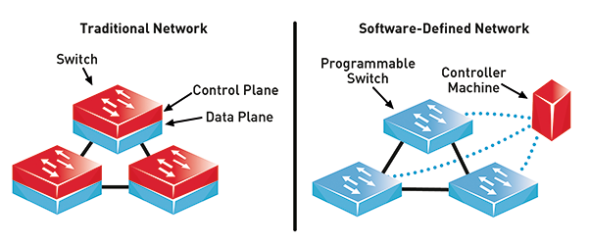
\includegraphics[width=6.5cm]{archivos/img/intro/sdn.png}
    \caption{Paradigma en redes \glsentryshort{sdn}}
    \label{sdnparadigma}
\end{figure}

Se considera como un punto de convergencia entre ambas tecnologías las redes 5G basadas fundamentalmente en \gls{sdn}, ya que prevén la incorporación de múltiples dispositivos \gls{iot}. Sin embargo, no todos los dispositivos \gls{iot} soportan una gestión basada en \gls{sdn} debido a las limitaciones que estos tienen en memoria, capacidad de procesamiento y  batería. Conforme el mundo de los dispositivos \gls{iot} avanza, las placas \gls{sbc} cada vez se hacen más potentes y de un tamaño más reducido, haciendo posible que éstas puedan ser incluidas como una pieza fundamental en proyectos \gls{iot} de alto rendimiento \cite{7501691}. \\

\par

Además, los sensores \gls{iot}, comúnmente conocidas como ``motas", continuamente se fabrican con más capacidad de procesamiento, memoria y batería con la finalidad de hacer frente a las nuevas redes de comunicaciones 5G \cite{capra2019edge}. Por todo ello,  se estima que la integración con las redes \gls{sdn} está cada vez más próxima. Generalmente, se están siguiendo estas vías de actuación:
\begin{itemize}
    \item \label{iot_integracionParcial}Realizar una integración parcial, haciendo uso de de dispositivos mediadores entre las motas y el core \gls{sdn}. Este dispositivo mediador, sería un dispositivo híbrido con interfaces inalámbricas y alámbricas para tener de acceso a la red \gls{sdn} \cite{7848825}. 
    
     \begin{figure}[h]
        \centering
        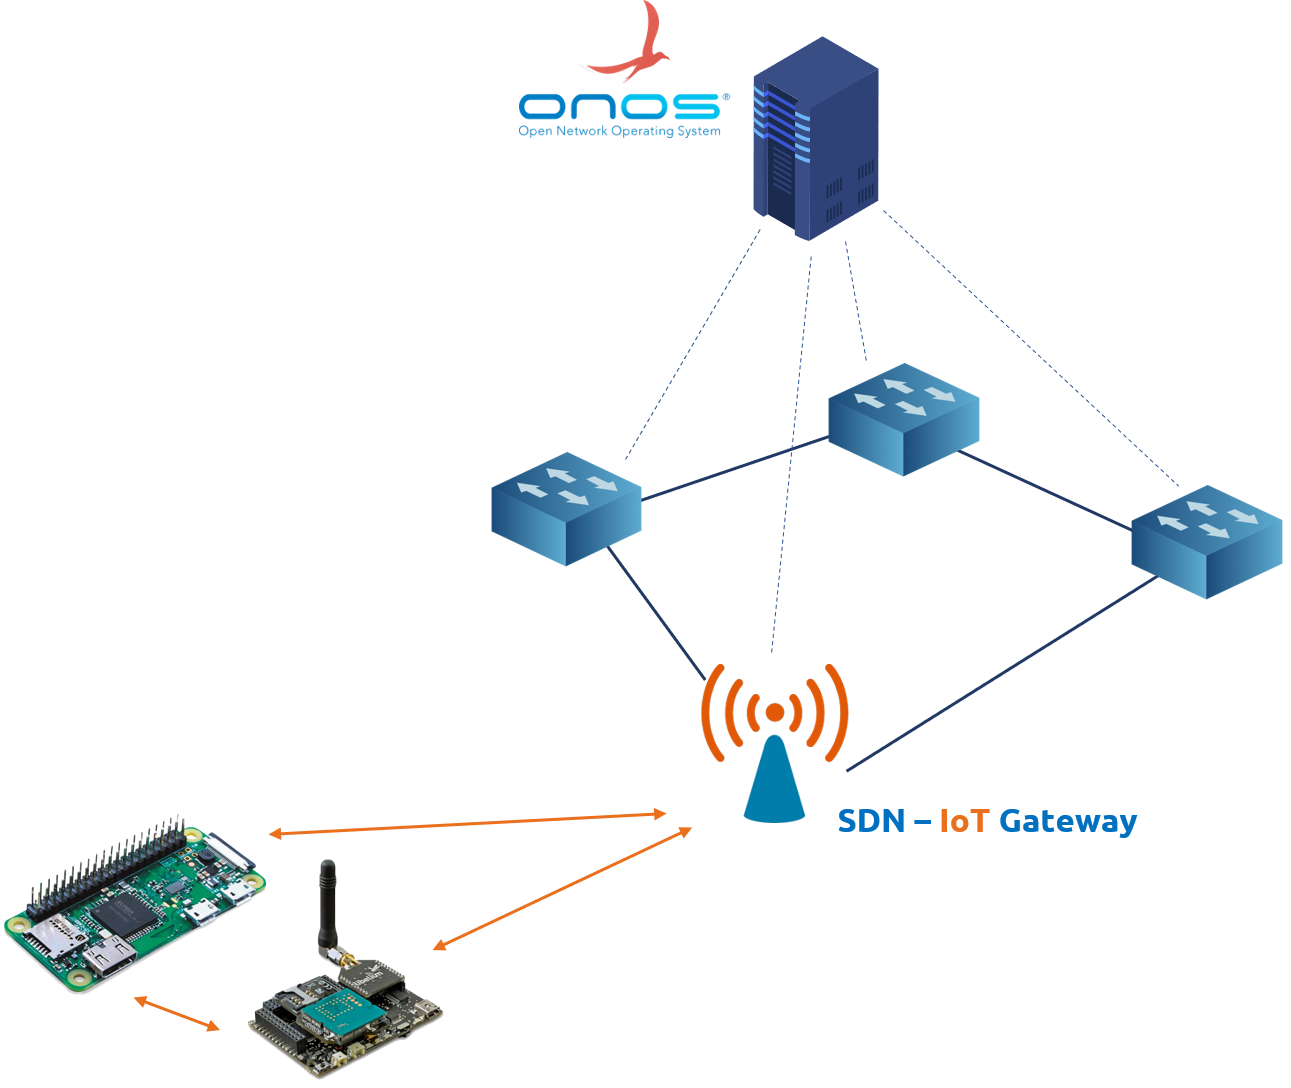
\includegraphics[width=10cm]{archivos/img/intro/sdn_iot.png}
        \caption{Integración parcial de dispositivos \glsentryshort{iot} en el core \glsentryshort{sdn}}
        \label{sdn_iot_parcial}
    \end{figure}
    Como se puede ver en la figura \ref{sdn_iot_parcial}, haciendo uso de un dispositivo mediador, este actuaría de pasarela o \textit{gateway} para las redes de sensores. De esta manera, se delega toda la carga de procesamiento y consumo de batería que supone integrar la interfaz de control \gls{sdn}. Además, se implementarían los distintos protocolos y estándares para comunicarse con los dispositivos \gls{iot}. Esta vía también ofrece otros aspectos positivos, entre los cuales se puede destacar, emplear el gateway como un traductor de protocolos \gls{iot} \cite{8470257}. Esto permitiría que distintos sensores que tuvieran implementados diferentes protocolos como, por ejemplo, \gls{ble}\footnote{Especificación del protocolo:  \url{https://www.bluetooth.com/specifications/}} y Zigbee\footnote{Protocolo de alto nivel basado en el estandar \gls{ieee} 802.15.4, especificación: \url{https://zigbeealliance.org/solution/zigbee/} }, pudieran interactuar entre sí a través del  gateway \gls{iot}.
    
    \item \label{iot_integracionTotal}Realizar una integración total, como se puede apreciar en la figura \ref{sdn_iot_total}, donde el propio dispositivo \gls{iot} es capaz de co-existir en la red \gls{sdn}. Esta última vía es la más ambiciosa debido a que se requiere de hardware lo suficientemente potente para soportar la lógica \gls{sdn}, y de una tecnología que establezca su plano de datos de forma más eficiente posible para optimizar al máximo los recursos limitados del dispositivo.
    
    \begin{figure}[ht]
        \centering
        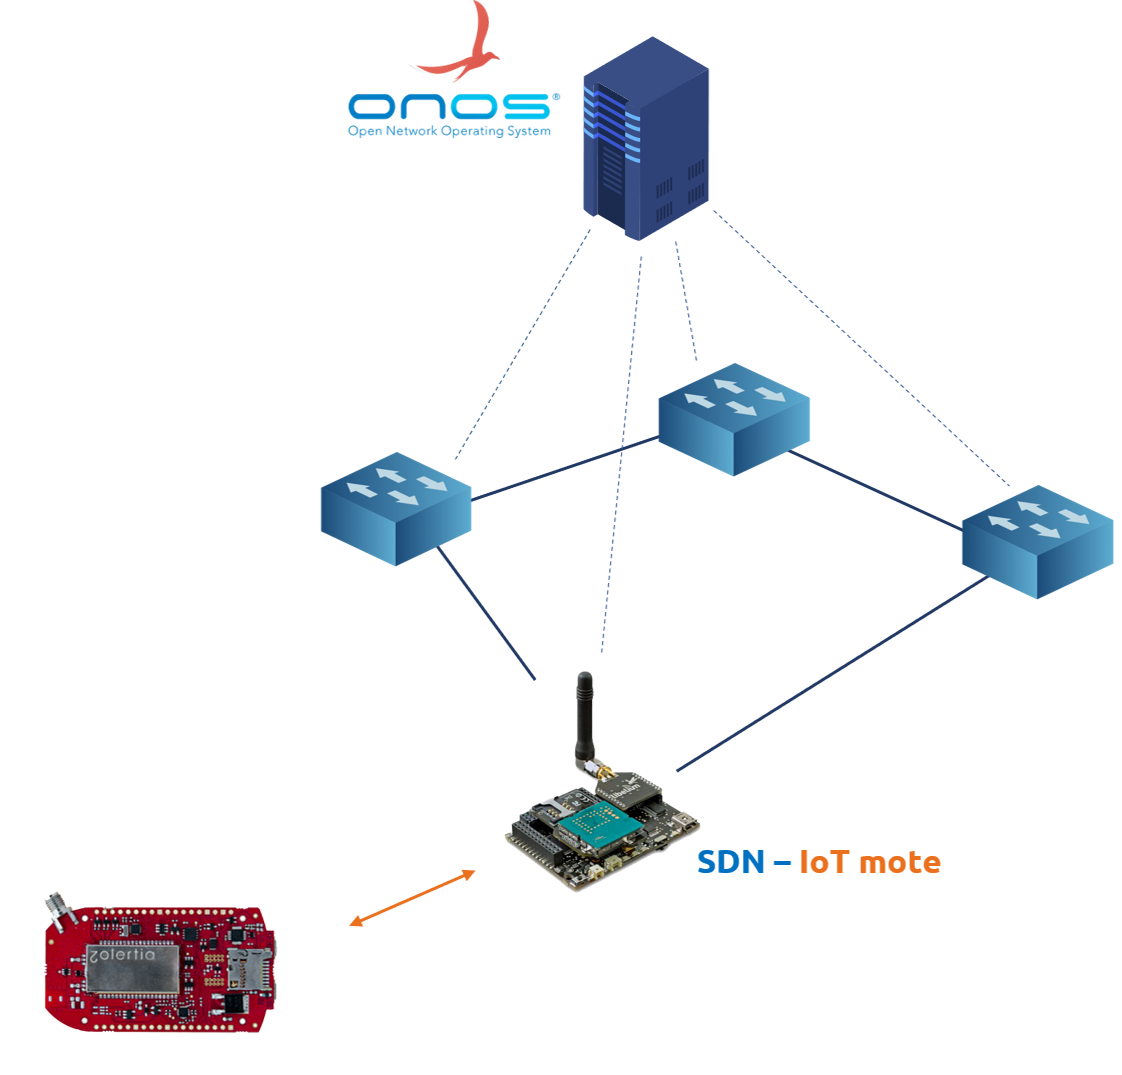
\includegraphics[width=10cm]{archivos/img/intro/sdn_iot_b.png}
        \caption{Integración total de dispositivos \glsentryshort{iot} en el core \glsentryshort{sdn}}
        \label{sdn_iot_total}
    \end{figure}
    
\end{itemize}



\section{Tecnologías para la definición del datapath}



En redes convencionales previas al concepto de \gls{sdn}, los nodos de la red tenían unificado un plano de control, \textit{Control plane}, donde se definía la lógica que dictaba como debía llevarse a cabo el \textit{forwarding} de los paquetes, y un plano de datos, \textit{Data plane}, el cual se puede implementar definiendo su datapath. Dicho datapath se compone de varios bloques de procesado para reenviar los paquetes. Con la llegada del paradigma de las redes \gls{sdn}, como se puede apreciar en la figura \ref{sdnparadigma}, los nodos clásicos de red verían como su plano de control sería delegado a una entidad llamada controlador. El controlador tendría una perspectiva global de toda la red en su conjunto pudiendo gestionarla de una manera más flexible y centralizada. \\
\par
En consecuencia, los nodos de la red estarían destinados a implementar un plano de datos, y una interfaz de control para ser configurados por el controlador mediante protocolos como, por ejemplo, OpenFlow\footnote{\url{https://www.opennetworking.org/software-defined-standards/specifications/}}. \\
\par
Por lo tanto, para ejecutar la integración de los dispositivos \gls{iot} en las redes \gls{sdn} se debe poder definir un datapath en dichos dispositivos y que estos posean una interfaz de control para ser configurados desde un hipotético controlador. Debido a esto, se requiere hacer uso de tecnologías que nos permitan definir el plano de datos de estos dispositivos. En este \gls{tfg}, se abordarán las siguientes tecnologías:

\begin{itemize}
    \item El lenguaje \textbf{P4}. Este lenguaje de alto nivel nos permite definir el procesado de los paquetes para un conjunto de arquitecturas. Dichas arquitecturas tienen su propia especificación. Con ello, se quiere conseguir que los programas P4 sean independientes del \textit{hardware} donde se ejecute \cite{2014p4}.
    
    \item \textbf{\gls{xdp}}. Es un \textit{framework} programable y de alto rendimiento para el procesado de paquetes en el Kernel de Linux. El procesado de los paquetes se lleva a cabo en el punto más bajo de la pila de red de Linux, consiguiendo así añadir nuevas funcionalidades sin necesidad de modificar el propio Kernel. Además, el hecho de definir el procesado de paquetes casi en la propia interfaz, reporta un gran rendimiento ya que no es necesario atravesar toda la pila de protocolos, con todo lo que eso conlleva (reservas de memoria, reservas de memoria para metadatos, encolado de los paquetes, desencapsulado de cabeceras, análisis y tratamiento de cabeceras, etc) \cite{xdp1}. 
\end{itemize}



\section{Objetivos}

El objetivo de este proyecto es realizar un estudio y análisis de las tecnologías P4 y \gls{xdp} para la integración de dispositivos \gls{iot} en entornos \gls{sdn}. Como ya hemos introducido, con la llegada del \gls{iot}, la dimensión de las redes va a crecer exponencialmente. Por consiguiente, la complejidad de la administración de dichas redes va a suponer un gran desafío.  Los dispositivos \gls{iot} se podrán beneficiar de la integración con las redes \gls{sdn}, ya que éstas les reportarán la \textbf{flexibilidad} y \textbf{programabilidad} requerida para una correcta gestión y administración de cada elemento de la red. Para alcanzar dicho objetivo, se han planteado los siguientes puntos:

\begin{itemize}
    \item \textbf{Documentación y estudio}: Búsqueda y recolección de información, artículos y guías para tener
los conocimientos básicos necesarios sobre el estado del arte actual y de las tecnologías para definir el plano de datos. De esta forma, se podrá plantear los diseños y desarrollos más optimizados, de cara a favorecer las limitaciones impuestas por los dispositivos \gls{iot}.

    \item \textbf{Planteamiento de casos de uso típicos y elección de escenarios}: Se hará un planteamiento de funcionalidades básicas, casos de uso, que una tecnología que define un datapath debe ser capaz de proveer. Además, se elegirán los escenarios y plataformas para desplegar dichos casos de uso.
    
    \item  \textbf{Desarrollo de los casos de uso}: Se abordará el desarrollo de dichos casos de uso con ambas tecnologías (P4, \gls{xdp}) en los escenarios planteados. Se tratará que los escenarios donde se desplieguen los desarrollos sean lo más homogéneos posibles, para que los puntos fuertes y débiles de cada tecnología puedan ser esclarecidos. 
    
    \item \textbf{Evaluación y comprobación de funcionamiento}: Se comprobará el correcto funcionamiento de todos los casos de uso desarrollados y por último, se evaluará que tecnología es más idónea para definir el datapath de los dispositivos \gls{iot} en su integración en entornos \gls{sdn}. 
\end{itemize}


\section{Estructura del \glsentryshort{tfg}}

En esta sección se indica la estructura básica de este \gls{tfg}, haciendo un breve resumen de los aspectos más importantes y significativos de cada capítulo. 


\begin{description}
\item\textbf{Capítulo 1: Introducción}. Se hará una breve introducción de la motivación que ha originado la realización de este \gls{tfg}, así como una breve explicación de los aspectos generales y de los objetivos que se quieren alcanzar con el trabajo presentado. 

\item\textbf{Capítulo 2: Estado del arte}. Se documentarán conceptos fundamentales en relación al proyecto, además de todas las diferentes herramientas que sean utilizadas. La motivación de este capítulo es la de establecer un marco teórico lo suficientemente consistente para abordar el análisis y el diseño de forma óptima, previo al desarrollo.

\item\textbf{Capítulo 3: Diseño y análisis de casos de uso}. Se debatirá y analizará que funcionalidades básicas deben tener las distintas tecnologías para definir el datapath. Para ello, se diseñarán distintos casos de uso para así demostrar la eficiencia de una tecnología sobre la otra en la integración de los dispositivos \gls{iot} en entornos \gls{sdn}.

\item\textbf{Capítulo 4: Desarrollo y evaluación de casos de uso}. Se describirá el desarrollo realizado, indicando las partes más importantes de cada caso de uso, ofreciendo al final de cada caso una evaluación de su funcionamiento. 

\item\textbf{Capítulo 5: Conclusiones y trabajo futuro}. Se terminará la memoria con las conclusiones del trabajo realizado, y se presentarán las vías de trabajo futuro que tiene este proyecto.

\item[]\textbf{Bibliografía y referencias}. Se añadirán todos los artículos, libros, materiales consultados y empleados en la elaboración de esta memoria. Se seguirá el estilo de citación del \gls{ieee}, siguiendo las recomendaciones oficiales de la normativa sobre \gls{tfg}s de la \gls{uah}. 

\item[]\textbf{Anexos}. Se incluirán todos los manuales de usuario e instalación que se consideren oportunos. De forma adicional, se añadirán las características técnicas del \textit{hardware} con el cual se ha desarrollado este \glsentryshort{tfg}. Por último, se hará un presupuesto que incluya el coste de mano de obra, material y gastos generales.

\end{description}

%%%%%%%%%%%%%%%%%%%%%%%%%%%%%%%%%%%%%%%%%%%%%%%%%%%%%%%%%%%%%%%%%%%%%%%%%%%%%%%%%%%%%%%%%%%%%%%%%%%%	
\chapter{Estado del arte}
\label{estadoArte}

En este capítulo se documentarán los conceptos fundamentales en relación al proyecto, además de todas las diferentes herramientas que sean utilizadas mayoritariamente. La motivación de este capítulo es la de establecer un marco teórico lo suficientemente consistente para abordar el análisis y el diseño de forma óptima, previo al desarrollo. Por último, se mencionará las contribuciones y la documentación generada con la intención de divulgar los contenidos de este proyecto a través de la herramienta \textit{GitHub}.


%%%%%%%%%%%%%%%%%%%%%%%%%%%%%%%%%%%%%%%%%%%%%%%%%%%%%%%%%%%%%%%%%%%%%%%%%%%%%%%%%%%%%%%%%%%%%%%%%%%%%
\section{Tecnología  \glsentryshort{sdn}}

El paradigma \gls{sdn} \cite{nadeau2013sdn} consiste en una arquitectura de red donde se lleva a cabo la separación del plano de control de la red para centralizarlo en un único ente llamado controlador. De esta forma se consigue que la administración de red sea una tarea más centralizada y flexible \cite{nadeau2013sdn}. La idea del \gls{sdn} empezó a germinar en la Universidad de Stanford por el año 2003, donde el profesor asociado en su momento, Nick McKeown, planteaba las limitaciones de las redes convencionales y veía la necesidad de replantear como los \textit{backbones} debían operar \cite{sdnBegins}. Dicha idea se acuñó como \gls{sdn} en el año 2011, cuando a la par se lanzó la organización \gls{onf} \cite{onf} como un portador de los estándares relacionados con el \gls{sdn} y su difusión.

\subsection{Arquitectura}

La arquitectura \gls{sdn} destaca por ser dinámica, rentable y adaptable haciéndola ideal para las demandas presentadas hoy en día por las redes de comunicaciones. Como ya se ha comentado, la arquitectura se basa en separar el plano de control del plano de datos, y llevar ese plano de control a una entidad llamada controlador. Desde dicha entidad se ofrecerán las interfaces necesarias para que aplicaciones de servicios de red puedan hacer uso de ellas. De esta forma, el control de la red se vuelve directamente programable, consiguiendo que la gestión se vuelva más ágil y dinámica.\\
\par

Como se puede ver en la figura \ref{fig:sdnBasicArch}, la arquitectura \gls{sdn} se divide en tres capas, la primera, el plano de datos que contendrá todos los elementos de red que habiliten el forwarding. La segunda, el plano de control, compuesto de los distintos controladores de la red \gls{sdn}, y por último, la capa de aplicación, en la cual se encontrarán todas las aplicaciones que se comuniquen con el controlador \gls{sdn}. \\
\par
Dichas capas se comunicarán entre ellas a través de interfaces abiertas. Por ejemplo, la interfaz \textit{Southbound} permite programar el estado de reenvío de los elementos de red del plano de datos. En cambio, la interfaz \textit{Northbound} comunica las aplicaciones con los controladores \gls{sdn}, habilitando la obtención de datos o el ajuste de parámetros a través de una API-Rest. También se pueden encontrar otro tipo de interfaces, \textit{Westbound} y \textit{Eastbound}, que se han consolidado los últimos años para la interconexión de controladores con la finalidad de establecer una misma política entre distintos dominios \gls{sdn}.

% Foto 
\begin{figure}[ht]
    \centering
    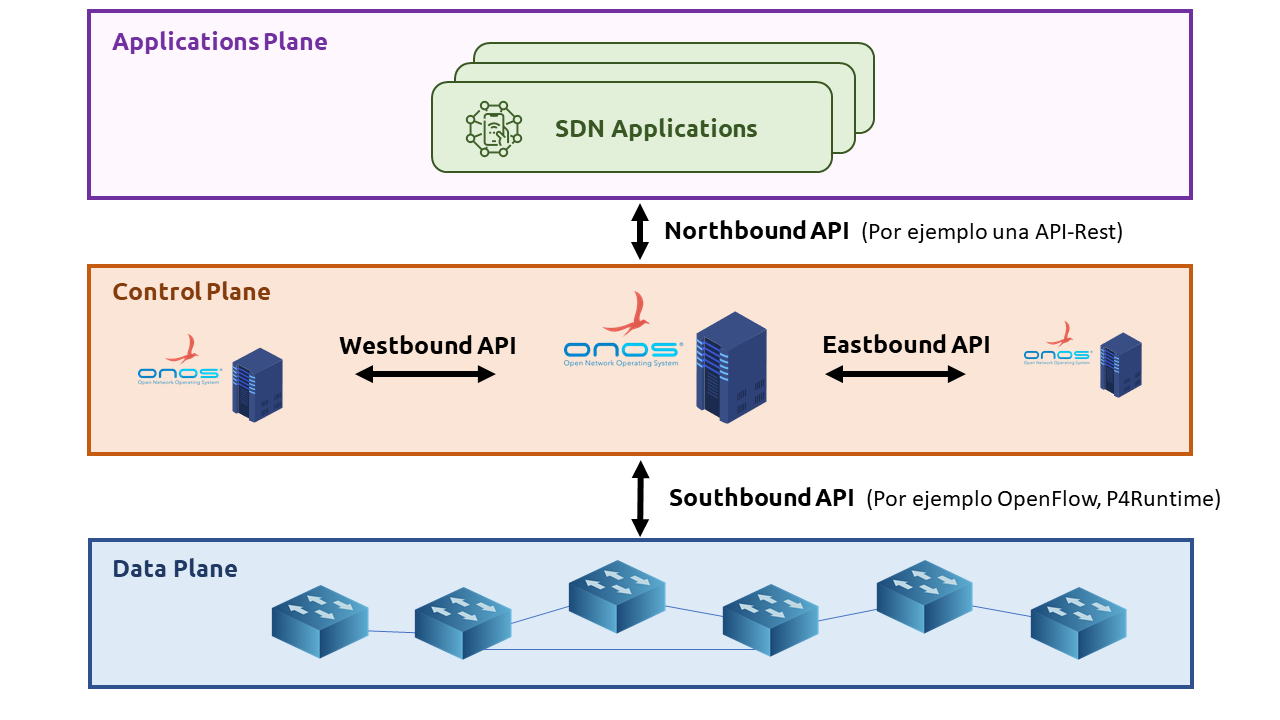
\includegraphics[width=14.5cm]{archivos/img/teoria/sdn_arch.png}
    \caption{Arquitectura básica \glsentryshort{sdn}}
    \label{fig:sdnBasicArch}
\end{figure}

\subsection{OpenFlow}

Existen varios protocolos para el control de los elementos de red desde el controlador, pero el más utilizado es Openflow. OpenFlow es un protocolo de la interfaz \textit{Southbound} que comunica los controladores \gls{sdn} con los elementos de red para configurar el estado de reenvío de estos últimos. La especificación de este protocolo se encuentra recogida por la \gls{onf}\footnote{\url{https://www.opennetworking.org/software-defined-standards/specifications/}}, contando con numerosas versiones siendo la última la versión \texttt{1.5.1} del 2015. \\
\par

El elemento clave de OpenFlow es el flujo (\textit{flow}), los cuales se conforman de paquetes que ha sido clasificados en función de reglas. Dichas reglas se encuentran en las tablas de flujo (\textit{flow table}) y  suelen estar relacionadas con los puertos de entrada o valores de cabecera típicos. Cuando estos criterios coinciden con los del paquete entrante se produce un \textbf{\textit{match}}.\\
\par
En el momento en que se produce un \textit{match}, el paquete en cuestión se verá sujeto a una serie de instrucciones asociadas a la regla con la que a hecho \textit{matching}. Estas instrucciones pueden ir desde, hacer una medición del paquete, aplicar una acción ó ir a otra tabla de flujo. De esta forma, con unas tablas de flujo completadas con unas reglas suministradas por el controlador \gls{sdn}, se conforma el estado de reenvío del switch en cuestión \cite{nadeau2013sdn}. 



%%%%%%%%%%%%%%%%%%%%%%%%%%%%%%%%%%%%%%%%%%%%%%%%%%%%%%%%%%%%%%%%%%%%%%%%%%%%%%%%%%%%%%%%%%%%%%%%%%%%%


\section{Tecnología \glsentryshort{iot}}
\label{iot}

La premisa básica de la tecnología \gls{iot} \cite{iotreview} conectar cualquier dispositivo que tenga cierta capacidad de cómputo. Esto significa que los objetos que actualmente no están conectados a Internet, estarán conectados de manera que puedan comunicarse e interactuar con personas y otros objetos. \\
\par

La tecnología \gls{iot} es una transición tecnológica en la que los dispositivos al ser dotados de inteligencia por estar conectados a Internet podrán proveer de entornos inteligentes a los humanos.  Cuando los objetos puedan ser controlados a distancia a través de una red, se habilitará una integración más estrecha entre el mundo físico y las máquinas, permitiendo mejoras en las áreas de medicina, automatización y logística \cite{7073822}.\\
\par

El ecosistema \gls{iot} es amplio, e incluso se puede parecer un poco caótico debido a la gran cantidad de componentes y protocolos que abarca. Es recomendable en vez de ver el \gls{iot} como un termino único, verlo como un paraguas de varios conceptos, protocolos y tecnologías, enfocados a un mismo propósito de interconectar ``Cosas" a Internet. Si bien la amplia mayoría de elementos \gls{iot} están diseñados para aportar numerosos beneficios en las áreas de productividad y automatización, al mismo tiempo introducen nuevos desafíos, como por ejemplo la gestión de la gran cantidad de dispositivos que van a aparecer en las redes, y la cantidad de datos y mensajes que todos estos generaran \cite{iotreview}.

\subsection{Arquitectura}

Aunque en el ecosistema hay diferentes \textit{stacks} de protocolos, todos ellos se pueden resumir en la siguiente arquitectura básica \cite{iotreview}.

\begin{itemize}
    \item \textit{Perception Layer}, en esta capa se da un significado físico a cada objeto. Consiste en sensores de diferentes tipos como etiquetas RFID, sensores IR u otras redes de sensores que podrían detectar la temperatura, la humedad, la velocidad y la ubicación, etc. Esta capa recolecta información útil a partir de los sensores vinculados a los objetos,  convierte dicha información en señales digitales que más tarde se delegarán a la Capa de Red para su posterior transmisión.
    
    \item \textit{Network Layer}, el propósito de esta capa es la de recibir la información en
    forma de señales digitales desde la capa de Percepción y transmitirla a los sistemas de procesamiento en la capa de \textit{Middleware}. Esto se llevará a cabo a través de las distintas tecnologías de acceso como WiFi, BLE, WiMaX, ieee802154 y con protocolos como IPv4, IPv6, MQTT.
    
    \item \textit{Middlware Layer}, en esta capa se procesa la información recibida de todos los sensores. En esta capa se puede incluir las tecnologías como Cloud computing, o sistemas gestores,  que aseguran un acceso directo a bases de datos donde se puede almacenar toda la información recolectada. Teniendo una gran cantidad de información centralizada, generalmente se aplican sistemas de inteligencia artificial para procesar la información, y tomar decisiones predictivas totalmente automatizadas. Estos sistemas suelen ser utilizados para analizar el tiempo, contaminación o tráfico en las ciudades. 
    
    \item \textit{Application Layer}, la finalidad de  esta  capa es la de realizar las aplicaciones \gls{iot} para el usuario final. Estas aplicaciones se valdrán de los datos procesados para ofrecer funcionalidades al usuario final, por ejemplo, una aplicación del tiempo.
    
    \item \textit{Business Layer}, esta capa aunque es un poco abstracta, se suele añadir para representar la gestión de múltiples las aplicaciones y servicios \gls{iot}. 
\end{itemize}

% Foto 
\begin{figure}[ht]
    \centering
    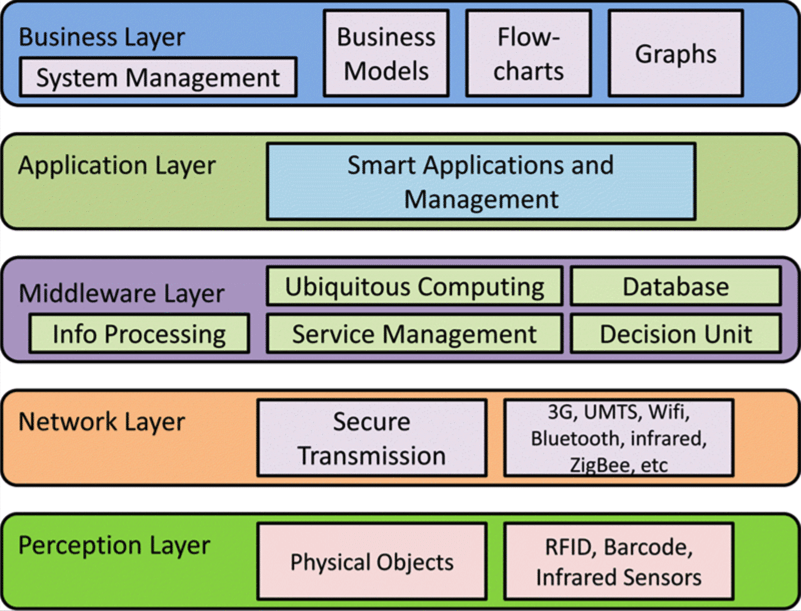
\includegraphics[width=6.5cm]{archivos/img/teoria/arch_edited.png}
    \caption{Arquitectura básica \glsentryshort{iot}}
    \label{fig:iotBasicArch}
\end{figure}

\subsection{Topologías}

Entre las tecnologías de acceso disponibles para conectar los dispositivos de \gls{iot}, dominan tres esquemas topológicos principales, estrella, malla y p2p. Para las tecnologías de acceso de largo y corto alcance, predomina la topología de estrella, como se puede encontrar en las redes datos móviles, LoRa y BLE. Las topologías en estrella utilizan una única estación base central para permitir las comunicaciones con los nodos finales. En cuanto a las tecnologías de mediano alcance, se pueden encontrar topologías en estrella, de p2p o en malla, como se ve en la figura \ref{fig:iotTopo}. Generalmente se suele hacer uso de un tipo de topología sobre otra en función de las limitaciones de los nodos que la conforman \cite{iotbook}.\\
\par

% Foto 
\begin{figure}[ht]
    \centering
    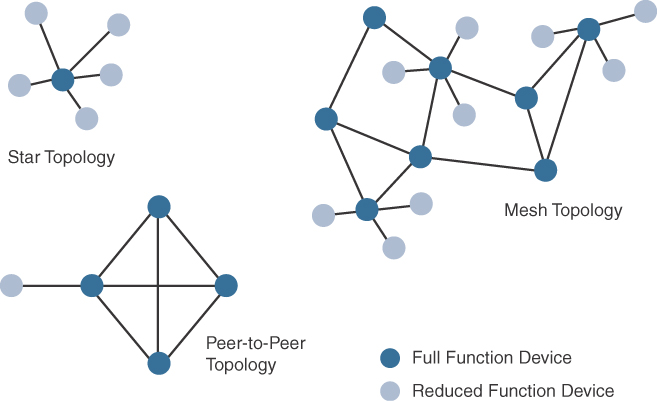
\includegraphics[width=7.5cm]{archivos/img/teoria/iot_topo.jpg}
    \caption{Tipos de topología con dispositivos \glsentryshort{iot} \cite{iotbook}}
    \label{fig:iotTopo}
\end{figure}


\subsection{Redes LLN}

Las redes de baja capacidad, conocidas como, \gls{lln}\footnote{\url{https://tools.ietf.org/html/rfc7228}}, se caracterizan por estar compuestas de dispositivos (sensores, motas) con limitaciones de memoria, batería y procesamiento. Dichos nodos, se interconectarán haciendo uso de distintos de tipos de enlace, como por ejemplo \texttt{ieee802154} ó LowPower-WiFi \cite{llnrfc}. Este tipo de redes pueden estar presentes en distintos campos de aplicación, entre las que se incluyen asistencia sanitaria, monitorización industrial, redes de sensores, etc.   \\

\par
Otra condición de las redes \gls{lln}, son las pérdidas en capa física debidas a las interferencias y variabilidad de los ``complicados" entornos radio donde estarán desplegadas dichas redes. Por ello, y teniendo en cuenta que los nodos que formarán parte de las redes \gls{lln} serán de baja capacidad, es necesario que los protocolos utilizados en esta red sean capaces de optimizar al máximo los recursos de los dispositivos \cite{iotbook}. 

\subsubsection{IEEE 802.15.4}

El estándar \texttt{ieee802154}\footnote{\url{https://tools.ietf.org/id/draft-ietf-lwig-terminology-05.html}} define la tecnología acceso a un entorno inalámbrico (\textit{phy} y \textit{mac}) para dispositivos de baja capacidad (limitados en batería y capacidad de transmisión). Este estándar se caracteriza por la optimización de los recursos del nodo en cuestión, consiguiendo una duración prolongada de la batería, además, esta tecnología de acceso permite un fácil uso utilizando un \textit{stack} de protocolos compacto, al tiempo que sigue siendo simple y flexible. Por todas estas características, el estándar \texttt{ieee802154} es usado en la mayoría de \textit{stack} de protocolos enfocados al \gls{iot}. Uno de los más utilizados es el \textit{stack} 6LoWPAN, definido por el \gls{ietf}, consiste en una capa de adaptación de IPv6 sobre las capas del estándar \texttt{ieee802154} (Ver figura \ref{fig:6lowapan}) \cite{6lowpan}.\\
\par

\vspace{0.5cm}

% Foto 
\begin{figure}[ht]
    \centering
    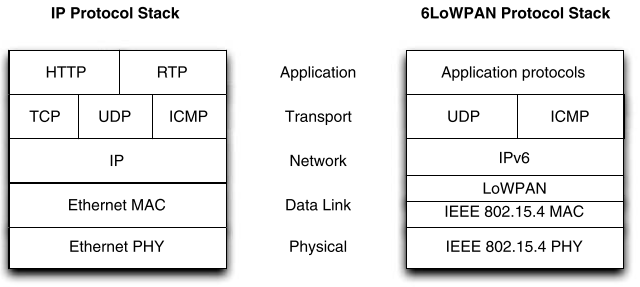
\includegraphics[width=12cm]{archivos/img/teoria/6LoWPAN-Protocol-Stack.png}
    \caption{Pila de protocolos 6LoWPAN \cite{6lowpan}}
    \label{fig:6lowapan}
\end{figure}



%%%%%%%%%%%%%%%%%%%%%%%%%%%%%%%%%%%%%%%%%%%%%%%%%%%%%%%%%%%%%%%%%%%%%%%%%%%%%%%%%%%%%%%%%%%%%%%%%%%%%

\newpage
\section{Tecnología P4}
\label{TecnologiaP4}

La tecnología P4\footnote{\textit{\textbf{P}rogramming \textbf{P}rotocol-independent \textbf{P}acket \textbf{P}rocessors}} se diseñó principalmente como un lenguaje de alto nivel para programar procesadores de paquetes. Su impulso vino de la mano de un consorcio de empresas privadas relacionadas con el mundo de las telecomunicaciones y fabricantes de hardware, conocido como P4 Language Consortium. Más tarde, conforme la tecnología fue ganando fuerza, el proyecto P4 pasó a ser parte de la \gls{onf} ganando así más difusión en la comunidad.\\
\par
Dicha tecnología nació con el propósito de cubrir las limitaciones del protocolo OpenFlow. El protocolo OpenFlow a través de distintas versiones había aumentado la cantidad de campos de cabeceras, admitiendo así más protocolos, pasando de 12 campos a 41 en cuatro años. Este hecho supuso un aumento en la complejidad de la especificación del protocolo, y aún seguían limitados en dar flexibilidad para añadir nuevas cabeceras \cite{2014p4}.\\
\par
Debido a lo cual, se presentaba P4 como una solución hacia donde debía evolucionar OpenFlow. Para ello, se basaron en tres pilares fundamentales, el primero de ellos era conseguir que los dispositivos de red fuera reconfigurables en vuelo, el segundo consistía en que los switches fueran agnósticos a cualquier protocolo de red, y por último, se quería que el lenguaje P4 fuera completamente independiente del hardware sobre el cual se fuera a implantar. 

% Foto elisa 
\begin{figure}[ht]
    \centering
    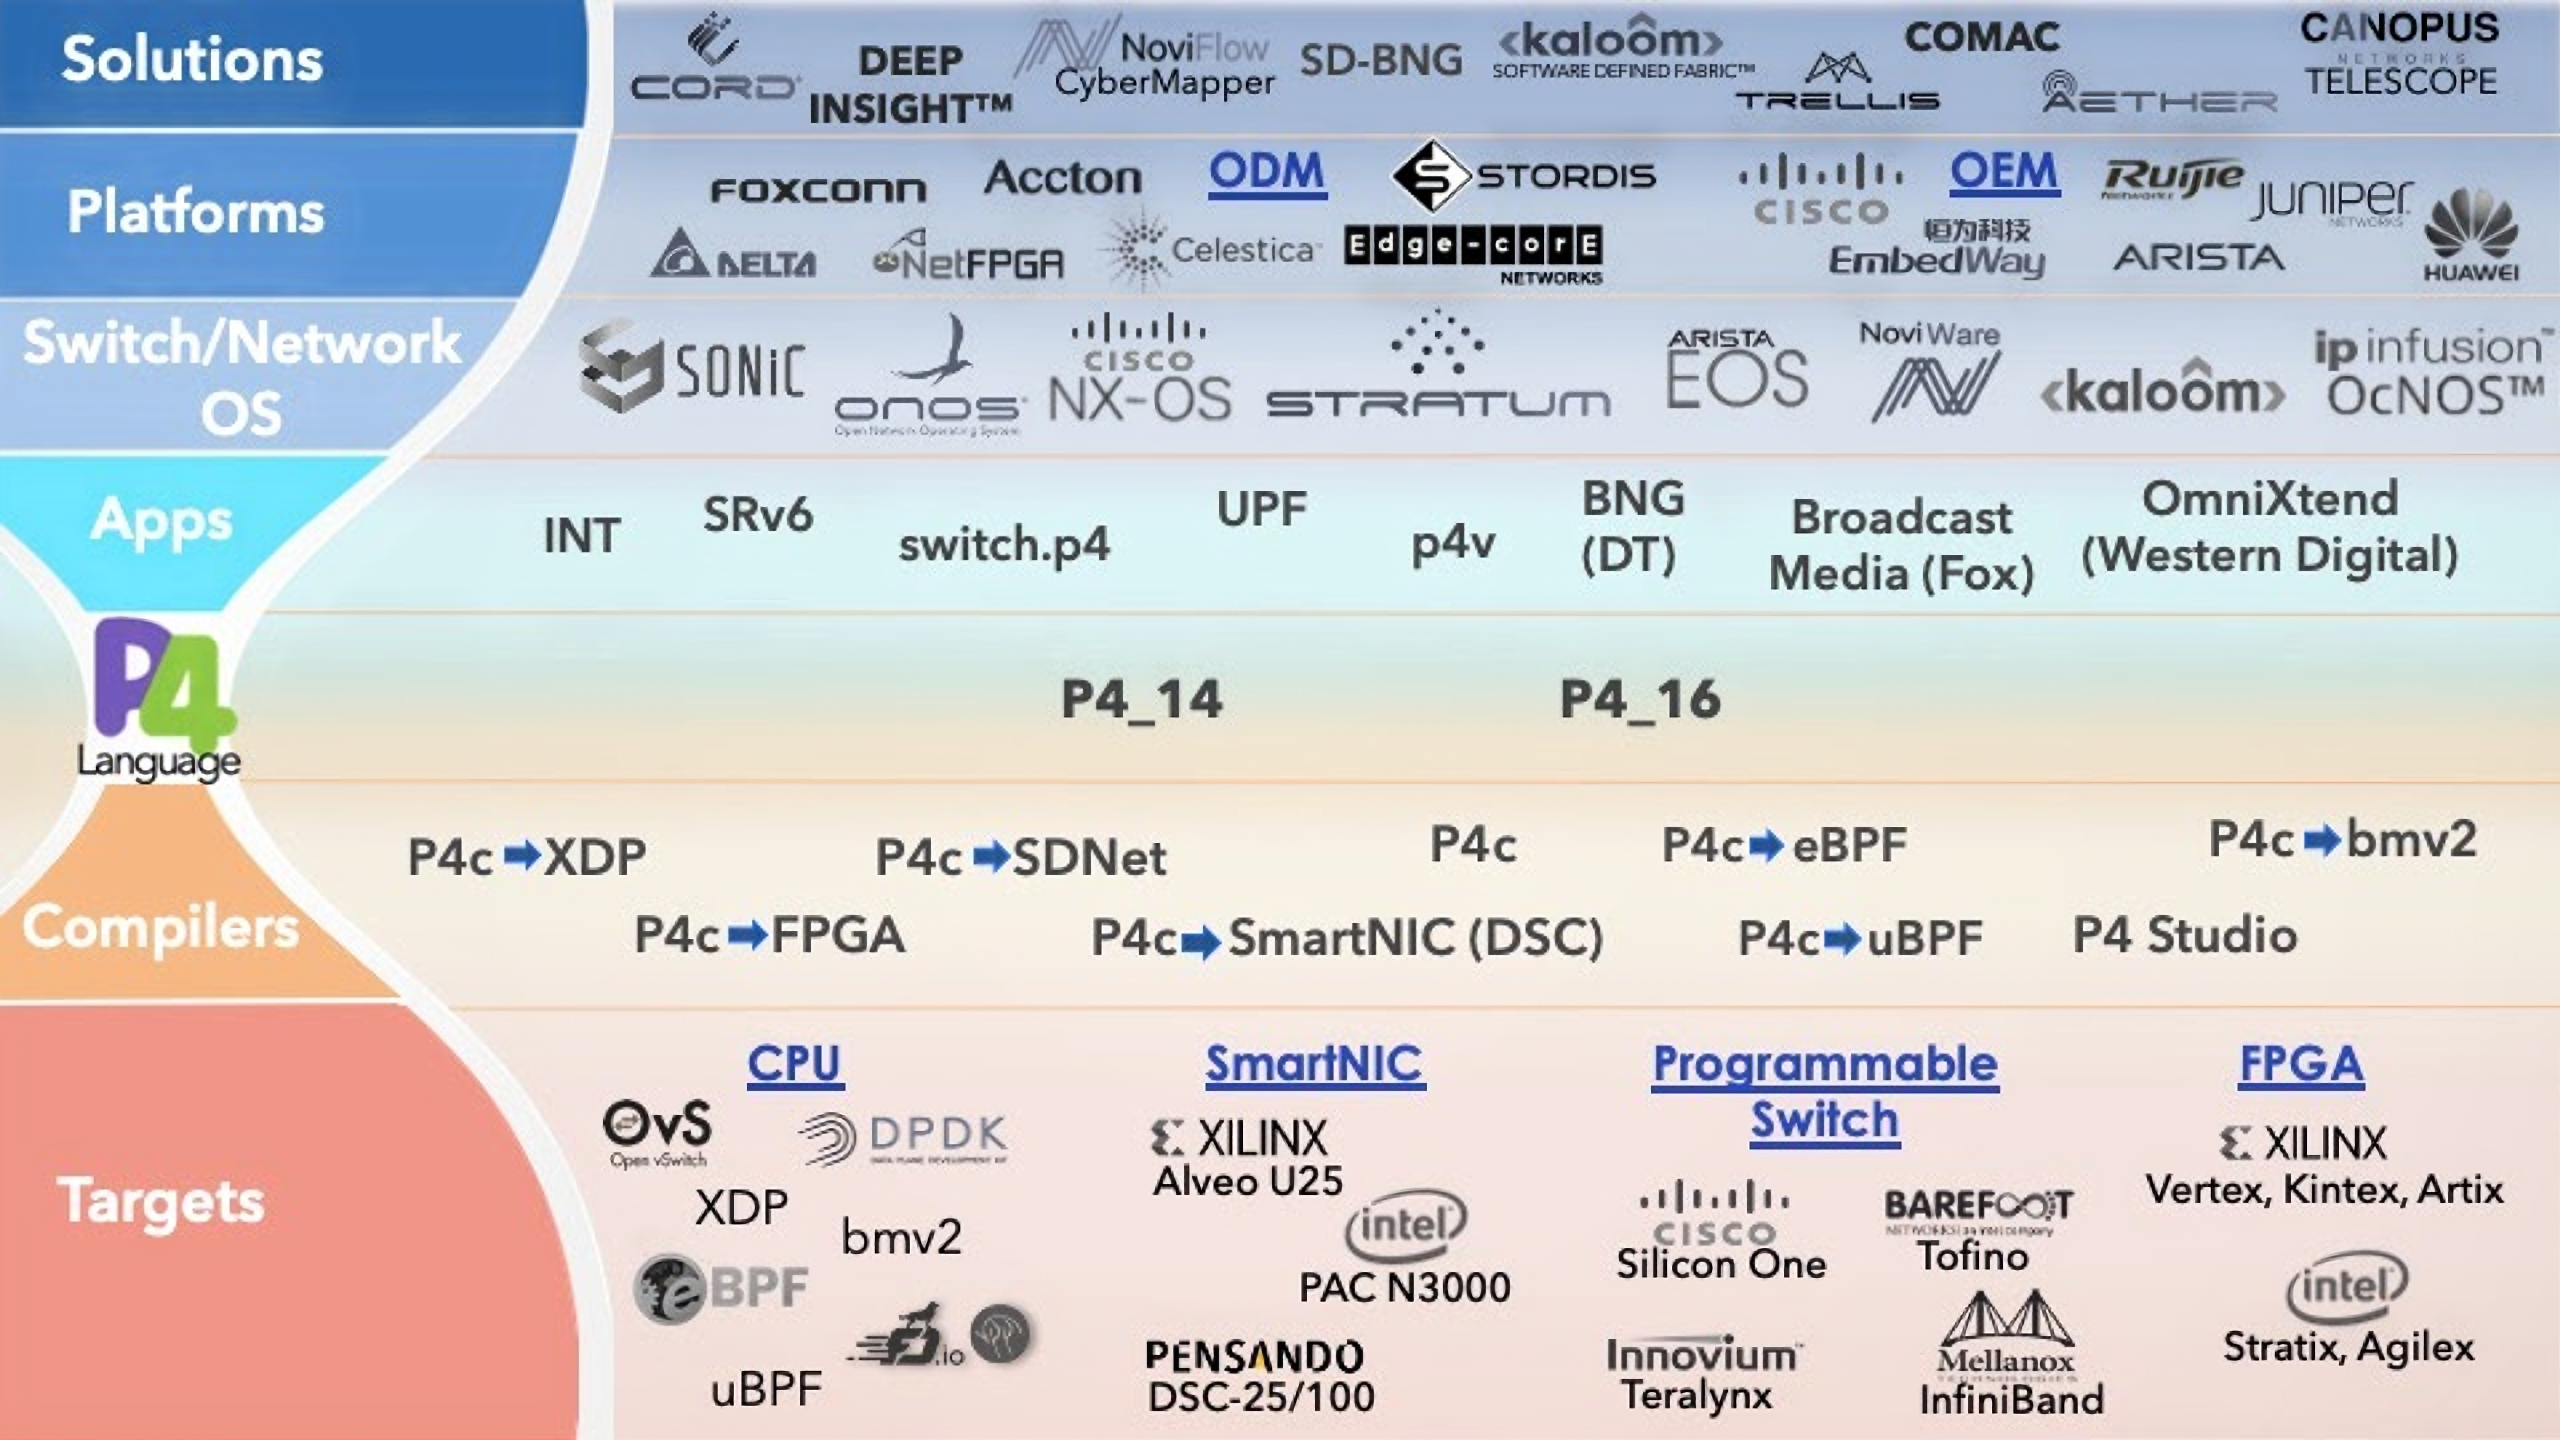
\includegraphics[width=14.5cm]{archivos/img/teoria/p4resumen_edited2.png}
    \caption{Ecosistema P4}
    \label{fig:p4eco}
\end{figure}

A día de hoy la tecnología P4 ya está ampliamente implantada. Como se puede apreciar en la figura \ref{fig:p4eco}, se ha generado todo un ecosistema entorno a esta tecnología, contando con numerosos compiladores de \textit{backend} enfocados para los distintos \textit{targets}, con aplicaciones y soluciones ya puestas en funcionamiento. Por lo que todo apunta a que este ecosistema tiende a ir a más, si bien es verdad que aún tiene ciertas dificultades con ciertos tipos de hardware, pero su futuro es bastante prometedor. 


%%%%%%%%%%%%%%%%%%%%%%%%%%%%%%%%%%%%%%%%%%%%%%%%%%%%%%%%%%%%%%%%%%%%%%%%%%%%%%%%%%%
\subsection{Objetivos}

Por tanto, la llegada de la tecnología P4 supuso una cambio de paradigma a la hora de diseñar nuevos protocolos. Esto es así ya que permitía decir a los \textit{switches} como debían operan en vez de estar limitados por las condiciones de diseño del propio \textit{switch} (Ver figura \ref{fig:p4Paradigma}). Este paradigma se alcanzaría encontrando un termino medio entre la expresividad del lenguaje P4 y la compatibilidad de éste entre la gran mayoría de hardware y soft-switches. Por ello, se plantearon tres hitos a conseguir \cite{2014p4}.

\begin{itemize}
    \item \textbf{Reconfigurabilidad}. En un entorno \gls{sdn}, el controlador debería ser capaz de redefinir el \textit{datapath} de los \textit{switches}.
    \item \textbf{Agnóstico a protocolos}. Los switches no deben tener ningún conocimiento sobre los protocolos de red, es deber del controlador especificar como debe analizar y procesar los paquetes que le lleguen para extraer las cabeceras, y una serie de tablas del tipo \textit{match-action} para procesar esas cabeceras. 
    \item \textbf{Independencia de la arquitectura}. Al igual que los programadores de aplicaciones no tienen que especificar sobre que arquitectura están compilando su aplicación, se quería que los programadores de P4 no se preocuparan sobre en que arquitectura se iba a correr dicho programa P4. Será deber de los compiladores tomar el programa P4 totalmente independiente de arquitectura y convertirlo en un programa que dependa de la arquitectura en cuestión.
\end{itemize}

% Foto 
\begin{figure}[ht]
    \centering
    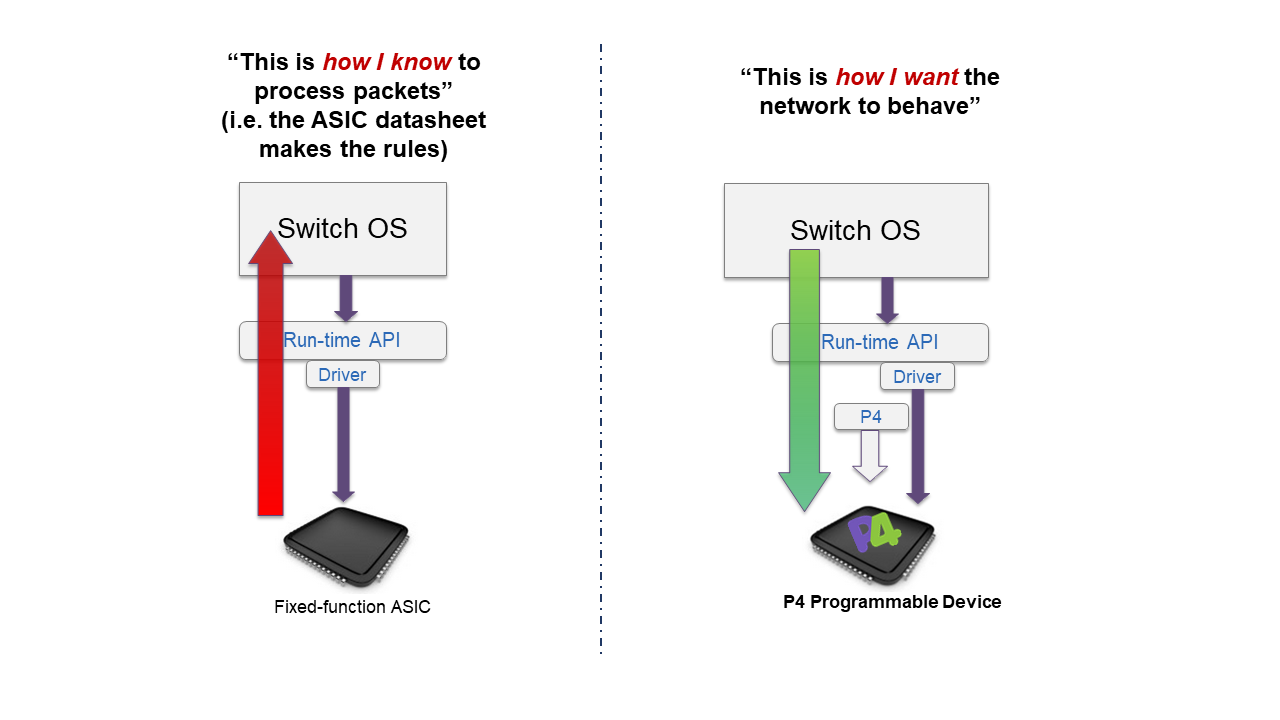
\includegraphics[width=13.5cm]{archivos/img/teoria/p4Paradigm.png}
    \caption{Cambio de paradigma con la tecnología P4 \cite{p42}}
    \label{fig:p4Paradigma}
\end{figure}


%%%%%%%%%%%%%%%%%%%%%%%%%%%%%%%%%%%%%%%%%%%%%%%%%%%%%%%%%%%%%%%%%%%%%%%%%%%%%%%%%%%
\subsection{Arquitectura y targets}

A partir de la especificación P4\textsubscript{16} se definen dos nuevos conceptos para conseguir alcanzar la independencia de los programas P4 de las distintas arquitecturas de cada fabricante. 

\begin{itemize}
    \item El concepto de \textit{Target}, se puede ver como una implementación del hardware/software especifica donde se va a correr un programa P4.
    \item El concepto de \textit{Architecture}, se puede definir como la interfaz presentada por el fabricante para programar un \textit{target} a través de componentes P4. 
\end{itemize}

% Foto 
\begin{figure}[ht]
    \centering
    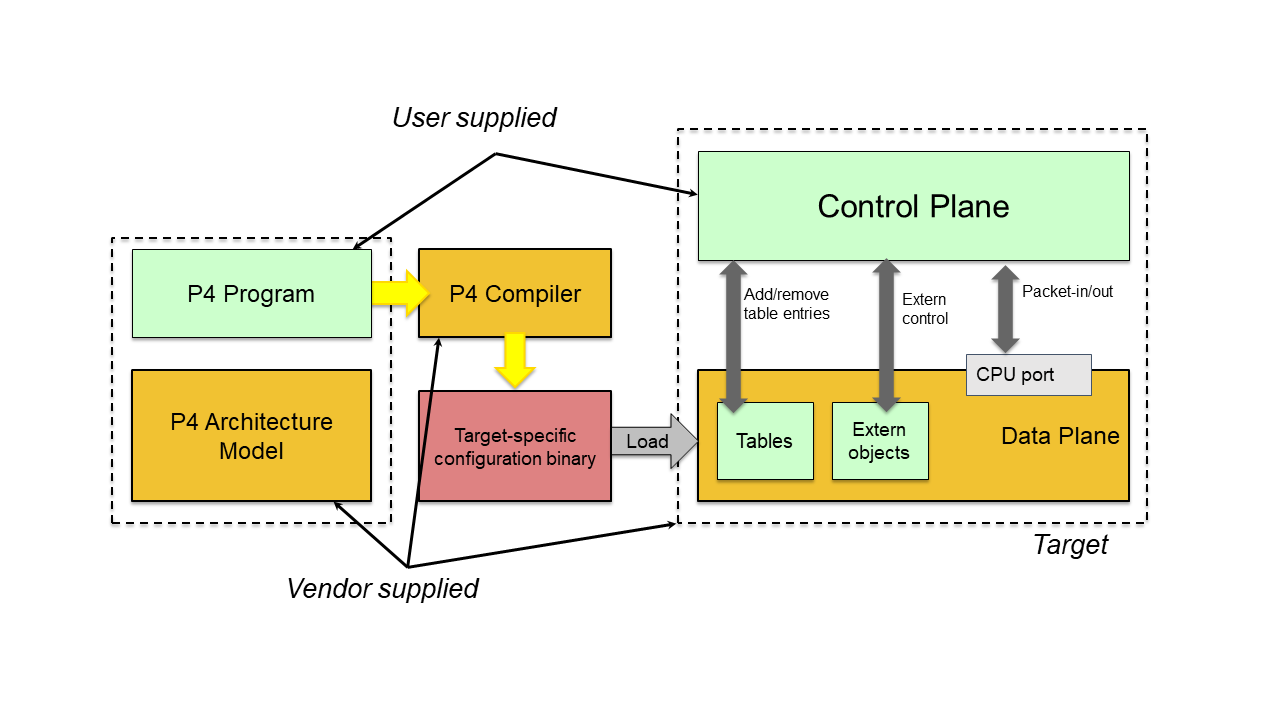
\includegraphics[width=14.5cm]{archivos/img/teoria/p4arch.png}
    \caption{Arquitectura de la tecnología P4 \cite{p42}}
    \label{fig:p4arch}
\end{figure}

Como se puede ver en la figura \ref{fig:p4arch}, el fabricante es el encargado de proveer la arquitectura, compilador y el \textit{target}. Y el usuario solo se tendrá que preocupar de escribir un programa P4 y definir la interfaz de control. De esta forma, se quiere conseguir que el usuario solo se preocupe en seguir la interfaz/arquitectura dada por el fabricante para programar un \textit{target} en especifico.\\
\par
Un programa P4 desarrollado para una arquitectura será exportable entre distintos \textit{targets} que implementen la misma arquitectura. Por lo que, si las arquitecturas como por ejemplo \texttt{v1model}, \texttt{PSA} se asientan entre los distintos fabricantes de hardware se conseguirá la independencia del hardware, para depender solo del software.  

%%%%%%%%%%%%%%%%%%%%%%%%%%%%%%%%%%%%%%%%%%%%%%%%%%%%%%%%%%%%%%%%%%%%%%%%%%%%%%%%%%%
% \subsection{Elementos del lenguaje P4}

% \begin{itemize}
%     % cabs
%     \item \textbf{Cabeceras},
    
%     % parsers
%     \item \textbf{Parsers},
    
%     % tablas
%     \item \textbf{Tablas},
    
%     % actions 
%     \item \textbf{Acciones}, 
% \end{itemize}











%%%%%%%%%%%%%%%%%%%%%%%%%%%%%%%%%%%%%%%%%%%%%%%%%%%%%%%%%%%%%%%%%%%%%%%%%%%%%%%%%%%%%%%%%%%%%%%%%%%%%

\newpage
\section{Tecnología \glsentryshort{xdp}}
\label{TecnologiaXDP}

La tecnología \gls{xdp}, es una tecnología para procesar paquetes, programable, de alto rendimiento e integrada en el \textit{datapath} del Kernel de Linux. Esta tecnología se basa en ejecutar \textit{bytecodes} \gls{bpf} cuando la interfaz sobre la cual está anclado un programa \gls{xdp} recibe un paquete. Esto habilita que ciertas decisiones para según que paquetes, se realicen lo antes posible casi en la propia interfaz, quitándose de encima todas las capas del \textit{stack} que harían operaciones redundantes.\\
\par

Pero el hecho de que se ejecute casi en la propia interfaz no es la única razón del alto rendimiento de los programas \gls{xdp}. Otras decisiones que han sido vitales para hacer de esta tecnología una pieza clave para las nueva generación de herramientas\footnote{\url{https://git.kernel.org/pub/scm/linux/kernel/git/netdev/net-next.git}} en Linux.

\begin{itemize}
    \item No se reserva memoria mientras se hace el procesamiento de paquetes con \gls{xdp}.
    \item No se emplea las estructuras \texttt{sk\_buff} para gestionar la información de metadatos de los paquetes, en cambio se hace uso de una estructura \texttt{xdp\_buff} la cual no contiene tanta información en exceso. 
    \item No se permiten bucles, ni un número excesivo de iteraciones en los programas anclados a la \gls{nic}.
    
\end{itemize}


\par

El funcionamiento de un programa \gls{xdp} se basa generalmente en analizar un paquete, editarlo en caso de que sea necesario y por último, devolver un código de retorno que indique que se debe hacer con dicho paquete. Los códigos de retorno \gls{xdp}, se utilizan para determinar qué acción se va a tomar con el paquete, estas acciones pueden ser muy variadas, desde hacer que el paquete sea descartado, hasta delegarlo al \textit{stack} de red para que se encargue este del procesado, o reenviar el paquete para que sea transmitido de nuevo. \\
\par

Antes se mencionaba que los programas \gls{xdp}, consistían en ejecutar \textit{bytecodes} \gls{bpf} cuando llega un paquete a la interfaz donde está cargado el programa, pero, ¿Qué relación existe entre \gls{xdp} y \gls{bpf}? Resulta que todos los programas \gls{xdp} que se escriben en un C restringido, se compilarán haciendo uso del compilador de \textbf{clang}\footnote{Compilador de tipo frontend de referencia de la familia del lenguaje C.} como \textit{frontend} y del compilador \textbf{LLVM}\footnote{Infraestructura para implementar compiladores de forma agnóstica al lenguaje a compilar, generalmente usado como compilador de Backend.} como \textit{backend}, para conseguir un \textit{bytecode} \gls{bpf}.\\
\par

La motivación de esta ``traducción" radica en  que los programas XDP son cargados en el Kernel a través de la llamada al sistema \gls{bpf}, indicando que se trata de un tipo de programa \gls{xdp} con la macro, \texttt{BPF\_PROG\_TYPE\_XDP}. De esta forma, se permite reutilizar los mecanismos de carga de \textit{bytecodes} en el Kernel utilizados con \gls{bpf}, pero en este caso con \gls{xdp} estarán únicamente enfocados en la carga de dichos \textit{bytecodes} en la \gls{nic}. Por lo que, \gls{xdp} se podría ver como un \textit{framework} \gls{bpf} diseñado para trabajar en la interfaz, con limitaciones y pautas de desarrollo muy marcadas para conseguir que la tecnología sea de alto rendimiento \cite{xdp1}.\\
\newpage

\subsection{Modos de operación}

\begin{table}[h!]
\centering
\resizebox{\textwidth}{!}{%
\begin{tabular}{|l|l|}
\hline
\rowcolor[HTML]{EFEFEF} 
\multicolumn{1}{|c|}{\cellcolor[HTML]{EFEFEF}{\color[HTML]{24292E} \textbf{Modo de Operación}}} & \multicolumn{1}{c|}{\cellcolor[HTML]{EFEFEF}{\color[HTML]{24292E} \textbf{Descripción}}}                                                                                                                                                                                                                                                                           \\ \hline
\texttt{OFFLOADED XDP}                                                                                   & \begin{tabular}[c]{@{}l@{}}En este modo de operación, el programa XDP se carga directamente en la propia NIC \\  en lugar de ser ejecutado en la CPU del host. Al sacar la ejecución fuera del sistema y\\  delegarla a la propia NIC, este modo tiene las mejores ganancias de rendimiento.\end{tabular}                                                          \\ \hline
\texttt{NATIVE XDP}                                                                                      & \begin{tabular}[c]{@{}l@{}}En este modo de operación los programas XDP se ejecutan lo antes posible una vez\\ recibidos por el driver de la NIC. Este modo no está disponible en todos los drivers\\ ( Todos aquellos que permiten este modo gestionan la macro XDP\_SETUP\_PROG ).\end{tabular}                                                                   \\ \hline
\texttt{GENERIC XDP}                                                                                     & \begin{tabular}[c]{@{}l@{}}Este modo de operación se proporciona como un modo de prueba para desarrollar \\ programas XDP. Está soportado desde la versión 4.12 del Kernel y se puede utilizar\\ este modo por ejemplo en pares de Veths.\\  \\ Nótese que no se obtendrá el mismo rendimiento que con los dos modos anteriores\\ de funcionamiento.\end{tabular} \\ \hline
\end{tabular}
}
\caption{Resumen modos de operación en XDP}
\label{tab:xdpOPmodes}
\end{table}


\subsection{Procesamiento de paquetes}

Una vez que se ha analizado el paquete, se ha filtrado por los valores de sus cabeceras o se ha modificado, se tendrá ya pensada una acción a realizar con este paquete. Para expresar dicha acción, se hará uso de los códigos de retorno \gls{xdp} \cite{xdp2}.
\begin{itemize}
    \item  \texttt{XDP\_DROP}, se descarta el paquete, esto se hará lo antes posible en la etapa de recepción de los paquetes. Siendo un mecanismo de muy útil para proteger al sistema de ataques \gls{dos}, ya que cada paquete implicará una cantidad ínfima de procesamiento.
    \item  \texttt{XDP\_ABORTED}, este código de retorno se utilizará para denotar un error, ya que descartará el paquete y además generará una excepción del tipo \texttt{xdp\_exception}.
    \item  \texttt{XDP\_PASS}, con este código de retorno se delegarán los paquetes al \textit{stack} de red.
    \item  \texttt{XDP\_TX}, este código de retorno \gls{xdp}, se utiliza para reenviar el paquete a la misma interfaz por la cual se recibió para su transmisión.
    \item  \texttt{XDP\_REDIRECT}, este código de retorno generalmente su emplea cuando se hace un reenvío del paquete desde una \gls{nic} a otra \gls{nic}.
\end{itemize}

Todos los códigos de retorno se pueden encontrar definidos como una enumeración en el archivo de cabecera llamado \texttt{<linux/bpf.h>}. En el bloque \ref{code:xdp_codes} se puede ver dicha definición.

\begin{lstlisting}[language=C, style=C-color, caption={Definición de códigos de retorno XDP},label=code:xdp_codes]
    enum xdp_action {
        XDP_ABORTED = 0,
        XDP_DROP,
        XDP_PASS,
        XDP_TX,
        XDP_REDIRECT,
    };
\end{lstlisting}
\vspace{0.2cm}


\begin{figure}[ht]
    \centering
    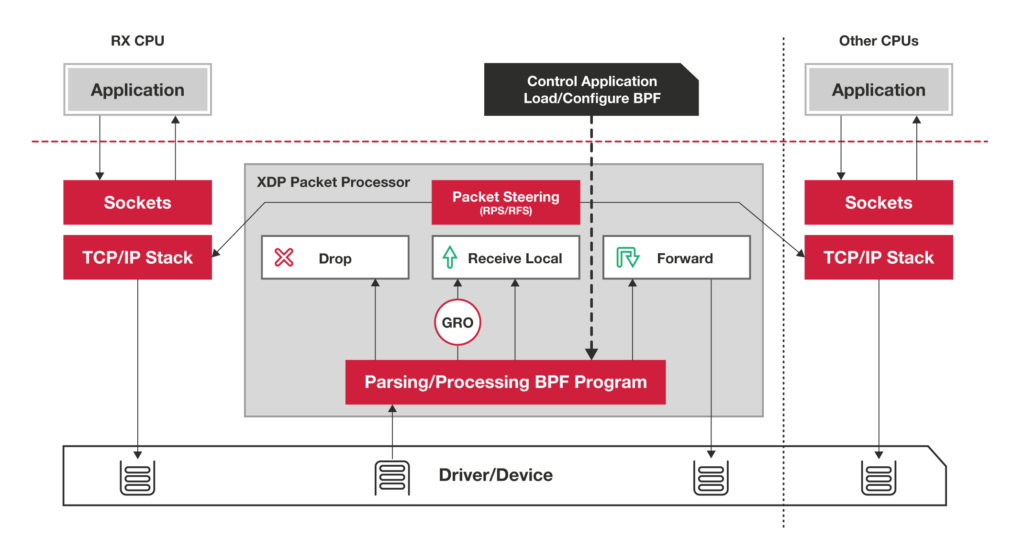
\includegraphics[width=14.5cm]{archivos/img/teoria/xdp-packet-processing.png}
    \caption{Procesamiento de paquetes con XDP}
    \label{fig:xdp_codes}
\end{figure}

\subsection{Limitaciones con \glsentryshort{xdp}}

En esta subsección se indicarán todas las limitaciones que se pueden encontrar a la hora de trabajar con la tecnología \gls{xdp}, además de ciertos detalles que hayan parecido limitaciones aunque sean características de la propia tecnología en favor de ofrecer más seguridad.

\subsubsection{Accesos a memoria y comprobación de limites}

El acceso a los paquetes se hará de modo directo a la memoria, sabiendo que el verificador se asegurará de que dichos accesos sean seguros. Sin embargo, hacer esto en tiempo de ejecución para cada acceso a memoria resultaría en una sobrecarga de rendimiento significativa. Por lo tanto, lo que el verificador hace es comprobar que el programa \gls{xdp} hace su propia comprobación de límites, en su propia lógica \cite{xdp1}. Por ejemplo, si con un programa se están parseando cabeceras Ethernet se haría la comprobación de limites indicada en el bloque \ref{code:xdp_lim}.
%code 
\begin{lstlisting}[language=C, style=C-color, caption={Comprobación de limites en XDP},label=code:xdp_lim]
 SEC("xdp_prog")
 int xdp_ether_parser(struct xdp_md *ctx){
 
	 void *data_end = (void *)(long)ctx->data_end;
	 void *data = (void *)(long)ctx->data;
     int hdrsize = sizeof(struct ethhdr);
    
     /*  Comprobación de limites */
     if (data + hdrsize > data_end)
		 return -1;
		
	 return XDP_PASS;
 }
\end{lstlisting}
\vspace{0.2cm}

En el caso de que se manejen más tipos de cabeceras posteriormente, habría que hacer también comprobaciones de límites con los distintos tipos de cabeceras. De forma general, las definiciones de los parsers se suelen definir aparte como funciones \textit{inline} y  se llaman desde el propio programa \gls{xdp} para hacer el código más legible. \\
\par

Cuando el verificador realiza su análisis estático en tiempo de carga, rastreará todas las direcciones de memoria utilizadas por el programa, y buscará comparaciones con el puntero data-end, el cual será puesto al final del paquete en tiempo de ejecución. En el momento que el verificador crea que puede darse un acceso indebido, descartará el programa \gls{xdp}.


\subsubsection{Bucles y funciones inline}

Puesto que XDP se puede ver como un \textit{framework} \gls{bpf}, también comparte sus limitaciones como son las limitaciones de llamadas a funciones y los bucles. Por ello, muchas de las funciones que se van a desarrollar en los programas \gls{xdp} necesitarán ser de un carácter \textit{inline} ( \texttt{\_\_always\_inline}) para que así el compilador las sustituya tal cual en código.\\
\par
De esta forma se consigue una mejora de rendimiento, ya que no hay que hacer una llamada a una función con todo lo que ello conlleva (Cambio de contexto, salvado de registros, incremento del PC), y se consigue evitar las limitaciones de llamadas a funciones del verificador \cite{xdp2}.\\
\par

En cuanto a la limitación de los bucles, \gls{bpf} no soporta los bucles, por lo que se deberá desenrollar los bucles. Pero, ¿Qué significa desenrollar un bucle? Atendiendo al bloque \ref{code:xdp_loops} podemos hacernos una idea. 

%code 
\begin{lstlisting}[language=C, style=C-color, caption={Loops Unrolling},label=code:xdp_loops]

    #pragma unroll
    for ( int j = 0; j < 4 ; j++)
     printf("Contador %d \n", j);
    
    
    // Si lo desenrollamos, quedaría así:
    printf("Contador %d \n", 0);
    printf("Contador %d \n", 1);
    printf("Contador %d \n", 2);
    printf("Contador %d \n", 3);

\end{lstlisting}
\vspace{0.5cm}

Para conseguir esto debemos añadir la siguiente declaración antes del bucle \textit{pragma unroll}. Esta declaración solo es válida cuando el numero de iteraciones del bucle es conocida en tiempo de compilación y no supera el numero máximo de instrucciones que admite el verificador del Kernel (4096) \cite{xdp1}.



%%%%%%%%%%%%%%%%%%%%%%%%%%%%%%%%%%%%%%%%%%%%%%%%%%%%%%%%%%%%%%%%%%%%%%%%%%%%%%%%%%%%%%%%%%%%%%%%%%%%%

\newpage
\section{Linux Networking}
\label{linuxNetworking}

En esta sección se van a recoger todos los conceptos y herramientas que se engloben en la parte de \textit{Networking} de Linux y se crean fundamentales en el desarrollo de este proyecto.  



%%%%%%%%%%%%%%%%%%%%%%%%%%%%%%%%%%%%%%%%%%%%%%%%%%%%%%%%%%%%%%%%%%%%%%%%%%%%%%%%%%%%%%%%%%

\subsection{Estructura \texttt{sk\_buff}}
\label{linuxNetworking_skbuff}

Se puede afirmar que  esta estructura es una de las más importantes de todo el Kernel de Linux en cuanto a la parte de \textit{Networking} se refiere. Esta estructura representa las cabeceras o información de control para los datos que se van a enviar o para aquellos que se acaban de recibir. Dicha estructura se encuentra definida en el siguiente archivo de cabecera \texttt{<include/linux/skbuff.h>}, y contiene campos de todo tipo, para así tratar de ser una estructura ``todo terreno" que tenga una gran versatilidad. Por ello, se puede llegar a entender que \gls{xdp} no haga uso de esta estructura, ya que habría que hacer una reserva de memoria por cada paquete recibido y esto consumiría bastante tiempo viéndolo a gran escala, dadas las dimensiones de la estructura.\\
\par

Esta estructura es usada por bastantes capas de la pila de protocolos del Kernel, y muchas veces la misma estructura es reutilizada de una capa hacia otra. Por ejemplo, cuando se genera una paquete TCP se añaden las cabeceras de la capa de transporte al payload,  acto seguido se le pasa a la capa de red, IPv4 - IPv6. En esta capa se deben añadir de igual manera sus cabeceras, por ello la estructura sk\_buff que gobierna dicho paquete tendrá que iniciar un proceso de adicción de cabeceras. Este proceso se lleva a cabo haciendo reservas de memoria en el \textit{buffer} gestionado por la estructura, llamando a la función \texttt{skb\_reserve}. Una vez que se tiene reservada memoria para las nuevas cabeceras éstas se copian, se actualizan los punteros de la estructura a las nuevas posiciones de inicio de paquete, y se delega la estructura \textit{stack} de red abajo.\\
\par

 Podría surgir la siguiente pregunta, ¿Cuando llega un paquete qué ocurre? En primera instancia se creía que las cabeceras iban siendo eliminadas del paquete como si de una pila se tratase, cada capa que a travesaba del \textit{stack} de red iba haciendo un \textit{pop-out} de una cabecera. El funcionamiento sin embargo, se lleva a cabo con esta estructura, y no se opera como una pila haciendo \textit{relloc} eliminado capas, sino que en realidad se va moviendo un puntero que apunta al \textit{payload} y  a la información de control según en la capa del \textit{stack} de red en el que se encuentre.\\
\par

Por ejemplo, si el paquete se encuentra en  la capa dos, el puntero de datos apuntaría a las cabeceras de capa dos. Una vez que estas se han parseado, y se pasa el paquete a la capa tres, el puntero se desplazaría a las cabeceras de capa tres. De esta manera el procesamiento de los paquetes supone menos ciclos de CPU, y se consigue un mejor rendimiento ya que no es necesario hacer un \texttt{realloc} con la nueva información ``útil" del paquete.\\
\par


Como ya se ha explicado, esta estructura juega un papel fundamental en el control de cabeceras, pero es igual de importante en el control de colas. Generalmente las colas se organizan en una lista doblemente enlazada, como toda lista doblemente enlazada elemento de la lista tiene un puntero que apunta al siguiente elemento y otro puntero que apunta al elemento anterior de la lista. Pero, una característica especial de esta estructura, es que cada estructura \texttt{sk\_buff} debe ser capaz de encontrar la cabeza de toda la lista rápidamente, de esta forma hace la lista mucho más accesible. Por ello, cada elemento de lista tiene un puntero a una estructura del tipo \texttt{sk\_buff\_head}, la cual estará siempre al principio de la lista. La definición de esta estructura \texttt{sk\_buff\_head} es la siguiente.

% code 
\begin{lstlisting}[language=C, style=C-color, caption={Estructura sk\_buff\_head},label=code:linuxNet_skbuffhead]
    struct sk_buff_head {
    	/* These two members must be first. */
    	struct sk_buff	*next;
    	struct sk_buff	*prev;
    
    	__u32		qlen;
    	spinlock_t	lock;
    };
\end{lstlisting}
\vspace{0.5cm}

El elemento \texttt{lock} se utiliza como cerrojo para prevenir accesos simultáneos a la cola, será un atributo crucial para lograr la atomicidad en la operaciones relativas a la cola. En cuanto al elemento \texttt{next} y \texttt{prev} sirven como elementos para recorrer la cola apuntando estos al primer buffer y al ultimo de ellos. Al contener estos elementos, \texttt{next} y \texttt{prev}, la estructura \texttt{sk\_buff\_head} es completamente compatible en la lista doblemente enlazada, ya que se puede recorrer la cola desde el primer \textit{item} sin problemas. Por último, el elemento \texttt{qlen} es para llevar el número de elementos que hay en la cola en un momento dado.\\
\par

%foto
\begin{figure}[ht]
    \centering
    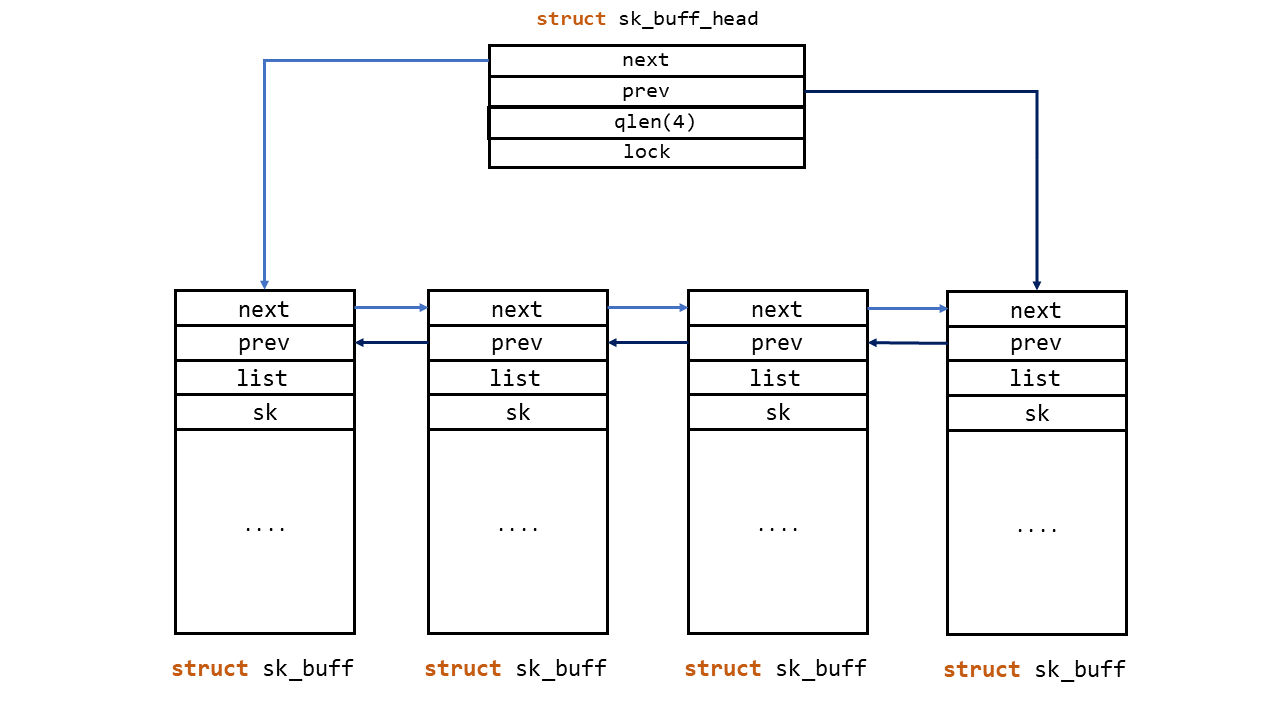
\includegraphics[width=16cm]{archivos/img/teoria/sk_buff_queue.png}
    \caption{Sistema de colas doblemente enlazada}
    \label{fig:linuxNet_skbuff1}
\end{figure}

Por claridad en la figura \ref{fig:linuxNet_skbuff1} no se ha dibujado el enlace de cada elemento de la lista hacia la cabeza de la misma. Pero recordemos que no es una simple lista enlazada, cada elemento de lista tiene un puntero que apunta al primer elemento de la lista, con su parámetro \texttt{list}.\\
\par
Muchos campos de la estructura resultan muy familiares, ya que con \gls{xdp} se tiene que replicar su funcionalidad al no poder disponer de ellos. Pero hay campos en las dos estructuras que son constantes; estos son los punteros que apuntan a posicionas clave del paquete en  memoria.\\
\par

%foto
\begin{figure}[ht]
    \centering
    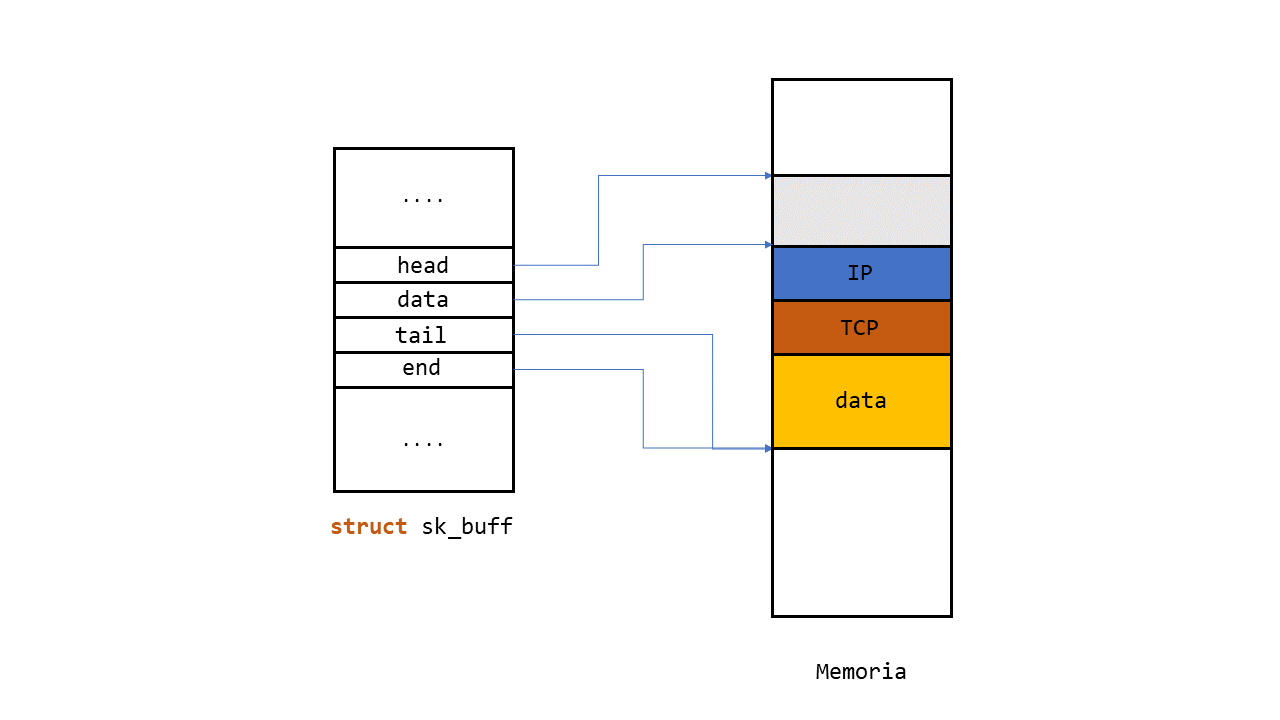
\includegraphics[width=16cm]{archivos/img/teoria/sk_buff.png}
    \caption{Punteros de la estructura sk\_buff}
    \label{fig:linuxNet_skbuff2}
\end{figure}

Estos cuatro punteros a memoria son de utilidad cuando se tiene que llevar a cabo una reserva de memoria para añadir una nueva cabecera. El puntero \texttt{head} siempre apuntará al principio de la posición de memoria reservada en primera instancia, el puntero data siempre apuntará al principio del paquete, por lo que si queremos superponer una cabecera sobre otra simplemente tendremos que reservar la memoria suficiente entre ambos punteros. En cuanto a los punteros, \texttt{tail} y \texttt{end} son útiles para añadir información de control al final del paquete, como por ejemplo el CRC de Ethernet.\\
\par

Esta estructura tiene muchísimas aplicaciones y usos en el Kernel de Linux. En nuestro caso, está estructura está relacionada con el proyecto, por el hecho de que numerosos \textit{helpers} \gls{bpf} hacen uso de ella, pero con \gls{xdp} no podremos al disponer de ella. Por ello, se tendrán que plantear soluciones a la ausencia de funcionalidades por los \textit{helpers} \gls{bpf}, como por ejemplo clonar paquetes, muy útil para difundir paquetes por toda la red o \textit{broadcast}.



%%%%%%%%%%%%%%%%%%%%%%%%%%%%%%%%%%%%%%%%%%%%%%%%%%%%%%%%%%%%%%%%%%%%%%%%%%%%%%%%%%%%%%%%%%

\subsection{Herramienta \texttt{TC}}


\gls{tc}, es un programa de espacio de usuario el cual es la pieza fundamental de la \gls{qos} en el Kernel de Linux. Muchas de sus funcionalidades se pueden resumir en cuatro puntos:

\begin{itemize}
    \item \textsc{SHAPING}
    \item \textsc{SCHEDULING}
    \item \textsc{POLICING}
    \item \textsc{DROPPING}
\end{itemize}

 Según su \textit{man-page}\footnote{\url{https://man7.org/linux/man-pages/man8/tc.8.html}}, el procesamiento del trafico para conseguir dichas funcionalidades, se lleva a cabo con tres tipos de objetos: \textbf{qdiscs}, \textbf{classes} y \textbf{filters}.

\subsubsection{Qdiscs}

El objeto \gls{qdics}, disciplina de cola, es un concepto básico en el Networking de Linux que indica el orden en que los miembros de la cola, en este caso paquetes, se seleccionan para el servicio. Por ejemplo, en un momento dado puede que una herramienta de espacio de usuario requiera de transmitir un paquete, dicho paquete será entregado al \textit{stack} de red, llegando en última instancia a la interfaz de red por la cual va a ser transmitido. En ese momento el paquete se encontrará encolado en una cola de a la espera de ser trasnmitido, estas colas estarán regidas por un \gls{qdics}. El \gls{qdics} por defecto es un pfifo, es un puro \textit{first-in}, \textit{first-out} con limitación en el tamaño de cola en número de paquetes.


\subsubsection{Classes}

La clases se podrían ver como una sub-\gls{qdics} de una \gls{qdics}. Una clase puede contener a su vez otra clase, o más clases, pudiendo conformar sistemas de \gls{qos} en detalle, véase la figura \ref{fig:linuxNet_tc}. Cuando los paquetes son recibidos en una cola administrada por un \gls{qdics}, estos pueden ser encolados en base a las características del paquete en otras colas,  gestionadas por otras clases. Esto permite por ejemplo, priorizar el envío de datos de una aplicación sobre otra. Para ello, los paquetes de ambas aplicaciones se clasificarán en distintas clases, dándole más prioridad a una clase sobre la otra, asignándole más recursos de transmisión y recepción.

%foto
\begin{figure}[ht]
    \centering
    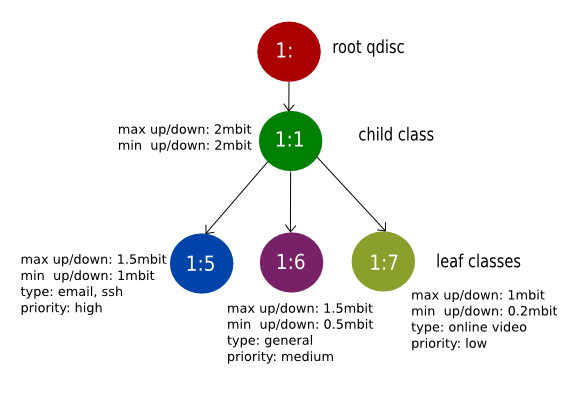
\includegraphics[width=8cm]{archivos/img/teoria/tc_qdisc_example_implementation.png}
    \caption{Sistema de QoS implementado con distintas clases \cite{qdiscs}}
    \label{fig:linuxNet_tc}
\end{figure}

\subsubsection{Filters}

Un filtro es usado para determinar con qué clase debe ser encolado el paquete. Para ello, el paquete siempre debe ser clasificado con una clase determinada. Varios tipos de filtros se pueden utilizar para clasificar los paquetes, pero en este caso será de interés el tipo de filtro \gls{bpf}\footnote{\url{https://man7.org/linux/man-pages/man8/tc-bpf.8.html}}, los cuales permiten anclar un \textit{bytecode} \gls{bpf}. Estos filtros se utilizarán para cargar programas \gls{bpf} que trabajarán en conjunto con \gls{xdp} con la finalidad de lograr el Broadcast. Esto es así, ya que en el \gls{tc} ya se hace uso de la estructura \texttt{sk\_buff} (Ir a \ref{linuxNetworking_skbuff}), por lo que ciertos \textit{helpers} \gls{bpf} para clonar paquetes podrán ser utilizados por \textit{bytecode} anclado en el filtro.


%%%%%%%%%%%%%%%%%%%%%%%%%%%%%%%%%%%%%%%%%%%%%%%%%%%%%%%%%%%%%%%%%%%%%%%%%%%%%%%%%%%%%%%%%%

\subsection{Namespaces}
\label{namespaces}
Una \textit{Namespace} se utiliza para aislar un recurso del sistema en una abstracción que hace  creer a los procesos dentro de dicha \textit{Namespace} que tienen su propia instancia del recurso en cuestión aislada del sistema real.  Los cambios realizados sobre recursos aislados del sistema, son solo visibles para procesos que son pertenecientes a la \textit{Namespace}, pero son invisibles para otros procesos pertenecientes al sistema o a otra \textit{Namespace}.\\
\par
Hay muchos tipos de \textit{Namespaces}, en la tabla \ref{tab:linux_ns} se pueden apreciar todos los tipos que existen a día de hoy. El uso de todos estos tipos de \textit{Namespaces} puede ser muy variado, pero el más importante de todos ellos son los contenedores. Los contenedores son elementos para correr aplicaciones, o herraminetas en un entorno aislado del sistema. A día de hoy, los contenedores más utilizados son los de Docker\footnote{\url{https://www.docker.com/}}, pero, ¿Realmente que hace Docker, qué es Docker?\\
\par

Docker se vale de las bondades del Kernel de Linux para aislar recursos y con esto conformar contenedores. Éste hará uso de las APIs suministradas por el Kernel para crear y destruir a conveniencia las distintas \textit{Namespaces}. Por lo que, Docker en verdad simplemente es un envoltorio de las llamadas al sistema para gestionar \textit{Namespaces}. Docker además, provee de distintos aspectos al usuario como \textit{copy-on-write}, o una configuración en modo \textit{bridge} hacia el exterior, pero en el fondo es 
un mero \textit{wrapper} para la gestión de las \textit{Namespaces} con la finalidad de implementar contenedores. 

\begin{table}[ht]
\centering
\resizebox{\textwidth}{!}{%
\begin{tabular}{|l|l|}
\hline
\rowcolor[HTML]{EFEFEF} 
\multicolumn{1}{|c|}{\cellcolor[HTML]{EFEFEF}{\color[HTML]{24292E} \textbf{Tipo de Namespace}}} & \multicolumn{1}{c|}{\cellcolor[HTML]{EFEFEF}{\color[HTML]{24292E} \textbf{Descripción}}}                                                                                                                                                     \\ \hline
\textbf{Cgroup}                                                                                          & \begin{tabular}[c]{@{}l@{}}Namespace utilizada generalmente para establecer unos limites de recursos,  por ejemplo, \\ CPU, memoria, lecturas y escrituras a disco, de todos los procesos que corran dentro de dicha Namespace.\end{tabular} \\ \hline
Time                                                                                            & Namespace para establecer una hora del sistema diferente a la del sistema.                                                                                                                                                                   \\ \hline
\textbf{Network}                                                                                         & Namespace utilizada para tener una replica aislada del stack de red del sistema, dentro del propio sistema.                                                                                                                                  \\ \hline
\textbf{User}                                                                                            & Namespace utilizada para tener aislados a un grupo de usuarios.                                                                                                                                                                              \\ \hline
\textbf{PID}                                                                                             & Namespace utilizada para tener identificadores de proceso independientes de otras namespaces.                                                                                                                                                \\ \hline
\textbf{IPC}                                                                                             & Namespace utilizada para aislar los mecanismos de comunicación entre procesos.                                                                                                                                                               \\ \hline
\textbf{Uts}                                                                                             & Namespace utilizada para establecer un nombre de Host y nombre de dominio diferentes de los establecidos en el sistema                                                                                                                       \\ \hline
\textbf{Mount}                                                                                           & Namespace utilizada para aislar los puntos de montaje en el sistema de archivos.                                                                                                                                                             \\ \hline
\end{tabular}%
}
\caption{Resumen de los tipos de Namespaces en el Kernel de Linux}
\label{tab:linux_ns}
\end{table}

\subsubsection{Persistencia de las Namespaces}

Atendiendo a la \textit{man-page} \cite{ns} sobre \textit{Namespaces}, es importante señalar que las \textit{Namespaces} tienen una vida finita. La vida finita de la \textit{Namespace} dependerá de si la \textit{Namespace} en cuestión está referenciada, por lo que éstas vivirán siempre y cuando estén referenciadas, cuando dejen de estarlo serán destruidas.\\
\par
Este concepto de vida finita, será útil entenderlo para tener una mejor comprensión sobre el funcionamiento interno de Mininet ó Mininet-WiFI, los cuales se valen de estos conceptos para ahorrarse operaciones y ganar en rendimiento.  Una Namespace a día de hoy puede ser referenciada de tres maneras distintas:\\

\begin{itemize}
    \item Siempre y cuando haya un proceso corriendo dentro de esta \textit{Namespace}.
    \item Siempre que haya abierto un descriptor de archivo al fichero identificativo de la \textit{Namespace} (\texttt{/proc/{pid}/ns/{tipo\_namespace}}).
    \item Siempre que exista un \textit{bind-mount} del fichero (\texttt{/proc/{pid}/ns/{tipo\_namespace}}) de la \textit{Namespace} en cuestión.
\end{itemize}

Si ninguna de estas condiciones se cumple, la \textit{Namespace} en cuestión es eliminada automáticamente por el Kernel. Si se tratase de una \textit{Network Namespace}, aquellas interfaces que se encuentren en la \textit{Namespace} en desaparición volverán a la \textit{Network Namespace} por defecto \cite{ns}.

\subsubsection{Concepto de las Network Namespaces}

Una vez entendido el concepto de \textit{Namespace} en Linux, se introducen las \textit{Network Namespace}, las cuales serán fundamentales para las plataformas donde se probarán los distintos test. Éstas consisten en una replica lógica de \textit{stack} de red que por defecto tiene Linux, replicando rutas, tablas ARP, Iptables e interfaces de red \cite{netns}. \\
\par
 Linux se inicia con un \textit{Network Namespace} por defecto, el espacio \textit{root}, con su tabla de rutas, su tabla ARP,  Iptables e interfaces de red. Pero también es posible crear más \textit{Network Namespace} no predeterminadas,  crear nuevos dispositivos en esos espacios de nombres, o mover un dispositivo existente de un espacio de nombres a otro. \\
 \par
 Para llevar todas estas tareas a cabo, la herramienta más sencilla será \texttt{iproute2} (Ir a Anexo \ref{iproute2}). Esta herramienta, haciendo uso del módulo \texttt{netns}, se podrá gestionar todo en lo relativo a las \textit{Network Namespace} con nombre. Esta coletilla, ``con nombre", atiende a que todas las \textit{Network Namespace} que se gestionen desde \texttt{iproute2} serán persistentes debido a que se realizará un \textit{bind-mount} con el nombre de la \textit{Namespace}, del fichero identificativo de la \textit{Namespace} en cuestión, bajo el directorio \texttt{/var/run/netns} . A continuación, se listan los comandos más frecuentes a la hora de gestionar \textit{Network Namespaces}, se entiende que se ejecutan con permisos de súper usuario.
 
 \begin{lstlisting}[language= bash, style=Consola, caption={Comandos útiles con iproute2 - Netns},label=code:iproute2_ns_use]
    # Para crear una Network Namespace
    ip netns add {nombre netns}
    
    # Para listar las Network Namespaces "con nombre"
    ip netns list
    
    # Para añadir una interfaz a una Network Namespace
     ip netns set {nombre netns} Veth
    
    # Para ejecutar un comando dentro de una Network Namespace
    ip netns exec {nombre netns} {cmd}
    
    # Para eliminar una Network Namespace
    ip netns del {nombre netns}
    
\end{lstlisting}
 
\subsubsection{Métodos de comunicación inter-Namespaces: \glsentryshort{veth}}
\label{linuxVeths}
Las \gls{veth}, son interfaces de Ethernet virtuales creadas como un par de interfaces interconectadas entre si. El modelo funcional es sencillo, los paquetes enviados desde una son recibidos por la otra interfaz de forma directa, bastante parecido al funcionamiento de las \textit{pipes}. Una condición interesante de estas interfaces es que su gestión está asociada, es decir, si se levanta una extremo de la \gls{veth}, la otra también lo hará, si por el contrario se deshabilita o se destruye algún extremo de un par de \gls{veth} el otro extremo también se verá afectado \cite{veth}.\\
\par
Es muy común hacer uso de las \gls{veth} para interconectar \textit{Network Namespaces}, ya que, sabiendo que estas van a estar conectadas de forma directa, se puede utilizar este enlace como pasarela entre dos \textit{Network Namespaces}. De esta forma, se estaría interconectando dos \textit{stacks} independientes de red. La creación y destrucción de este tipo de interfaces se puede apreciar en el bloque \ref{code:iproute2_veth_use}, se recuerda que es necesario permisos de súper usuario.\\

 \begin{lstlisting}[language= bash, style=Consola, caption={Manejo de Veths},label=code:iproute2_veth_use]
    # Crear un par veth
    ip link add {nombre_veth1} type veth peer name {nombre_veth2}
    
    # Si se elimina un extremo, el otro también lo hará
    ip link delete {nombre_veth}
    
\end{lstlisting}
\vspace{0.5cm}

Por lo tanto, se puede llegar al siguiente diagrama básico del funcionamiento de un par de \gls{veth}, las cuales estarán asignadas a una \textit{Network Namespace} distinta.  Como se puede apreciar en la figura \ref{fig:linuxNet_veth}, ambas interfaces están conectadas entre si directamente de forma interna en el propio Kernel. En el caso de que se generen paquetes desde una \textit{Network Namespace} hacia la otra, estos paquetes llegarán desde un extremo de la \gls{veth} directamente al otro extremo de la \gls{veth} a través del Kernel, y en este caso, la \textit{Network Namespace} por defecto no percibirá dicho trafico.\\
\par
Esta condición será de gran utilidad para recrear enlaces entre nodos independientes de red, los nodos se replicarán con \textit{Network Namespaces} y los enlaces con \gls{veth}s. Estos mecanismos serán utilizados por herramientas de emulación de redes como Mininet o Mininet-WiFI, más adelante se destallará. 

\begin{figure}[ht]
    \centering
    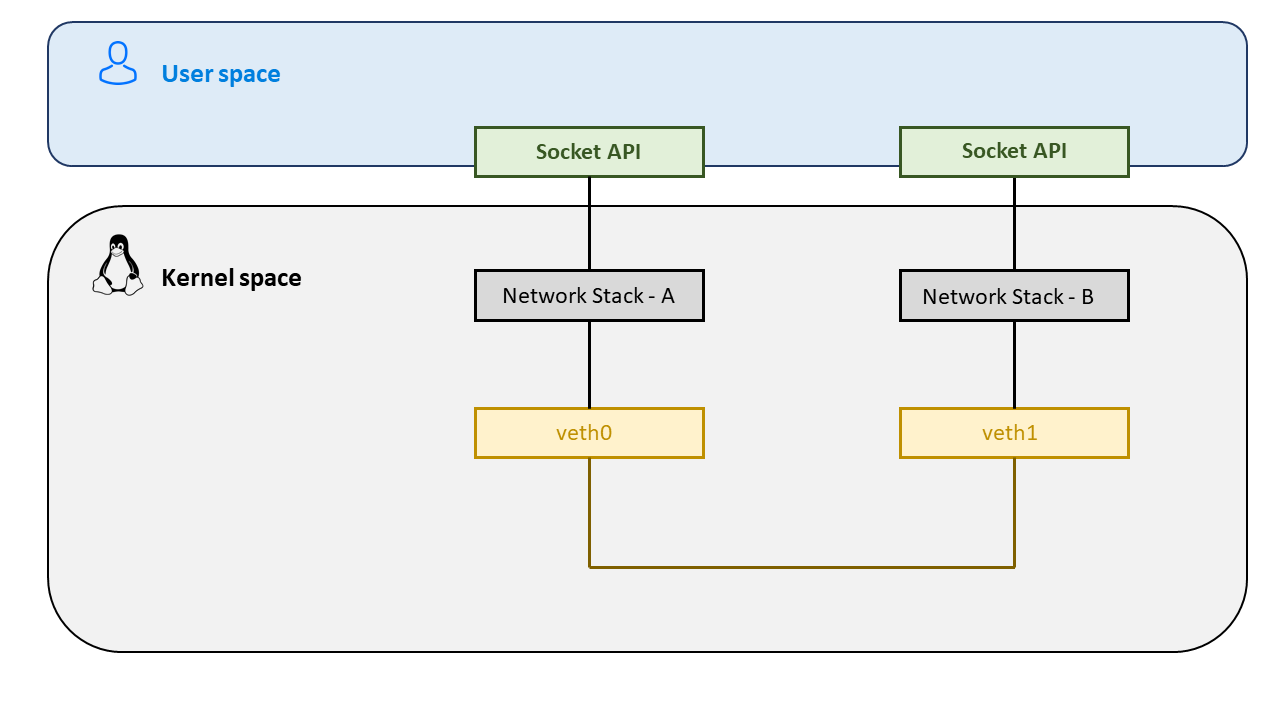
\includegraphics[width=15.5cm]{archivos/img/teoria/user_kernel.png}
    \caption{Enlace entre interfaces Veth separadas en dos Network Namespaces}
    \label{fig:linuxNet_veth}
\end{figure}

%%%%%%%%%%%%%%%%%%%%%%%%%%%%%%%%%%%%%%%%%%%%%%%%%%%%%%%%%%%%%%%%%%%%%%%%%%%%%%%%%%%%%%%%%%%%%%%%%%%%%
\section{Mininet y Mininet-WiFi}
\label{mininet}

En esta sección se cubrirá el marco teórico sobre las principales herramientas de emulación utilizadas en este proyecto. Se indagará en mayor parte Mininet, al ser la herramienta principal desde la cual han nacido otras herramientas de emulación como Mininet-WiFi.\\

\subsection{Mininet}

Mininet es una herramienta que se  utiliza para \textbf{emular} redes,  generalmente del tipo SDN. Con ella se pueden emular host, routers, switches y enlaces en una misma máquina a un bajo coste, pero con la condición de contar con el Kernel de Linux en dicha máquina. Para lograr este cometido se hace uso de una virtualización ``ligera", la cual consiste en hacer uso de las bondades del Kernel de Linux para virtualizar recursos, como son las \textit{Namespaces} (Ir a \ref{namespaces}) \cite{lantz2010network}.\\
\par
En función de las características de cada nodo, se virtualizarán más o menos recursos, y esto dependerá también en el rendimiento de la emulación. Por ejemplo, los nodos del tipo \texttt{Host} en Mininet requieren hacer uso de una \textit{Network Namespace}, de esta forma tendrán su propio \textit{stack} de red y serán completamente independientes\footnote{En la parte de Networking} del sistema y de otros nodos de la red a emular. Sin embargo, por defecto todos los nodos \texttt{Host} comparten sistema de archivos, numeración de PIDs, usuarios, etc. Por lo que técnicamente hablando no están aislados completamente como de un propio \texttt{Host} real se tratase. Esto se debe a que Mininet virtualizará solo aquellos recursos que sean los estrictamente necesarios para llevar a cabo la emulación, de esta forma, se obtiene un mejor rendimiento, y además, permite que máquinas con pocos recursos sean capaces de realizar la emulación \cite{lantz2010network}.\\
\par
En cuanto a la creación de las topologías a emular en Mininet, existen dos vías para hacerlo. La primera es hacer uso de la API escrita en Python para interactuar con las clases de Mininet. Con ella, se podrá conformar toda la topología importando los módulos y clases necesarias de la API para definir dicha topología en un script de Python. La segunda vía es hacer uso de la herramienta \textbf{MiniEdit}, la cual ofrece al usuario una \gls{gui} donde podrá crear la topología emular arrastrando al clickable los distintos nodos de la red. De la misma \gls{gui} además se podrá exportar la topología generada a un fichero (\texttt{*.mn}) para recuperarla más tarde, o a un script en Python (\texttt{*.py}) para levantarla cuando se quiera con el interprete de Python.  Esta herramienta es de gran utilidad para las personas que no saben programar en Python y quieran hacer uso del emulador, por lo que es un gran punto a favor.\\
\par

Por tanto, se podrían resumir los aspectos más fuertes de Mininet en los siguientes puntos:

\begin{itemize}
    \item Es rápido, debido a su condición de diseño con \textit{Namespaces}, más adelante se indicará como se lleva a cabo su gestión.
    \item No consume recursos en exceso, virtualiza únicamente lo necesario, y en el caso que fuera necesario se pueden establecer los recursos máximos para la emulación. 
    \item Ofrece libertad al usuario para crear topologías y escenarios personalizados a través de la API en Python de Mininet. Además, estos escenarios son fácilmente extrapolables\footnote{Los resultados de las pruebas no tienen por que ser exactos en dos máquinas distintas, se emula, no se simula. Por tanto se depende de las condiciones de la máquina donde se vayan a correr las pruebas} a otra máquina, ya que únicamente se debe compartir el script que describe la topología.
\end{itemize}

Al igual que se han indicado los puntos fuertes, se va a indicar la mayor limitación de Mininet. Como ya se comentaba antes Mininet hace uso de una virtualización ``ligera", la cual está sustentada por las \textit{Namespaces} del Kernel de Linux. Es cierto que esta decisión de diseño da muchos beneficios en rendimiento al hacer uso del propio sistema para virtualizar recursos, pero el problema llega cuando este mismo emulador quiere ser exportado a otra plataforma, con un sistema operativo distinto. El cual puede que no soporte el equivalente funcional en ``\textit{Namespaces}", o en caso de hacerlo, su API para hacer uso de ellas sea completamente diferente.


\subsection{Funcionamiento de Mininet}

Se ha introducido anteriormente que Mininet hace uso de \textit{Network Namespaces} como método para virtualizar \textit{stacks} de red independientes entre sí, y así poder emular redes a un coste mínimo. En la figura \ref{fig:mininet_arch}, se puede ver la arquitectura interna de Mininet para una topología compuesta de dos \texttt{Host}, y de un soft-switch conectado por TCP a un controlador remoto.\\
\par
Como se puede apreciar los host están aislados en sus propias \textit{Namespaces}, y en este caso el switch está corriendo en la \textit{Namespace} por defecto (root). El mecanismo para comunicar a los nodos de esta topología como se adelantaba anteriormente son las \gls{veth}s (Ir a \ref{linuxVeths}), las cuales permitirán emular los enlaces entre los distintos nodos de la red.\\


\begin{figure}[ht]
    \centering
    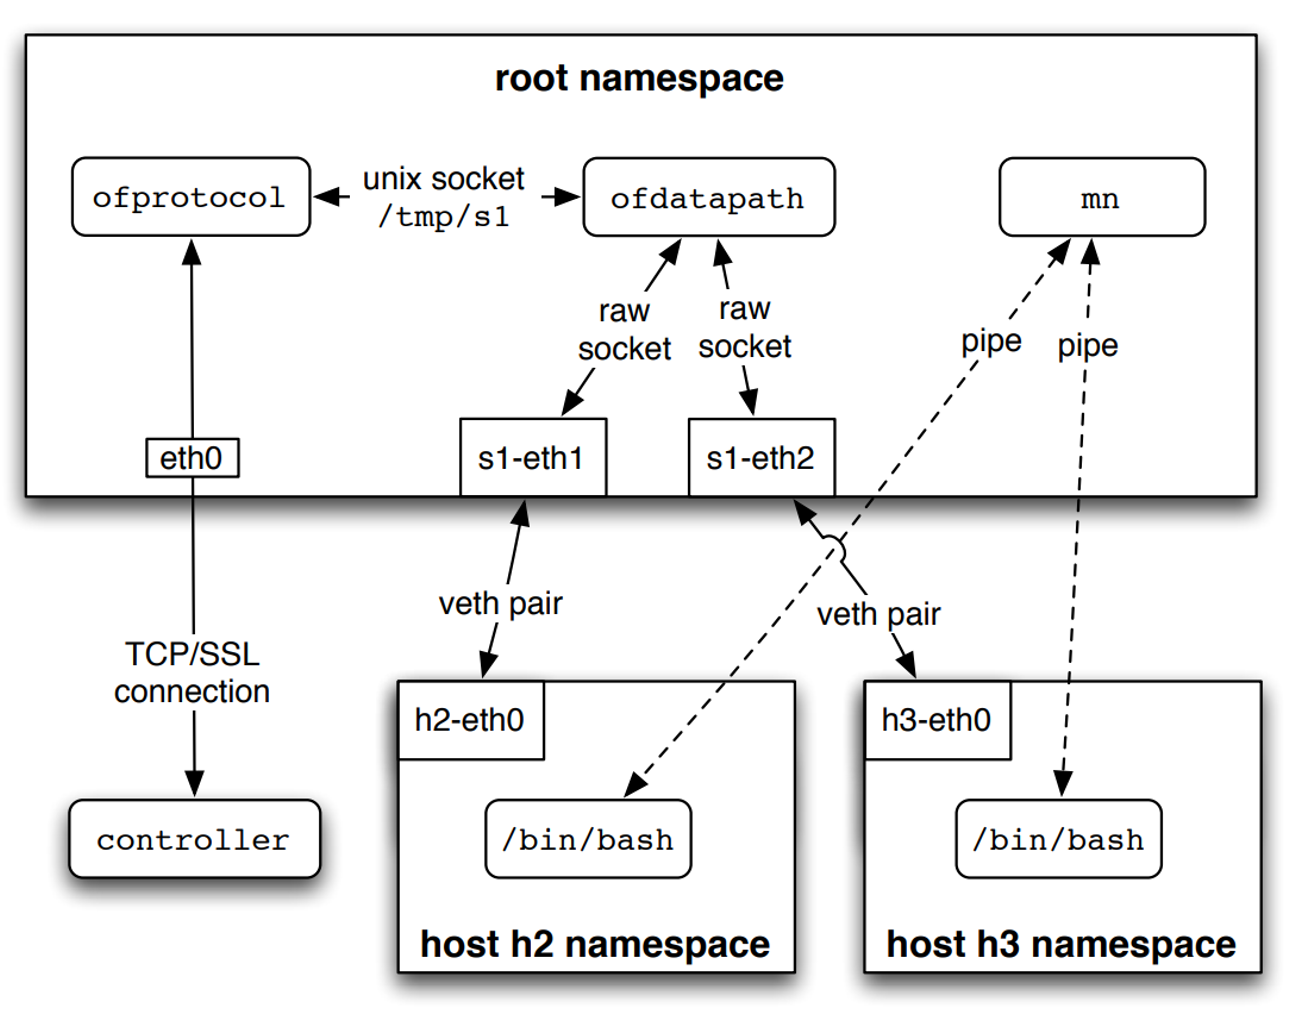
\includegraphics[width=11.5cm]{archivos/img/teoria/mn_arch.png}
    \caption{Arquitectura de Mininet \cite{heller2013reproducible}}
    \label{fig:mininet_arch}
\end{figure}

Una vez expuesta toda la teoría sobre Mininet, podría surgir la siguiente pregunta, ¿Cómo se puede comprobar que realmente hace uso de \textit{Network Namespaces}? Lo primero que se debe hacer es levantar el escenario para que así, Mininet cree las \textit{Network namespaces} que tenga que crear. En este caso, se utilizará la topología expuesta en la figura \ref{fig:mininet_arch}, para levantar dicha topología únicamente se tiene que tener Mininet instalado y seguir los pasos que se indican el bloque \ref{code:scenarioMininet}. 


 \begin{lstlisting}[language= bash, style=Consola, caption={Levantamiento de la topología de ejemplo},label=code:scenarioMininet]
    # Por defecto siempre carga la topología descrita en la figura anterior
    sudo mn
    
\end{lstlisting}
\vspace{0.5cm}

\begin{figure}[ht]
    \centering
    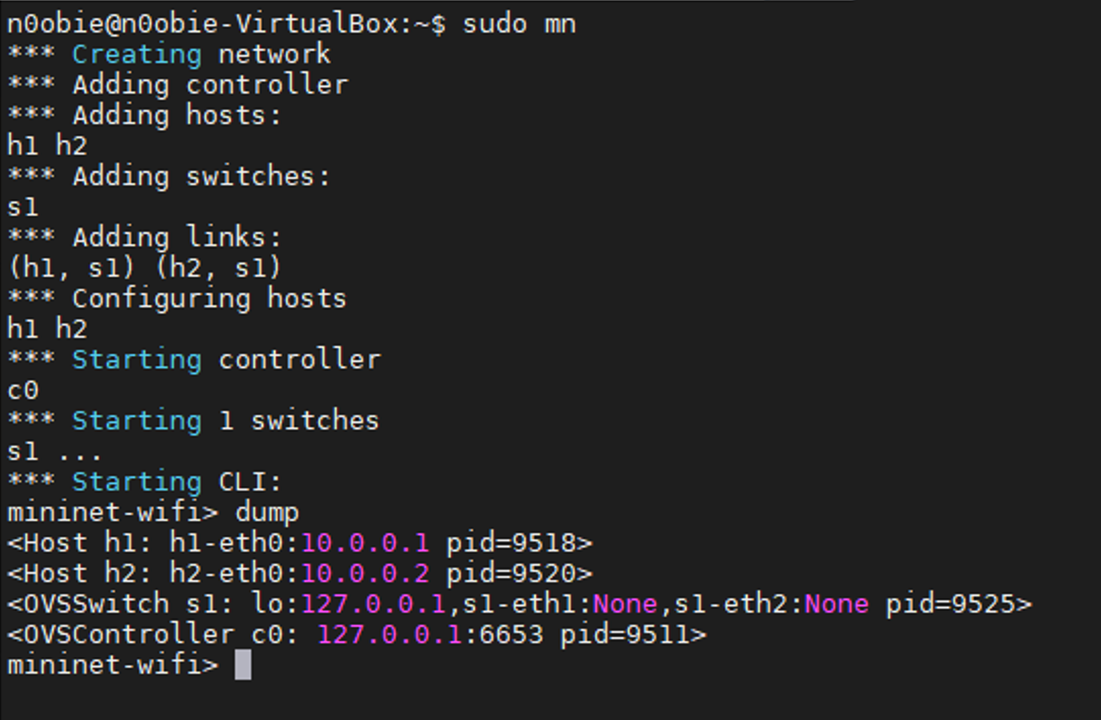
\includegraphics[width=9.5cm]{archivos/img/teoria/mn_01.png}
    \caption{Topología de ejemplo levantada}
    \label{fig:mininet_01}
\end{figure}

Ahora que ya se ha levantado el escenario se debería ser capaces de poder ver si hay \textit{Network Namespaces} en el sistema, para ello se hará uso del \textit{pack} de herramientas iproute2 (Ir a \ref{iproute2}). El comando por excelencia para listar las \textit{Network Namespaces} haciendo uso del módulo \textbf{netns} se puede ver en el bloque \ref{code:MininetNs}.


\begin{lstlisting}[language= bash, style=Consola, caption={Listar Network Namespaces},label=code:MininetNs]
    sudo ip netns list
\end{lstlisting}
\vspace{0.5cm}

\begin{figure}[ht]
    \centering
    
\includegraphics[width=15.5cm]{archivos/img/teoria/mn_02.png}
    \caption{Listado de Network Namespaces existentes en el sistema}
    \label{fig:mininet_02}
\end{figure}

Según se puede apreciar en la figura \ref{fig:mininet_02}, no parece que haya ninguna \textit{Network Namespace} en el sistema, pero entonces, ¿Dónde está el problema? El problema de que el comando \texttt{ip netns list} no arroje información, es que Mininet no está creando el \textit{softlink} requerido para que la herramienta sea capaz de listar las \textit{Network Namespaces}. Atendiendo a la documentación del comando se puede averiguar que dicho comando lee del path \texttt{/var/run/netns/} donde se encuentran todas las \textit{Network Namespaces} con nombre\footnote{Aquellas Netns las cuales se ha hecho un bindmount con su nombre en ese directorio para que persistan aunque no haya ningún proceso corriendo en ellas.}.\\
\par
Como ya se explicó, las \textit{Namespaces} tienen una vida finita, éstas viven siempre y cuando estén referenciadas (Ir a \ref{tab:linux_ns}), por tanto, si ninguna condición de referenciación se cumple, la \textit{Namespace} en cuestión es eliminada.\\
\par
Mininet se encarga de recrear la red emulada, y cuando el usuario termine la emulación, la red emulada debe desaparecer, este proceso debe ser lo más ligero y rápido posible para así ofrecer una mejor experiencia al usuario. La naturaleza del diseño de Mininet incita a pensar que la creación y destrucción de las \textit{Network Namespace} vienen asociadas a la primera condición de refereciación de una \textit{Namespace}. \\
\par
Es decir, no tendría sentido hacer \textit{mounts} ni \textit{softlinks} que a posteriori se deberán eliminar, ya que supondría una carga de trabajo bastante significativa para emulaciones de redes grandes y un aumento del tiempo destinado a la limpieza del sistema una vez que la emulación haya terminado. Además, se debe tener en cuenta que existe una condición que es bastante idónea con las necesidades de Mininet, ya que solo es necesario un proceso corriendo por cada \textit{Network Namespace}, y a la hora de limpiar únicamente se debe terminar con los procesos que sostienen las \textit{Network Namespace}. Cuando ya no haya ningún proceso corriendo en la \textit{Namespace}, y el Kernel se encargará de eliminar las \textit{Namespaces}.\\
\par
Según el razonamiento expuesto, se debería ver varios procesos que son creados a la hora del levantamiento del escenario en Mininet. Estos procesos deberán tener cada uno un fichero de \textit{Network Namespace}, \texttt{/proc/\{pid\}/ns/net}, con un \textit{inode} distinto para aquellos procesos que corren en distintas \textit{Network Namespaces}.\\

\begin{figure}[ht]
    \centering
    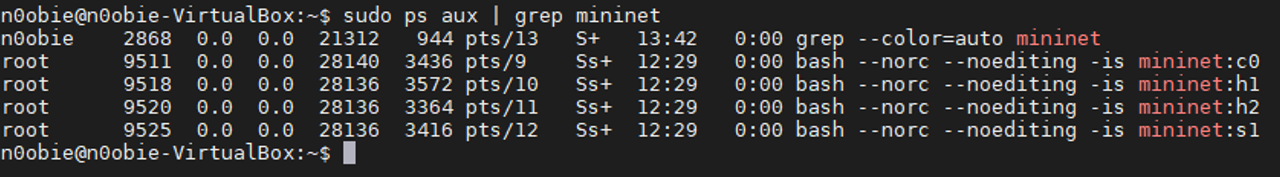
\includegraphics[width=15.5cm]{archivos/img/teoria/mn_03.png}
    \caption{Listado de procesos asociados a Mininet}
    \label{fig:mininet_03}
\end{figure}

Si se inspecciona el fichero \texttt{/proc/\{pid\}/ns/net} para cada proceso indicado en la figura \ref{fig:mininet_03} se podrá ver cuales de ellos están en una \textit{Network Namespace} distinta, en función del valor que tenga el \textit{inode}. Por ejemplo, se va a comprobar los procesos asociados a los \texttt{Host1} y \texttt{Host2}.\\
\par

\begin{figure}[ht]
    \centering
    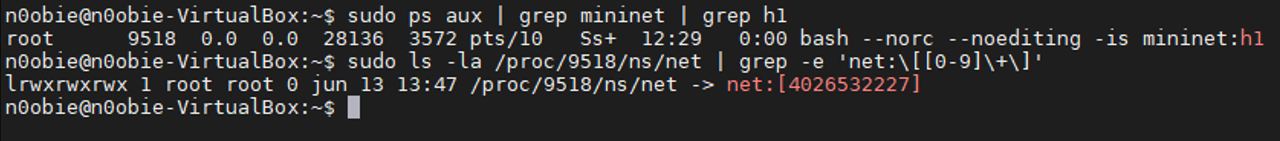
\includegraphics[width=15.5cm]{archivos/img/teoria/mn_04.png}
    \caption{Información relativa al proceso del Host1}
    \label{fig:mininet_04}
\end{figure}

\newpage

\begin{figure}[ht]
    \centering
    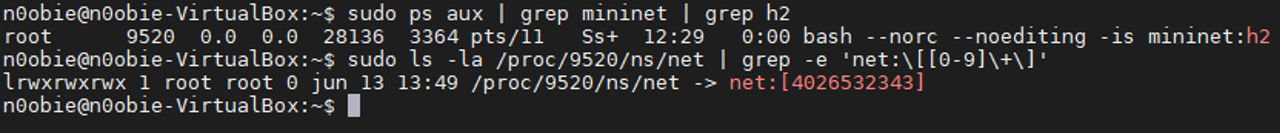
\includegraphics[width=15.5cm]{archivos/img/teoria/mn_05.png}
    \caption{Información relativa al proceso del Host2}
    \label{fig:mininet_05}
\end{figure}

Como se puede ver, \textit{inode} distintos, ficheros distintos, distintas \textit{Network namespaces}. Con esta prueba se puede ver como Mininet hace uso de procesos de bash para sostener las \textit{Network Namespaces} de los nodos que lo requieran. 

\subsection{Mininet CLI}

Mininet incluye una \gls{cli}, la cual puede ser invocada desde el script donde se describe la topología. Dicha \gls{cli}, contiene una gran variedad de comandos, por ejemplo listar la red, tirar enlaces, comprobar el estado de las interfaces, abrir una \textit{xterm} a un nodo, etc. A continuación se indica la tabla \ref{tab:cmdsMininet}, la cual resume todos los comandos existentes a día de hoy, para una explicación de cada uno de ellos en detalle se recomienda seguir esta \href{https://github.com/mininet/mininet/wiki/Introduction-to-Mininet}{\textbf{guía}}\footnote{\url{https://github.com/mininet/mininet/wiki/Introduction-to-Mininet}}.\\
\par

\begin{table}[!ht]
\centering
\begin{tabular}{|c|c|c|c|c|c|}
\hline
\texttt{EOF}      & \texttt{gterm}    & \texttt{links}   & \texttt{pingallfull}  & \texttt{py}     & \texttt{stop}   \\ \hline
\texttt{distance} & \texttt{help}     & \texttt{net}     & \texttt{pingpair}     & \texttt{quit}   & \texttt{switch} \\ \hline
\texttt{dpctl}    & \texttt{intfs}    & \texttt{nodes}   & \texttt{pingpairfull} & \texttt{sh}     & \texttt{time}   \\ \hline
\texttt{dump}     & \texttt{iperf}    & \texttt{noecho}  & \texttt{ports}        & \texttt{source} & \texttt{x}      \\ \hline
\texttt{exit}     & \texttt{iperfudp} & \texttt{pingall} & \texttt{px}           & \texttt{start}  & \texttt{xterm}  \\ \hline
\end{tabular}
\centering
\caption{Resumen comandos existentes en Mininet}
\label{tab:cmdsMininet}
\end{table}


\subsection{Mininet-WiFi}

Mininet-WiFi \cite{7367387} es un emulador de redes inalámbricas diseñado principalmente para trabajar bajo el estándar \texttt{ieee80211}. Esta herramienta nació de Mininet, es decir, es un \textit{fork} de la misma. Por ello, comparten todas las bases sobre virtualización ``ligera" haciendo uso de \textit{Namespaces} y \gls{veth}s, por tanto, todos los scripts de Mininet son compatibles en Mininet-WiFi. \\
\par
Esto es así ya que toda la funcionalidad wireless es un añadido sobre la base que desarrollaron para Mininet. Los desarrolladores de Mininet-WiFi se valieron del subsistema wireless del Kernel de Linux y del módulo mac80211\_hwsim, para conseguir emular las interfaces y el supuesto medio inalámbrico. Para más información sobre esta herramienta se recomienda ir al \textbf{punto} \ref{mn-wifi_bmv2_integration}, donde se hace un análisis profundo sobre las jerarquías de clases añadidas en Mininet-WiFi, como opera internamente y como se comunica con el módulo en el kernel para generar los escenarios inalámbricos.



\subsection{Mininet-IoT}
\label{mininetIoT}

La herramienta Mininet-IoT \cite{mininetIOT} es un emulador de redes de baja capacidad diseñado para trabajar en conjunto bajo el estándar \texttt{ieee802154} y la capa de adaptación 6LoWPAN. Esta herramienta nació de Mininet-WiFi, que a su vez nació de Mininet, por lo que en la práctica, Mininet-IoT comparte todas las técnicas de virtualización ``ligera" de Mininet. Al heredar de Mininet-WiFi y Mininet, todos los scripts para desplegar topologías alámbricas y WiFi son compatibles en Mininet-IoT.  \\
\par

La gran diferencia entre Mininet-IoT y Mininet-WiFi, radica en el módulo que emplean para conseguir emular las interfaces y el supuesto medio inalámbrico. Mininet-WiFi hace uso del módulo mac80211\_hwsim, mientras que Mininet-IoT hace uso del módulo del Kernel mac802154\_hwsim (es necesario tener una versión del Kernel superior a la \texttt{4.18.x} para obtener dicho modulo). Toda la gestión de nodos, interfaces y enlaces es exactamente la misma a la de Mininet-WiFi. Por ello, Ramon Fontes (principal desarrollador de la herramienta), creó una clase agnóstica para gestionar módulos del Kernel en Mininet-WiFi, y migró todo el proyecto de Mininet-IoT a Mininet-WiFi. De esta forma, el mantenimiento del \textit{core} que compartían ambas herramientas se hacía únicamente en un proyecto, y daba la posibilidad al usuario de Mininet-WiFi de establecer enlaces de baja capacidad en sus topologías inalámbricas.  

%%%%%%%%%%%%%%%%%%%%%%%%%%%%%%%%%%%%%%%%%%%%%%%%%%%%%%%%%%%%%%%%%%%%%%%%%%%%%%%%%%%%%%%%%%%%%%%%%%%%%

%\newpage
\section{Contiki-ng}
\label{contikiNG}

Contiki es un sistema operativo enfocado a sensores de baja capacidad. Este sistema operativo fue desarrollado por Adam Dunkels con la ayuda de  Bjorn Gronvall y Thiemo Voigt en el año 2002. Desde entonces hasta los últimos años, el proyecto Contiki  ha involucrado tanto a empresas como a cientos de colaboradores en su repositorio de GitHub\footnote{\url{https://github.com/contiki-os/contiki}}.  Contiki estaba diseñado con el propósito de ofrecer a los nodos de las redes \gls{wsn} un sistema operativo ligero con capacidad de carga y descarga de servicios únicos de forma dinámica \cite{1367266}. \\
\par
El Kernel de Contiki está orientado a eventos, y soporta tareas multi-hilo con requisa. Contiki está escrito en el lenguaje C y ha sido portado a numerosas de arquitecturas de microcontroladores, como el MSP430 de Texas Instruments y derivados. \\
\par

En un sistema que ejecute el sistema operativo de Contiki, éste estará dividido en dos partes claramente diferenciadas según se puede ver en la figura \ref{fig:contikiParts}, el \textit{core} y los programas o servicios cargados. El particionado se lleva a cabo en el momento de la compilación y es independiente de cada target en el que se vaya a desplegar el sistema. El \textit{core} consiste en el propio Kernel, un conjunto de servicios de base (\textit{timers}, \textit{handlers}) , librerías, drivers y el \textit{stack} de comunicación. Los programas o servicios cargados se mapearán en memoria por el propio cargador que tiene el Kernel en tiempo de ejecución.\\
\par


% Foto 
\begin{figure}[ht]
    \centering
    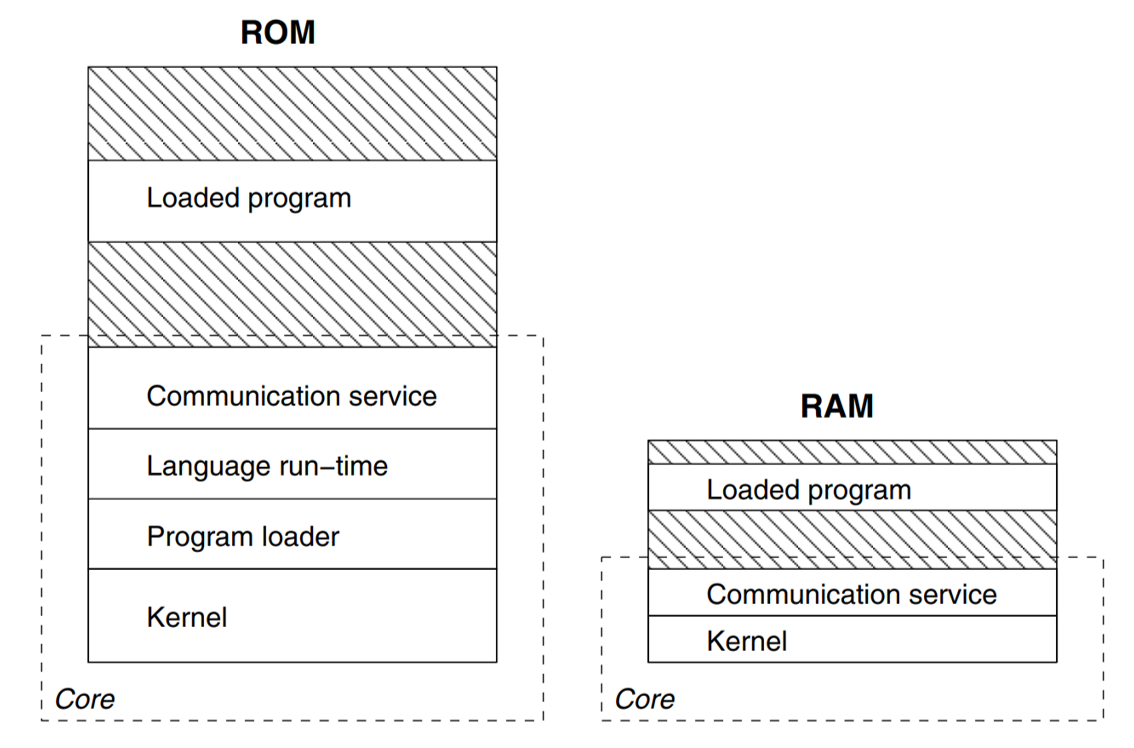
\includegraphics[width=9.5cm]{archivos/img/teoria/contiki.png}
    \caption{Particionado en un sistema con Contiki OS \cite{1367266}}
    \label{fig:contikiParts}
\end{figure}

En los últimos años apareció un nuevo proyecto, \textbf{Contiki-ng} \footnote{\url{https://github.com/contiki-ng/contiki-ng}}, el cual es fork de Contiki OS. Este nuevo proyecto desbancaría a su predecesor bajo el eslogan de ``\textit{Contiki-NG: The OS for Next Generation IoT Devices}". Actualmente toda la comunidad de Contiki está enfocada en este nuevo proyecto, el cual proporciona un \textit{stack} de comunicación más cercano a las RFCs, soporte a protocolos como IPv6/6LoWPAN y 6TiSCH, y por lo que se está haciendo más popular, dar soporte a microcontroladores con la arquitectura ARM \cite{kurniawan2018practical}.
\vspace{0.5cm}


\subsection{Simulador Cooja}

El flujo de trabajo con Contiki o Contiki-ng, dependerá si se va a trabajar sobre hardware real o si se va a simular los programas desarrollados. Cuando se trabaja sobre hardware real, el flujo de trabajo consistirá en la compilación del sistema operativo y de los programas desarrollados con el target donde se vaya a trabajar, generando así un binario el cual se podrá instanciar en el disco del hardware. \\

\par
Si por el contrario se va a simular, se hará uso del simulador llamado Cooja\footnote{\url{https://github.com/contiki-ng/cooja/tree/master}}. Cooja es una simulador escrito en Java que permite simular una serie de motas \gls{iot}. Por tanto, a la hora de simular se podrá ver el comportamiento del programa desarrollado en distintas plataformas. \\
\par

Todo el proceso de compilación del \textit{core} de Contiki y programas desarrollados está integrado en el propio simulador, permitiendo al usuario compilar sus programas hacia distintos tipos de motas. Cada simulación se podrá almacenar en un fichero con la extensión \texttt{*.csc}, los cuales almacenarán todos los datos de la simulación, \textit{seed}, posiciones y tipos de motas en una estructura XML. \\
\par


% % Foto 
% \begin{figure}[ht]
%     \centering
%     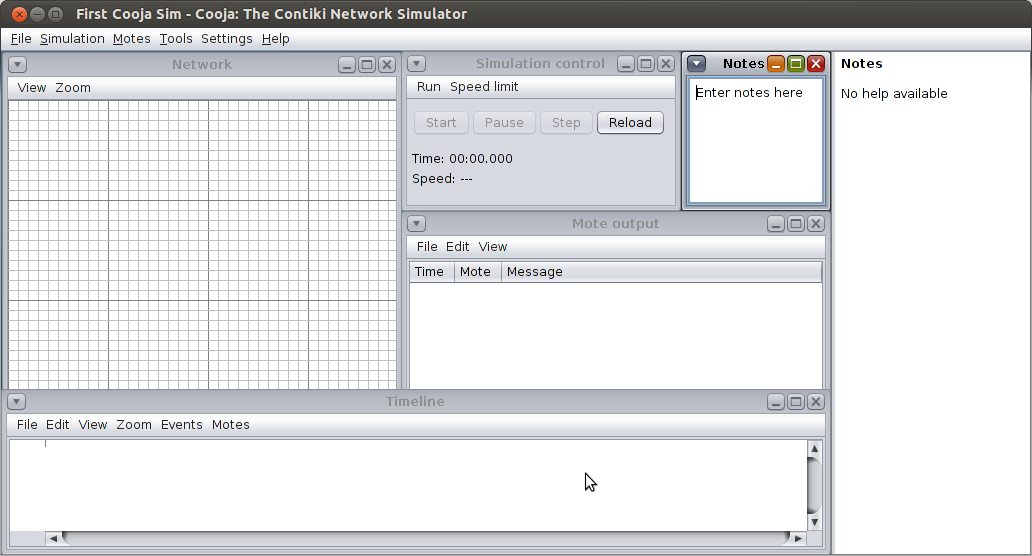
\includegraphics[width=13.5cm]{archivos/img/teoria/cooja.png}
%     \caption{GUI Simulador Cooja \cite{cooja}}
%     \label{fig:cooja}
% \end{figure}

%%%%%%%%%%%%%%%%%%%%%%%%%%%%%%%%%%%%%%%%%%%%%%%%%%%%%%%%%%%%%%%%%%%%%%%%%%%%%%%%%%%%%%%%%%%%%%%%%%%%%

\newpage
\section{Contribuciones en GitHub}
\label{estadoArte_github}


La herramienta GitHub \cite{github2016github} es una plataforma para alojar repositorios de forma remota. En este \gls{tfg}, se hará uso de la herramienta de control de versiones Git\footnote{\url{https://git-scm.com/}}, y de GitHub como plataforma para alojar el código. Pero no se hará un uso exclusivo de la plataforma para almacenar el código desarrollado en el \gls{tfg}, sino que se aprovechará el carácter público del repositorio para ofrecer documentación y ejemplos a todos los usuarios interesados que lo visiten. \\
\par
\begin{itemize}
    \item Enlace al repositorio del \gls{tfg}: \url{https://github.com/davidcawork/TFG} 
\end{itemize}
\vspace{0.5cm}
Todo el proceso de documentación en el repositorio pasa por los ficheros \texttt{README}, los cuales se podrán encontrarán en todos los directorios del repositorio. Estos ficheros suministrarán la información necesaria a los visitantes para poder replicar las pruebas realizadas, y hacer uso del \textit{software} desarrollado. Pero además, se han añadido las explicaciones y  los análisis teóricos necesarios, para que el visitante realmente entienda la naturaleza de las pruebas, que se espera de ellas y que conclusiones se podrán sacar de dichos test.  \\
\par

La finalidad del repositorio por tanto es doble, ya que servirá para almacenar el código, pero también ayudará a divulgar los contenidos de este proyecto. De forma adicional, todos los desarrollos útiles y que pueden aportar en otros repositorios se han ofrecido en forma de contribución vía \textit{pull-request}. A continuación, se en la tabla \ref{tab:githubContr} se indican  todas las contribuciones realizadas.\\
\par

\begin{table}[ht]
\centering
\resizebox{\textwidth}{!}{%
\begin{tabular}{|l|l|}
\hline
\rowcolor[HTML]{EFEFEF} 
\multicolumn{1}{|c|}{\cellcolor[HTML]{EFEFEF}{\color[HTML]{24292E} \textbf{Contribución}}} & \multicolumn{1}{c|}{\cellcolor[HTML]{EFEFEF}{\color[HTML]{24292E} \textbf{Enlace al Pull-Request}}} \\ \hline
Nuevo método de instalación de todas las dependencias del entorno P4                       & \url{https://github.com/p4lang/tutorials/pull/261}                                                        \\ \hline
Corregir documentación del repositorio XDP Tutorial                                        & \url{https://github.com/xdp-project/xdp-tutorial/pull/95}                                               \\ \hline
Integración del BMV2 en Mininet-Wifi                                                       & \url{https://github.com/intrig-unicamp/mininet-wifi/pull/302}                                             \\ \hline
Arreglar interfaz gráfica cuando los APs tienen movilidad                                  & \url{https://github.com/intrig-unicamp/mininet-wifi/pull/229}                                             \\ \hline
Dar soporte de las estaciones Wifi en el comando pingallfull                               & \url{https://github.com/intrig-unicamp/mininet-wifi/pull/230}                                             \\ \hline
\end{tabular}%
}
\caption{Resumen de contribuciones realizadas}
\label{tab:githubContr}
\end{table}

%%%%%%%%%%%%%%%%%%%%%%%%%%%%%%%%%%%%%%%%%%%%%%%%%%%%%%%%%%%%%%%%%%%%%%%%%%%%%%%%%%%%%%%%%%%%%%%%%%%%%
\newpage	
\chapter{Diseño y análisis de casos de uso}
\label{analisisPreimplementacion}

En este capítulo, teniendo en cuenta el marco teórico explicado en el Estado del Arte (Cap. \ref{estadoArte}), se analizará qué funcionalidades básicas deben poder ser implementadas por las distintas tecnologías para definir el \textit{datapath} de los dispositivos \gls{iot}, con el fin de alcanzar los objetivos indicados en la Introducción (Cap. \ref{intro}). \\
\par
Para ello, se diseñarán distintos casos de uso para comparar así las características que ofrecen cada una distintas tecnologías en relación a su  integración de los dispositivos \gls{iot} en entornos \gls{sdn}. De forma adicional, se estudiará sobre que plataformas se desplegarán los casos de uso, asegurándose de que tienen todos los mecanismos necesarios para llevar a cabo las pruebas. 

\section{Funcionalidades básicas}

Como se ha podido ver en el capítulo del Estado del arte (Cap. \ref{estadoArte}), las tecnologías  P4 y \gls{xdp} tienen muchos puntos fuertes, y amabas permiten definir el \textit{datapath} del dispositivo en cuestión. Con \gls{xdp}, obtenemos un gran rendimiento ya que el procesamiento de los paquetes se realiza casi en la propia interfaz, no consume recursos de forma activa, ya que opera de forma reactiva a los paquetes que llegan a la interfaz. Por otro lado, se encuentra la tecnología P4, la cual propone hacer uso de un lenguaje agnóstico del hardware  para definir el datapath. Esto aporta mucha versatilidad a la hora de implementar nuevos protocolos, o nuevas especificaciones de estándares. \\

\par

Teniendo en cuenta estas premisas, se ha decidido plantear una serie de funcionalidades básicas que una hipotética mota \gls{iot} tendría que implementar. Estas funcionalidades se van a recoger en casos de uso, los cuales serán desarrollados con ambas tecnologías (P4 y \gls{xdp}) para poder concluir con cual de ellas es más sencillo/eficiente realizar la integración de los dispositivos \gls{iot} en entornos \gls{sdn}, tal y como se ha definido en el objetivo principal del presente \gls{tfg}. \\
\par

Los casos de uso que se plantean son los siguientes: 

\begin{itemize}
    \item   \textbf{Case01 - Drop}: En este caso de uso se quiere ver si es posible descartar paquetes.
    \item   \textbf{Case02 - Pass}: En este caso de uso se quiere comprobar si es posible dejar pasar los paquetes, sin afectarles el plano de datos programado con la tecnología.
    \item   \textbf{Case03 - Echo server}: Este caso de uso, aunque se desarrollará un servidor el cual contestará todos los \texttt{ECHO-Resquest} que le lleguen, lo que se quiere ver es la facilidad que tenemos con ambas tecnologías de filtrar/parsear paquetes en base a sus cabeceras.
    
    \item   \textbf{Case04 - Layer 3 forwarding}: Con este caso de uso se comprobará qué tan sencillo es reenviar paquetes desde una interfaz a otra del dispositivo. 
    
    \item   \textbf{Case05 - Broadcast}: Por último, con este caso de uso se quería abordar cómo se puede conseguir  la difusión (o broadcast) de un hipotético paquete, es decir, si es posible clonar paquetes con las tecnologías o, en su lugar, crearlos de cero. 
\end{itemize}

Una vez definidas las funcionalidades a desarrollar con ambas tecnologías, se debe decidir sobre qué elementos se van a probar. En el caso de \gls{xdp} es sencillo, ya que como se explicó en el Estado del arte, los programas \gls{xdp} pueden ser cargados en la mayoría de interfaces gestionadas por el Kernel de Linux. \\
\par

%%%%%%%%%%%%%%%%%%%%%%%
% figura XDP process
\begin{figure}[ht]
    \centering
    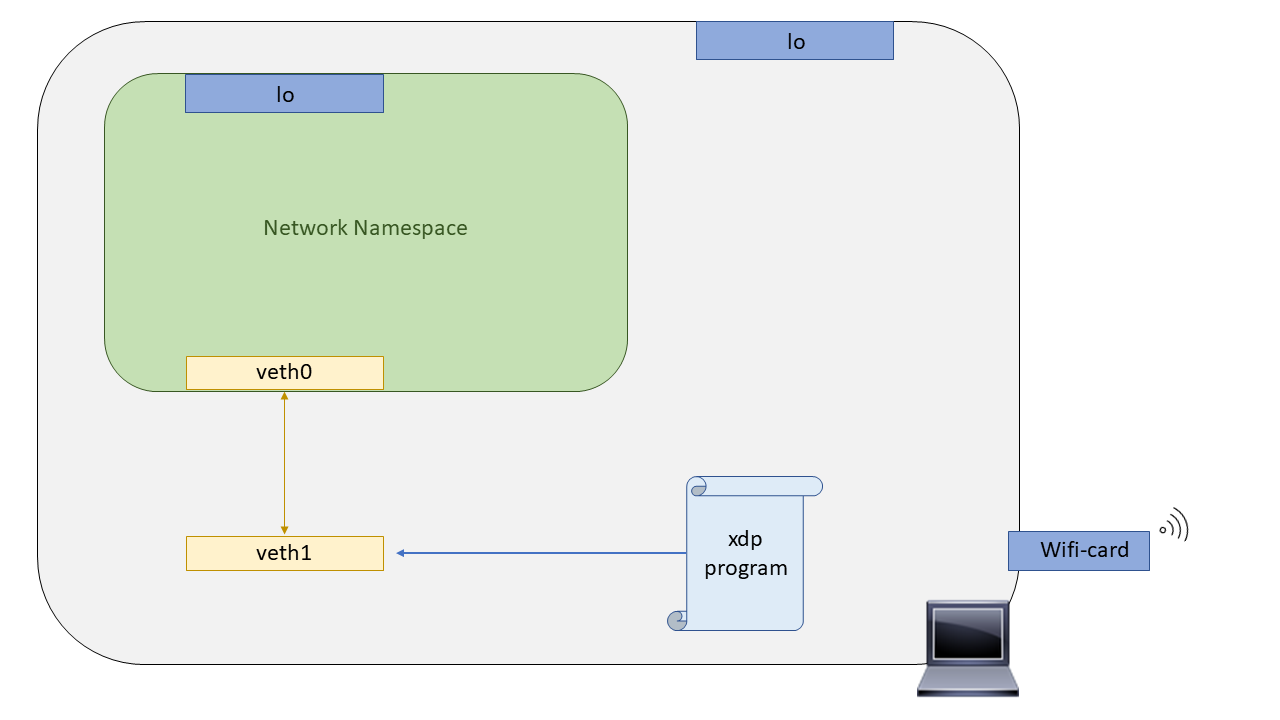
\includegraphics[width=14cm]{archivos/img/analisis/xdp_process.png}
    \caption{Ejemplo de carga de un programa XDP sobre una interfaz Ethernet virtual}
    \label{fig:xdp_process}
\end{figure}
%%%%%%%%%%%%%%%%%%%%%%%


En el caso de los programas P4 sí será necesario hacer uso de un elemento adicional para probar la funcionalidad desarrollada. Dicho elemento es el \gls{bmv2} \cite{p42018behavioral}, un soft-switch\footnote{ Switch virtual que se implementa a nivel de software.} desarrollado con la finalidad de probar código P4. Como se puede apreciar en la figura \ref{fig:p4_process}, el programa P4 una vez compilado se obtendrá un fichero JSON \cite{json} resultante que será el que le indique al \gls{bmv2} qué \textit{datapath} debe implementar.\\
\par

%%%%%%%%%%%%%%%%%%%%%%%
% figura P4 process
\begin{figure}[t]
    \centering
    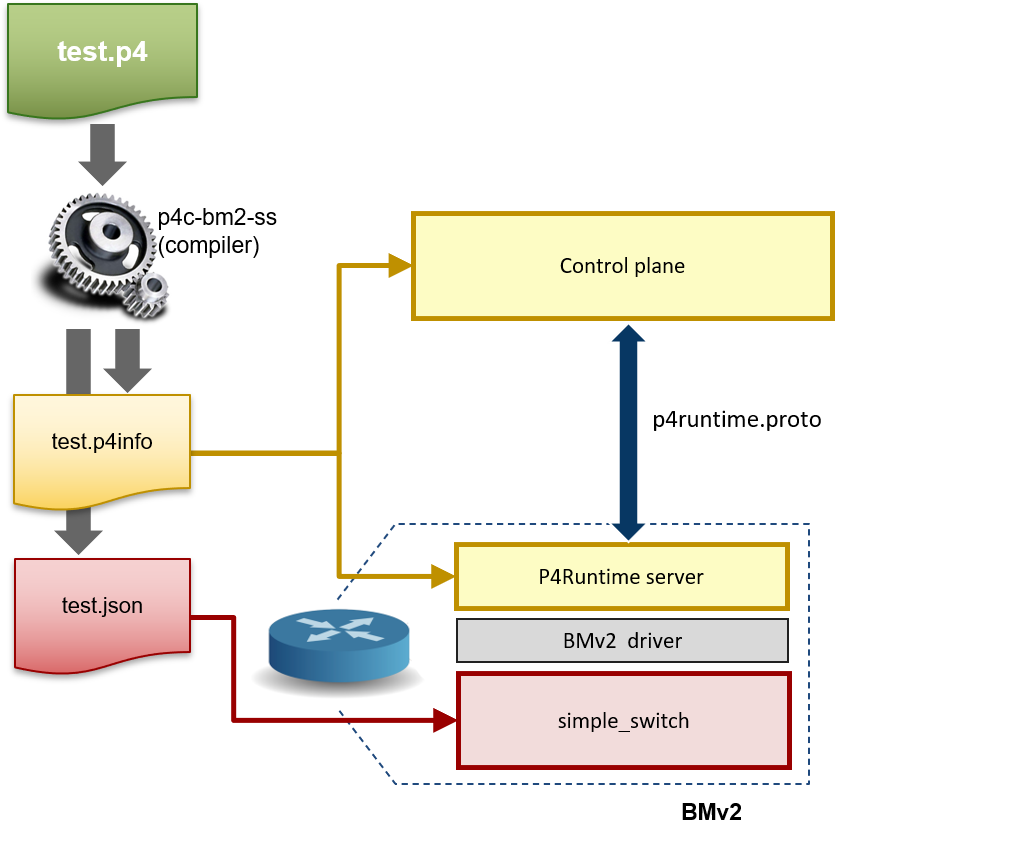
\includegraphics[width=11cm]{archivos/img/analisis/bmv2_process.png}
    \caption{Ejemplo de carga de un programa P4 sobre el BMV2}
    \label{fig:p4_process}
\end{figure}
%%%%%%%%%%%%%%%%%%%%%%%


Atendiendo a los modelos de integración de dispositivos \gls{iot} comentados en la Introducción \ref{sdn_iot_parcial} y \ref{sdn_iot_total}, se van a desarrollar casos de uso tanto en entornos  \textbf{cableados} como para entornos  \textbf{inalámbricos}. La motivación de esta decisión se basa en que, como se puede ver en la figura \ref{sdn_iot_parcial}, habrá dispositivos híbridos \gls{iot} mediadores, los cuales estarán parcialmente conectados al core \gls{sdn} de manera cableada, y de manera inalámbrica con el resto de dispositivos \gls{iot}. Por ello, se estima necesario comprobar el rendimiento de ambas tecnologías en ambos entornos , ya que ciertos dispositivos \gls{iot} en las integraciones parciales pueden ser favorecidos de igual manera. \\
\par

A continuación, se analizará sobre qué plataformas se llevará a cabo la evaluación de las funcionalidades básicas desarrolladas. Se elegirán plataformas para entornos cableados y para entornos  inalámbricos, intentando siempre hacer uso de un número mínimo de ellas para que así las evaluaciones sean lo más homogéneas posibles. 


\section{Plataformas de pruebas alámbricas}

Para evaluar los desarrollos de \gls{xdp} y P4 en entornos  cableados se hará uso del estándar \texttt{ieee8023} (Ethernet), aunque este estándar se diseñó en un principio para operar en redes de carácter local, con el paso de los años la tecnología Ethernet fue avanzando a la par que su popularidad, alcanzando tasas de transmisión de \textit{40 Gbit/s} con el estándar \texttt{ieee8023ba}\footnote{\url{http://www.ieee802.org/3/ba/}}. \\
\par

 Las evaluaciones de los programas \gls{xdp} serán realizadas sobre una plataforma Linux donde se generaran topologías de red conformadas por \textit{Network Namespaces}, para definir los nodos independientes de la red, y de \gls{veth}, para emular los enlaces entre distintos nodos. Todos los escenarios empleados serán suministrados en el repositorio del \gls{tfg} en forma de \textit{shellscript}, indicando al usuario cómo lanzar dicho escenario, y cómo hacer uso del mismo script para limpieza del escenario recreado. Se ha querido hacer uso de \textit{Network Namespaces} como plataforma para validar los desarrollos, ya que es la expresión más básica de emulación de redes en el Kernel de Linux. De esta forma, y debido a la complejidad que supone trabajar con programas \gls{xdp}, se buscaba que la plataforma donde se fueran a evaluar los casos de uso aportase la mínima incertidumbre posible sobre los resultados obtenidos. \\

\par

En cuanto a la plataforma elegida para evaluar los programas P4, se hará uso de Mininet. Como ya se comentó en el Estado del Arte (Cap. \ref{estadoArte}), Mininet es una herramienta para la emulación de topologías de red \gls{sdn}, de la cual nació Mininet-WiFi añadiendo soporte para redes inalámbricas. Se ha elegido Mininet, debido a que el equipo de \textit{p4lang} desarrolló una interfaz\footnote{\url{https://github.com/p4lang/tutorials/tree/master/utils/mininet}} del \gls{bmv2} con dicha herramienta, de esta forma es posible incorporar el soft-switch de referencia para probar código P4, como un tipo de nodo más en Mininet. 
 

\section{Plataformas de pruebas inalámbricas}


Para evaluar los desarrollos de \gls{xdp} y P4 en entornos  inalámbricos se hará uso del estándar \texttt{ieee80211} (WiFi). Se ha elegido dicho estándar cómo un primer paso, debido a que a día de hoy, existen más herramientas y desarrollos que para el estándar \texttt{ieee802154}. El estándar \texttt{ieee80211} es uno de los estándares de redes inalámbricas más populares del mundo recibiendo constantes actualizaciones por parte del \gls{ieee} para mejorar su rendimiento, o dar soporte a nuevas funcionalidades \cite{gast2005802}. Siendo este grupo de trabajo uno de los más activos dentro del proyecto de estandarización del \gls{ieee} de redes de area local (Fig. \ref{fig:ieee802}).  \\
\par

%%%%%%%%%%%%%%%%%%%%%%%
% figura familia 802
\begin{figure}[ht]
    \centering
    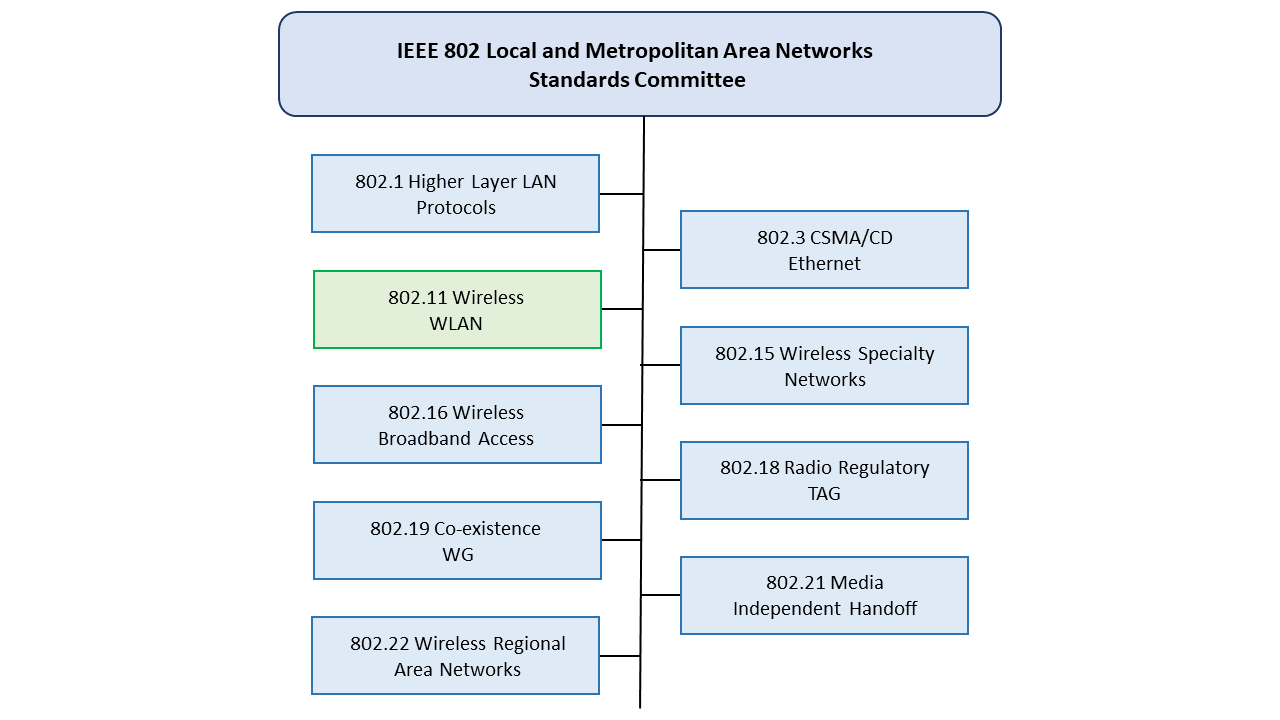
\includegraphics[width=15.5cm]{archivos/img/analisis/802_X_estandares_2.png}
    \caption{Grupos de trabajo IEEE 802}
    \label{fig:ieee802}
\end{figure}
%%%%%%%%%%%%%%%%%%%%%%%


La plataforma que se utilizará para la evaluación de los distintos casos de uso, tanto en \gls{xdp} como en P4, será la misma. Se hizo uso del emulador Mininet-WiFi en lugar del simulador Cooja para evaluar el funcionamiento de ambas tecnologías (XDP y P4) en entornos  inalámbricos. Esto se debe a que para probar ambas tecnologías se requiere de interfaces reales o emuladas donde poder evaluar el funcionamiento de los desarrollos. También se podría haber valorado hacer uso del emulador Mininet-IoT, pero como se menciono en la sección \ref{mininetIoT}, dicha herramienta se integró en Mininet-Wifi como un complemento más. Por lo que, eligiendo a Mininet-WiFi se tiene las nuevas funcionalidades de Mininet-IoT y además, cuenta con mayor madurez al llevar más años en la escena.\\


\par
En los desarrollos \gls{xdp}, el flujo de trabajo consistirá en a levantar la topología en Mininet-WiFi, a través de un script en Python que hará uso de la API de Mininet-WiFi para recrear el escenario, acto seguido se anclará el programa \gls{xdp} en las interfaces del nodo de la red que corresponda. En cuanto a los programas P4, se ha visto que la plataforma no contempla ningún tipo de nodo que de soporte al \gls{bmv2} por lo que será necesario desarrollar previamente una integración del \gls{bmv2} en Mininet-WiFi. Es importante comentar que durante el desarrollo de este \gls{tfg}, el desarrollador principal de Mininet-WiFi, profesor de de la IFBA, Ramon Fontes\footnote{\url{https://github.com/ramonfontes}} empezó de forma paralela una integración de P4 en Mininet-WiFi abriendo un \textit{Issue}\footnote{\url{https://github.com/intrig-unicamp/mininet-wifi/issues/295}} donde mencionaba cómo debía desarrollarse la integración. En dicho \textit{Issue}, se pudieron debatir los detalles de la implementación de los soft-switch P4 en Mininet-WiFi. Más adelante, en el capitulo de desarrollo se expondrá como se abordó la integración, explicando su pre-implementación y desarrollo. \\

\par

El desarrollo de esta integración será vital para el proyecto. Teniendo en cuenta que la evaluación de los programas P4 en entornos inalámbricos dependerá de si se es capaz de embeber el \gls{bmv2} en la arquitectura de Mininet-WiFi. Los pasos propuestos para llevar a cabo la integración son los siguientes:
\vspace{0.5cm}

\begin{itemize}
    \item  Estudio y análisis de la interfaz creada desde el equipo \textit{p4Lang}, del \gls{bmv2} con Mininet.
    \item Estudio del subsistema \textit{Wireless} de Linux, y análisis del funcionamiento interno de Mininet-WiFi. Este punto será de vital importancia, puesto que se debe tener un buena idea de cómo trabaja Mininet-WiFi a bajo nivel.
    \item   Desarrollo de la integración, se debe conseguir que el \gls{bmv2} gestione las interfaces que Mininet-WiFi cree en los nodos del tipo \gls{ap}. De forma adicional, se tendrá que conseguir que el \gls{bmv2} se capaz de correr dentro de una \textit{Network Namespace}. Esta condición fue impuesta por Ramon Fontes en el \textit{Issue} mencionado anteriormente. 
\end{itemize}

Esta condición debía conseguirse para evitar problemáticas de \textit{by-pass} en redes Ad-Hoc. No se podía tener corriendo en una misma \textit{Network Namespace} todos los \gls{bmv2}, ya que ciertos paquetes irían directamente al \gls{bmv2} final, sin seguir el camino dispuesto en la red emulada.\\

%%%%%%%%%%%%%%%%%%%%%%%%%%%%%%%%%%%%%%%%%%%%%%%%%%%%%%%%%%%%%%%%%%%%%%%%%%%%%%%%%%%%%%%%%%%%%%%%%

		
\chapter{Desarrollo y evaluación de casos de uso}
\label{desarrollo}

En este capítulo, se describirá el desarrollo realizado tanto para los medios cableados como para los entornos inalámbricos, con la finalidad de cumplir el objetivo del presente \gls{tfg}. Las secciones que se pueden encontrar en este capítulo son las siguientes: \gls{xdp} en entornos cableados; P4 en entornos cableados; P4 en entornos inalámbricos; y por último, \gls{xdp} en entornos inalámbricos. Según se puede apreciar el orden elegido para las secciones no es simétrico, esto se debe a que a la hora del desarrollo en medios inalámbricos hubo que analizar en profundidad el subsistema wireless de Linux con la finalidad de adaptar el \gls{bmv2} a Mininet-WiFi. Como resultado de dicho análisis se obtuvieron valiosas conclusiones que nos ayudarían a implementar los casos de uso de la tecnología XDP en entornos inalámbricos. Por ello, se cree que el orden elegido ayudará al lector a tener una mejor compresión de las implementaciones.  Cada sección estará compuesta de cinco subsecciones, donde cada subsección representará un caso de uso descrito en el capítulo de Análisis (Cap. \ref{analisisPreimplementacion}).\\
\par

Se indicarán las partes más importantes de cada caso de uso, añadiendo explicaciones teóricas cuando proceda, y ofreciendo al final de cada caso una evaluación de su funcionamiento, proveyendo indicaciones para que se pueda replicar la funcionalidad esperada. En todos los casos de uso se han suministrado scripts para el despliegue de los desarrollos en entornos de red mínimos, intentando representar siempre una mota \gls{iot}.


\section{Casos de uso \glsentryshort{xdp} en medios cableados}

En esta sección se introducirán todos los casos de uso realizados con la tecnología \gls{xdp} en entornos cableados. Todos los casos de uso se han nombrado siguiendo la misma sintaxis que en el repositorio del \gls{tfg}, alojado en GitHub. Para \textbf{la instalación de las dependencias} de la tecnología \gls{xdp}, se ha generado el Anexo \ref{deps} donde se detallan todos los pasos a seguir.\\
\par

Los casos de uso se han dividido en cinco partes, con la finalidad de que la lectura de estos sea más clara y ordenada.

\begin{itemize}
    \item \textbf{Introducción}: En esta parte se abordarán las explicaciones teóricas complementarias en caso de que sean necesarias, explicaciones propias sobre el caso de uso y comentarios sobre el código desarrollado.
    
    \item \textbf{Compilación}: En esta parte se explicará al lector cómo proceder para compilar el programa \gls{xdp}.
    
    \item \textbf{Puesta en marcha del escenario}: En esta parte se explicará al lector cómo levantar el escenario y cómo poder limpiarlo tras finalizar la comprobación de funcionamiento, y por último se comentará el escenario recreado. 
    \item \textbf{Carga de los programas \gls{xdp}}: En esta parte se indicará sobre qué interfaz se producirá la carga de los programas \gls{xdp}, y cómo realizar dicha carga.
    
    \item \textbf{Evaluación del funcionamiento}: Por último se hará una evaluación sobre el funcionamiento del caso de uso.
\end{itemize}

Para que el lector pueda seguir el desarrollo con los casos de uso, a continuación se indica la tabla \ref{tab:XDP_ether_usecases}, la cual expone en qué ruta del repositorio del \gls{tfg} se puede encontrar dicho caso de uso, y un vídeo demostración donde el autor va comentando paso a paso el caso de uso y su evaluación. 

\begin{table}[ht]
\centering
\resizebox{\textwidth}{!}{%
\begin{tabular}{|l|c|c|}
\hline
\rowcolor[HTML]{EFEFEF} 
\multicolumn{1}{|c|}{\cellcolor[HTML]{EFEFEF}\textbf{Caso de uso}} & \textbf{Enlace al repositorio} & \textbf{Enlace al vídeo demostración  } \\ \hline
case01 - Drop                                                      & \href{https://github.com/davidcawork/TFG/tree/master/src/use_cases/xdp/case01}{\texttt{Enlace al código}}                         & \href{https://www.youtube.com/watch?v=1Ii5J9dqmVA}{Enlace al vídeo}                                \\ \hline
case02 - Pass                                                      & \href{https://github.com/davidcawork/TFG/tree/master/src/use_cases/xdp/case02}{\texttt{Enlace al código}}                         & \href{https://youtu.be/Aar6Q_iM3AQ}{Enlace al vídeo}                                \\ \hline
case03 - Echo server                                               & \href{https://github.com/davidcawork/TFG/tree/master/src/use_cases/xdp/case03}{\texttt{Enlace al código}}                          & \href{https://youtu.be/8eCGmO4t8d4}{Enlace al vídeo}                                \\ \hline
case04 - Layer 3 forwarding                                        & \href{https://github.com/davidcawork/TFG/tree/master/src/use_cases/xdp/case04}{\texttt{Enlace al código}}                           & \href{https://youtu.be/oD1k7wWykBQ}{Enlace al vídeo}                                \\ \hline
case05 - Broadcast                                                 & \href{https://github.com/davidcawork/TFG/tree/master/src/use_cases/xdp/case05}{\texttt{Enlace al código}}                          & \href{https://youtu.be/-2SJEyW2rIE}{Enlace al vídeo}                                \\ \hline
\end{tabular}
}
\caption{Resumen de la documentación sobre los casos de uso XDP en entornos cableados}
\label{tab:XDP_ether_usecases}
\end{table}


%%%%%%%%%%%%%%%%%%%%%%%%%%%%%%%%%%%%%%%%%%%%%%%%%%%%%%%%%%%%%%%%%%%%%%%%%%%%%%%%%%%%%%%%%%%%%%%
%   Casos de uso XDP medio Cableados 

\subsection{Case01 - Drop}
\label{xdp_ether_case01}

En este caso de uso se probará que es posible descartar todos los paquetes recibidos haciendo uso de la tecnología XDP. Para la realizar la prueba, primero se debe compilar el programa XDP desarrollado y levantar el escenario donde se va a realizar la prueba. Acto seguido se anclará el binario a una interfaz del escenario, y por último, se observarán los resultados cuando se genere tráfico que atraviese dicha interfaz. En este caso, al descartar todos los paquetes con el código de retorno \texttt{XDP\_DROP}, no habría conectividad.

\begin{lstlisting}[language=C, style=C-color, caption={Programa básico XDP - Case01},label=code:case01_xdp_ether_kernprog]
    SEC("xdp_case01")
    int xdp_pass_func(struct xdp_md *ctx){
    
    	int action = XDP_DROP;
    	goto out;
    
    out:
            return xdp_stats_record_action(ctx, action);
    }
    
    char _license[ ] SEC("license") = "GPL";
\end{lstlisting}
\vspace{0.5cm}

Como se puede apreciar en el bloque \ref{code:case01_xdp_ether_kernprog}, el programa es bastante básico, únicamente se está retornando un valor que indica que el paquete en cuestión debe ser descartado. La función \texttt{xdp\_stats\_record\_action()} se explicará más adelante cuando sea necesario tomar estadísticas sobre los códigos de retorno XDP. Actualmente es totalmente inocua para el funcionamiento del programa. 


\vspace{1cm}
\textbf{Compilación}\\
\par

Para compilar el programa XDP se ha dejado un Makefile preparado en el directorio del caso de uso, por lo que de momento no es necesario entender todo el proceso de compilación. Más adelante se detallará este proceso, pero por ahora y dado que es el primer caso de uso, y puede que el primer contacto con esta tecnología, se ha preferido dar una visión directa y evitar los detalles minuciosos. Por lo que exclusivamente se deben seguir los pasos del bloque \ref{code:case01_xdp_ether_compilacion}.

\begin{lstlisting}[language= bash, style=Consola, caption={Compilación programa XDP - Case01},label=code:case01_xdp_ether_compilacion]
    # En caso de no haber entrado en el directorio asignado del caso de uso
    cd TFG/src/use_cases/xdp/case01
    
    # Hacemos uso del Makefile suministrado 
    sudo make
\end{lstlisting}
\vspace{0.5cm}

Con la ejecución de los comandos presentados, ya se habría compilado el programa \gls{xdp}. Ahora se podrá observar que en el directorio actual se han generado varios ficheros con extensiones \texttt{*.ll}, \texttt{*.o}, varios ejecutables que se utilizarán más adelante para anclar programas \gls{xdp} en las interfaces (xdp\_loader), y para comprobar los códigos de retorno de nuestros programas \gls{xdp} una vez ya anclados (xdp\_stats).

\vspace{0.7cm}
\textbf{Puesta en marcha del escenario}\\
\par
Para testear los programas \gls{xdp} se hará uso de las \textit{Network Namespaces}. Debido a que el concepto de las \textit{Network namespaces} podría ser un barrera de entrada para aquellas personas que nunca han trabajado con ellas y quisieran replicar los test, se decidió escribir un script para levantar el escenario, y para su posterior limpieza. De esta manera, aunque se haga uso de un concepto un poco ``abstracto" del Kernel de Linux, este no será un impedimento para corroborar el funcionamiento de los casos de uso. Para levantar el escenario tenemos que ejecutar el \textit{shellscript} indicándole el parámetro  \texttt{-i} (\textit{Install}).\\
\par

Para limpiar la máquina del escenario recreado anteriormente, se puede correr el mismo script indicándole ahora el parámetro \texttt{-c} (\textit{Clean}). En el peor de los casos, y si se cree que la limpieza se no se ha realizado de manera satisfactoria, se puede llevar a cabo un reinicio de la máquina consiguiendo así que todos los entes no persistentes (\gls{veth}, netns..) desaparezcan del equipo.

\begin{lstlisting}[language= bash, style=Consola, caption={Puesta en marcha del escenario - Case01},label=code:case01_xdp_ether_escenario]
    # Para levantar el escenario (Importante hacerlo con permisos de super usuario)
    sudo ./runenv.sh -i
    
    
    # Una vez finalizado la comprobación del caso de uso, limpiaremos nuestra maquina:
    sudo ./runenv.sh -c
\end{lstlisting}
\vspace{0.5cm}

Por último, únicamente describir que el escenario recreado (Ver figura \ref{fig:case01_xdp_ether_scenario}) es el siguiente, compuesto exclusivamente de una \textit{Network Namespace} (\texttt{uno}) y un par de \gls{veth}s (\texttt{veth0} -- \texttt{uno}) para comunicar la \textit{Network Namespace} creada con la \textit{Network Namespace} por defecto.


% figura escenario
\begin{figure}[ht]
    \centering
    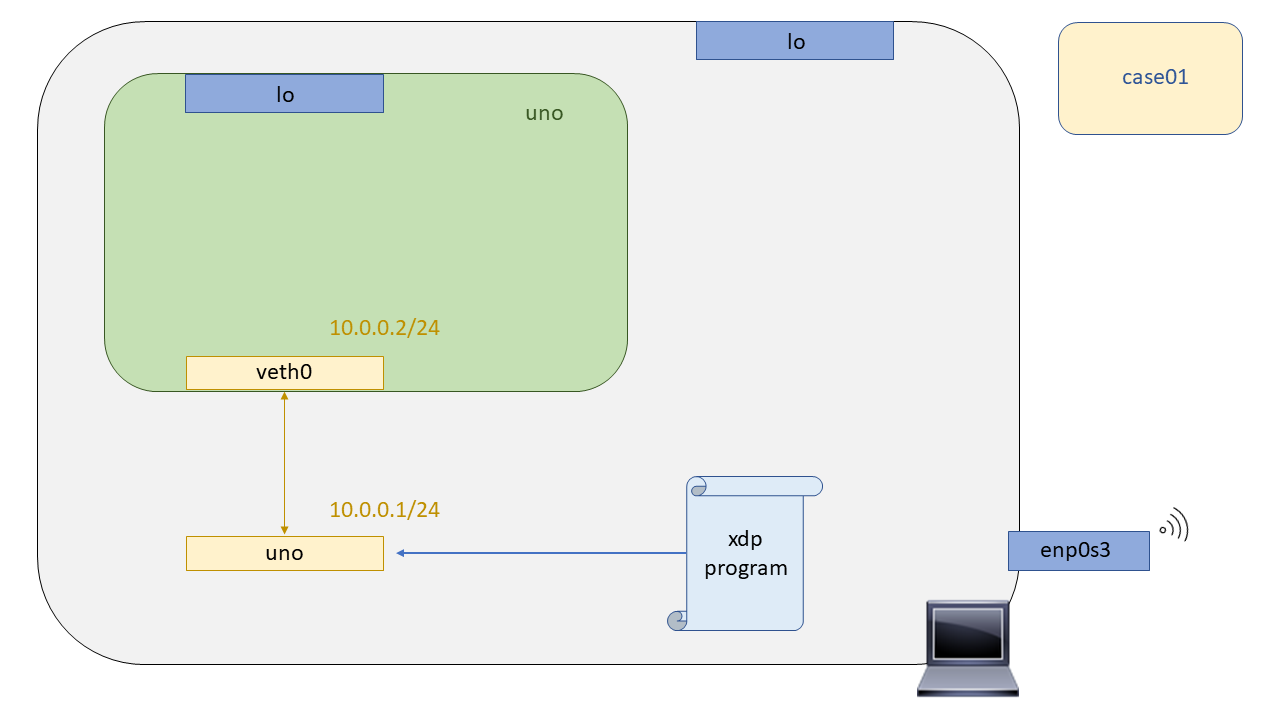
\includegraphics[width=16cm]{archivos/img/dev/xdp/case01/scenario.png}
    \caption{Escenario cableado del Case01 - XDP}
    \label{fig:case01_xdp_ether_scenario}
\end{figure}

\vspace{0.9cm}
\textbf{Carga del programa XDP}\\
\par

Es hora de cargar el programa \gls{xdp} en el Kernel. Para realizarlo, habría
dos maneras de cargar el bytecode en el Kernel. La primera sería hacer uso de la herramienta iproute2 (\ref{iproute2}) a partir de la versión \texttt{v4.12}. La segunda, y la más utilizada debido a las limitaciones de iproute2 para trabajar con los mapas \gls{bpf}, es hacer uso de la librería \textbf{libbpf}\footnote{\url{https://github.com/libbpf/libbpf}}. En este caso se hará uso de un programa hecho en C haciendo uso de dicha librería para cargar los programas \gls{xdp} en el kernel, mapas \gls{bpf} y demás. El código de dicho programa se puede encontrar \href{https://github.com/davidcawork/TFG/blob/master/src/use_cases/xdp/util/xdp_loader.c}{\textbf{aquí}}. Este \textit{loader} fue desarrollado siguiendo el tutorial de los desarrolladores del kernel de Linux llamado xdp-tutorial\footnote{\url{https://github.com/xdp-project/xdp-tutorial}}. \\
\par
Al \textit{loader} se le está indicando \texttt{-d} (\textit{device}), \texttt{-F} (\textit{Force}) para que haga un \textit{override} en caso de que ya haya un programa \gls{xdp} anclado a dicha interfaz, y por último, se le indica el \texttt{--progsec} (\textit{program section}) utilizados en \gls{xdp} para englobar distintas funcionalidades en un mismo \textit{bytecode} compilado. 

\begin{lstlisting}[language= bash, style=Consola, caption={Carga del programa XDP - Case01},label=code:case01_xdp_ether_load]
    # Cargaremos el programa sobre la interfaz "uno" 
    sudo ./xdp_loader -d uno -F --progsec xdp_case01
\end{lstlisting}

\vspace{1cm}
\textbf{Comprobación del funcionamiento}\\
\par

Una vez que el programa \gls{xdp} fue anclado a la interfaz se comprobará de que funciona según lo esperado. Esto se hará generando tráfico desde un extremo de una \gls{veth} para que atraviese por la interfaz que tiene anclado el programa \gls{xdp}. En este caso el comportamiento esperado del programa \gls{xdp} es que haga un drop de los paquetes nada más llegar a la interfaz \texttt{uno}.

% figura escenario
\begin{figure}[ht]
    \centering
    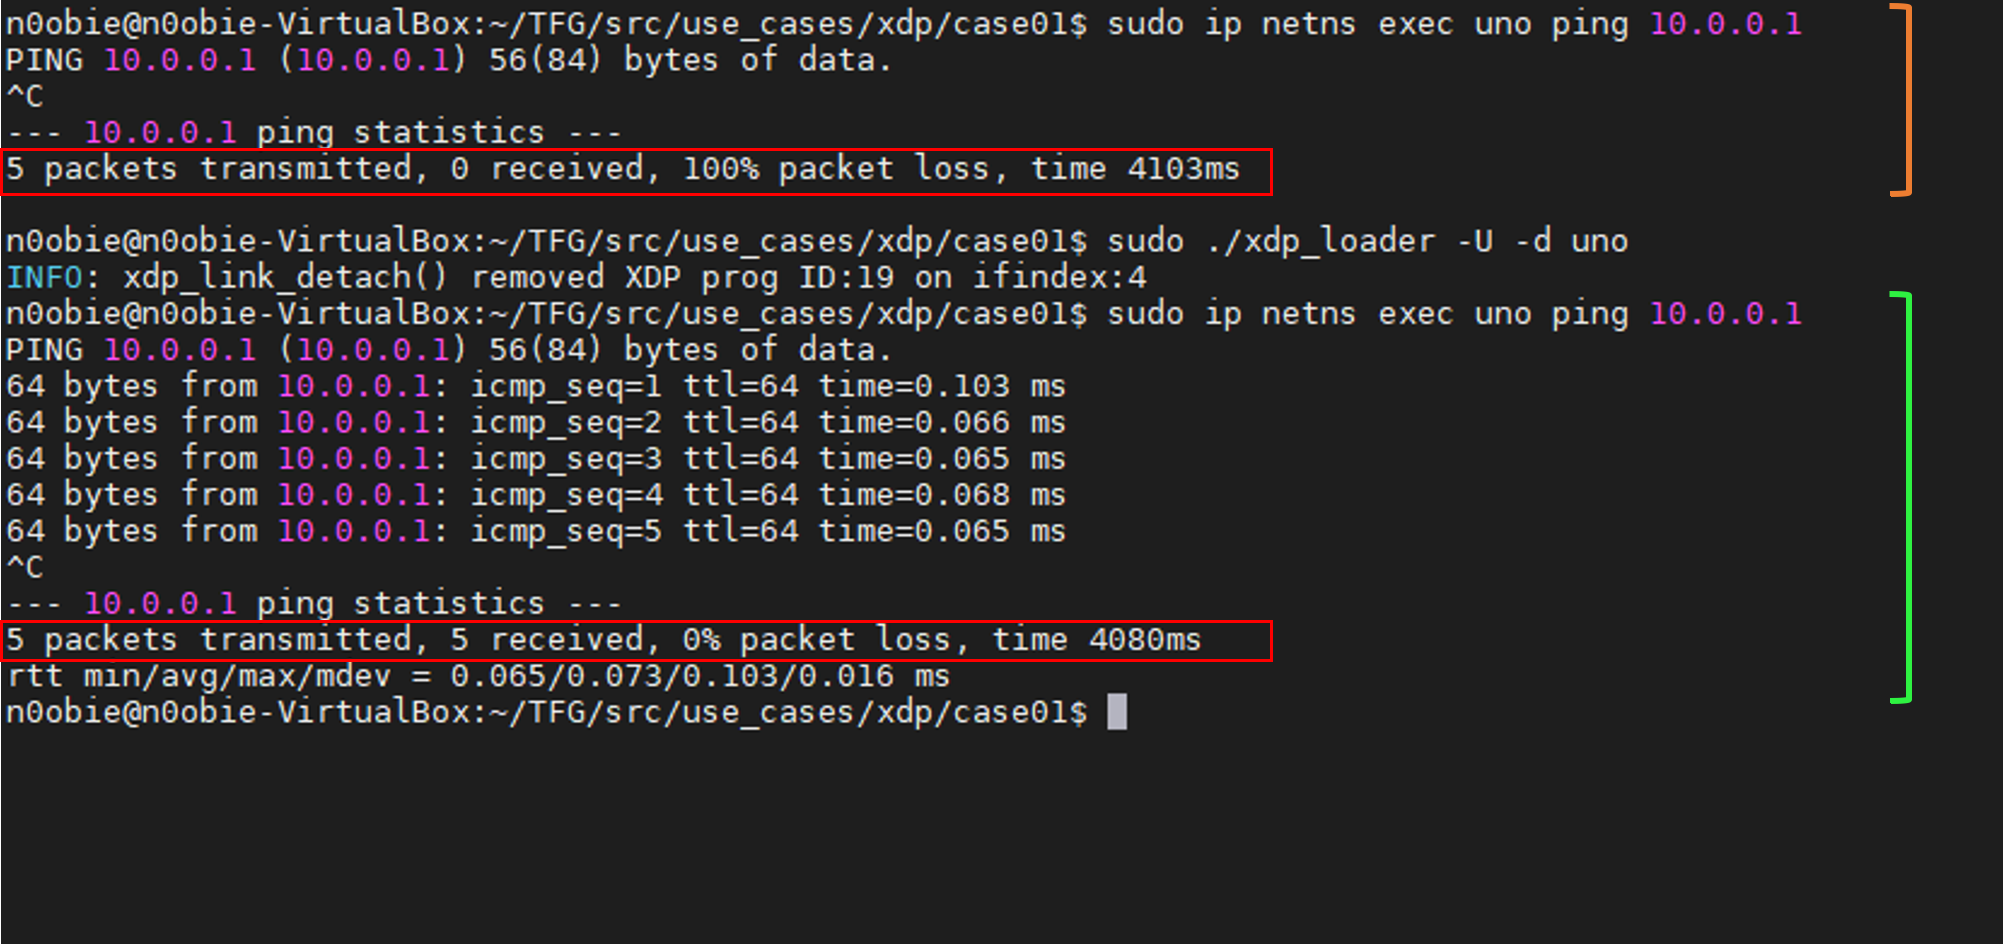
\includegraphics[width=15.5cm]{archivos/img/dev/xdp/case01/demo_case01_edited.png}
    \caption{Comprobación de funcionamiento del Case01 - XDP}
    \label{fig:case01_xdp_ether_func}
\end{figure}

Como se puede ver en la figura \ref{fig:case01_xdp_ether_func}, se accede al interior de la \textit{Network namespace} \texttt{uno} y se realiza un ping \fcolorbox{black}{orange}{\rule{0pt}{2.5pt}\rule{2.5pt}{0pt}}\hspace{1mm}  hacia la interfaz con el programa XDP. Se puede apreciar que no hay conectividad, por lo que el programa \gls{xdp} desarrollado está funcionando según lo esperado. Para corroborar que la falta de conectividad se debe al programa \gls{xdp}, se va a desanclar de la interfaz y se probará de nuevo la conectividad. Según se puede ver en el último ping \fcolorbox{black}{green}{\rule{0pt}{2.5pt}\rule{2.5pt}{0pt}} , ya hay conectividad, por lo que se afirma que realmente los paquetes que atravesaban la interfaz eran descartados por el programa \gls{xdp}. \newpage





\subsection{Case02 - Pass}
\label{xdp_ether_case02}

En este caso de uso se probará que es posible admitir todos los paquetes recibidos en la interfaz donde está anclado el programa \gls{xdp}. Pero podría surgir la siguiente pregunta: ¿qué significa ``Admitir”? Se quiere comprobar si es posible dejar pasar los paquetes, sin que les afecte el datapath programado con la tecnología. El motivo es que, aunque \gls{xdp} se concibe normalmente como como un mecanismo para hacer un \textit{by-pass} al \textit{stack} de red del Kernel de Linux (es decir, una completa redefinición del mismo), en muchas ocasiones será útil trabajar en conjunto para conseguir la funcionalidad deseada. \\
\par
Para la realizar la prueba, al igual que en el case01 (\ref{xdp_ether_case01}) primero se deberá compilar el programa \gls{xdp}, acto seguido levantar el escenario donde se va a realizar la prueba, y por último, anclar el binario a una interfaz del escenario.

\begin{lstlisting}[language=C, style=C-color, caption={Programa básico XDP - Case01},label=code:case02_xdp_ether_kernprog]
    SEC("xdp_case02")
    int xdp_pass_func(struct xdp_md *ctx)
    {
    	int action = XDP_PASS;
    	goto out;
    out:
            return xdp_stats_record_action(ctx, action);
    }
    
    char _license[ ] SEC("license") = "GPL";
\end{lstlisting}
\vspace{0.5cm}

Como se puede ver en el bloque \ref{code:case02_xdp_ether_kernprog}, el programa es exactamente igual al desarrollado en el case01 (\ref{xdp_ether_case01}) cambiando únicamente el código de retorno \gls{xdp}. De esta forma se consigue modificar la funcionalidad del programa, a la deseada.\\

\vspace{0.3cm}
\textbf{Compilación}\\
\par

Para compilar el programa \gls{xdp} se ha dejado un Makefile preparado en este directorio al igual que en el case01 (\ref{xdp_ether_case01}), por lo que para compilarlo únicamente hay que seguir las indicaciones del bloque \ref{code:case02_xdp_ether_compilacion}.

\begin{lstlisting}[language= bash, style=Consola, caption={Compilación programa XDP - Case02},label=code:case02_xdp_ether_compilacion]
    # En caso de no haber entrado en el directorio asignado del caso de uso
    cd TFG/src/use_cases/xdp/case02
    
    
    # Hacemos uso del Makefile suministrado 
    sudo make
\end{lstlisting}
\vspace{0.5cm}

Ahora bien, en el anterior caso de uso no se quiso incidir demasiado en este aspecto, pero ¿Cómo se produce la compilación de los programas \gls{xdp}?  Como ya se ha podido ver, los programas \gls{xdp} están escritos en lo que llaman un lenguaje C restringido, en los cuales la secuencia de programa siempre empieza por ``xdp". Esto es así ya que, si no, el verificador del Kernel no podrá saber de que tipo de \textit{bytecode} se trata y lo rechazará.\\
\par

Este código C restringido, se compilará haciendo uso de la herramienta \textbf{clang} cómo compilador de \textit{frontend}, y de la herramienta \textbf{LLVM} cómo compilador de  \textit{backend}. De esta manera se generará un \textit{bytecode} \gls{bpf}, y posteriormente se almacenará en un objeto de tipo \gls{elf}. Estos últimos serán los que se carguen en el Kernel (\texttt{*.o}). Es curioso el hecho de entender cómo pasamos de los hipotéticos programas \gls{xdp} (C restringido) a \textit{bytecode} \gls{bpf}, ya que, cuando se indaga un poco más en \gls{xdp}, se llega a la conclusión de que \gls{xdp} se podría ver como un \textit{framework} de \gls{bpf} para trabajar a nivel de \gls{nic}.\\
\par
Hay más factores que lo diferencian de los programas \gls{bpf}, como son las estructuras de datos que manejan, además de los metadatos; pero al fin y al cabo, para anclar un programa \gls{xdp} este debe antes ser traducido a un \textit{bytecode} \gls{bpf}.\\

\vspace{0.7cm}
\textbf{Puesta en marcha del escenario}\\
\par

Para testear los programas \gls{xdp} se hará uso de las \textit{Network Namespaces} (más información en la sección \ref{namespaces}). Como ya se comentaba, para que no suponga una barrera de entrada el concepto de las \textit{Network Namespaces}, se ha dejado escrito un script para levantar el escenario, y para su posterior limpieza. Es importante señalar que el script debe ser lanzado con permisos de root. Para levantar el escenario se debe ejecutar dicho script como se indica en el bloque \ref{code:case02_xdp_ether_escenario}.\\
\par
Para limpiar la máquina del escenario recreado anteriormente, se puede correr el mismo script indicándole ahora el parámetro \texttt{-c} (\textit{Clean}). En el peor de los casos, y si se cree que la limpieza se no se ha realizado de manera satisfactoria, se puede llevar a cabo un reinicio de la máquina consiguiendo así que todos los entes no persistentes (\gls{veth}, netns..) desaparezcan del equipo.

\begin{lstlisting}[language= bash, style=Consola, caption={Puesta en marcha del escenario - Case02},label=code:case02_xdp_ether_escenario]
    # Para levantar el escenario (Importante hacerlo con permisos de super usuario)
    sudo ./runenv.sh -i
    
    
    # Una vez finalizado la comprobación del caso de uso, limpiaremos nuestra maquina:
    sudo ./runenv.sh -c
\end{lstlisting}
\vspace{0.5cm}

El escenario que se va a manejar en este caso de uso es el siguiente (Ver figura \ref{fig:case02_xdp_ether_scenario}), compuesto únicamente de una \textit{Network Namespace} (\texttt{uno}) y un par de \gls{veth}s (\texttt{veth0} -- \texttt{uno}) para comunicar la \textit{Network Namespace} creada con la \textit{Network Namespace} por defecto.

\newpage

% figura escenario
\begin{figure}[ht]
    \centering
    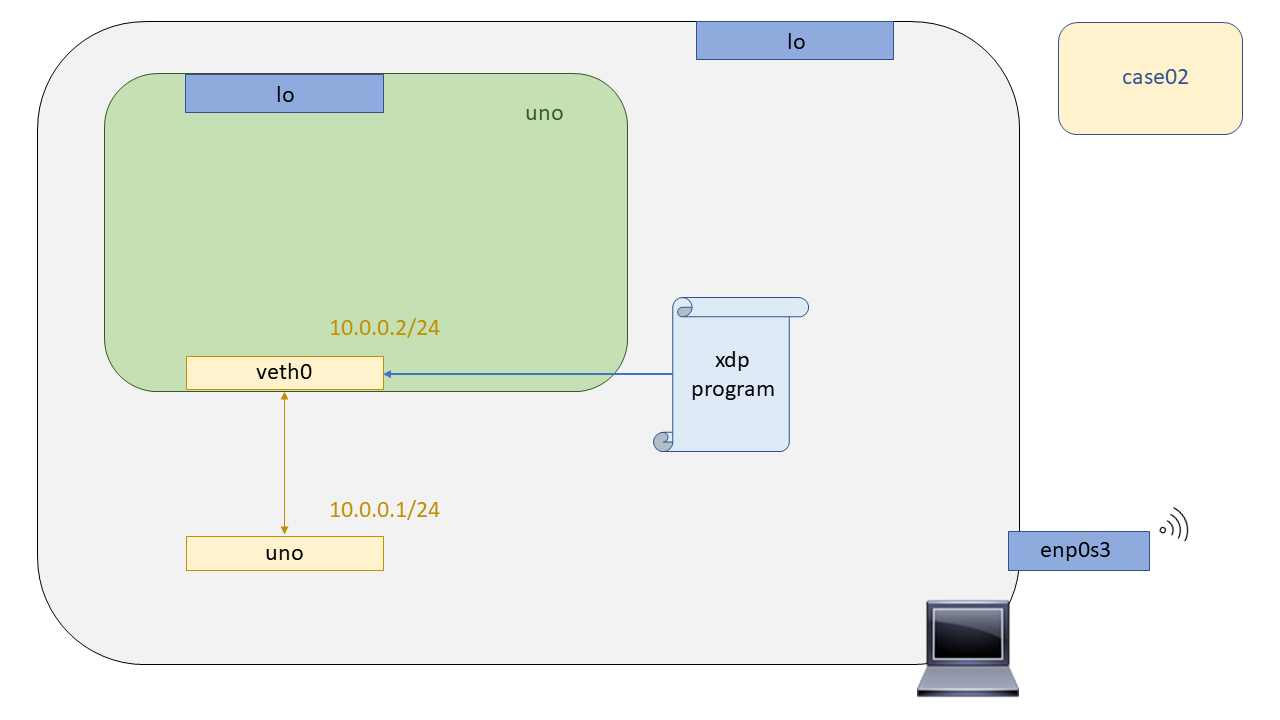
\includegraphics[width=16cm]{archivos/img/dev/xdp/case02/scenario.png}
    \caption{Escenario cableado del Case02 - XDP}
    \label{fig:case02_xdp_ether_scenario}
\end{figure}

\vspace{0.5cm}
\textbf{Carga del programa \gls{xdp}}\\
\par
Una vez que se tiene el escenario y el programa \gls{xdp} compilado, se procederá a cargarlo en el Kernel. Para más información sobre el programa  xdp\_loader, qué aporta la librería libbpf, o por que no se hace uso de la herramienta iproute2 para cargar los programas \gls{xdp} en el Kernel, se recomienda regresar al case01 (\ref{xdp_ether_case01})  donde se intenta abordar todas estas cuestiones.\\
\par

Como se comentaba, es hora de cargar el programa en el Kernel, esta vez por variar se va a cargar el programa \gls{xdp} en el extremo de la \gls{veth} que se encuentra en el interior de la \textit{Network Namespace}. Se podría haber hecho de la misma manera que en el caso de uso anterior y cargar el programa \gls{xdp} en la \gls{veth} que se ve desde la \textit{Network Namespace} por defecto, pero de esta manera se explorará como ejecutar comandos ``dentro" de una \textit{Network Namespace}. Para ejecutar comandos ``dentro" de una \textit{Network Namespace} se hará uso de la herramienta iproute2 (\ref{iproute2}), más concretamente su módulo llamado \textbf{netns}. A la herramienta se le debe indicar el parámetro \texttt{exec} y el nombre de la \textit{Network Namespace} dónde se quiera ejecutar el comando, y por último, se le indicará el comando que correrá ``dentro" de la \textit{Network Namespace}.

\begin{lstlisting}[language= bash, style=Consola, caption={Carga del programa XDP - Case02},label=code:case02_xdp_ether_load]
    # Cargaremos el programa sobre la interfaz "veth0" 
    sudo ip netns exec uno ./xdp_loader -d veth0 -F --progsec xdp_case02
\end{lstlisting}
\vspace{0.2cm}

Por lo que, entendiendo como funciona el módulo netns, y los parámetros suministrados al programa xdp\_loader, explicados en el caso de uso case01 (\ref{xdp_ether_case01}), se podrá intuir que el resultado de la sentencia anterior es la de cargar el programa \gls{xdp} en la interfaz llamada \texttt{veth0} contenida en la \textit{Network Namespace} \texttt{uno}.


\vspace{1.2cm}
\textbf{Comprobación del funcionamiento}\\
\par


La comprobación del funcionamiento del programa \gls{xdp} anclado a la interfaz \texttt{veth0} se llevará a cabo testeando la conectividad entre el par de \gls{veth}s. Puede que sea una prueba un poco simple, pero es suficiente, ya que únicamente se quiere verificar que el programa anclado en la interfaz está delegando los paquetes que le llegan, al \textit{stack} de red.\\
\par

En este punto se quiere comentar un aspecto de \gls{xdp}, y es que, desde que se empezó a trabajar con \gls{xdp}, se veía al \textit{stack} de red de Linux como a un enemigo a batir, o ``by-passear"; ya que con \gls{xdp} se quiere conseguir definir de manera exclusiva el datapath que se desea implementar con un equipo que porte el Kernel de Linux.  De esta manera, se consigue técnicamente un rendimiento superior ya que se quita de encima toda la redundancia y capas que no son necesarias para el procesamiento del hipotético datapath.\\
\par
Ahora bien, en el transcurso del aprendizaje con esta tecnología se ha visto que en ocasiones trabajar de manera cooperativa con el \textit{stack} de red puede reportar muchas facilidades y muchas otras funcionalidades ya implementadas en éste. No es cuestión de reinventar la rueda, más que nada porque el rendimiento que se puede llegar a ganar por hacer todo el procesamiento de manera exclusiva en la propia \gls{nic}, en opinión del autor, no compensa con la robustez y fiabilidad que tendrá dicha funcionalidad en el \textit{stack} de red de Linux.\\
\par
Como se puede apreciar en la figura \ref{fig:case02_xdp_ether_func}, prestando atención al ping \fcolorbox{black}{green}{\rule{0pt}{2.5pt}\rule{2.5pt}{0pt}}  (Fig. \ref{fig:case02_xdp_ether_func_ping}), hay perfecta conectividad. Eso significa que el programa \gls{xdp} está delegando correctamente los paquetes al \textit{stack} de red, se puede verificar dicho funcionamiento atendiendo a las estadísticas sobre los códigos de retorno de la figura \ref{fig:case02_xdp_ether_func_stats}, dónde el código de retorno \texttt{XDP\_PASS} va en aumento. Dichas estadísticas han sido recolectadas haciendo uso del binario xdp\_stats. En el siguiente caso de uso se explicará brevemente el funcionamiento de la recolección de estadísticas de los programas \gls{xdp}. 
\newpage

\begin{figure}[h!]
    \centering
    \begin{subfigure}[b]{\textwidth}
    	\centering
        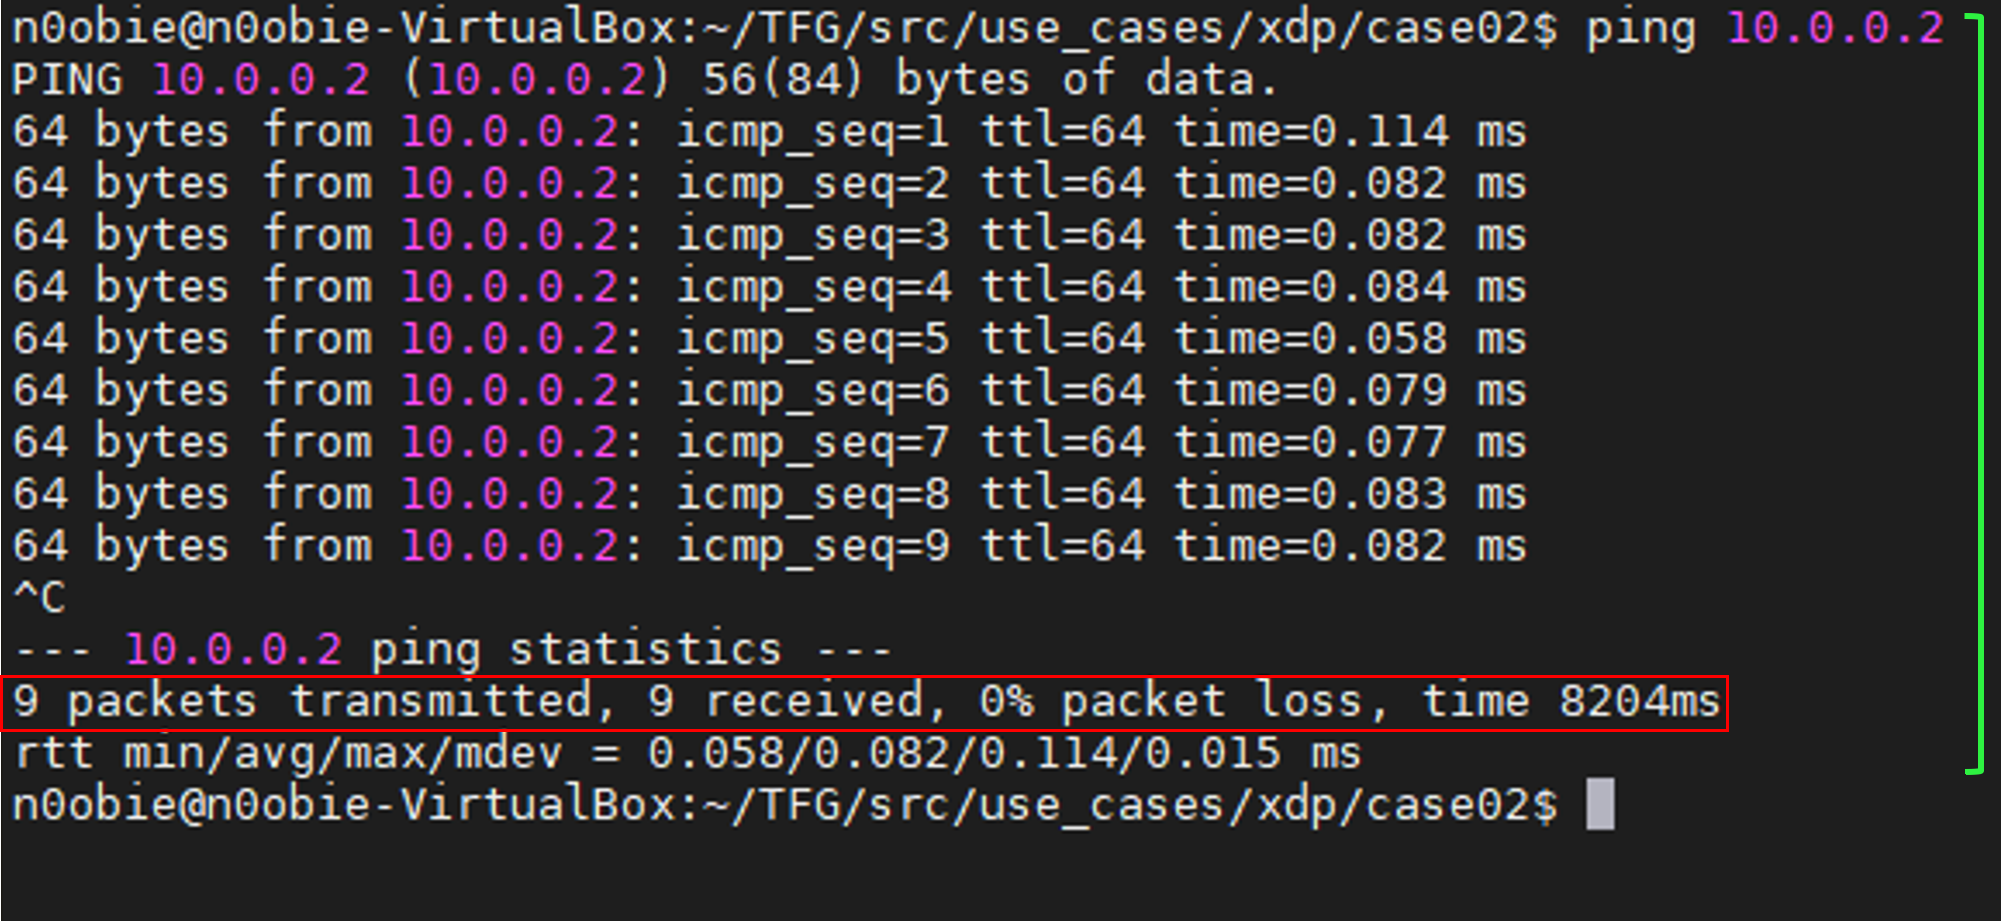
\includegraphics[width=11cm]{archivos/img/dev/xdp/case02/demo_case02_3_edited.png}
        \caption{Ejecución de ping hacia la interfaz con el programa XDP}
        \label{fig:case02_xdp_ether_func_ping}
    \end{subfigure}
    \par\bigskip
    \begin{subfigure}[b]{\textwidth}
    	\centering
    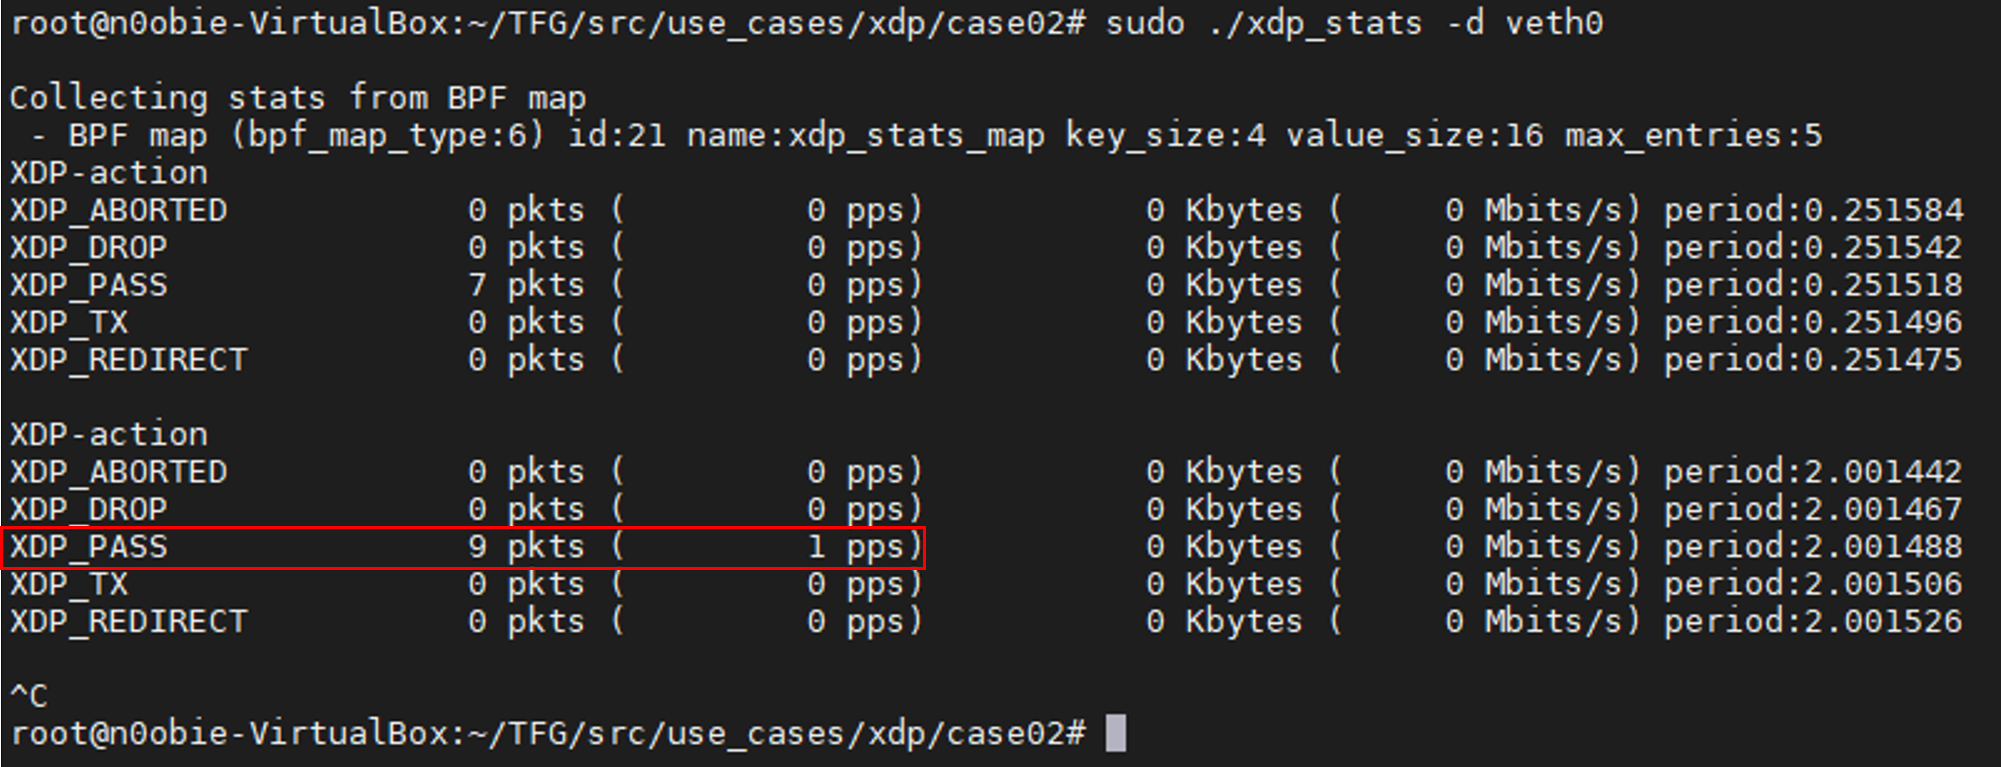
\includegraphics[width=14cm]{archivos/img/dev/xdp/case02/demo_case02_4_edited.png}
        \caption{Estadísticas de los códigos de retorno XDP}
        \label{fig:case02_xdp_ether_func_stats}
    \end{subfigure}
    \caption{Comprobación de funcionamiento del Case02 - XDP}
    \label{fig:case02_xdp_ether_func}
\end{figure}


\vspace{0.3cm}
\subsection{Case03 - Echo server}
\label{xdp_ether_case03}


En este caso de uso se hará un especial hincapié en el análisis de paquetes, su filtrado y manejo. En los anteriores caso de uso se definía un comportamiento de los paquetes haciendo un uso exclusivo de los códigos de retorno \gls{xdp}, más concretamente \texttt{XDP\_DROP} para tirar los paquetes y \texttt{XDP\_PASS} para admitir los paquetes. Hay más códigos de retorno \gls{xdp} pero con ellos no se puede lograr desarrollar todas las lógicas posibles. Como ya se comentaba en la sección \ref{TecnologiaXDP}, estos códigos se encuentran definidos en el archivo de cabecera \texttt{bpf.h}. En la tabla \ref{tab:xdp_return_code} se pueden recordar y ver qué funcionalidad aportaba cada uno de ellos.\\
\par
\vspace{0.3cm}

\begin{table}[ht]
\centering
\resizebox{\textwidth}{!}{%
\begin{tabular}{|c|c|}
\hline
\rowcolor[HTML]{EFEFEF} 
\multicolumn{1}{|l|}{\cellcolor[HTML]{EFEFEF}{\color[HTML]{24292E} \textbf{Código de Retorno}}} & \textbf{Comportamiento}                                                              \\ \hline
\texttt{XDP\_PASS}                                                                                       & Admitir el paquete, pasarselo al \textit{stack} de red                                        \\ \hline
\texttt{XDP\_DROP}                                                                                       & Tirar el paquete                                                                     \\ \hline
\texttt{XDP\_ABORTED}                                                                                    & Tirar el paquete y generar una \texttt{xdp:xdp\_exception}, útiles para depurar               \\ \hline
\texttt{XDP\_REDIRECT}                                                                                   & Utilizado cuando se realiza un forwarding del paquete a otra interfaz                \\ \hline
\texttt{XDP\_TX}                                                                                         & Re-transmitir el paquete por la misma interfaz por la cual se ha recibido el paquete \\ \hline
\end{tabular}}
\caption{Resumen sobre los códigos de retorno XDP}
\label{tab:xdp_return_code}
\end{table}


Ahora bien, ¿Cómo se puede implementar una lógica más avanzada? Esto se podrá conseguir filtrando los paquetes, y en base al tipo de paquete aplicar unas acciones u otras haciendo uso de los códigos de retorno \gls{xdp}. Para filtrar paquetes, se tendrá que hacer uso de las estructuras de datos de los protocolos de red definidas en el Kernel de Linux. Además de hacer numerosas comprobaciones de limites de acceso a memoria, para que el verificador del Kernel no nos tire el paquete por un acceso indebido según se comentaba en las limitaciones \gls{xdp} (Sección \ref{TecnologiaXDP}). Las estructuras de datos que han sido utilizadas para filtrar paquetes en este caso de uso se dejan indicadas en la tabla \ref{tab:xdp_structs}.\\
\par


\begin{table}[ht]
\centering

\begin{tabular}{|c|c|}
\hline
\rowcolor[HTML]{EFEFEF} 
\multicolumn{1}{|l|}{\cellcolor[HTML]{EFEFEF}{\color[HTML]{24292E} \textbf{Estructura}}} & \multicolumn{1}{l|}{\cellcolor[HTML]{EFEFEF}{\color[HTML]{24292E} \textbf{Archivo de cabecera}}} \\ \hline
\texttt{struct ethhdr}                                                                            & \texttt{<linux/if\_ether.h>}                                                                               \\ \hline
\texttt{struct ipv6hdr}                                                                           & \texttt{<linux/ipv6.h>}                                                                                   \\ \hline
\texttt{struct iphdr}                                                                             & \texttt{<linux/ip.h>}                                                                                     \\ \hline
\texttt{struct icmp6hdr}                                                                          & \texttt{<linux/icmpv6.h>}                                                                                 \\ \hline
\texttt{struct icmphdr}                                                                           & \texttt{<linux/icmp.h>}                                                                                   \\ \hline
\end{tabular}
\caption{Estructuras de datos para procesar las cabeceras de los paquetes}
\label{tab:xdp_structs}
\end{table}


Es importante señalar que los paquetes vienen por la red en un \textit{byte order} denominado como  \textit{Network byte order}. Por esta razón, se necesitará traducirlo al \textit{byte order} usado por la máquina ( \textit{Host order} ) en el caso de que se quiera comprobar o hacer uso del valor de algunos de sus campos. Para ello, se hará uso de las funciones \texttt{bpf\_ntohs()} y \texttt{bpf\_htons()} respectivamente.\\
\par

Por lo tanto, sabiendo qué estructuras de datos utilizar para el filtrando los paquetes, se filtrarán todos los paquetes de tipo ICMP - ICMPv6 con un código \texttt{ICMP-ECHO}. El resto de paquetes se le delegarán al \textit{stack} de red para que los maneje. En cuanto a los paquetes ICMP filtrados, se contestarán  automáticamente desde el programa \gls{xdp} desarrollado. Esto se conseguirá en la propia \gls{nic}, cambiando el \texttt{ICMP-ECHO} por un \texttt{ICMP-REPLY}, cambiando MACs, y por último, actualizando el \textit{checksum} de la cabecera ICMP. Como en este caso el paquete debe ser reenviado por la misma interfaz por la cual se recibió, se hará uso de código de retorno \texttt{XDP\_TX}.

\vspace{1cm}
\textbf{Compilación}\\
\par

Para compilar el programa \gls{xdp} se ha dejado un Makefile preparado en este directorio al igual que en el case02 (\ref{xdp_ether_case02}), por lo que para compilarlo únicamente hay que seguir las indicaciones del bloque \ref{code:case03_xdp_ether_compilacion}.

\begin{lstlisting}[language= bash, style=Consola, caption={Compilación programa XDP - Case03},label=code:case03_xdp_ether_compilacion]
    # En caso de no haber entrado en el directorio asignado del caso de uso
    cd TFG/src/use_cases/xdp/case03
    
    
    # Hacemos uso del Makefile suministrado 
    sudo make
\end{lstlisting}
\vspace{0.5cm}

Para más información sobre el proceso de compilación del programa \gls{xdp}, recomendamos que vuelva al case02 (\ref{xdp_ether_case02}) donde se hace referencia al flujo dispuesto para la compilación de los programas \gls{xdp}.


\vspace{0.7cm}
\textbf{Puesta en marcha del escenario}\\
\par
Para comprobar el funcionamiento de los programas \gls{xdp} se hará uso de nuevo de las \textit{Network Namespace} (más información en la sección \ref{namespaces}). Como ya se comentaba, para que no suponga una barrera de entrada el concepto de las \textit{Network Namespace}, se ha dejado escrito un script para levantar el escenario, y para su posterior limpieza. Es importante señalar que el script debe ser lanzado con permisos de root. Para levantar el escenario debemos ejecutar dicho script como se indica en el bloque \ref{code:case03_xdp_ether_escenario}. Para limpiar la máquina del escenario recreado anteriormente, se puede correr el mismo script indicándole ahora el parámetro \texttt{-c} (\textit{Clean}). En el peor de los casos, y si se cree que la limpieza se no se ha realizado de manera satisfactoria, se puede llevar a cabo un reinicio de la máquina consiguiendo así que todos los entes no persistentes (\gls{veth}, netns..) desaparezcan del equipo.

\begin{lstlisting}[language= bash, style=Consola, caption={Puesta en marcha del escenario - Case03},label=code:case03_xdp_ether_escenario]
    # Para levantar el escenario (Importante hacerlo con permisos de super usuario)
    sudo ./runenv.sh -i
    
    
    # Una vez finalizado la comprobación del caso de uso, limpiaremos nuestra máquina:
    sudo ./runenv.sh -c
\end{lstlisting}
\vspace{0.5cm}

El escenario que se va a manejar en este caso de uso es el siguiente (Ver figura \ref{fig:case03_xdp_ether_scenario}), compuesto únicamente de una \textit{Network Namespace} (\texttt{uno}) y un par de \gls{veth}s (\texttt{veth0} -- \texttt{uno}) para comunicar la \textit{Network Namespace} creada con la \textit{Network Namespace} por defecto.

% figura escenario
\begin{figure}[ht]
    \centering
    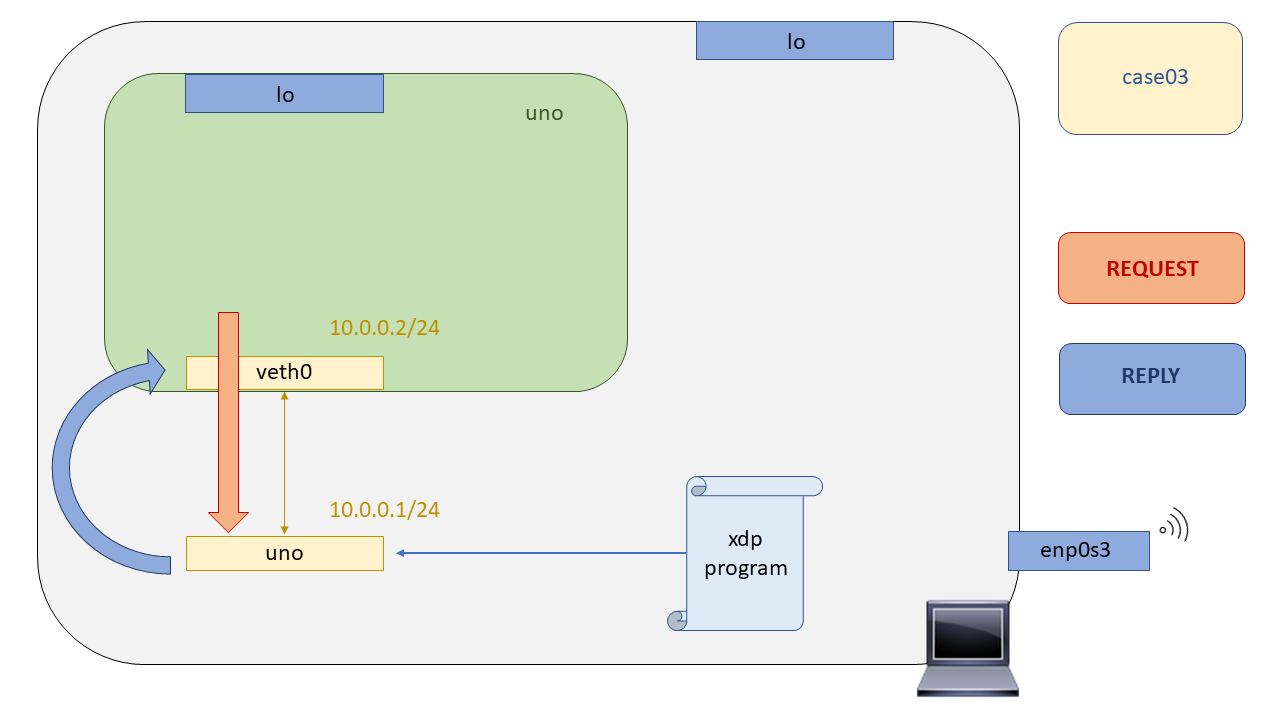
\includegraphics[width=16cm]{archivos/img/dev/xdp/case03/scenario.png}
    \caption{Escenario cableado del Case03 - XDP}
    \label{fig:case03_xdp_ether_scenario}
\end{figure}


\vspace{0.7cm}
\textbf{Carga del programa XDP}\\
\par
Una vez que se tiene el escenario levantado y el programa \gls{xdp} compilado, se procederá a cargarlo en el Kernel. Para más información sobre el programa xdp\_loader, qué aporta la librería libbpf, o por que no se hace uso de la herramienta iproute2 para cargar los programas \gls{xdp} en el Kernel,  se recomienda regresar al case01 (\ref{xdp_ether_case01})  donde se intenta abordar todas estas cuestiones. De forma adicional, es interesante comentar que se va hacer uso del módulo \textbf{netns} de la herramienta iproute2, si tiene alguna duda sobre dicho módulo le recomendamos que consulte su \textit{man-page} o vuelva al case02 (\ref{xdp_ether_case02}) donde se hace una pequeña introducción sobre éste, y su funcionamiento básico para ejecutar comandos ``dentro" de una \textit{Network Namespace}.

\begin{lstlisting}[language= bash, style=Consola, caption={Carga del programa XDP - Case03},label=code:case03_xdp_ether_load]
    # Anclamos el programa XDP (xdp_pass) en la interfaz veth0, perteneciente a la Network Namespace "uno" 
    sudo ip netns exec uno ./xdp_loader -d veth0 -F --progsec xdp_pass
    
    # Anclamos el programa XDP en la interfaz uno, perteneciente a la Network Namespace por defecto
    sudo ./xdp_loader -d uno -F --progsec xdp_case03
\end{lstlisting}
\vspace{0.5cm}

En este caso de uso se anclará el programa \gls{xdp} a validar en la \gls{veth} exterior, por lo que las pruebas vendrán inducidas desde ``dentro" de la \textit{Network Namespace} \texttt{uno}. Para anclar el programa se ha hecho uso de nuevo del programa xdp\_loader. Es importante señalar que se ha tenido que anclar un \textit{dummy program} que permite pasar todos los paquetes a la \gls{veth} destino, esta es una limitación propia por trabajar con \gls{veth}s y \gls{xdp}, de momento se trata de una limitación de implementación, pero puede que a un corto plazo esta limitación se vea ya superada. \\
\par
Para más información sobre esta limitación recomendamos ver la charla de la Netdev llamada ``\textit{\gls{veth}: \gls{xdp} for containers}"\footnote{\url{https://netdevconf.info/0x13/session.html?talk-veth-xdp}} donde explican con un mayor detalle la misma, cómo abordarla y por qué está inducida.

\vspace{0.5cm}
\textbf{Comprobación del funcionamiento}\\
\par

La comprobación del funcionamiento del programa \gls{xdp} anclado a la interfaz \texttt{uno} se llevará a cabo generando pings desde ``dentro" la \textit{Network Namespace} \texttt{uno} hacia afuera. De esta forma la interfaz \texttt{uno} los filtrará, analizará y generará una respuesta. \\
\par
El funcionamiento del programa xdp\_stats es muy simple, ya que desde el programa anclado en el Kernel se genera un mapa \gls{bpf} del tipo clave-valor, donde las claves son los distintos códigos de retorno y los valores son contadores. Después, desde el espacio de usuario el programa xdp\_stats, sabiendo el nombre del mapa \gls{bpf}, y dónde se almacena, va a buscarlo. Para ello, abre el descriptor de archivo asociado a ese mapa almacenado en el path \texttt{/sys/fs/bpf/}. Una vez que tiene abierto el descriptor de archivo, este irá leyendo por clave del mapa todas las estadísticas sobre los códigos de retorno de forma periódica.


\begin{figure}[ht]
    \centering
    \begin{subfigure}[b]{\textwidth}
    	\centering
        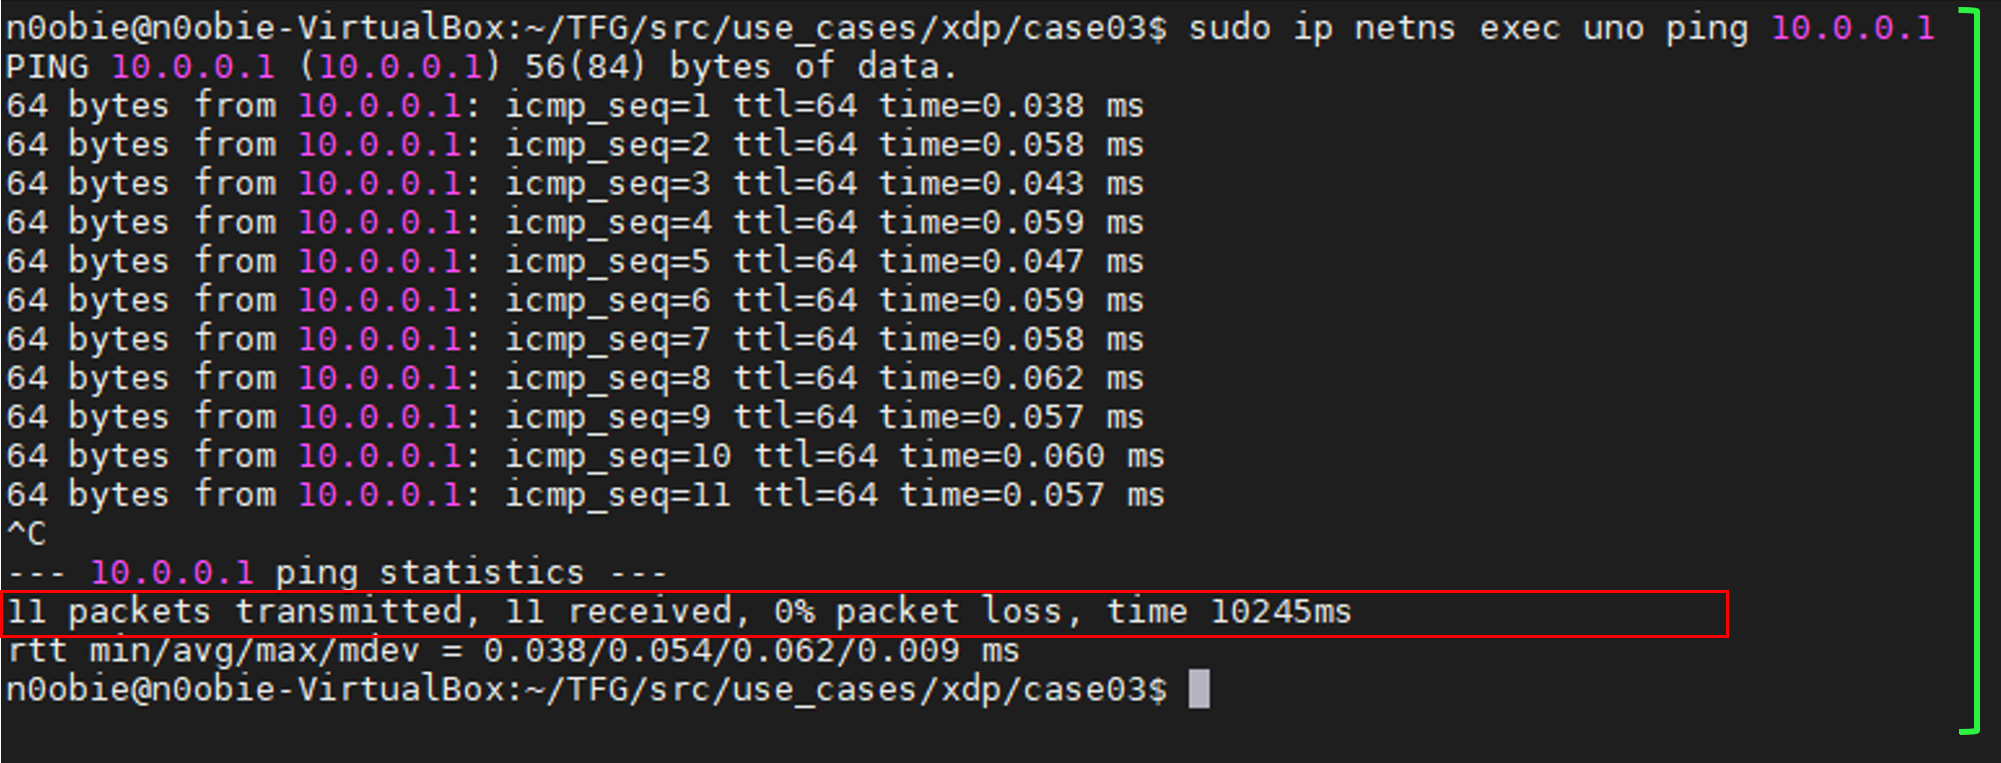
\includegraphics[width=12cm]{archivos/img/dev/xdp/case03/demo_case03_2_edited.png}
        \caption{Ejecución de ping hacia la interfaz con el programa XDP}
        \label{fig:case03_xdp_ether_func_ping}
    \end{subfigure}
    \par\bigskip
    \begin{subfigure}[b]{\textwidth}
    	\centering
        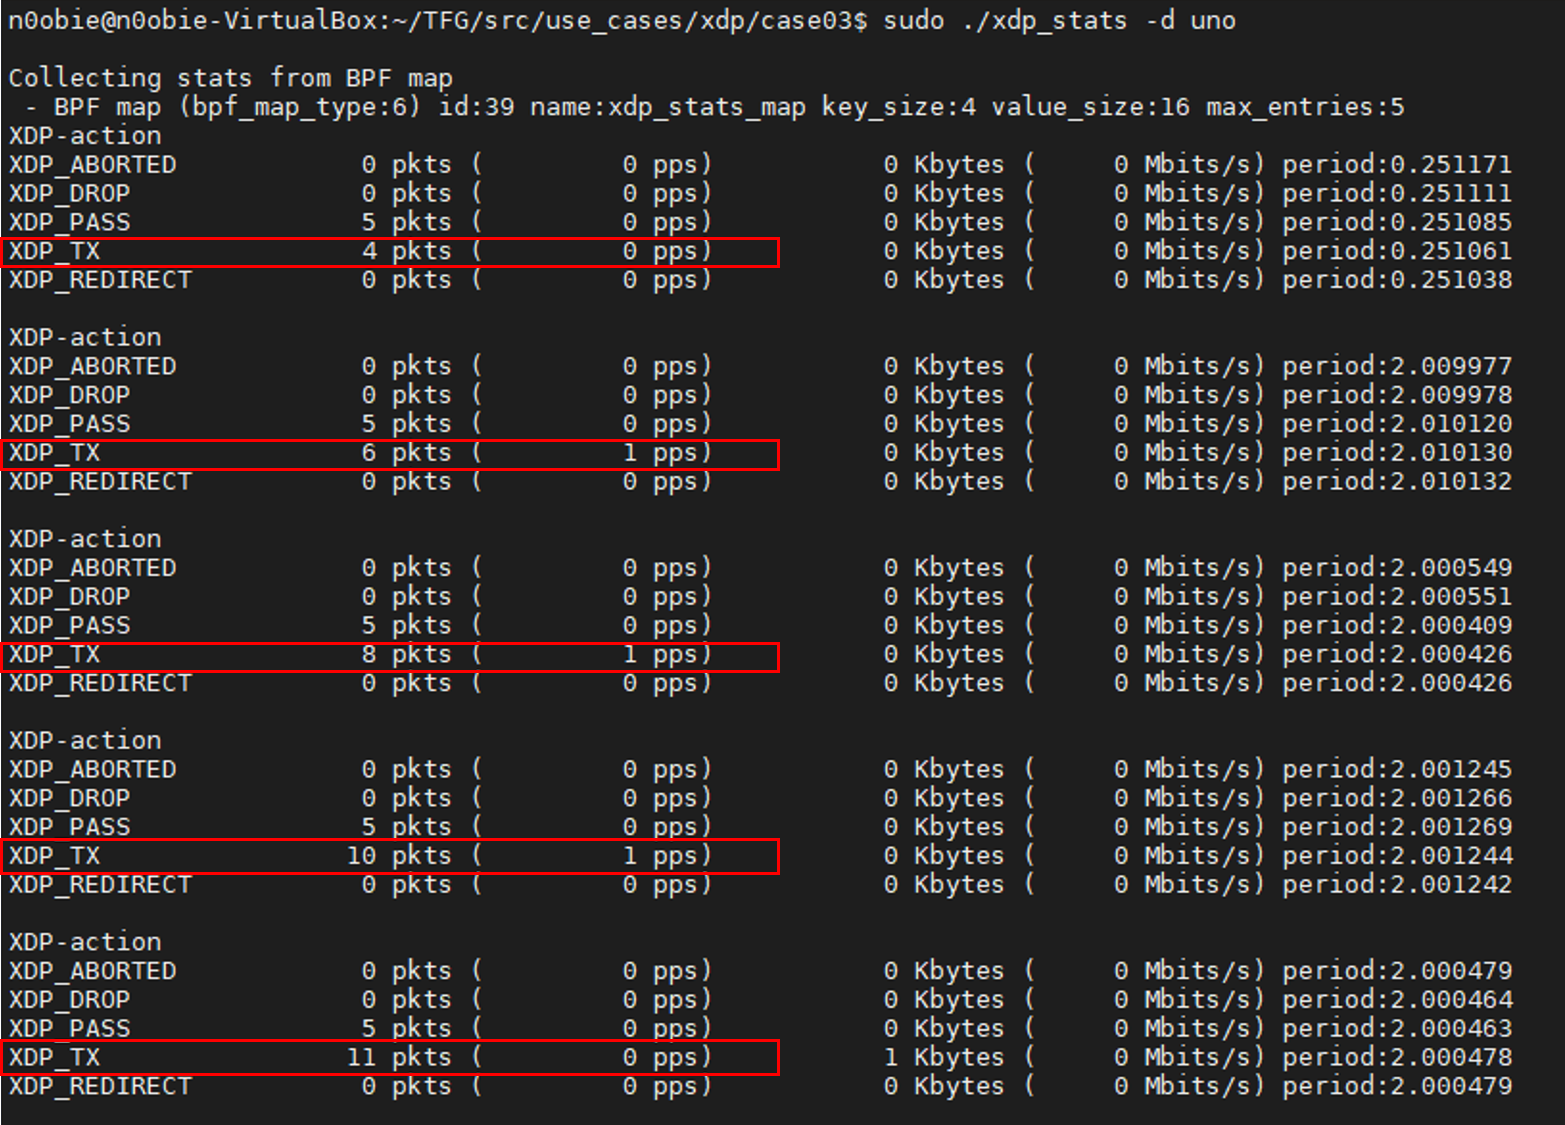
\includegraphics[width=11cm]{archivos/img/dev/xdp/case03/demo_case03_3_edited.png}
        \caption{Estadísticas de los códigos de retorno XDP}
        \label{fig:case03_xdp_ether_func_stats}
    \end{subfigure}
    \caption{Comprobación de funcionamiento del Case03 - XDP}
    \label{fig:case03_xdp_ether_func1}
\end{figure}

Si todo funciona correctamente se debería ver como los códigos de retorno mayormente empleados son los de \texttt{XDP\_TX} siempre y cuando no se haya detenido el ping  desde dentro de la \textit{Network Namespace}. Como se puede apreciar en la figura \ref{fig:case03_xdp_ether_func1}, el ping \fcolorbox{black}{green}{\rule{0pt}{2.5pt}\rule{2.5pt}{0pt}}\hspace{1mm} está siendo contestado correctamente por el programa \gls{xdp} dado que los códigos \texttt{XDP\_TX} van aumentando.\\
\par
De forma adicional, se va a comprobar cómo todos los pings que se manden desde dentro de la \textit{Network Namespace} \texttt{uno} serán contestados. Esto es así, ya que el programa \gls{xdp}, contestará todos los \texttt{ECHO-REQUEST} que le lleguen independientemente de si van dirigidos a él. En la figura \ref{fig:case03_xdp_ether_func2} se puede ver cómo funciona un ping \fcolorbox{black}{orange}{\rule{0pt}{2.5pt}\rule{2.5pt}{0pt}}\hspace{1mm} a una máquina inexistente. Para ello, se ha tenido que añadir una MAC inventada en la tabla ARP asociada a la IP a la cual vamos hacer ping  para que no se iniciara una resolución ARP. En el caso de que se iniciara una resolución ARP, el ping estaría bloqueado a la espera de completar una resolución ARP sobre una máquina inexistente. 

\begin{figure}[h]
    \centering
    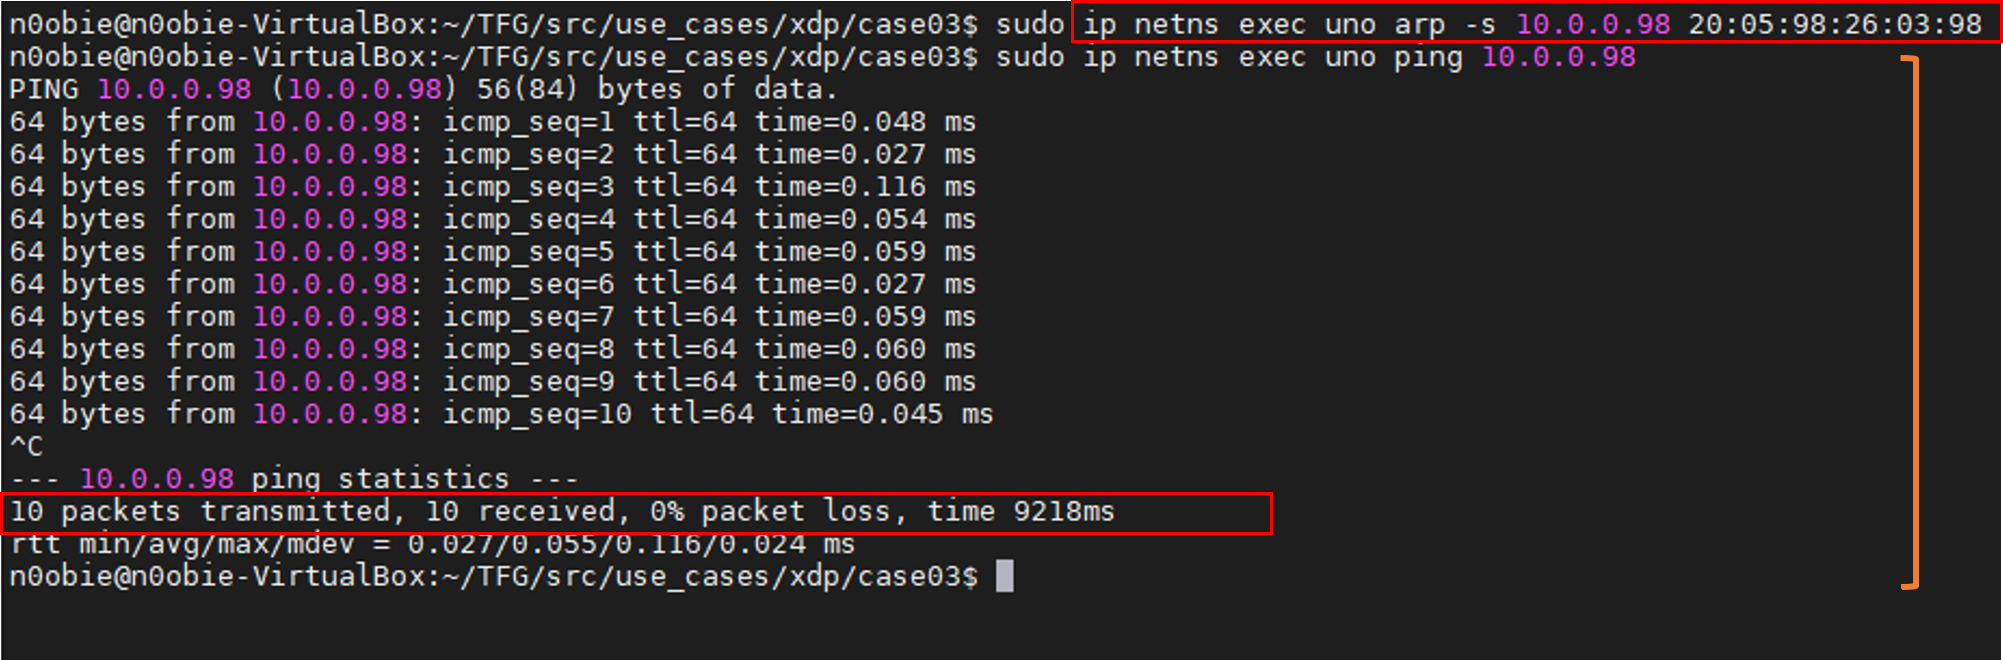
\includegraphics[width=14cm]{archivos/img/dev/xdp/case03/demo_case03_4_edited.png}
    \caption{Ping a máquina inexistente - XDP}
    \label{fig:case03_xdp_ether_func2}
\end{figure}

\subsection{Case04 - Layer 3 forwarding}
\label{xdp_ether_case04}

En este caso de uso se explorará como realizar forwarding de paquetes. En este punto, ya se ha revisado cómo filtrar por las cabeceras de los paquetes, analizarlos y establecer una lógica asociada a ese filtrado con los códigos de retorno \gls{xdp}. Una acción adicional a realizar con los paquetes será el forwarding. En \gls{xdp} vendrá implementado por códigos de retorno y por \textit{helpers} \gls{bpf} porque, como ya comentábamos en el case02 (\ref{xdp_ether_case02}), \gls{xdp} se termina traduciendo en \gls{bpf} (e\gls{bpf}), por lo que ciertas funciones, no todas, para trabajar con \gls{bpf} están disponibles a la hora de trabajar con \gls{xdp}.\\
\par

A lo largo de este caso de uso, se han explorado las distintas maneras para lograr el forwarding con \gls{xdp}. Se ha ido desde la manera más simple a la manera más robusta y, a su vez, compleja. Para que no haya diferencias entre las distintas formas de realizar el forwarding, se ha creado un mismo escenario donde se explorarán estas vías sin que existan diferencias inducidas por este. En el caso de uso anterior ya se estaba haciendo un forwarding, ya que, con el código \texttt{XDP\_TX} se realiza un forwarding hacia la interfaz por la cual se recibió dicho paquete. Pero, ¿cómo se hace un forwarding hacia otras interfaces? Leyendo la \textit{man-page} de los \textit{helpers} \gls{bpf} se han encontrado las funciones \texttt{bpf\_redirect()}, \texttt{bpf\_redirect\_map()}, las cuales, leyendo su descripción, serán la vía utilizada para abordar esta necesidad.

\begin{lstlisting}[language=C, style=C-color, caption={Helper BPF para realizar Forwarding - Case04},label=code:case04_xdp_ether_kernprog1]
    int bpf_redirect(u32 ifindex, u64 flags);

    int bpf_redirect_map(struct bpf_map *map, u32 key, u64 flags);
\end{lstlisting}


\vspace{0.5cm}
\textbf{Compilación}\\
\par

Para compilar el programa \gls{xdp} se ha dejado un Makefile preparado en este directorio al igual que en el case03 (\ref{xdp_ether_case03}), por lo que para compilarlo únicamente hay que seguir las indicaciones del bloque \ref{code:case04_xdp_ether_compilacion}.

\begin{lstlisting}[language= bash, style=Consola, caption={Compilación programa XDP - Case04},label=code:case04_xdp_ether_compilacion]
    # En caso de no haber entrado en el directorio asignado del caso de uso
    cd TFG/src/use_cases/xdp/case04
    
    # Hacemos uso del Makefile suministrado 
    sudo make
\end{lstlisting}
\vspace{0.5cm}

Podrá encontrar más información sobre el proceso de compilación de los programas \gls{xdp} en el case02 (\ref{xdp_ether_case02}).


\vspace{0.7cm}
\textbf{Puesta en marcha del escenario}\\
\par
Para comprobar el funcionamiento de los programas \gls{xdp} se hará uso de las \textit{Network Namespace} (más información en la sección \ref{namespaces}). Como ya se comentaba, para que no suponga una barrera de entrada el concepto de las \textit{Network Namespace}, se ha dejado escrito un script para levantar el escenario, y para su posterior limpieza. Es importante señalar que el script debe ser lanzado con permisos de root. Para levantar el escenario debemos ejecutar dicho script como se indica en el bloque \ref{code:case03_xdp_ether_escenario}. Para limpiar la máquina del escenario recreado anteriormente, se puede correr el mismo script indicándole ahora el parámetro \texttt{-c} (\textit{Clean}). En el peor de los casos, y si se cree que la limpieza se no se ha realizado de manera satisfactoria, se puede llevar a cabo un reinicio de la máquina consiguiendo así que todos los entes no persistentes (\gls{veth}, netns..) desaparezcan del equipo.

\begin{lstlisting}[language= bash, style=Consola, caption={Puesta en marcha del escenario - Case04},label=code:case04_xdp_ether_escenario]
    # Para levantar el escenario (Importante hacerlo con permisos de super usuario)
    sudo ./runenv.sh -i
    
    
    # Una vez finalizado la comprobación del caso de uso, limpiaremos nuestra maquina:
    sudo ./runenv.sh -c
\end{lstlisting}
\vspace{0.5cm}

%%%%%%%%%%%%%%%%%%%%%%%%%%%%%%%%%%%%%%%%%%%%%%%%%%%%%%%%%%%%%%%%%%%%%%%%%%%%%%%%%%%%

\subsubsection{Hardcoded forwarding}
\label{xdp_ether_case04_hard}

La primera forma de implementación del forwarding es lo que denominaremos como Hardcoded forwarding, dado que es necesario hardcodear\footnote{Hardcodear: perder flexibilidad y/o prolijidad dejando valores y/o comportamientos fijos en el código del programa.} información de forwarding en el propio programa \gls{xdp}. El escenario levantado se puede apreciar en la figura \ref{fig:case04_xdp_ether_scenario1}, está compuesto de dos \textit{Network Namespace} (\texttt{uno} y \texttt{dos}), y de dos pares de \gls{veth}s (\texttt{veth0} -- \texttt{uno} y \texttt{veth0} -- \texttt{dos}) las cuales se utilizarán para comunicar las dos \textit{Network Namespaces} entre sí, a través del la \textit{Network Namespace} por defecto. En este caso el forwarding lo haremos desde la interfaz \texttt{dos} hacia la interfaz \texttt{uno}.


% figura escenario
\begin{figure}[ht]
    \centering
    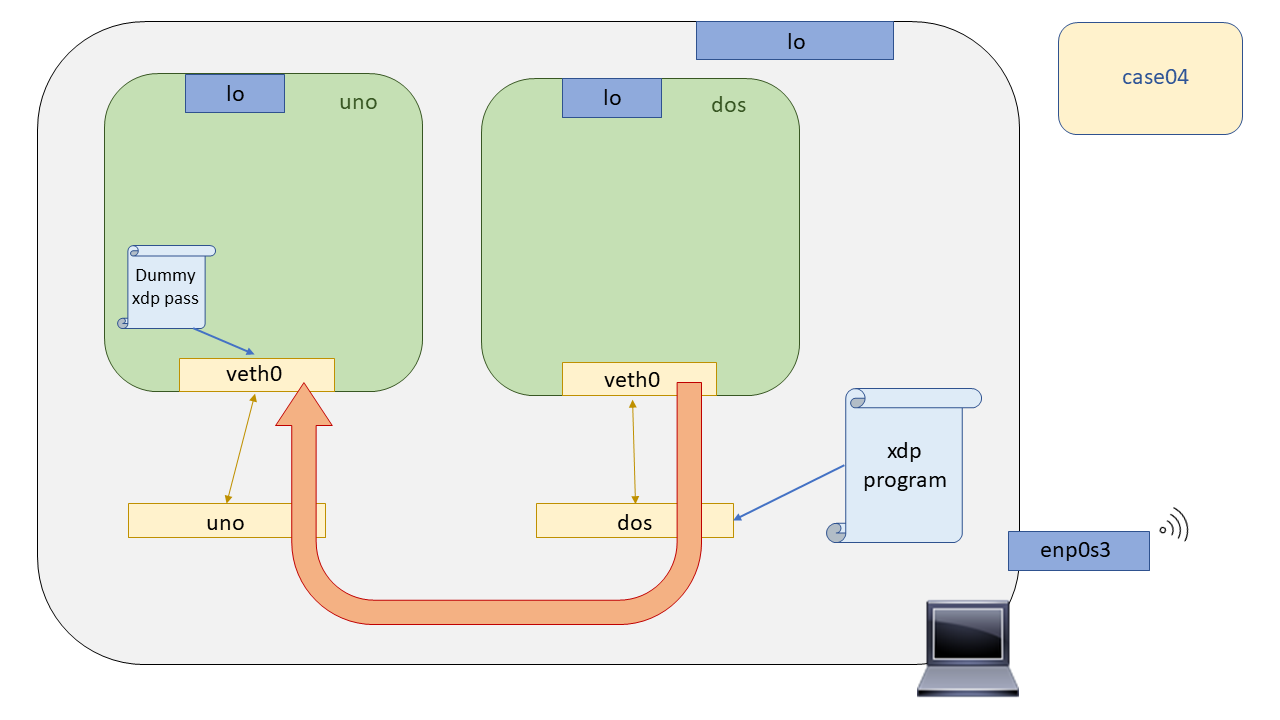
\includegraphics[width=16cm]{archivos/img/dev/xdp/case04/scenario_01.png}
    \caption{Escenario cableado Hardcoded forwarding del Case04 - XDP}
    \label{fig:case04_xdp_ether_scenario1}
\end{figure}


\vspace{0.5cm}
\textbf{Carga del programa XDP}\\
\par

Antes de realizar la carga del programa se deben obtener \textbf{dos datos}, la \textit{ifindex} de la interfaz uno a la cual se van a mandar los paquetes generados desde el interior de la \textit{Network Namespace} \texttt{dos}, y la MAC de la interfaz interna de la \textit{Network Namespace} \texttt{uno}, ya que será necesario que los paquetes que se dirijan a la interfaz \texttt{uno} lleven como MAC destino la de la \texttt{veth0}, para que así los paquetes no sean descartados.\\
\par
Una vez se tengan estos datos anotados se abrirá el programa \gls{xdp} (\texttt{*.c}) con cualquier editor de texto, se irá a la declaración de variables y se hardcodeará como se puede ver en el bloque \ref{code:case04_xdp_ether_kernprog2} tanto el \textit{ifindex} como la MAC.
\par

\begin{lstlisting}[language=C, style=C-color, caption={Ejemplo MAC e Ifindex - Case04},label=code:case04_xdp_ether_kernprog2]
    /*  Para un ifindex: 6 y una MAC: 9A:DE:AF:EC:18:6E */

    ...
    
    unsigned char dst[ETH_ALEN + 1] = {0x9a,0xde,0xaf,0xec,0x18,0x6e, '\0'} ;
    unsigned ifindex = 6; 

    ...
\end{lstlisting}
\vspace{0.5cm}
Una vez que se tenga hardcodeado los datos para realizar el forwarding se debe recompilar el programa \gls{xdp} para que el \textit{bytecode} que se ancle a la interfaz dos haga correctamente el forwarding. Por ello, simplemente se tiene que hacer un \textit{make} nuevamente.\\
\par
Por lo tanto, teniendo todo preparado es hora de anclar de nuevo el programa \gls{xdp}. Recordemos que por el estar trabajando con interfaz \gls{veth}s se debe anclar un \textit{dummy program}\footnote{\url{https://netdevconf.info/0x13/session.html?talk-veth-xdp}} en el extremo donde se vayan a recibir los paquetes.
\begin{lstlisting}[language= bash, style=Consola, caption={Carga del programa XDP Hardcoded forwarding - Case04},label=code:case04_xdp_ether_load1]
    # Entramos a la Network Namespace "uno" y anclamos el dummy program a la interfaz veth0
    sudo ip netns exec uno ./xdp_loader -d veth0 -F --progsec xdp_pass
    
    # Acto seguido, anclamos el programa a la interfaz "dos" como ya comentábamos antes
    sudo ./xdp_loader -d dos -F --progsec xdp_case04
\end{lstlisting}

\vspace{0.5cm}
\textbf{Comprobación del funcionamiento}\\
\par
La comprobación de funcionamiento de este programa \gls{xdp} es bastante básica, se va a generar paquetes desde el interior de la \textit{Network Namespace}  \texttt{dos} hacia la \gls{veth} interna de la \textit{Network Namespace} \texttt{uno}. Si todo funciona correctamente deberían llegar los paquetes en el sentido dispuesto del forwarding hardcodeado, sería una comunicación unidireccional. Para ello se abrirán tres terminales, en cada una de ellas se llevará a cabo una tarea. Ver bloque \ref{code:case04_xdp_ether_func1}, donde se indican todos los comandos necesarios para comprobar el funcionamiento del Hardcoded forwarding.

\begin{lstlisting}[language= bash, style=Consola, caption={Comprobación del funcionamiento Hardcoded forwarding - Case04},label=code:case04_xdp_ether_func1]
    # En esta terminal generaremos el ping hacia la interfaz de la Network Namespace "uno" desde la Network Namespace "dos"
    [Terminal:1] sudo ip netns exec dos ping {IP_veth0_uno}
    
    # En esta terminal pondremos a un sniffer a escuchar los paquetes que nos lleguen dentro de la Network Namespace "dos"
    [Terminal:2] sudo ip netns exec uno tcpdump -l
    
    # Por último, opcionalmente, podemos ejecutar el programa que actuaba como recolector de estadísticas sobre los códigos de retorno XDP
    [Terminal:3] sudo ./xdp_stats -d dos
\end{lstlisting}

% figura escenario
\begin{figure}[ht]
    \centering
    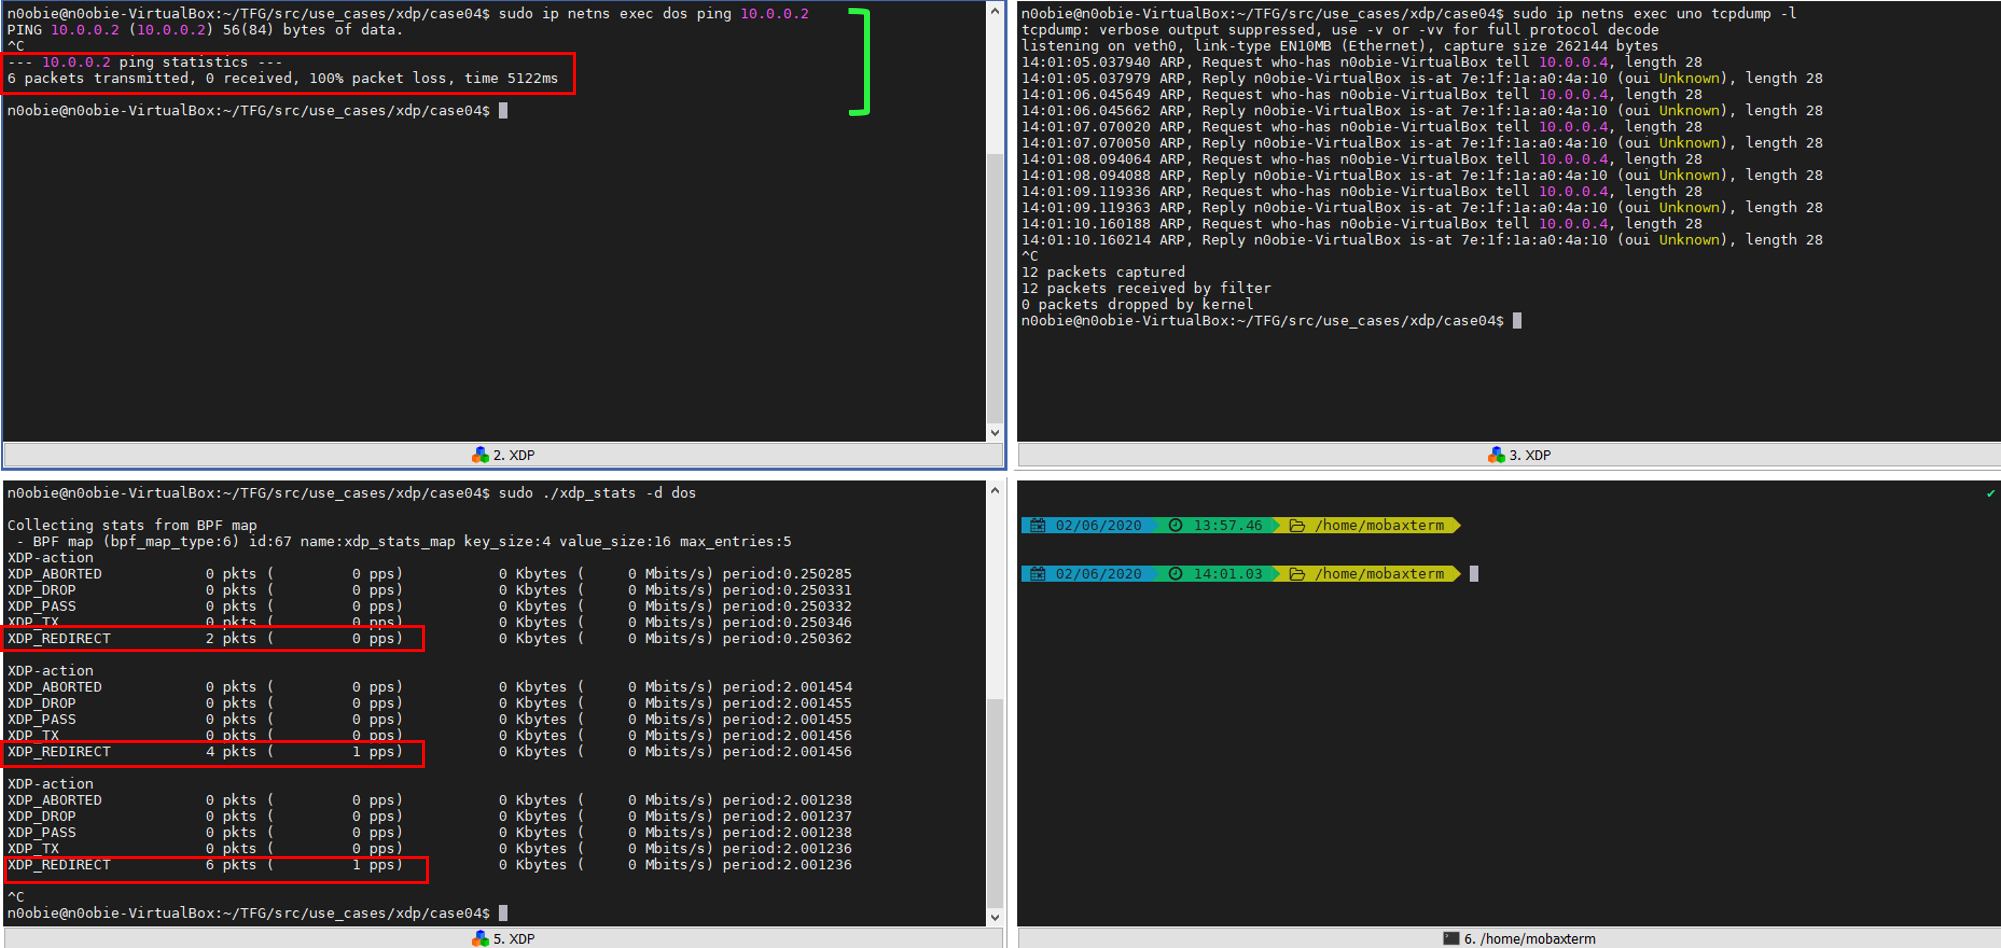
\includegraphics[width=15.5cm]{archivos/img/dev/xdp/case04/demo_case04_hard_1_edited.png}
    \caption{Comprobación de funcionamiento Hardcoded forwarding del Case04 - XDP}
    \label{fig:case04_xdp_ether_func1_b}
\end{figure}

Como se puede apreciar en la figura \ref{fig:case04_xdp_ether_func1_b}, el ping \fcolorbox{black}{green}{\rule{0pt}{2.5pt}\rule{2.5pt}{0pt}}\hspace{1mm} no llega a completarse. Esto se debe a que al implementar una comunicación unidireccional, el ping se queda bloqueado en la resolución ARP. Se puede corroborar este funcionamiento atendiendo a los códigos de retorno \gls{xdp}, \texttt{XDP\_REDIRECT}, como van en aumento debido a los reenvíos de los paquetes ARP-Request de una interfaz a la otra y por la escucha de tcpdump en la terminal superior derecha. 
%%%%%%%%%%%%%%%%%%%%%%%%%%%%%%%%%%%%%%%%%%%%%%%%%%%%%%%%%%%%%%%%%%%%%%%%%%%%%%%%%%%%

\subsubsection{Semi-Hardcoded forwarding (BPF maps)}

La segunda forma de implementar el forwarding se denominará Semi-Hardcoded forwarding, ya que la información irá hardcodeada, pero no en el propio programa \gls{xdp}, sino, en los mapas \gls{bpf}. El escenario levantado se puede apreciar en la figura \ref{fig:case04_xdp_ether_scenario2}, está compuesto de dos \textit{Network Namespace} (\texttt{uno} y \texttt{dos}), y de dos pares de \gls{veth}s (\texttt{veth0} -- \texttt{uno} y \texttt{veth0} -- \texttt{dos}) las cuales se utilizarán para comunicar las dos \textit{Network Namespaces} entre sí, a través del la \textit{Network Namespace} por defecto. En este caso el forwarding se hará desde la interfaz \texttt{dos} hacia la interfaz \texttt{uno} y viceversa, por lo que la comunicación será bidireccional.

% figura escenario
\begin{figure}[ht]
    \centering
    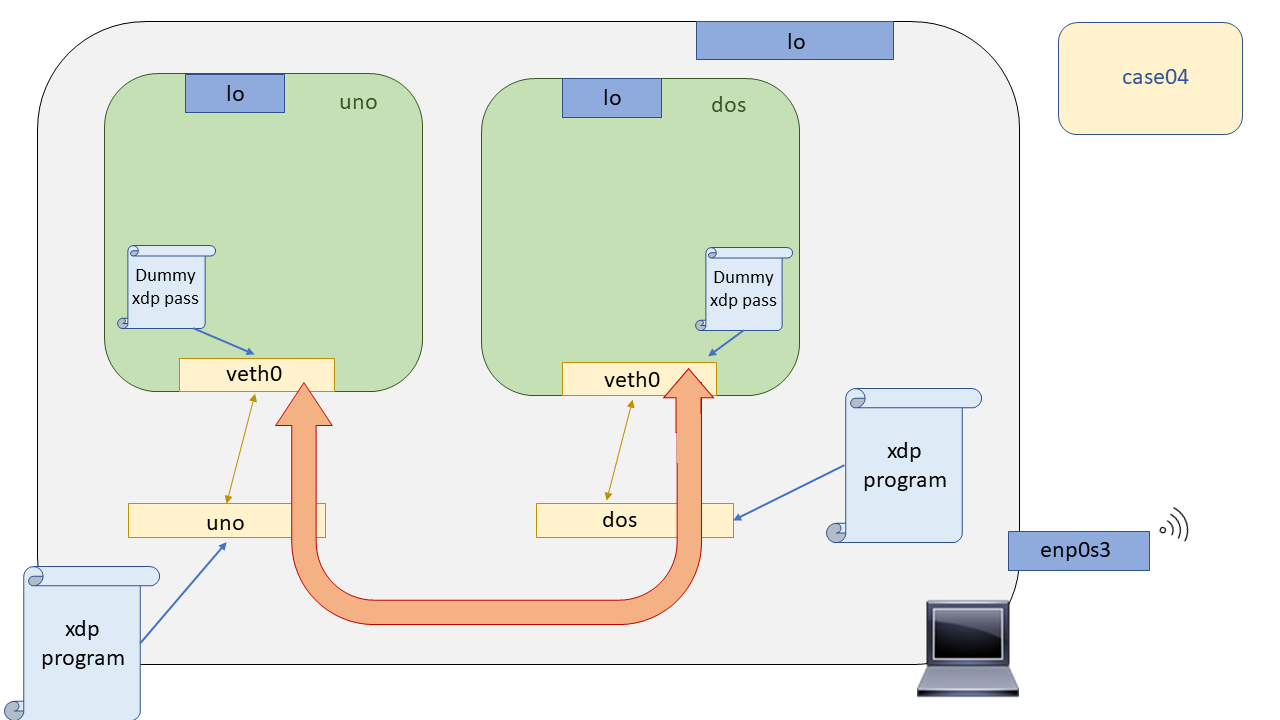
\includegraphics[width=14cm]{archivos/img/dev/xdp/case04/scenario_02.png}
    \caption{Escenario cableado Semi-Hardcoded forwarding del Case04 - XDP}
    \label{fig:case04_xdp_ether_scenario2}
\end{figure}

\vspace{1cm}
\textbf{Carga del programa XDP}\\
\par
Esta manera de hacer el forwarding no requiere de hardcodear datos en el propio programa \gls{xdp} que irá al Kernel, si no, que se usarán los mapas \gls{bpf} como medio para guardar datos de forwarding como son las \textit{ifindex} y las MAC destino desde espacio de usuario. De esta forma, posteriormente el programa anclado en el Kernel sea capaz de leer los mapas, obtener la información de forwarding y realizarlo en base a la información percibida de los mapas \gls{bpf}.\\
\par

De nuevo, y como en este caso la comunicación será bidireccional se debe anclar dos \textit{dummy program} en los dos extremos donde van a llegar los paquetes, si no se está al tanto de esta limitación vuelva a la subsección (\ref{xdp_ether_case04_hard}) donde se menciona la limitación.\\
\par

Es importante señalar que los programas anclados previamente deben ser retirados, por lo que una opción sería hacer un \textit{clean} del escenario haciendo uso del script dado ( \texttt{sudo ./runenv.sh -c}) y empezar de nuevo.\\
\par
\begin{lstlisting}[language= bash, style=Consola, caption={Carga del programa XDP Semi-Hardcoded forwarding - Case04},label=code:case04_xdp_ether_load2]
    # Entramos en cada Network Namespace y anclamos los "dummy programs"
    sudo ip netns exec uno ./xdp_loader -d veth0 -F --progsec xdp_pass
    sudo ip netns exec dos ./xdp_loader -d veth0 -F --progsec xdp_pass
    
    # Anclamos el programa XDP en cada interfaz para conseguir un comunicación bidireccional 
    sudo ./xdp_loader -d uno -F --progsec xdp_case04_map
    sudo ./xdp_loader -d dos -F --progsec xdp_case04_map
    
    # Almacenamos la información necesaria para realizar el forwarding 
    src="uno"
    dest="dos"
    src_mac=$(sudo ip netns exec $src cat /sys/class/net/veth0/address)
    dest_mac=$(sudo ip netns exec $dest cat /sys/class/net/veth0/address)
     
    # Populamos los mapas BPF con la información útil para llevar a cabo el forwarding en ambas direcciones
    ./prog_user -d $src -r $dest --src-mac $src_mac --dest-mac $dest_mac
    ./prog_user -d $dest -r $src --src-mac $dest_mac --dest-mac $src_mac
\end{lstlisting}


\vspace{1cm}
\textbf{Comprobación del funcionamiento}\\
\par
La comprobación de funcionamiento de este programa puede ser llevada a cabo desde un extremo u otro debido a que, si todo funciona correctamente, existirá una comunicación bidireccional. Por lo que, en este caso se harán las pruebas desde la \textit{Network namespace} \texttt{uno} hacia la \texttt{dos}.\\
\par
Como se puede apreciar en la figura \ref{fig:case04_xdp_ether_func2}, existe una comunicación bidireccional ya que el ping \fcolorbox{black}{orange}{\rule{0pt}{2.5pt}\rule{2.5pt}{0pt}}\hspace{1mm} se ejecuta con normalidad. Además, en la subfigura \ref{fig:case04_xdp_ether_func2_stats} se puede ver como los códigos de retorno \gls{xdp} de forwarding van aumentando, por lo que el programa \gls{xdp} está funcionando según lo previsto.

\begin{figure}[h]
    \centering
    \begin{subfigure}[b]{\textwidth}
    	\centering
        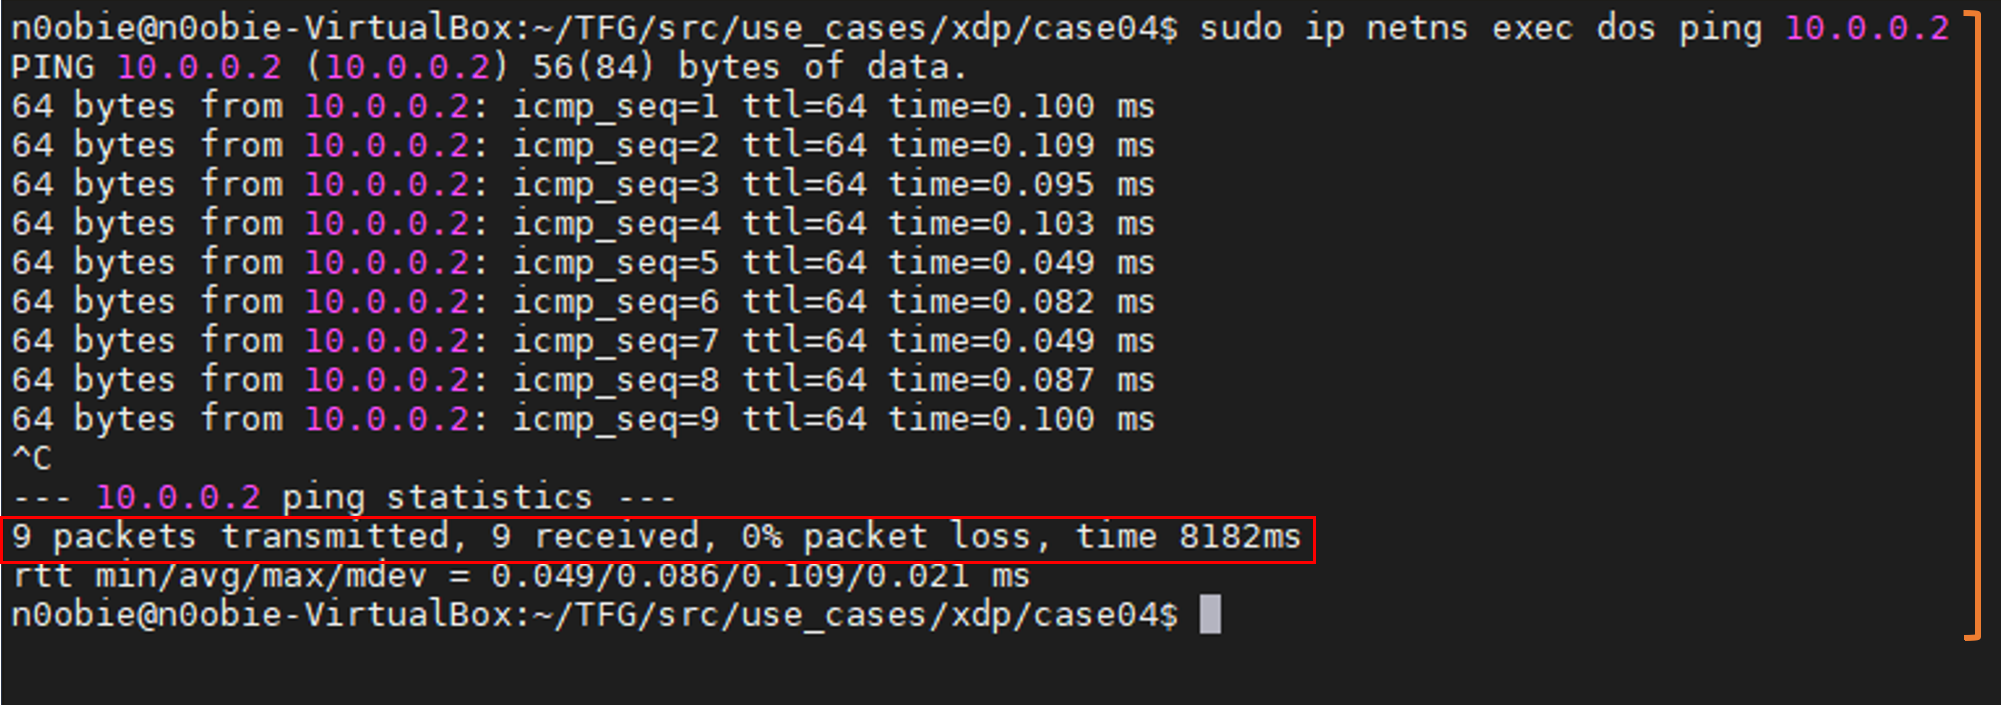
\includegraphics[width=11cm]{archivos/img/dev/xdp/case04/demo_case04_semihard_2_edited.png}
        \caption{Ejecución de ping hacia la interfaz con el programa XDP}
        \label{fig:case04_xdp_ether_func2_ping}
    \end{subfigure}
    \par\bigskip
    \begin{subfigure}[b]{\textwidth}
    	\centering
        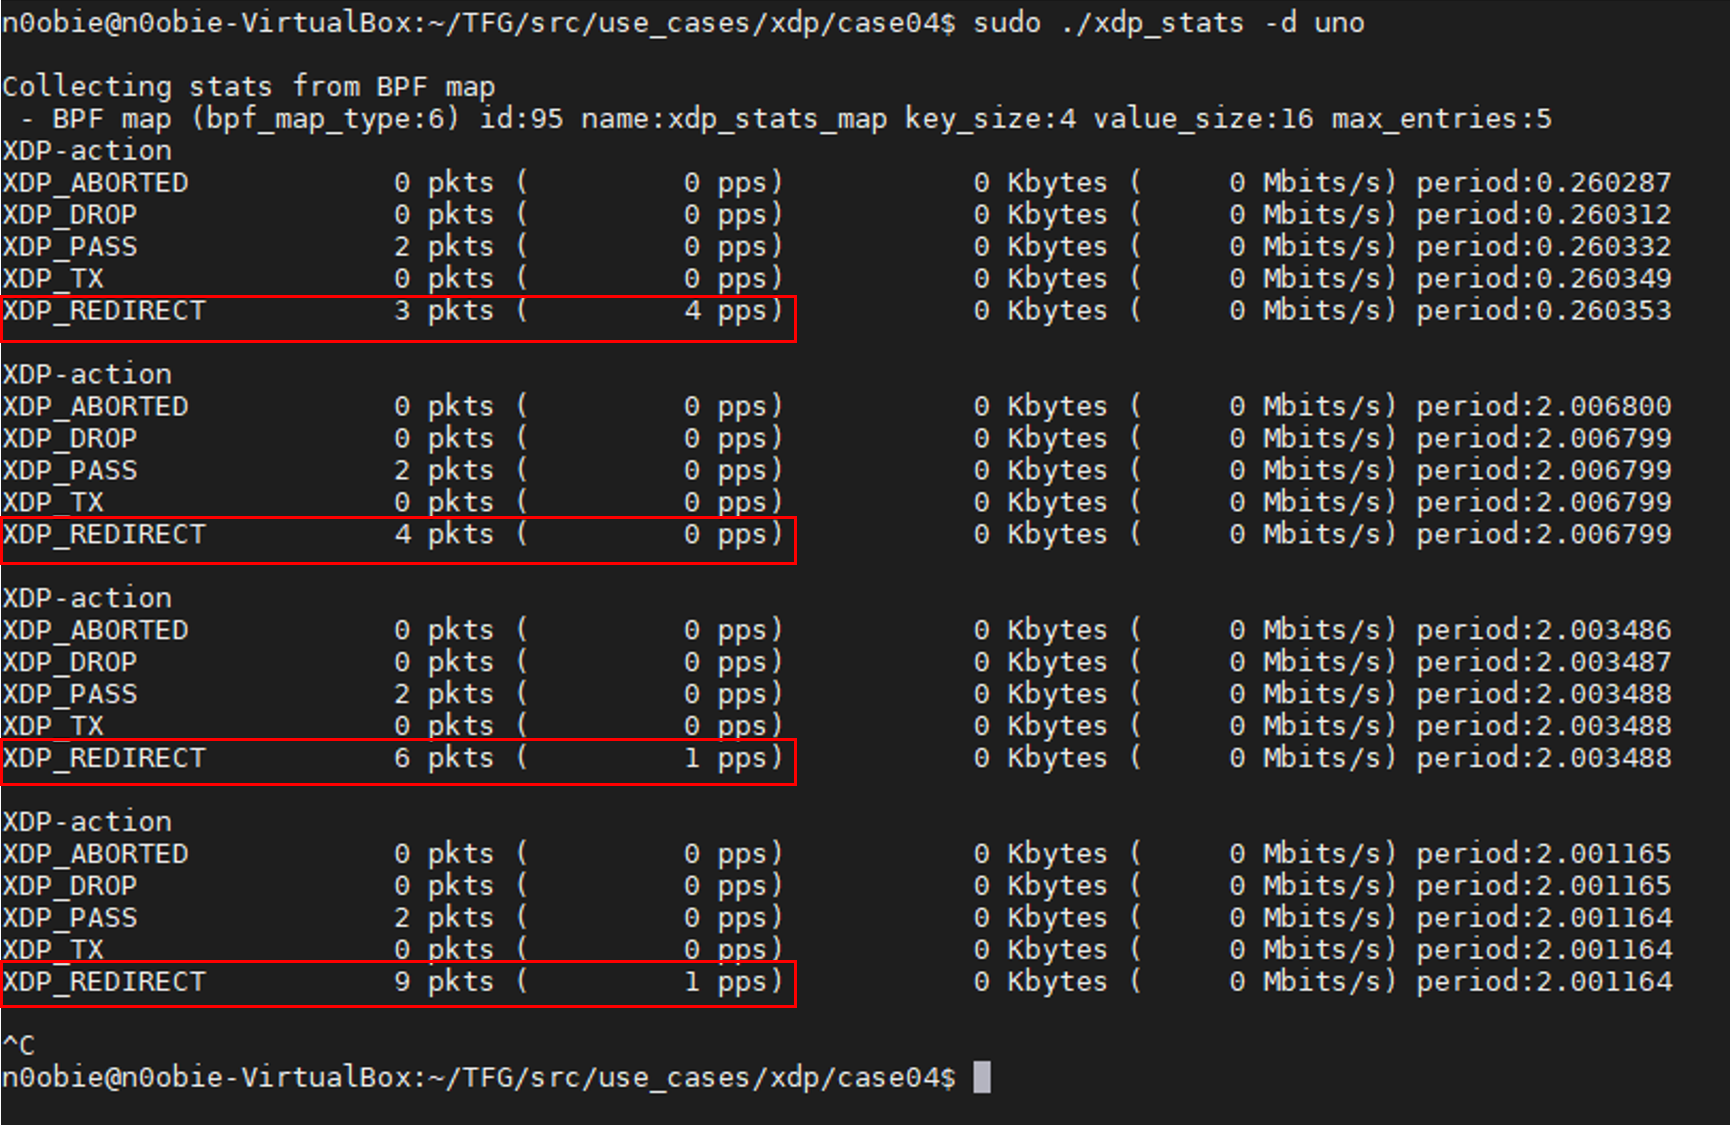
\includegraphics[width=14cm]{archivos/img/dev/xdp/case04/demo_case04_semihard_3_edited.png}
        \caption{Estadísticas de los códigos de retorno XDP}
        \label{fig:case04_xdp_ether_func2_stats}
    \end{subfigure}
    \caption{Comprobación de funcionamiento Semi-Hardcoded forwarding del Case04 - XDP}
    \label{fig:case04_xdp_ether_func2}
\end{figure}

% \todo{Cambiar este bloque de código por una imagen ya que es un resultado}
% \begin{lstlisting}[language= bash, style=Consola, caption={Comprobación del funcionamiento Semi-Hardcoded forwarding - Case04},label=code:case04_xdp_ether_func2]
%     # Hacemos un ping desde el interior de la Network namespace "uno" hacia la veth0 de la Network namespace "dos"
%     ping  {IP_veth_dos} [ y viceversa..]
    
%     # Comprobamos con el recolector de estadísticas que se están produciendo XDP_REDIRECT
%     sudo ./xdp_stats -d uno
    
%     ó
    
%     sudo ./xdp_stats -d dos
% \end{lstlisting}



%%%%%%%%%%%%%%%%%%%%%%%%%%%%%%%%%%%%%%%%%%%%%%%%%%%%%%%%%%%%%%%%%%%%%%%%%%%%%%%%%%%%
\subsubsection{Forwarding auto (Kernel FIBs)}

La tercera forma de hacer forwarding hace referencia al forwarding automático, esto es debido a que no habrá ningún tipo de información de forwarding hardcodeada en el programa \gls{xdp}, la información se obtendrá del propio \textit{stack} de red trabajando de forma cooperativa con éste. El escenario sobre el cual se trabajará será el mismo que el anterior por lo que únicamente es necesario preocuparse de limpiar el escenario de los programas \gls{xdp} anteriormente anclados a cada interfaz para que no interfieran con los nuevos programas \gls{xdp} que se van anclar.\\
\par
En este caso, se va a ir un paso más allá y el forwarding será automático, es decir, no se hardcodeará ningún tipo de información para hacer el forwarding a los paquetes. Pero, entonces: ¿cómo se sabrá a dónde hay que mandar los paquetes? Esta información se conseguirá del \textit{stack} de red del Kernel de Linux el cual tiene una FIB (\textit{Forwarding Information Base}) con reglas muy útiles las cuales se pueden sacar partido. \\
\par
Por lo que, se realizará una consulta a la FIB con el \textit{helper} \texttt{bpf\_fib\_lookup()} para obtener información de forwarding desde el propio \textit{stack} de red, este es un claro ejemplo donde la cooperación con el \textit{stack} de red hace que el programa \gls{xdp} sea más robusto e independiente del espacio de usuario.

% figura escenario
\begin{figure}[ht]
    \centering
    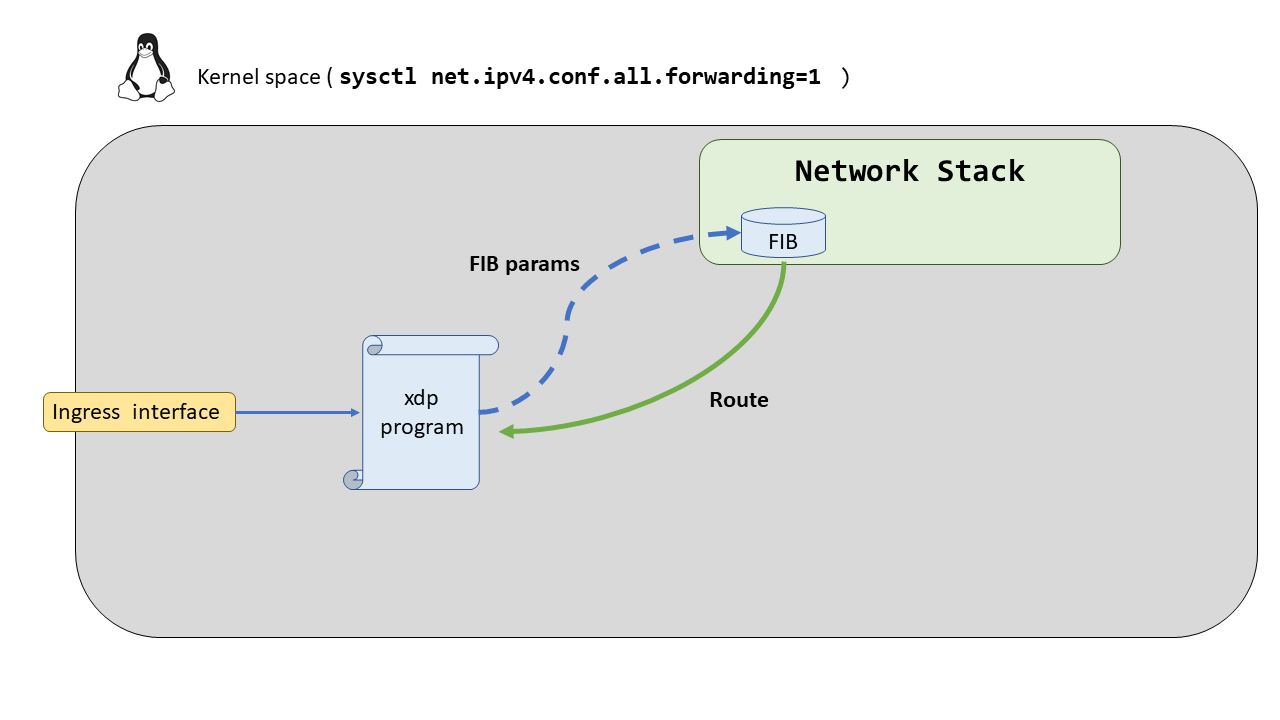
\includegraphics[width=16cm]{archivos/img/dev/xdp/case04/scenario_03.png}
    \caption{Escenario cableado Forwarding auto del Case04 - XDP}
    \label{fig:case04_xdp_ether_scenario3}
\end{figure}
\newpage
\vspace{1cm}
\textbf{Carga del programa XDP}\\
\par
Para la carga del programa \gls{xdp} se deberá primero habilitar el forwarding en nuestro Kernel, acto seguido se anclarán los \textit{dummy program} y por último, se anclarán anclar los programas \gls{xdp} en ambas interfaces tanto \texttt{uno} como \texttt{dos} para conseguir que la comunicación sea bidireccional.
\vspace{0.5cm}

\begin{lstlisting}[language= bash, style=Consola, caption={Carga del programa XDP Forwarding auto - Case04},label=code:case04_xdp_ether_load3]
    # Habilitamos el forwarding 
    sudo sysctl net.ipv4.conf.all.forwarding=1
    
    # Anclamos los programas XDP a cada interfaz 
    sudo ./xdp_loader -d uno -F --progsec xdp_case04_fib
    sudo ./xdp_loader -d dos -F --progsec xdp_case04_fib
    
    # Ahora añadimos a cada interfaz destino su "dummy program"
    sudo ip netns exec uno ./xdp_loader -d veth0 -F --progsec xdp_pass
    sudo ip netns exec dos ./xdp_loader -d veth0 -F --progsec xdp_pass
    
    # Habilitamos los ifindex 
    sudo ./prog_user -d uno
    sudo ./prog_user -d dos
\end{lstlisting}

\vspace{1cm}

\textbf{Comprobación del funcionamiento}\\
\par
La comprobación de funcionamiento de este programa puede ser llevada a cabo desde un extremo u otro debido a que, si todo funciona correctamente, existirá una comunicación bidireccional y completamente automática ya que no ha almacenado ningún tipo de información en los programas anclados. Por lo que, se harán las pruebas desde la \textit{Network namespace} \texttt{uno} hacia la \texttt{dos}. Como se puede apreciar en la figura \ref{fig:case04_xdp_ether_func3}, atendiendo al funcionamiento del ping \fcolorbox{black}{yellow}{\rule{0pt}{2.5pt}\rule{2.5pt}{0pt}}\hspace{1mm}, hay una perfecta comunicación entre ambas \textit{Network namespaces}, por lo que el programa está tomando correctamente las rutas de la FIB. \\

% \todo{Cambiar este bloque de código por una imagen ya que es un resultado}
\begin{lstlisting}[language= bash, style=Consola, caption={Comprobación del funcionamiento Forwarding auto - Case04},label=code:case04_xdp_ether_func3]
    # Hacemos un ping desde el interior de la Network namespace "uno" hacia la veth0 de la Network namespace "dos"
    ping  {IP_veth_dos} [ y viceversa..]
    
    # Comprobamos con el recolector de estadísticas que se están produciendo XDP_REDIRECT
    sudo ./xdp_stats -d uno

\end{lstlisting}

\newpage

\begin{figure}[h]
    \centering
    \begin{subfigure}[b]{\textwidth}
    	\centering
        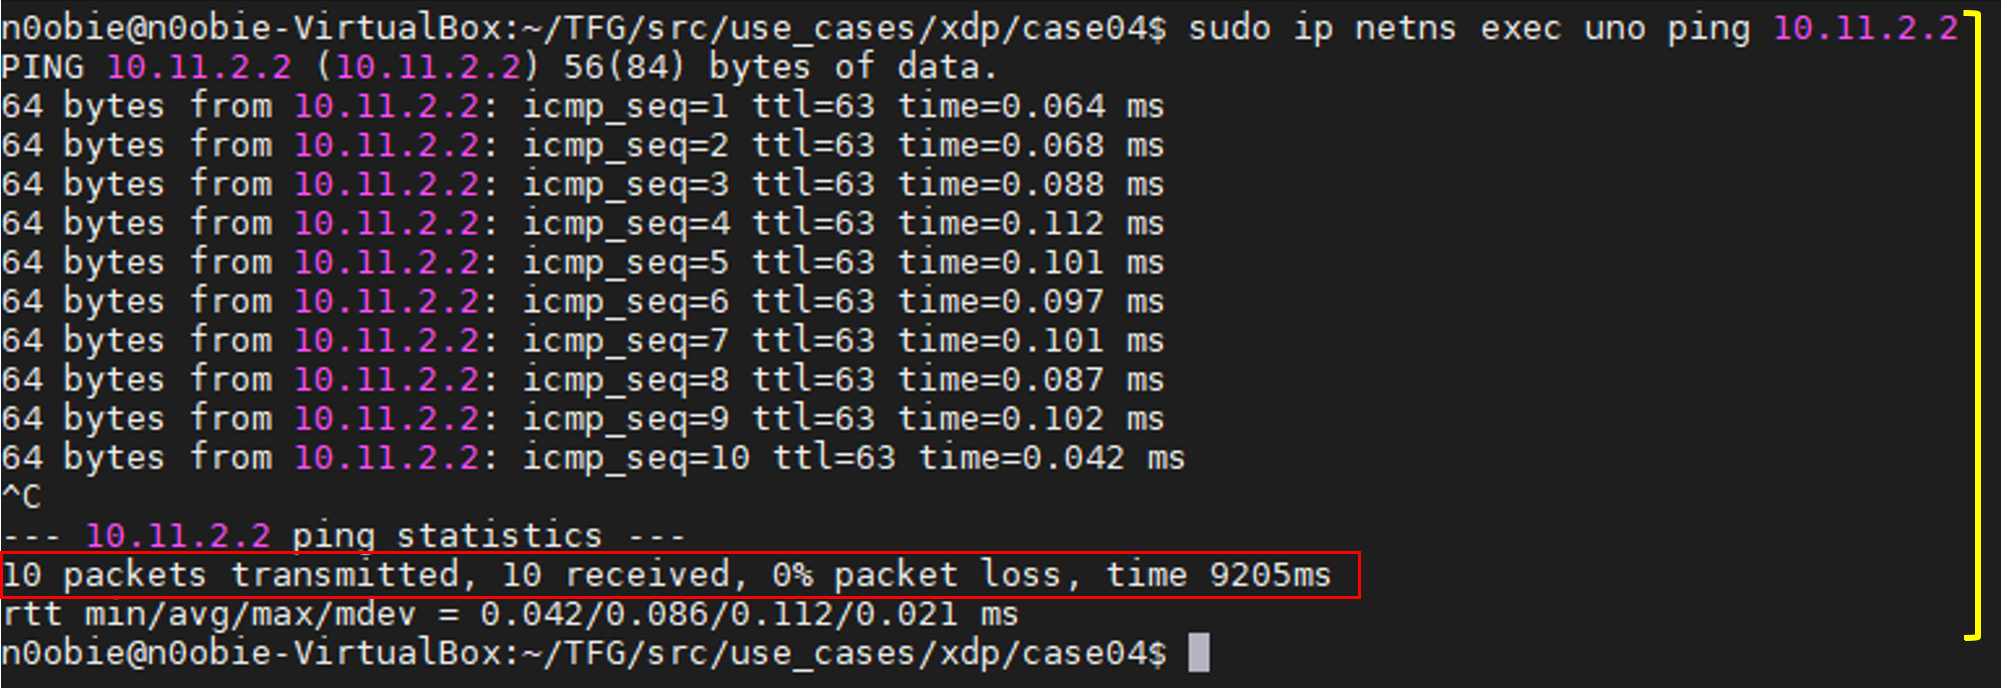
\includegraphics[width=13cm]{archivos/img/dev/xdp/case04/demo_case04_auto_2_edited.png}
        \caption{Ejecución de ping hacia la interfaz con el programa XDP}
        \label{fig:case04_xdp_ether_func3_ping}
    \end{subfigure}
    \par\bigskip
    \begin{subfigure}[b]{\textwidth}
    	\centering
        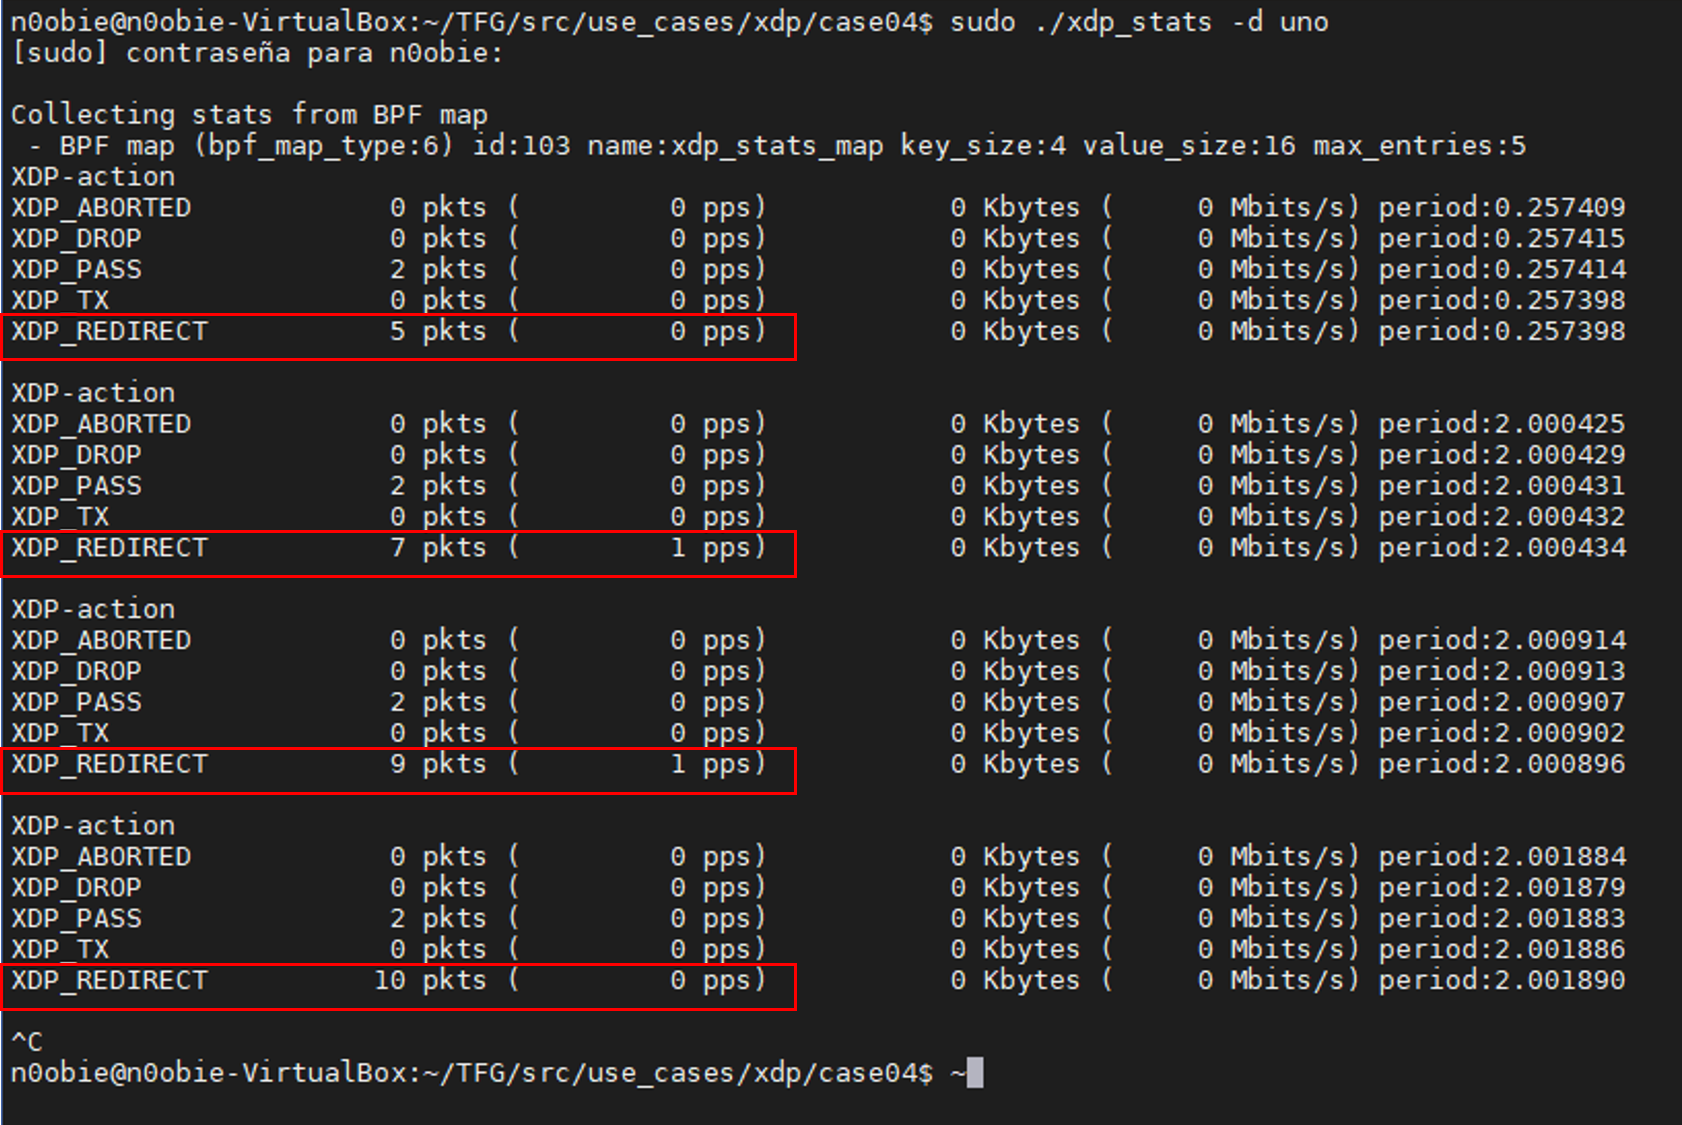
\includegraphics[width=14cm]{archivos/img/dev/xdp/case04/demo_case04_auto_3_edited.png}
        \caption{Estadísticas de los códigos de retorno XDP}
        \label{fig:case04_xdp_ether_func3_stats}
    \end{subfigure}
    \caption{Comprobación de funcionamiento Forwarding auto del Case04 - XDP}
    \label{fig:case04_xdp_ether_func3}
\end{figure}
\subsection{Case05 - Broadcast}
\label{xdp_ether_case05}

Por último, en este caso de uso se explorará la capacidad de reenvío a multiples interfaces de \gls{xdp}. Por ello, se ha intentado replicar un escenario básico de broadcast con \textit{Network Namespaces}. Se ha planteado hacer uso de la herramienta arping para emular una resolución ARP, generando paquetes ARP-Request. Dichos paquetes llevarán su MAC destino todo a \texttt{FF:FF:FF:FF:FF:FF} y su dominio de difusión englobaría todos aquellos nodos de la red que operen hasta capa 2. Como por ejemplo un hub, o un switch. En la figura \ref{fig:case05_xdp_ether_scenario1} se puede encontrar el escenario a recrear en este caso de uso.\\
\par
% figura escenario
\begin{figure}[ht]
    \centering
    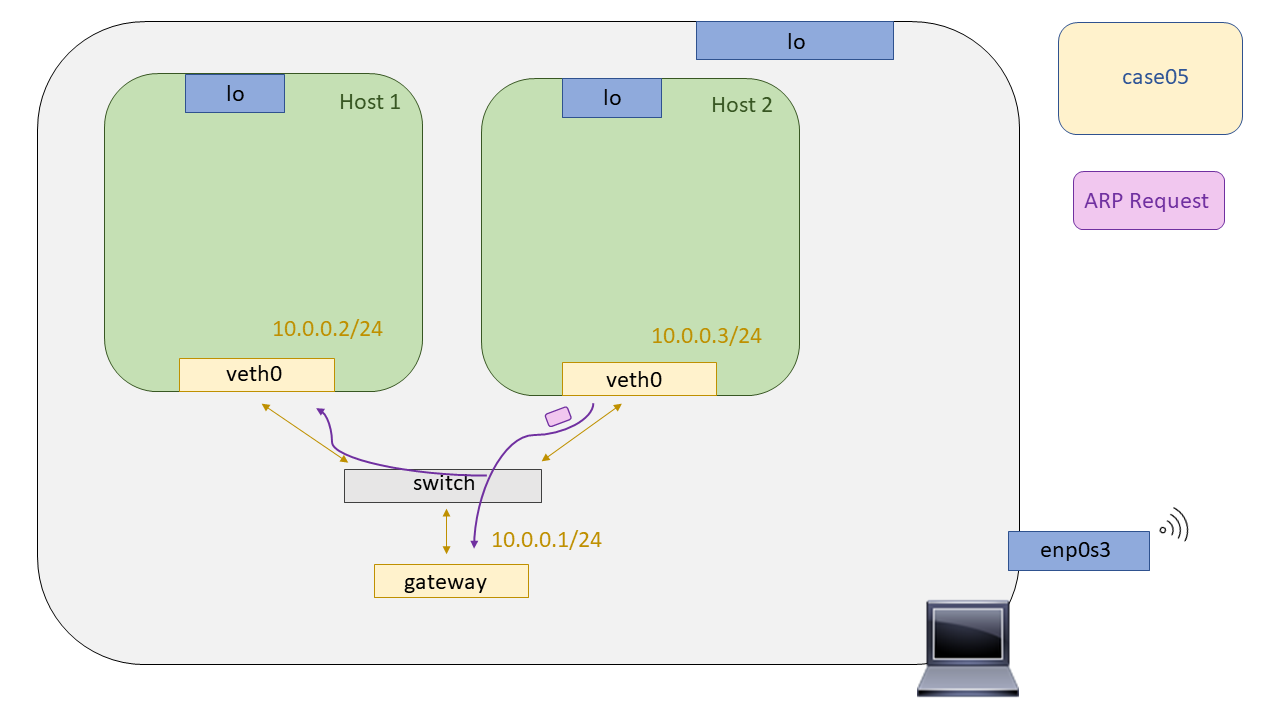
\includegraphics[width=14cm]{archivos/img/dev/xdp/case05/scenario_01.png}
    \caption{Escenario a recrear del Case05 - XDP}
    \label{fig:case05_xdp_ether_scenario1}
\end{figure}

El escenario propuesto para emular dicho escenario ha sido el siguiente (Ver figura \ref{fig:case05_xdp_ether_scenario2}). Este estaría compuesto de tres \textit{Network Namespaces} replicando así cada una de ellas un nodo independiente de la red, después, para intercomunicar cada ``nodo" de la red, se ha hecho uso de \gls{veth}s. El supuesto switch será la \textit{Network Namespace} llamada \texttt{switch}, la cual requerirá de un programa \gls{xdp} para poder actual como tal, ya que de no ser así sus interfaces tendrán todo el \textit{stack} de red de Linux por encima de ellas. Es decir, el nodo implementará todas las capas del modelo TCP/IP (DoD), replicando así la funcionalidad de un hipotético host y no actuando como un switch.\\
\par

% figura escenario
\begin{figure}[ht]
    \centering
    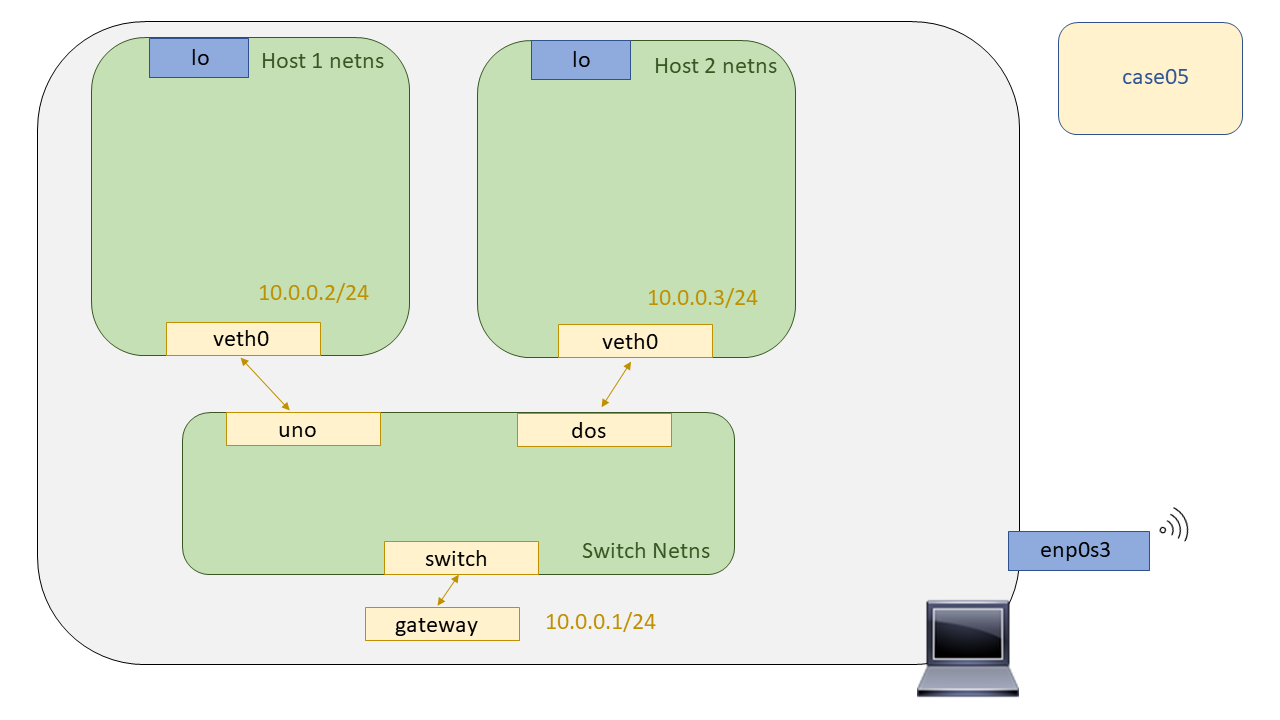
\includegraphics[width=16cm]{archivos/img/dev/xdp/case05/scenario_02.png}
    \caption{Escenario propuesto del Case05 - XDP}
    \label{fig:case05_xdp_ether_scenario2}
\end{figure}

Para realizar el broadcast se indagó sobre los \textit{helpers} \gls{bpf} en busca de alguna función que ayudara a satisfacer la necesidad, y se encontró una función (\ref{code:case05_xdp_ether_kernprog1}) que a primera vista se creía que podía ser de utilidad.

\begin{lstlisting}[language=C, style=C-color, caption={Helper BPF para realizar un Broadcast - Case05},label=code:case05_xdp_ether_kernprog1]
    int bpf_clone_redirect(struct sk_buff *skb, u32 ifindex, u64 flags);
\end{lstlisting}
\vspace{0.2cm}

Pero hubo un pequeño detalle que se pasó por alto, y es que requiere que el paquete ya se encuentre en una estructura \texttt{sk\_buff}. Es decir, podría surgir la siguiente cuestión: ¿qué implica que la función requiera de una estructura de datos \texttt{sk\_buff}? Antes de continuar con este caso de uso, se recomienda regresar a la sección \ref{linuxNetworking_skbuff} dónde se explica la estructura \texttt{sk\_buff}, para qué se utiliza y qué puede ofrecer.


\vspace{1cm}
\textbf{Restricciones para hacer Broadcast con XDP}\\
\par

Atendiendo a las características de la estructura \texttt{sk\_buff}, se pueden entender un poco mejor las restricciones que implica que el \textit{helper} \gls{bpf} haga uso de esta estructura. Cuando se trabaja con \gls{xdp}, se maneja una estructura mucho más simple y menos pesada que el \texttt{sk\_buff}, llamada \texttt{xdp\_buff}, en la que se introduce la información exclusiva para operar con el paquete en la propia interfaz.\\
\par

Por ello, no se puede hacer uso del \textit{helper} \gls{bpf} ya en caso de querer hacer uso de él se debería hacer una reserva para esta estructura y hacer una traducción a mano de \texttt{xdp\_buff} a \texttt{sk\_buff}. Haciendo esto se estaría operando de manera intrusiva con la lógica propia del \textit{stack} de red del Kernel de Linux, y además se estaría perdiendo el rendimiento que reporta no trabajar con estas estructuras.

Por lo que investigando y aprendiendo un poco más sobre \gls{bpf} para poder valorar las posibles opciones antes de desistir, se vio que el siguiente punto siguiendo el \textit{datapath} de Linux donde se producen ``\textit{hooks}" ( proceso de ancoraje de un \textit{bytecode} en el Kernel de Linux ) es en el \gls{tc}. Sabiendo cómo opera el \gls{tc} (en caso no ser así se recomienda la lectura de la
sección \ref{fig:linuxNet_tc}), se propone la siguiente solución para llevar a cabo el forwarding (Ver fig. \ref{fig:case05_xdp_ether_scenario3}).

% figura escenario
\begin{figure}[ht]
    \centering
    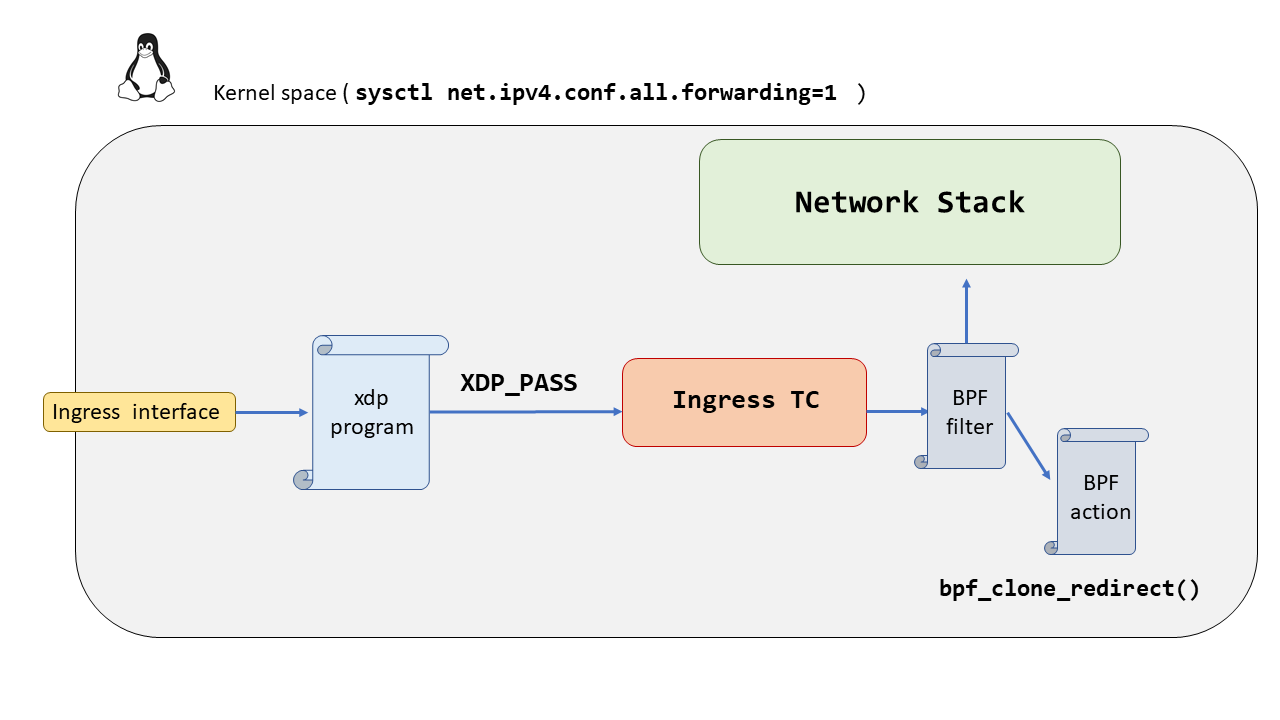
\includegraphics[width=16cm]{archivos/img/dev/xdp/case05/scenario_04.png}
    \caption{Solución propuesta para el Case05 - XDP}
    \label{fig:case05_xdp_ether_scenario3}
\end{figure}

De esta forma, en el \gls{tc} ya se tendría el manejo de la estructura \texttt{sk\_buff} y por ende, ya se podría hacer uso del \textit{helper} \gls{bpf} para clonar el paquete y hacer un reenvío a cada una de las interfaces que se quiera, para completar así el broadcast.


\vspace{1cm}
\textbf{Compilación}\\
\par

Para compilar el programa \gls{xdp} se ha dejado un Makefile preparado en este directorio al igual que en el case04 (\ref{xdp_ether_case04}), por lo que para compilarlo únicamente hay que seguir las indicaciones del bloque \ref{code:case04_xdp_ether_compilacion}.

\begin{lstlisting}[language= bash, style=Consola, caption={Compilación programa XDP - Case05},label=code:case05_xdp_ether_compilacion]
    # En caso de no haber entrado en el directorio asignado del caso de uso
    cd TFG/src/use_cases/xdp/case05
    
    
    # Hacemos uso del Makefile suministrado 
    sudo make
\end{lstlisting}
\vspace{0.5cm}

Si tiene dudas sobre el proceso de compilación del programa \gls{xdp} le recomendamos que vuelva al case02 (\ref{xdp_ether_case02}) donde se hace referencia al \textit{flow} dispuesto para la compilación de los programas \gls{xdp}.


\vspace{1cm}
\textbf{Puesta en marcha del escenario}\\
\par

Para comprobar el funcionamiento de los programas \gls{xdp} se hará uso de las \textit{Network Namespaces} (más información en la sección \ref{namespaces}). Como ya se comentaba, para que no suponga una barrera de entrada el concepto de las \textit{Network Namespaces}, se ha dejado escrito un script para levantar el escenario, y para su posterior limpieza. Es importante señalar que el script debe ser lanzado con permisos de root. Para levantar el escenario debemos ejecutar dicho script como se indica en el bloque \ref{code:case03_xdp_ether_escenario}.\\
\par
Para limpiar la máquina del escenario recreado anteriormente, se puede correr el mismo script indicándole ahora el parámetro \texttt{-c} (\textit{Clean}). En el peor de los casos, y si se cree que la limpieza se no se ha realizado de manera satisfactoria, se puede llevar a cabo un reinicio de la máquina consiguiendo así que todos los entes no persistentes (\gls{veth}, netns..) desaparezcan del equipo.

\begin{lstlisting}[language= bash, style=Consola, caption={Puesta en marcha del escenario - Case05},label=code:case05_xdp_ether_escenario]
    # Para levantar el escenario (Importante hacerlo con permisos de super usuario)
    sudo ./runenv.sh -i
    
    
    # Una vez finalizado la comprobación del caso de uso, limpiaremos nuestra maquina:
    sudo ./runenv.sh -c
\end{lstlisting}
\vspace{0.5cm}
Una vez levantado el escenario, tendríamos el escenario que se muestra en la figura \ref{fig:case05_xdp_ether_scenario4} montado con tres \textit{Network Namespaces} y pares de \gls{veth}s para interconectarlas. Los programas irán anclados a las interfaces de la \textit{Network Namespace} \texttt{switch}.
% figura escenario
\begin{figure}[ht]
    \centering
    \includegraphics[width=16cm]{archivos/img/dev/xdp/case05/scenario_03.png}
    \caption{Escenario del Case05 - XDP}
    \label{fig:case05_xdp_ether_scenario4}
\end{figure}

\vspace{1cm}
\textbf{Carga del programa XDP}\\
\par
Una vez compilado tanto el programa \gls{xdp} como los programas \gls{bpf} que irán al \gls{tc}, es hora de cargarlos. Por lo que, para hacerlo y por mayor comodidad se abrirá un proceso de bash en la \textit{Network Namespace} switch. Acto seguido, se cargará el programa \gls{xdp}, y se incluirán los programas \gls{bpf} añadiendo una nueva qdisc con un filtro \gls{bpf} asociado que derivará en una acción. Dicha acción, será otro programa \gls{bpf} con la función de clonar los paquetes y mandarlos a otras interfaces.\\
\par
\begin{lstlisting}[language= bash, style=Consola, caption={Carga del programa XDP - Case05},label=code:case05_xdp_ether_load]
    # Nos abrimos un proceso de bash sobre la Network Namespace "switch"
    sudo ip netns exec switch bash
    
    # Cargamos el programa XDP_PASS
    sudo ./xdp_loader -d switch xdp_pass
    
    # Creamos la nueva qdisc
    sudo tc qdisc add dev switch ingress handle ffff:
    
    # Aplicamos a la qdisc creada un filtro BPF que en caso de matchear aplicará una acción (Otro programa BPF que hará nuestro broadcast)
    sudo tc filter add dev switch parent ffff: bpf obj bpf.o sec classifier flowid ffff:1 action bpf obj bpf.o sec action 
\end{lstlisting}

\vspace{1cm}
\textbf{Comprobación del funcionamiento}\\
\par
Para comprobar el funcionamiento del sistema de broadcast se realizará la siguiente prueba, donde desde la \textit{Network Namespace} por defecto se generarán ARP-Request hacia la IP de una de las \gls{veth}s de las \textit{Network Namespace} destino. \\
\par

Si el sistema de broadcast funciona correctamente, escuchando en las \textit{Network Namespace} destino \texttt{uno} y \texttt{dos}, se debería ver como los paquetes ARP-Request llegan sin problemas. Solo el ``Host" al cual iban dirigidos los ARP-Request será el que intentará contestarlos sin éxito al haber implementado un sistema unidireccional. Para solucionar esta limitación se propone hacer uso de los programas \gls{xdp} desarrollados en case04 (\ref{xdp_ether_case04}) para conseguir una comunicación bidireccional.\\
\par
\begin{lstlisting}[language= bash, style=Consola, caption={Comprobación del funcionamiento - Case05},label=code:case05_xdp_ether_func]
    # Generamos el ARP-REQUEST
    arping 10.0.0.2/3
    
    # Escuchamos en las Network Namespace destino a la espera de ver ARP-REQUEST.
    sudo ip netns exec uno tcpduml -l
    sudo ip netns exec dos tcpduml -l
\end{lstlisting}
\vspace{0.5cm}

En este caso no se podrá hacer uso del programa xdp\_stats para ver si realmente los programas \gls{xdp} están funcionando como se quiere que funcionen, ya que la lógica de broadcast se encuentra en el programa \gls{bpf} anclado como acción en un filtro del \gls{tc}.\\
\par
Como se puede apreciar en la figura \ref{fig:case05_xdp_ether_func}, los ARP-Request \fcolorbox{black}{green}{\rule{0pt}{2.5pt}\rule{2.5pt}{0pt}}\hspace{1mm} llegan a ambos Host, y solo aquel al cual iba dirigida la resolución ARP contesta. Pero como ya se comentaba antes, al no haber implementado un sistema de forwarding, la comunicación únicamente está planteada en un sentido.\\
\par
Esta funcionalidad se podría aumentar haciendo uso de los programas desarrollados en el caso de uso anterior (\ref{xdp_ether_case04}). Por lo que se concluye afirmando que se ha podido hacer broadcast, pero no de forma exclusiva con \gls{xdp} ya que se ha tenido que añadir \gls{bpf} nativo en el \gls{tc}.

% figura escenario
\begin{figure}[ht]
    \centering
    \includegraphics[width=16cm]{archivos/img/dev/xdp/case05/demo_case05_edited.png}
    \caption{Comprobación de funcionamiento del Case05 - XDP}
    \label{fig:case05_xdp_ether_func}
\end{figure}
\newpage


%%%%%%%%%%%%%%%%%%%%%%%%%%%%%%%%%%%%%%%%%%%%%%%%%%%%%%%%%%%%%%%%%%%%%%%%%%%%%%%%%%%%%%%%%%%%%%%

\section{Casos de uso P4 en medios cableados}

En esta sección se introducirán todos los casos de uso realizados con la tecnología P4 en entornos cableados. Todos los casos de uso se han nombrado siguiendo la misma sintaxis que en el repositorio del \gls{tfg}, alojado en GitHub. Para \textbf{la instalación de las dependencias} de la tecnología P4, se ha generado el Anexo \ref{deps} donde se detallan todos los pasos a seguir. Se advierte al lector que quiera replicar los casos de uso, que  debe ser extremadamente cuidadoso con las dependencias del entorno P4 que instala, ya que, de querer hacer un \textit{upgrade} alguna de ellas puede generar numerosas incompatibilidades. \\
\par

Los casos de uso P4, al igual que con los casos de uso \gls{xdp}, se han dividido en partes diferenciadas con la finalidad de que la lectura de estos sea más clara y ordenada.

\begin{itemize}
    \item \textbf{Introducción}: En esta parte se abordarán las explicaciones teóricas complementarias, explicaciones propias sobre el caso de uso y comentarios sobre el código P4 desarrollado.
    
    \item \textbf{Compilación y puesta en marcha del escenario}: En esta parte se explicará al lector cómo proceder para compilar el programa P4 y cómo levantar el escenario. En este caso ambos procesos están integrados en un mismo Makefile, por lo que, la replicación los casos de uso será más amena.
    
    \item \textbf{Evaluación del funcionamiento}: Por último, se hará una evaluación sobre el funcionamiento del caso de uso empleando la CLI de Mininet.
\end{itemize}

Para que el lector pueda seguir el desarrollo de los casos de uso P4, a continuación se indica la tabla \ref{tab:P4_ether_usecases}, la cual expone en qué ruta del repositorio del \gls{tfg} se puede encontrar dicho caso de uso, y un vídeo demostración donde el autor va comentando paso a paso el caso de uso y su evaluación. \\
\par
\vspace{0.2cm}
\begin{table}[ht]
\centering
\resizebox{\textwidth}{!}{%
\begin{tabular}{|l|c|c|}
\hline
\rowcolor[HTML]{EFEFEF} 
\multicolumn{1}{|c|}{\cellcolor[HTML]{EFEFEF}\textbf{Caso de uso}} & \textbf{Enlace al repositorio} & \textbf{Enlace al vídeo demostración  } \\ \hline
case01 - Drop                                                      & \href{https://github.com/davidcawork/TFG/tree/master/src/use_cases/p4/case01}{\texttt{Enlace al código}}                         & \href{https://youtu.be/RKdi6SC5jYQ}{Enlace al vídeo}                                \\ \hline
case02 - Pass                                                      & \href{https://github.com/davidcawork/TFG/tree/master/src/use_cases/p4/case02}{\texttt{Enlace al código}}                         & \href{https://youtu.be/5X78simgC60}{Enlace al vídeo}                                \\ \hline
case03 - Echo server                                               & \href{https://github.com/davidcawork/TFG/tree/master/src/use_cases/p4/case03}{\texttt{Enlace al código}}                          & \href{https://youtu.be/H8R6T_W34gM}{Enlace al vídeo}                                \\ \hline
case04 - Layer 3 forwarding                                        & \href{https://github.com/davidcawork/TFG/tree/master/src/use_cases/p4/case04}{\texttt{Enlace al código}}                           & \href{https://youtu.be/La-_JCXut1Y}{Enlace al vídeo}                                \\ \hline
case05 - Broadcast                                                 & \href{https://github.com/davidcawork/TFG/tree/master/src/use_cases/p4/case05}{\texttt{Enlace al código}}                          & \href{https://youtu.be/jExo0mj8t6k}{Enlace al vídeo}                                \\ \hline
\end{tabular}
}
\caption{Resumen de la documentación sobre los casos de uso P4 en entornos cableados}
\label{tab:P4_ether_usecases}
\end{table}
\vspace{0.5cm}
En esta ocasión, como ya se comentaba en el capitulo de Análisis y Diseño (\ref{analisisPreimplementacion}), la plataforma que se utilizará para evaluar el funcionamiento de los programas P4 en entornos cableados será Mininet. Por lo que si usted no está familiarizado con la herramienta Mininet, se le recomienda que acuda a la sección \ref{mininet} donde se hace una introducción a esta herramienta.

\newpage

%%%%%%%%%%%%%%%%%%%%%%%%%%%%%%%%%%%%%%%%%%%%%%%%%%%%%%%%%%%%%%%%%%%%%%%%%%%%%%%%%%%%%%%%
%   Casos de uso P4 medio Cableados
\subsection{Case01 - Drop}
\label{p4_ether_case01}
En este caso de uso se probará que es posible descartar todos los paquetes recibidos con un programa P4. Como tal, el programa P4 no es suficiente para probar esta funcionalidad, ya que requiere de una plataforma que sea capaz de soportar el lenguaje P4. Según se comentó en el capítulo de Análisis y Diseño (Cap. \ref{analisisPreimplementacion}), se hará uso de soft-switch llamado behavioral-model, \gls{bmv2} en adelante, para testear los programas P4 y de Mininet como escenario para recrear las topologías de Red. \\
\par

Antes de continuar con el caso de uso, se quiere remarcar un detalle importante. Continuamente se estará refiriendo al \gls{bmv2} como un ``switch", pero se debe entender que con el lenguaje P4 estamos definiendo el \textit{datapath} que tendrá la entidad que cargue con el programa P4, en este caso el  \gls{bmv2}. Por lo que, la denominación de switch puede no ser totalmente correcta, ya que depende del programa P4 que porte para comportarse como un switch. Nótese que el uso del término ``switch" deriva de la denominación de dispositivos programables en entornos SDN, que tradicionalmente se nombraron como ``switches" \\
\par

Debido a esto, el \gls{bmv2} puede actuar como un hub, un switch, un router o un firewall, etc. Dependerá de la funcionalidad implementada en el programa P4. Se aprovechará la interfaz implementada del \gls{bmv2} con Mininet, desarrollada desde la equipo de p4Lang, para conseguir integrar estos nodos en el escenario de red pudiendo así comprobar el funcionamiento del programa P4 desarrollado.\\
\par

\vspace{0.2cm}
\textbf{Compilación y puesta en marcha del escenario}\\
\par

Para la compilación del programa P4 se hará uso del compilador p4c. Este es el compilador de referencia para el lenguaje P4, es modular y permite escoger distintos \textit{targets} para llevar a cabo la compilación. El proceso de compilación de los programas P4 se lleva a cabo en dos etapas, una etapa de compilación de \textit{frontend} donde se genera un archivo \texttt{*.p4info}, el cual recoge todos los atributos necesarios del programa P4 en tiempo de ejecución ( identificadores de tablas, su estructura, \textit{actions}.. ), y una etapa de \textit{backend}, en la cual se hace uso del archivo generado \texttt{*.p4info} para generar los archivos necesarios para programar al \textit{target} en cuestión.\\
\par

% figura escenario
\begin{figure}[ht]
    \centering
    \includegraphics[width=5cm]{archivos/img/dev/p4/case01/compilation_bmv2.png}
    \caption{Proceso de compilación programa P4}
    \label{fig:case01_p4_ether_intro}
\end{figure}

Por ejemplo, el compilador de \textit{backend} que ataca al BMV2 genera un fichero \texttt{*.json}. Este fichero será suficiente para establecer todo el \textit{datapath} según lo programado en el programa P4. El target del compilador p4c que se utilizará es el \texttt{p4c-bm2-ss}, P4 simple\_switch - bmv2, el cual soporta la arquitectura \textbf{v1model}.\\
\par
Con la finalidad de poner en marcha del escenario, se ha dejado escrito un Makefile, el cual compilará el programa P4, generando los ficheros \texttt{*.p4info} y \texttt{*.json}. Acto seguido, se lanzará el script llamado \texttt{run\_exercise.py}, el cual levantará toda la topología descrita en el fichero \texttt{scenario/topology.json} con Mininet. Cada ``switch" de la topología tendrá implementada toda la lógica descrita en el programa P4 dentro de una instancia del \gls{bmv2}. A continuación, en la figura \ref{fig:case01_p4_ether_intro2} se puede ver una imagen resumen del levantamiento de un único ``switch".\\
\par
\vspace{0.5cm}
% figura escenario
\begin{figure}[ht]
    \centering
    \includegraphics[width=15cm]{archivos/img/dev/p4/case01/setup.png}
    \caption{Proceso puesta en marcha de un switch BMv2 \cite{p42}}
    \label{fig:case01_p4_ether_intro2}
\end{figure}

\vspace{0.5cm}

Debido a que las personas que quieran replicar los casos de uso puede que no estén muy familiarizadas con todo este proceso de compilación y carga en los procesos de \gls{bmv2}, se ha dispuesto un de un Makefile para automatizar las tareas de compilación y carga de los programas, y también, para las tareas de limpieza del caso de uso una vez finalizada su demostración. Entonces, para proceder con la puesta en marcha del caso de uso, se deben seguir los pasos indicados en el bloque \ref{code:case01_p4_ether_load}.

\newpage

\begin{lstlisting}[language= bash, style=Consola, caption={Compilación programa P4 y puesta en marcha del escenario  - Case01},label=code:case01_p4_ether_load]
    # Entramos al directorio 
    cd TFG/src/use_cases/p4/case01

    # Hacemos uso del Makefile
    sudo make run
\end{lstlisting}
\vspace{0.5cm}

% figura escenario
\begin{figure}[ht]
    \centering
    \includegraphics[width=16cm]{archivos/img/dev/p4/case01/scenario.png}
    \caption{Escenario del Case01 - P4}
    \label{fig:case01_p4_ether_scenario}
\end{figure}

Una vez se haya finalizado la comprobación del funcionamiento del caso de uso, se debe hacer uso de otro target (\textit{clean}) del Makefile para limpieza total del directorio.

\begin{lstlisting}[language= bash, style=Consola, caption={Limpieza del escenario P4 - Case01},label=code:case01_p4_ether_unload]
    # Hacemos uso del Makefile
    sudo make clean
\end{lstlisting}
\vspace{0.5cm}
Es importante señalar que este target limpiará tanto los ficheros auxiliares para la carga del programa P4 en el \gls{bmv2}, como los directorios de \texttt{pcaps}, \texttt{log}, y \texttt{build} generados en la puesta en marcha del escenario. Por lo que, si se desea conservar las capturas de las distintas interfaces de los distintos \gls{bmv2}, se deben copiar o limpiar del escenario a mano siguiendo las indicaciones del bloque \ref{code:case01_p4_ether_unload2}.

\begin{lstlisting}[language= bash, style=Consola, caption={Limpieza segura del escenario P4 - Case01},label=code:case01_p4_ether_unload2]
    # Limpiamos Mininet
    sudo mn -c
    
    # Limpiamos los directorios generados dinámicamente en la carga del escenario
    sudo rm -rf build logs
\end{lstlisting}


\vspace{0.5cm}
\textbf{Comprobación del funcionamiento}\\
\par

Una vez realizado el \texttt{make run} en este directorio, se tendrá levantada la topología descrita para este caso de uso, la cual se puede apreciar en la figura \ref{fig:case01_p4_ether_scenario}. La topología de este caso de uso se compondrá de una instancia del \gls{bmv2} (\texttt{s1}), y de dos host (\texttt{h1}, \texttt{h2}) que se conectarán al ``switch". Como ya se comentaba anteriormente, la topología puede encontrarse descrita bajo el directorio \texttt{scenario}, en un fichero JSON llamado \texttt{topology.json}. En este fichero también se describe la localización de los archivos que describen el plano de control de cada ``switch" de la topología. En todos los casos de uso, se ha respetado los nombres tipo utilizados por la organización de p4Lang, \texttt{sX-runtime.json}, donde X es el número que ocupa dicho switch en la topología de Mininet. Volviendo de nuevo a la comprobación del funcionamiento del caso de uso, se tendrá la CLI de Mininet abierta, por lo que se abrirá una terminal para el \texttt{host1} y otra para el \texttt{host2}.

\begin{lstlisting}[language= bash, style=Consola, caption={Comprobación de funcionamiento - Case01},label=code:case01_p4_ether_func]
    mininet>  xterm h1 h2
\end{lstlisting}
\vspace{0.5cm}

Ahora con ambas terminales abiertas, desde el \texttt{h2} se pondrá a escuchar por su interfaz. Se puede utilizar wireshark, o el sniffer que el lector crea conveniente. En este caso por simplicidad y no disponer de una interfaz gráfica, se utilizará tcpdump (\ref{tcpdump}).

% figura escenario
\begin{figure}[ht]
    \centering
    \includegraphics[width=9cm]{archivos/img/dev/p4/case01/demo_case01_1_edited.png}
    \caption{Comprobación de funcionamiento (Ping) del Case01 - P4}
    \label{fig:case01_p4_ether_func1}
\end{figure}
\newpage
\begin{figure}[ht]
    \centering
    \includegraphics[width=11cm]{archivos/img/dev/p4/case01/demo_case01_2_edited.png}
    \caption{Comprobación de funcionamiento (Sniffer) del Case01 - P4}
    \label{fig:case01_p4_ether_func2}
\end{figure}


Una vez que se esté escuchando en la interfaz del \texttt{host2}, se hará ping \fcolorbox{black}{ProcessBlue}{\rule{0pt}{2.5pt}\rule{2.5pt}{0pt}}\hspace{1mm} desde el \texttt{host1} al \texttt{host2} y no se debería tener conectividad. Como se puede ver en las figuras \ref{fig:case01_p4_ether_func1} y \ref{fig:case01_p4_ether_func2}, el programa P4 desarrollado funciona correctamente. Para asegurarse de que realmente se está ejecutando el action para tirar paquetes se puede consultar los logs del \gls{bmv2}, los cuales generan un fichero de log por cada instancia target del simple switch que se haya levantado. \\
\par
Estos logs se encuentran en el directorio \texttt{logs}, y cada fichero de log pertenece a un único ``switch", llevando el mismo nombre que este en Mininet. En este caso, si se quisieran monitorizar los logs del \texttt{s1} bastaría con seguir las indicaciones del bloque \ref{code:case01_p4_ether_func2}.

\begin{lstlisting}[language= bash, style=Consola, caption={Comprobación de funcionamiento - Case01},label=code:case01_p4_ether_func2]
    # Entramos al directorio 
    cd TFG/src/use_cases/p4/case01

    # Monitorizamos los logs del Switch (s1) 
    tail -f logs/s1.log
\end{lstlisting}
\subsection{Case02 - Pass}
\label{P4_ether_case02}

Como se puede apreciar en esta sección, no se ha desarrollado ningún programa P4. Esto se debe a que no hay equivalente en P4 del código de retorno \texttt{XDP\_PASS}, por ello, no se puede hacer nada en este caso de uso. A continuación, se indica el porqué no se encuentra un equivalente entre ambas tecnologías. El código de de retorno en \gls{xdp} es una forma para llevar a cabo una acción con el paquete que llega a la interfaz, en la cual hay anclado un programa \gls{xdp}. Para más información sobre los códigos de retorno consultar la sección \ref{TecnologiaXDP} donde se indica en detalle cuantos hay, para qué sirven y qué limitaciones tienen.\\
\par

En este caso, el código de retorno \texttt{XDP\_PASS} implica que el paquete se pasa al siguiente punto del procesamiento del \textit{stack} de red en el Kernel de Linux. Es decir, si el programa está anclado a la \gls{nic}, se dejará pasar el paquete al \gls{tc}, de ahí al propio \textit{stack} de red para parsear sus cabeceras, y más adelante, pasárselo a la interfaz de sockets. En P4, el entorno donde se llevarán a cabo los casos de uso será Mininet con ``switches" (\gls{bmv2}) y host. Los ``switches" (\gls{bmv2}) es un soft-switch que permite inyectarle código P4, con el cual se puede definir el \textit{datapath} del mismo.\\
\par

Ahora bien, aquí viene la gran diferencia entre ambas tecnologías, con \gls{xdp} siempre se puede pasar el paquete al Kernel para que se encargue el del procesamiento, pero en P4, se debe definir de forma exclusiva todo el \textit{datapath}, por lo que no hay a quién delegar el paquete, dado que se tiene que encargar el propio programa P4. Entonces, como tal, no habría equivalente del \texttt{XDP\_PASS} en P4.
\subsection{Case03 - Echo server}
\label{P4_ether_case03}


En este caso de uso desarrollaremos un servidor de Echo que responda todos los pings que le lleguen. Como tal el programa P4 no es suficiente para probar esta funcionalidad, como ya se mencionó, se requiere de una plataforma que sea capaz de soportar el lenguaje P4, el \gls{bmv2}. \\
\par

El programa P4 deberá ser capaz de analizar los paquetes que le lleguen, analizarlos y filtrarlos. Solo aquellos paquetes filtrados serán los que se deberán responder. ¿Cómo se filtrarán? Se añadirán nuevos estados en el parser que comprueben si las cabeceras ICMP están presentes. Por ello, antes de nada se debe declarar las cabeceras ICMP necesarias para poder así analizar las cabeceras de los paquetes que lleguen.

\begin{lstlisting}[language=C, style=P4-color, caption={Estructura cabecera ICMP - Case03},label=code:case03_p4_ether_prog1]
    header icmp_t {
    	bit<8> type;
    	bit<8> code;
    	bit<16> checksum;
    }
\end{lstlisting}
\vspace{0.5cm}

Como se quería que este programa P4 fuera compatible con direccionamiento IPv6 se han añadido también los equivalentes en ICMPv6 y la cabecera de red de IPv6, ver bloque \ref{code:case03_p4_ether_prog2}.

\begin{lstlisting}[language=C, style=P4-color, caption={Estructura cabeceras IPv6 e ICMPv6  - Case03},label=code:case03_p4_ether_prog2]
    header ipv6_t {
       bit<4> version;
       bit<8> trafficClass;
       bit<20> flowLabel;
       bit<16> payloadLen;
       bit<8> nextHdr;
       bit<8> hopLimit;
       ip6Addr_t srcAddr;
       ip6Addr_t dstAddr;	
    }
    
    
    header icmp6_t {
       bit<8> type;
       bit<8> code;
       bit<16> checksum;
    }
\end{lstlisting}
\vspace{0.5cm}

Ahora que ya se tiene las cabeceras definidas, se deberá preocuparse en definir las macros asociadas a los posibles \textit{ethertypes} que se quieran manejar, IPv4 y IPv6. De forma adicional, se deberán definir los códigos de protocolo de las cabeceras de red, para asegurare que sobre la cabecera de red únicamente se procesarán aquellos paquetes que porten información ICMP. Se tuvo que consultar la RFC asociada a IPv6 para saber que codificación hacían con el campo de \textit{nextHeader} y por lo visto utilizan los mismo valores que en IPv4. A continuación, en la figura \ref{code:case03_p4_ether_prog3} se puede ver la definición de dichas macros y el extracto de la RFC asociada a la codificación de las cabeceras IPv6 .\\
\par

\begin{lstlisting}[language=C, style=P4-color, caption={Macros para parsear L2 y L3  - Case03},label=code:case03_p4_ether_prog3]
    /*	---	Layer 2 MACROS	     ---	*/
    const bit<16> ETHERTYPE_IPV4 = 0x0800;
    const bit<16> ETHERTYPE_IPV6 = 0x86dd;
    
    /*	---	Layer 3 MACROS	     ---	*/
    const bit<8> IP_PROTOCOL_ICMP = 0x01;
    const bit<8> IP_PROTOCOL_ICMPv6 = 0x3a; 
    const bit<8> ICMP_ECHO_REQUEST_TYPE = 0x08;
    const bit<8> ICMP_ECHO_REQUEST_CODE = 0x00;
    const bit<8> ICMP_ECHO_REPLY_TYPE = 0x00;
    const bit<8> ICMP_ECHO_REPLY_CODE = 0x00;
    
    /*
    *   According to RFC 2460, the codes of the protocol immediately above,
    *   layer 4, are the same as those used in IPv4. And I quote:
    *
    *   Next Header          8-bit selector.  Identifies the type of header
    *                       immediately following the IPv6 header.  Uses the
    *                       same values as the IPv4 Protocol field [RFC-1700
    *                       et seq.].
    *
    */
\end{lstlisting}
\vspace{0.5cm}

Como se ha indicado en el bloque \ref{code:case03_p4_ether_prog3},  de forma adicional se han definido macros sobre los valores con los que se va estar trabajando (\texttt{ECHO-Request} y \texttt{ECHO-Reply}). De esta forma el código resultante de las \textit{actions} será más interpretable y sostenible. Teniendo ya todas las herramientas necesarias para declarar los nuevos estados del parser, se puede proceder con el siguiente bloque del datapath.\\
\par

Una vez que se es capaz de filtrar los paquetes que interesan, se va a ver cómo se ha implementado la lógica de procesamiento de aquellos paquetes que ya han sido filtrados. Es de interés interceptar todos los paquetes ICMP que lleguen a nuestro ``switch" para así contestarlos desde el mismo "switch". Por ello, se hará uso del bit de validez de las cabeceras que han sido analizadas correctamente, es decir, si el paquete contiene dichas cabeceras. De no contenerlas, su bit de validez estará a \textit{false}. A continuación en la figura \ref{code:case03_P4_ether_prog4}, mostramos la lógica de control del bloque \textit{Ingress}.


\begin{lstlisting}[language=C, style=P4-color, caption={Lógica para filtrar paquetes ICMP e ICMPv6  - Case03},label=code:case03_P4_ether_prog4]
    /*  
     *  De esta forma nos aseguramos que unicamente procesamos paquetes ICMP,
     *  o en su defecto ICMPv6.
     *
     */
    
    
    apply {
    	if(hdr.ipv4.isValid() && hdr.icmp.isValid()){
    	        echo();
    	}else if (hdr.ipv6.isValid() && hdr.icmp6.isValid()){
    		echo6();
    	}
    }
\end{lstlisting}
\vspace{0.5cm}

Ya se tienen todos los paquetes ICMP filtrados, solo quedaría programar la lógica para modificar las cabeceras de dicho paquete para conseguir contestar satisfactoriamente al emisor del ping. Para ello, se hará uso de un \textit{action}, una función. El cual intercambiará tanto MAC destino-origen, como IP destino-origen, modificará la cabecera ICMP para indicarle que se trata de un \textit{reply}, y por último mandará el paquete por el puerto por el cual llegó al \gls{bmv2}, de esta forma se asegura que dicho paquete llegará al emisor del mismo.\\
\par


\begin{lstlisting}[language=C, style=P4-color, caption={Lógica para procesar paquetes ICMP  - Case03},label=code:case03_p4_ether_prog5]
    action echo (){
    	/*	---	Auxiliary variables	---	*/
        macAddr_t temp_mac = hdr.ethernet.srcAddr;
        ip4Addr_t temp_ip = hdr.ipv4.srcAddr;
    
    	/*      ---     Swap MACs     ---     */
    	hdr.ethernet.srcAddr = hdr.ethernet.dstAddr;
        hdr.ethernet.dstAddr = temp_mac;
    
    	/*      ---     Swap Ips     ---     */
     	hdr.ipv4.srcAddr = hdr.ipv4.dstAddr;
    	hdr.ipv4.dstAddr = temp_ip;
      
    	/*      ---     Re-Write ICMP's type and code     ---     */
    	hdr.icmp.type = ICMP_ECHO_REPLY_TYPE;
    	hdr.icmp.code = ICMP_ECHO_REPLY_CODE;
    
    	/*      ---     Forward the packet to the ingress intf     ---     */
    	standard_metadata.egress_spec = standard_metadata.ingress_port;

    }  
\end{lstlisting}
\vspace{0.5cm}

\newpage

Préstese atención a la última sentencia de la función donde le indicamos que saque el paquete por la misma interfaz por la cual ha entrado. Este es el equivalente directo al código de retorno en \gls{xdp}, \texttt{XDP\_TX} con el cual re-circulábamos el paquete de la misma forma a la interfaz de entrada.\\
\par

Como curiosidad, es interesante comentar que el campo \textit{checksum} de la cabecera ICMP debe ser re-calculado de nuevo por lo que se deberá hacer antes del \textit{Egress}. Esto supuso un problema, ya que continuamente estaban saliendo paquetes con un \textit{checksum} incorrecto,  lo cual se comprobó con el disector de Wireshark. Finalmente se vio que no había que incluir el campo \textit{checksum} en la nueva suma del nuevo \textit{checksum}\footnote{Habría sido genial que la RFC asociada hubiera estado más clara al respecto.}, de esta forma los paquetes \texttt{ECHO-Reply} que salían ya llevaban el \textit{checksum} calculado correctamente.\\
\par


\vspace{1cm}
\textbf{Compilación y puesta en marcha del escenario}\\
\par

Para la compilación del programa P4 se hará uso de nuevo del compilador P4c (más información sobre el proceso de compilación en la subsección \ref{p4_ether_case01}).\\
\par

Dado que las personas que quieran replicar los casos de uso puede que no estén muy familiarizadas con todo este proceso de compilación y carga en los procesos de \gls{bmv2}, se ha dispuesto un de un Makefile para automatizar las tareas de compilación y carga, y las tareas de limpieza del caso de uso. Para la puesta en marcha del caso de uso se deben seguir los pasos indicados en el bloque \ref{code:case03_p4_ether_load}.\\
\par

\begin{lstlisting}[language= bash, style=Consola, caption={Compilación programa P4 y puesta en marcha del escenario - Case03},label=code:case03_p4_ether_load]
    # Entramos al directorio 
    cd TFG/src/use_cases/p4/case03

    # Hacemos uso del Makefile
    sudo make run
\end{lstlisting}
\vspace{0.5cm}

Una vez se haya finalizado la comprobación del funcionamiento del caso de uso, se debe hacer uso de otro target (\textit{clean}) del Makefile para limpieza total del directorio según se indica en el bloque \ref{code:case03_p4_ether_unload}.

\begin{lstlisting}[language= bash, style=Consola, caption={Limpieza del escenario P4 - Case03},label=code:case03_p4_ether_unload]
    # Hacemos uso del Makefile
    sudo make clean
\end{lstlisting}
\vspace{0.5cm}

Es importante señalar que este target limpiará tanto los ficheros auxiliares para la carga del programa P4 en el \gls{bmv2}, como los directorios de \texttt{pcaps}, \texttt{log}, y \texttt{build} generados en la puesta en marcha del escenario. Por lo que si se desea conservar las capturas de las distintas interfaces de los distintos \gls{bmv2}, se deben copiar o limpiar del escenario a mano siguiendo las indicaciones del bloque \ref{code:case03_p4_ether_unload2}.\\
\par

\begin{lstlisting}[language= bash, style=Consola, caption={Limpieza segura del escenario P4 - Case03},label=code:case03_p4_ether_unload2]
    # Limpiamos Mininet
    sudo mn -c
    
    # Limpiamos los directorios generados dinámicamente en la carga del escenario
    sudo rm -rf build logs
\end{lstlisting}


\vspace{1cm}
\textbf{Comprobación del funcionamiento}\\
\par

Una vez realizado el make run en este directorio, se tendrá levantada la topología descrita para este caso de uso, la cual se puede apreciar en la figura \ref{fig:case03_p4_ether_scenario}. Como en el \textit{datapath} no se contempla el manejo del protocolo ARP, se ha añadido el ARP entry a directamente en los hosts, desde el fichero \texttt{topology.json} consiguiendo así que no se genere la resolución ARP en el envío de los \texttt{ECHO-Request}. En este caso, la demostración se va hacer uso de IPv4, en el caso de querer hacerla con IPv6, se deberá añadir la entrada analoga para el protocolo ND  (\textit{Neighbor Discovery}).\\
\par
% figura escenario
\begin{figure}[ht]
    \centering
    \includegraphics[width=16cm]{archivos/img/dev/p4/case03/scenario.png}
    \caption{Escenario del Case03 - P4}
    \label{fig:case03_p4_ether_scenario}
\end{figure}

Volviendo de nuevo a la comprobación del funcionamiento del caso de uso, se tendrá la CLI de Mininet abierta, por lo que se procederá a abrir una terminal para el \texttt{host1}, desde el cual se llevará a cabo los pings.

\begin{lstlisting}[language= bash, style=Consola, caption={Comprobación de funcionamiento - Case03},label=code:case03_p4_ether_func]
    mininet>  xterm h1
\end{lstlisting}
\vspace{0.5cm}

Una vez que se tenga la terminal abierta, se procederá a abrir Wireshark. En este caso se recomineda Wireshark ya que se podrá filtrar y comprobar de una forma más sencilla la validez de los \textit{checksums}.

% figura escenario
\begin{figure}[ht]
    \centering
    \includegraphics[width=15.5cm]{archivos/img/dev/p4/case03/demo_case03_edited.png}
    \caption{Comprobación de funcionamiento del Case03 - P4}
    \label{fig:case03_p4_ether_func1}
\end{figure}

Como se puede ver en la figura \ref{fig:case03_p4_ether_func1}, todo funciona correctamente ya que se están recibiendo respuesta a los pings \fcolorbox{black}{green}{\rule{0pt}{2.5pt}\rule{2.5pt}{0pt}}\hspace{1mm}. De forma adicional, se puede comprobar con Wireshark como el \textit{checksum} de la cabecera ICMP viene correctamente calculado.


\subsection{Case04 - Layer 3 forwarding}
\label{P4_ether_case04}

En este caso de uso, se abordará la implementación un forwarding a nivel de red, capa 3, por lo que el hipotético ``switch" será ahora un un router muy básico y con muy pocas funcionalidades. Por ello conviene recordar las anotaciones que se hicieron sobre el \gls{bmv2} y por qué no debemos definirlo únicamente como un soft-switch, ya que depende del programa P4 que porte para definir su \textit{datapath} y su interfaz con el plano de control.\\
\par

La motivación de este caso de uso, es ver el equivalente en P4 que tiene el código de retorno \gls{xdp} llamado \texttt{XDP\_REDIRECT}. En el anterior caso de uso ya se hacía uso de la información de metadatos para elegir el puerto de salida del paquete. Por lo que podríamos afirmar que este es el equivalente directo al forwarding en \gls{xdp}, solo que aquí en P4 resulta más sencillo ya que únicamente indicamos por número de puerto mientras que \gls{xdp} se debía obtener el \textit{ifindex} de la interfaz a la cual íbamos a hacer el reenvío. Como se puede apreciar en la figura \ref{code:case04_p4_ether_prog1}, unicamente le indicamos el puerto por el cual debe salir el paquete.\\
\par

\begin{lstlisting}[language=C, style=P4-color, caption={Redirección del paquete - Case04},label=code:case04_p4_ether_prog1]
    standard_metadata.egress_spec = port
\end{lstlisting}
\vspace{0.5cm}

Pero, ¿Qué son los números de puerto? ¿Cuando se han establecido estos identificadores? Estos números de puerto se establecen cuando se levanta la instancia del \gls{bmv2}. Se asocia interfaz real con un número identificativo. Serán estos números identificativos los números de puerto de cada ``switch". De esta manera el ``switch" tiene a su alcance todos sus posibles puertos. El levantamiento de las instancias de \gls{bmv2} se llevan a cabo con la carga del script \texttt{run\_exercise.py}. Este a su vez hace uso de la clase \texttt{P4RuntimeSwitch} definida en la interfaz de Python hacia Mininet,  para levantar dicho ``switch" pasándole los parámetros adecuados. Se puede levantar una instancia del \gls{bmv2} siguiendo las indicaciones del bloque \ref{code:case04_p4_ether_instacia}.\\
\par

\begin{lstlisting}[language= bash, style=Consola, caption={Ejecución de instancia del BMv2 - Case04},label=code:case04_p4_ether_instacia]
    sudo simple_switch_grpc --log-console --dump-packet-data 64 \
                        –i 0@veth0 -i 1@veth2 … [--pcap] --no-p4 \
                        --grpc-server-addr 0.0.0.0:50051 --cpu-port 255 \
                        test.json
\end{lstlisting}
\vspace{0.5cm}
Una vez entendido de dónde salen los números de puerto, se debe plantear la siguiente cuestión, ¿Cómo un programa P4 es capaz de conocer los posibles puertos de los que puede disponer para reenviar un paquete?\\
\par
No puede, y tampoco es lógico que en un programa P4, donde se define el \textit{datapath}, ya estén preestablecidos los números de puerto posibles a manejar. Ya que si eso fuera así, se tendría que tener distintos programas P4 por cada entidad con un número de puertos distintos (únicamente para implementar un único \textit{datapath}). No es viable. Por ello, toda la información relativa a los puertos, asociada al forwarding, generalmente suele venir desde el plano de control quien tiene constancia de los puertos de dicho ``switch".\\
\par

Por ejemplo, si se quiere hacer forwarding de un paquete a un puerto en especifico dado su IP, necesitaremos que el plano de control indique el criterio a seguir, qué IPs están asociadas a según que puertos. Esta interfaz entre el plano de datos y el plano de control esta definidas por tablas.\\
\par

Desde el programa P4 se tiene que definir el esqueleto de la tabla, indicando qué \textit{actions}
están disponibles, qué parámetros reciben esas \textit{actions}, qué criterio de match tendrá la tabla, sobre qué \textit{keys} se realizará el \textit{lookup} y cuál es el número máximo de entradas en dicha tabla. A continuación, se muestra la figura \ref{fig:case03_p4_ether_tablas} que resume bastante bien la funcionalidad de las tablas.\\
\par

% figura escenario
\begin{figure}[ht]
    \centering
    \includegraphics[width=16cm]{archivos/img/dev/p4/case04/table.png}
    \caption{Funcionamiento de las tablas en P4 \cite{p42}}
    \label{fig:case03_p4_ether_tablas}
\end{figure}
\vspace{0.2cm}

Por tanto, desde el plano de control, bien vía P4Runtime ó vía json con los ficheros \texttt{sX-runtime.json} (que se cargarán a través de la CLI-\gls{bmv2}), se rellenarán las entradas de dicha tabla y los parámetros de las acciones a llevar a cabo cuando haya un \textit{hit} con dicha entrada. En este caso se asociarán IPs a una acción de forwarding donde  se le  suministrará por qué puerto tiene que salir el paquete y que MAC destino debe llevar.\\
\par

Una vez entendidos los números de puerto y el concepto de las tablas, se debe abordar el cómo hacer una acción de forwarding para reenviar los paquetes que lleguen al \gls{bmv2}. Esta acción de forwarding deberá se capaz de actualizar el puerto de salida, actualizar la MAC destino y decrementar en uno el campo \texttt{ttl} de la cabecera IP. A continuación, se indica la acción propuesta para llevar a cabo dicho cometido (Ver bloque \ref{code:case04_p4_ether_prog1}).

\begin{lstlisting}[language=C, style=P4-color, caption={Acción propuesta para llevar a cabo el forwarding - Case04},label=code:case04_p4_ether_prog2]
    /*
     * Se quiso hacer uso del operador '-=' pero la sintaxis de P4 no lo permite :(
     */
    
    action ipv4_forward(macAddr_t dstAddr, egressSpec_t port) {
            standard_metadata.egress_spec = port;
            hdr.ethernet.srcAddr = hdr.ethernet.dstAddr;
            hdr.ethernet.dstAddr = dstAddr;
            hdr.ipv4.ttl = hdr.ipv4.ttl - 1;
    }
\end{lstlisting}
\vspace{0.5cm}
Teniendo la acción ya disponible, solo quedaría aplicar la tabla en nuestra pipeline del programa P4 y ya se estaría haciendo un forwarding en capa 3.

\vspace{0.5cm}
\textbf{Compilación y puesta en marcha del escenario}\\
\par

Para la compilación del programa P4 se hará uso del compilador P4c (más información sobre el proceso de compilación en la subsección \ref{p4_ether_case01}).\\
\par

Dado que las personas que quieran replicar los casos de uso puede que no estén muy familiarizadas con todo este proceso de compilación y carga en los procesos de \gls{bmv2}, se ha dispuesto un de un Makefile para automatizar las tareas de compilación y carga, y las tareas de limpieza del caso de uso. Entonces para la puesta en marcha del caso de uso se deben seguir los pasos indicados en el bloque \ref{code:case04_p4_ether_load}.

\begin{lstlisting}[language= bash, style=Consola, caption={Compilación programa P4 y puesta en marcha del escenario - Case04},label=code:case04_p4_ether_load]
    # Entramos al directorio 
    cd TFG/src/use_cases/p4/case04

    # Hacemos uso del Makefile
    sudo make run
\end{lstlisting}
\vspace{0.5cm}

Una vez se haya finalizado la comprobación del funcionamiento del caso de uso, se debe hacer uso de otro target (\textit{clean}) del Makefile para limpieza total del directorio según se indica en el bloque \ref{code:case04_p4_ether_unload}.

\begin{lstlisting}[language= bash, style=Consola, caption={Limpieza del escenario P4 - Case04},label=code:case04_p4_ether_unload]
    # Hacemos uso del Makefile
    sudo make clean
\end{lstlisting}
\vspace{0.5cm}

Es importante señalar que este target limpiará tanto los ficheros auxiliares para la carga del programa P4 en el \gls{bmv2}, como los directorios de \texttt{pcaps}, \texttt{log}, y \texttt{build} generados en la puesta en marcha del escenario. Por lo que si se desea conservar las capturas de las distintas interfaces de los distintos \gls{bmv2}, cópielas o haga la limpieza del escenario a mano siguiendo las indicaciones del bloque \ref{code:case04_p4_ether_unload2}.
\begin{lstlisting}[language= bash, style=Consola, caption={Limpieza segura del escenario P4 - Case04},label=code:case04_p4_ether_unload2]
    # Limpiamos Mininet
    sudo mn -c
    
    # Limpiamos los directorios generados dinámicamente en la carga del escenario
    sudo rm -rf build logs
\end{lstlisting}


\vspace{0.5cm}
\textbf{Comprobación del funcionamiento}\\
\par


Así pues, después de realizar el \texttt{make run} en este directorio, se tendrá levantada la topología descrita para este caso de uso, la cual se puede apreciar en la figura \ref{fig:case04_p4_ether_scenario}. Como en el \textit{datapath} no se contempla el manejo de ARP, se ha añadido el ARP entry a directamente desde el fichero \texttt{topology.json} consiguiendo así que no se genere la resolución ARP en el envío de los \texttt{ECHO-Request}. Este arreglo es poco elegante ya que se le está indicando un hipotético \textit{gateway} que no existe, y se está añadiendo un ARP entry con la MAC de dicho \textit{gateway}. De esta forma, todos los paquetes saldrán con la MAC destino indicada en la entry y no se producirá la resolución ARP. Al llegar al ``switch" el paquete verá modificada su MAC destino en función de su IP destino, por lo que la ``chapuza" no irá a más.\\
\par

% figura escenario
\begin{figure}[ht]
    \centering
    \includegraphics[width=12cm]{archivos/img/dev/p4/case04/scenario.png}
    \caption{Escenario del Case04 - P4}
    \label{fig:case04_p4_ether_scenario}
\end{figure}


Volviendo de nuevo a la comprobación del funcionamiento del caso de uso, se tendrá la CLI de Mininet abierta, por lo que simplemente se probará la conectividad entre todos los hosts. Esto se puede realizar ejecutando la orden \texttt{pingall}, la cual ejecutará pings entre todos los hosts, comprobando así la conectividad bidireccional de todos los \textit{paths} preestablecidos en el escenario. De forma adicional, se podría hacer uso de un \textit{sniffer} para comprobar que los paquetes llegan con el campo \texttt{ttl} modificado, en función de los saltos que ha dado el paquete. Según se puede apreciar en la figura \ref{fig:case04_p4_ether_func}, hay perfecta conectividad entre todos los hosts de la topología.

\newpage

% figura escenario
\begin{figure}[ht]
    \centering
    \includegraphics[width=12cm]{archivos/img/dev/p4/case04/demo_case04_edited.png}
    \caption{Comprobación de funcionamiento del Case04 - P4}
    \label{fig:case04_p4_ether_func}
\end{figure}

\newpage


\subsection{Case05 - Broadcast}
\label{P4_ether_case05}

En este caso de uso, se desarrollará un programa p4 que haga Broadcast. En este caso únicamente se hará Broadcast a nivel de enlace, capa 2. La motivación de este caso de uso es ver la diferencia de dificultad respecto del entorno \gls{xdp} donde se tuvo que anclar de manera adicional un \textit{bytecode} e\gls{bpf} en el \gls{tc}, además del propio programa \gls{xdp} anclado en la interfaz para lograr realizar un broadcast.\\
\par

Para conseguir hacer una difusión de los paquetes en P4, se hará uso de los llamados grupos multicast. Los grupos multicast se utilizan para difundir por una serie de números de puertos del ``switch". Para más información sobre de dónde salen estos números de puerto vuelva al case04 (\ref{P4_ether_case04}) donde se explica que representan estos identificadores y cuándo se asignan. Cada grupo multicast tiene un identificador único, y en él se definen una serie de réplicas, es decir, cuántas copias del paquete se llevarán a cabo y qué números de puerto se verán afectados.\\
\par

Los grupos multicast se definen en la información del plano de control del ``switch", bien vía P4Runtime ó vía json con los ficheros \texttt{sX-runtime.json}. A continuación, en el bloque \ref{code:case05_p4_ether_json} se deja la definición del grupo multicast utilizado para este caso de uso.  

\begin{lstlisting}[language= bash, style=Consola, caption={Ejemplo Json Grupo Multicast - Case05},label=code:case05_p4_ether_json]
    "multicast_group_entries" : [
        {
          "multicast_group_id" : 1,
          "replicas" : [
            {
              "egress_port" : 1,
              "instance" : 1
            },
            {
              "egress_port" : 2,
              "instance" : 1
            },
            {
              "egress_port" : 3,
              "instance" : 1
            }
          ]
        }
      ]
\end{lstlisting}
\vspace{0.5cm}

Con esta definición se está indicando que todos los paquetes que pertenezcan al grupo multicast cuyo identificador sea 1, generarán una copia del paquete por los puertos del ``switch" 1, 2 y 3. Es decir por todos los puertos de nuestro ``switch" para este caso de uso. Por tanto la acción de broadcast/multicast será la siguiente:

\begin{lstlisting}[language=C, style=P4-color, caption={Acción propuesta para llevar a cabo el Broadcast - Case05},label=code:case05_p4_ether_prog1]
    action multicast() {
            standard_metadata.mcast_grp = 1;
    }
\end{lstlisting}
\vspace{0.5cm}

Únicamente se asigna el paquete a dicho grupo multicast, y el \gls{bmv2} ya se encarga de clonar el paquete y reenviarlo por los puertos indicados. Dado que no se quiere generar paquetes por el puerto por el cual se recibió el paquete de broadcast, podría plantearse tener tantos grupos multicast como puertos tuviera el \gls{bmv2}, generando copias por puertos específicos y asociando cada grupo multicast a los paquetes que llegaran por cada puerto. Pero esta solución no sería del todo escalable. Por ello, como se puede ver en el grupo multicast (bloque de código \ref{code:case05_p4_ether_json}), se generan copias en todos los puertos asociados a esta instancia del \gls{bmv2}. Será por tanto en la fase de egress cuando se comprueben los metadatos del paquete, y si el puerto de entrada es igual al puerto de salida, se descartará el paquete (Ver bloque de código \ref{code:case05_p4_ether_prog2}).\\
\par

\begin{lstlisting}[language=C, style=P4-color, caption={Acción propuesta para descartar paquetes sobrantes de Broadcast - Case05},label=code:case05_p4_ether_prog2]
    control MyEgress(inout headers hdr,
                 inout metadata meta,
                 inout standard_metadata_t standard_metadata) {
    
        action drop() {
            mark_to_drop(standard_metadata);
        }
    
        apply {
            // Prune multicast packet to ingress port to preventing loop
            if (standard_metadata.egress_port == standard_metadata.ingress_port)
                drop();
        }
}

\end{lstlisting}
\vspace{0.5cm}

En este caso, se ha encontrado que implementar esta funcionalidad en P4 es mucho más sencillo que con \gls{xdp}. Por lo que, en caso de necesitar probar protocolos que implementen la difusión como parte de su lógica, es mucho más recomendable y viable hacer uso de P4.

\vspace{0.5cm}
\textbf{Compilación y puesta en marcha del escenario}\\
\par

Para la compilación del programa P4 se hará uso del compilador P4c (más información sobre el proceso de compilación en la subsección \ref{p4_ether_case01}).\\
\par

Dado que las personas que quieran replicar los casos de uso puede que no estén muy familiarizadas con todo este proceso de compilación y carga en los procesos de \gls{bmv2}, se ha dispuesto un de un Makefile para automatizar las tareas de compilación y carga, y las tareas de limpieza del caso de uso. Entonces para la puesta en marcha del caso de uso se deben seguir los pasos indicados en el bloque \ref{code:case05_p4_ether_load}.

\begin{lstlisting}[language= bash, style=Consola, caption={Compilación programa P4 y puesta en marcha del escenario - Case05},label=code:case05_p4_ether_load]
    # Entramos al directorio 
    cd TFG/src/use_cases/p4/case05

    # Hacemos uso del Makefile
    sudo make run
\end{lstlisting}
\vspace{0.5cm}

Una vez se haya finalizado la comprobación del funcionamiento del caso de uso, se debe hacer uso de otro target (\textit{clean}) del Makefile para limpieza total del directorio según se indica en el bloque \ref{code:case05_p4_ether_unload}.

\begin{lstlisting}[language= bash, style=Consola, caption={Limpieza del escenario P4 - Case05},label=code:case05_p4_ether_unload]
    # Hacemos uso del Makefile
    sudo make clean
\end{lstlisting}
\vspace{0.5cm}

Es importante señalar que este target limpiará tanto los ficheros auxiliares para la carga del programa P4 en el \gls{bmv2}, como los directorios de \texttt{pcaps}, \texttt{log}, y \texttt{build} generados en la puesta en marcha del escenario. Por lo que si se desea conservar las capturas de las distintas interfaces de los distintos \gls{bmv2}, cópielas o haga la limpieza del escenario a mano siguiendo las indicaciones del bloque \ref{code:case05_p4_ether_unload2}.\\
\par

\begin{lstlisting}[language= bash, style=Consola, caption={Limpieza segura del escenario P4 - Case04},label=code:case05_p4_ether_unload2]
    # Limpiamos Mininet
    sudo mn -c
    
    # Limpiamos los directorios generados dinámicamente en la carga del escenario
    sudo rm -rf build logs
\end{lstlisting}


\vspace{0.5cm}
\textbf{Comprobación del funcionamiento}\\
\par
Una vez realizado el make run en el directorio, se tendrá levantada la topología descrita para este caso de uso, la cual se puede apreciar en la figura \ref{fig:case05_p4_ether_scenario}.


% figura escenario
\begin{figure}[ht]
    \centering
    \includegraphics[width=16cm]{archivos/img/dev/p4/case05/scenario.png}
    \caption{Escenario del Case05 - P4}
    \label{fig:case05_p4_ether_scenario}
\end{figure}

Volviendo de nuevo a la comprobación del funcionamiento del caso de uso, se tendrá la CLI de Mininet abierta, por lo que se procederá a abrir tres terminales, una por cada host de la topología. Esto se puede hacer conseguir siguiendo las indicaciones del bloque \ref{code:case05_p4_ether_func1}.

\begin{lstlisting}[language= bash, style=Consola, caption={Apertura de terminales - Case05},label=code:case05_p4_ether_func1]
    mininet> xterm h1 h2 h3 
\end{lstlisting}
\vspace{0.5cm}

Cuando ya se tengan las tres terminales abiertas, se procederá a escuchar las interfaces de los \texttt{host2} y \texttt{host3} con la finalidad de comprobar si realmente los paquetes están siendo clonados por los puertos indicados por el grupo multicast. Se hará uso de la herramienta tcpdump, podríamos utilizar también Wireshark.

\begin{lstlisting}[language= bash, style=Consola, caption={Puesta en escucha - Case05},label=code:case05_p4_ether_func2]
    # Hacemos lo mismo en el host2 y host3
    tcpdump -l
\end{lstlisting}
\vspace{1cm}

Una vez que se tenga tcmdump escuchando desde el \texttt{host2} y \texttt{host3}, se va a generar ARP-Request desde el \texttt{host1} para que así, al ir con MAC destino en difusión se propague por todos los posibles puertos del ``switch" menos por aquel por el cual le llegó. Por tanto, para generar dicho ARP-Request se seguirán los pasos del bloque \ref{code:case05_p4_ether_func3}.

\begin{lstlisting}[language= bash, style=Consola, caption={Generación de ARP-Request - Case05},label=code:case05_p4_ether_func3]
    # Desde el host1
    arping 10.0.2.2
\end{lstlisting}
\vspace{1cm}

Como se puede apreciar en la figura \ref{fig:case05_p4_ether_func1}, el caso de uso funciona correctamente. Se puede observar cómo el paquete ARP-Request está llegando tanto al \texttt{host2} como al \texttt{host3}. Pero solo será el \texttt{host2}, en este caso, el que contesta ya que va dirigido a éste. Se puede ver que al \texttt{host3} solo le llega un ARP-Request, y después se detiene.\\
\par
Esto es así ya que al completarse la resolución ARP el \texttt{host1} ya conoce la dirección MAC del \texttt{host2}, por tanto los ARP-Request que se generen a posteriori llevarán la MAC destino la del \texttt{host2}, entonces el ``switch" no lo difundirá por todos su puertos, se lo pasará directamente al \texttt{host2}.\\
\par

\newpage

\begin{figure}[h!]
    \centering
    \begin{subfigure}[b]{\textwidth}
    	\centering
        \includegraphics[width=8.2cm]{archivos/img/dev/p4/case05/demo_case05_1_edited.png}
        \caption{Ejecución de arping en el Host1 hacia el Host2}
        \label{fig:case05_p4_ether_func_ping}
    \end{subfigure}
    \par\bigskip
    \begin{subfigure}[b]{\textwidth}
    	\centering
        \includegraphics[width=12cm]{archivos/img/dev/p4/case05/demo_case05_2_edited.png}
        \caption{Escucha con Tcpdump en el Host3}
        \label{fig:case05_p4_ether_func_list1}
    \end{subfigure}
    \par\bigskip
    \begin{subfigure}[b]{\textwidth}
    	\centering
        \includegraphics[width=12cm]{archivos/img/dev/p4/case05/demo_case05_3_edited.png}
        \caption{Escucha con Tcpdump en el Host2}
        \label{fig:case05_p4_ether_func_list2}
    \end{subfigure}
    
    \caption{Comprobación de funcionamiento del Case05 - P4}
    \label{fig:case05_p4_ether_func1}
\end{figure}

\newpage


%%%%%%%%%%%%%%%%%%%%%%%%%%%%%%%%%%%%%%%%%%%%%%%%%%%%%%%%%%%%%%%%%%%%%%%%%%%%%%%%%%%%%%%%

\section{Casos de uso P4 en medios inalámbricos}

En esta sección se introducirán todos los casos de uso realizados con la tecnología P4 en entornos inalámbricos. Todos ellos se han nombrado siguiendo la misma sintaxis que en el repositorio del \gls{tfg}, alojado en GitHub. Para \textbf{la instalación de las dependencias} de la tecnología P4, se ha dejado escrito el anexo \ref{deps} donde se detallan todos los pasos a seguir. De forma adicional, será necesario la instalación de Mininet-WiFi.\footnote{Más adelante se indicará que versión se debe instalar.} \\
\par

Estos casos de uso, al igual que los anteriores, se han dividido en partes diferenciadas con la finalidad de que la lectura de estos sea más clara y ordenada. Puesto que muchos conceptos/desarrollos serán iguales que en los casos de uso P4 en entornos cableados, se referenciará directamente al lector a las secciones correspondientes.

\begin{itemize}
    \item \textbf{Introducción}: En esta parte se abordará las explicaciones teóricas complementarias, explicaciones propias sobre el caso de uso y comentarios sobre el código P4 desarrollado.
    
    \item \textbf{Compilación}: En esta parte se explicará al lector cómo proceder para compilar el programa P4. 
    
    \item \textbf{Puesta en marcha del escenario}: En esta parte se explicará cómo levantar el escenario. 
    
    \item \textbf{Evaluación del funcionamiento}: Por último se hará una evaluación sobre el funcionamiento del caso de uso haciendo uso de la CLI de Mininet-WiFi.
\end{itemize}

Para que el lector pueda seguir el desarrollo de los casos de uso P4, a continuación se indica la tabla \ref{tab:P4_wifi_usecases}, la cual expone en qué ruta del repositorio del \gls{tfg} se puede encontrar dicho caso de uso, y un vídeo demostración donde el autor va comentando paso a paso el caso de uso y su evaluación. \\
\par

\begin{table}[ht]
\centering
\resizebox{\textwidth}{!}{%
\begin{tabular}{|l|c|c|}
\hline
\rowcolor[HTML]{EFEFEF} 
\multicolumn{1}{|c|}{\cellcolor[HTML]{EFEFEF}\textbf{Caso de uso}} & \textbf{Enlace al repositorio} & \textbf{Enlace al vídeo demostración  } \\ \hline
case01 - Drop                                                      & \href{https://github.com/davidcawork/TFG/tree/master/src/use_cases/p4-wireless/case01}{\texttt{Enlace al código}}                         & \href{https://youtu.be/7e3NQc4qQEo}{Enlace al vídeo}                                \\ \hline
case02 - Pass                                                      & \href{https://github.com/davidcawork/TFG/tree/master/src/use_cases/p4-wireless/case02}{\texttt{Enlace al código}}                         & \href{https://youtu.be/ZP1oaX3qiD4}{Enlace al vídeo}                                \\ \hline
case03 - Echo server                                               & \href{https://github.com/davidcawork/TFG/tree/master/src/use_cases/p4-wireless/case03}{\texttt{Enlace al código}}                          & \href{https://youtu.be/4C4yPG6MVkI}{Enlace al vídeo}                                \\ \hline
case04 - Layer 3 forwarding                                        & \href{https://github.com/davidcawork/TFG/tree/master/src/use_cases/p4-wireless/case04}{\texttt{Enlace al código}}                           & \href{https://youtu.be/w1mzL-I9Naw}{Enlace al vídeo}                                \\ \hline
case05 - Broadcast                                                 & \href{https://github.com/davidcawork/TFG/tree/master/src/use_cases/p4-wireless/case05}{\texttt{Enlace al código}}                          & \href{https://youtu.be/XU2djyzIyvU}{Enlace al vídeo}                                \\ \hline
\end{tabular}
}
\caption{Resumen de la documentación sobre los casos de uso P4 en entornos inalámbricos}
\label{tab:P4_wifi_usecases}
\end{table}
En esta ocasión, como ya se comentaba en el capitulo de Análisis y Diseño (\ref{analisisPreimplementacion}), la plataforma que se utilizará para evaluar el funcionamiento de los programas P4 en entornos cableados será Mininet-WiFi. Pero como se indicó, la plataforma no contempla ningún tipo de nodo que de soporte al \gls{bmv2}, por lo que será necesario desarrollar previamente una integración del \gls{bmv2} en Mininet-WiFi.


%%%%%%%%%%%%%%%%%%%%%%%%%%%%%%%%%%%%%%%%%%%%%%%%%%%%%%%%%%%%%%%%%%%%%%%%%%%%%%%%%%%%%%%%
%   Integración y Casos de uso P4 medio inalámbricos
\subsection{Integración del \glsentryshort{bmv2} en Mininet-WiFi}
\label{mn-wifi_bmv2_integration}

% Intro
En esta subsección se abordará la integración del \gls{bmv2} en Mininet-WiFi. La integración se ha dividido en tres partes. En las dos primeras se estudiará y analizará, conceptos básicos y desarrollos previos que serán de gran utilidad a la hora de abordar el desarrollo de la interfaz \gls{bmv2} en Mininet-WiFi.

\subsubsection{Análisis de la interfaz \glsentryshort{bmv2} - Mininet}

Desde el equipo de \textit{p4lang} se quiso suministrar un entorno de pruebas donde se pudiera probar los programas P4 desarrollados. El soft-switch donde iban a cargar el programa P4 ya lo tenían, que es el \gls{bmv2}, pero les faltaba una plataforma donde poder desplegar dicho ``switch" e interconectarlo con otras entidades de red. Esta plataforma sería Mininet, una herramienta de emulación de redes.\\
\par

Mininet generalmente se utiliza para emular entornos \gls{sdn} con switches y controladores. Por ello, para lograr la integración de su nuevo switch con los switches ya disponibles en Mininet, tuvieron que añadir una nueva clase llamada \texttt{P4Switch}. Esta nueva clase, heredaría de la clase \texttt{Switch} de Mininet, añadiendo así todos los métodos y atributos necesarios para la orquestación del \gls{bmv2}.\\
\par

Usualmente, cuando se trabaja con Mininet se desarrollan scripts donde se define la topología de la red a emular. En este caso, para brindar de una mayor facilidad a los usuarios de los tutoriales de P4\footnote{\url{https://github.com/p4lang/tutorials}}, las topologías se definen en archivos \texttt{*.json}, los cuales definen toda la topología de red y toda la información del plano de control de cada ``switch" P4. Un ejemplo de dicho archivo pueden encontrarse \href{https://github.com/davidcawork/TFG/blob/master/src/use_cases/p4/case01/scenario/topology.json}{\textbf{aquí}}. De este modo, se consigue abstraer el la definición de la topología del propio script de orquestación de la misma. El script de orquestación de la topología el cual hará uso de la API de Python de Mininet será el script \texttt{run\_exercise.py}, que se puede encontrar \href{https://github.com/davidcawork/TFG/blob/master/src/use_cases/p4/utils/run_exercise.py}{\textbf{aquí}}. De esta manera se tendrá tantos ficheros \texttt{*.json} como topologías se quieran, pero un único script de orquestación.\\
\par

El script \texttt{run\_exercise.py} inicializa un objeto de la clase \texttt{ExerciseRunner} el cual leerá el fichero \texttt{*.json}, procesará la topología con la ayuda de la clase \texttt{ExerciseTopo} y levantará la topología haciendo uso de la API de Python de Mininet. A continuación, en la figura \ref{fig:analysis_p4_wifi_1} se puede apreciar un diagrama UML donde se indica la relación de clases del entrypoint en el levantamiento de los distintos casos de uso.\\
\par

Como ya se comentaba anteriormente, para lograr la integración del \gls{bmv2} en Mininet se tuvo que crear la clase \texttt{P4Switch}. Esta nueva clase, heredaría de la clase \texttt{Switch} de Mininet. A su vez, se crearían nuevas clases hijas de la clase \texttt{P4Switch}, la más importante \texttt{P4RuntimeSwitch} la cual se utilizaría para configurar dicho ``switch" vía P4Runtime. Si se desea ver una vista más amplia de esta relación de clases, ir a la figura \ref{fig:analysis_p4_wifi_2}.

\newpage

% uml_1
% figura escenario
\begin{figure}[ht]
    \centering
    \includegraphics[width=13cm]{archivos/img/dev/p4-wifi/analysis/run_exercise_pertenencia.png}
    \caption{UML del punto de entrada de la interfaz BMv2 - Mininet}
    \label{fig:analysis_p4_wifi_1}
\end{figure}

%uml_2
% figura escenario
\begin{figure}[h!]
    \centering
    \includegraphics[width=13.5cm]{archivos/img/dev/p4-wifi/analysis/run_exercise_class_names_only.png}
    \caption{UML interfaz BMv2 - Mininet}
    \label{fig:analysis_p4_wifi_2}
\end{figure}



\subsubsection{Análisis del funcionamiento interno de Mininet-WiFi}

Una vez que se revisó el funcionamiento interno de la API de Mininet-P4, se da paso a analizar Mininet-WiFi en profuncidad. Como se comentaba en el capítulo \ref{estadoArte}, Mininet-WiFi es una herramienta de emulación de redes wireless que ha nacido de Mininet, es decir es un fork de este. Al ser un fork comparte gran parte de la jerarquía de clases así como su capacidad para simular ciertos elementos de la red. Aun así, si bien se ha mencionado en numerosas ocasiones que Mininet-WiFi esta desarrollado a partir de Mininet, la capacidad de emulación de interfaces \textit{Wireless} la toma de subsistema wireless de Linux.\\
\par

La arquitectura de virtualización empleada en Mininet-WiFi funciona de forma similar a la Mininet; se hace uso de la herramienta \texttt{mnexec}\footnote{\url{https://github.com/intrig-unicamp/mininet-wifi/blob/master/mnexec.c}} para lanzar distintos procesos de bash en nuevas \textit{Network Namespaces}, uno por cada nodo independiente de la red. De estos procesos colgarán todos los procesos relativos a los distintos nodos de la red. Cuando la emulación haya terminado, se matarán dichos procesos de bash, consiguiendo que no haya ninguna condición de referenciación de las \textit{Network Namespaces}, y estas sean eliminadas por el Kernel.\\
\par

De esta manera, los nodos de la red ya estarían aislados entre sí, por loque lo único que quedaría por virtualizar son las capacidades \textit{wireless} de los nodos que las requieran. Para ellos se hará uso del subsistema \textit{wireless}  del Kernel de Linux, más concretamente el módulo \texttt{mac80211\_hwsim} el cual creará las interfaces \textit{wireless}  en nuestro equipo. Este módulo se comunicará con framework \texttt{mac80211} el cual proveerá de las capacidades de gestión de acceso al medio de la interfaz \textit{wireless} . Además, en el espacio de Kernel aun hay un bloque más, llamado cfg80211, el cual servirá de API para la configuración de las cabeceras 802.11. Esta configuración puede ser realizada por la interfaz netlink de espacio de usuario llamada nl80211. Para la configuración de los puntos de acceso, se hará uso del programa \texttt{HostApd} el cual indicándole la configuración del punto de acceso y la interfaz sobre la cual debe correr, emulará el funcionamiento de un punto de acceso estándar. En la  figura \ref{fig:analysis_p4_wifi_3} se puede ver de manera resumida la arquitectura básica de Mininet-WiFi.\\
\par

% foto arch Mininet-wifis
% figura escenario
\begin{figure}[ht]
    \centering
    \includegraphics[width=15cm]{archivos/img/dev/p4-wifi/analysis/mininet_wifi_components.png}
    \caption{Arquitectura Mininet-WiFi \cite{7367387}}
    \label{fig:analysis_p4_wifi_3}
\end{figure}


En cuanto a la jerarquía de clases,únicamente cabe mencionar que es bastante similar a la de Mininet. Por destacar dos clases claves en la jerarquía de Mininet-WiFi, serían Node\_Wifi, de la cual heredan todos los nodos con capacidades wireless que posee Mininet-WiFi y por último, la clase IntfWireless, de la cual heredan todos los tipos de enlaces disponibles de Mininet-WiFi (Bajo el estándar \texttt{ieee80211}). A continuación,  en la figuras \ref{fig:analysis_p4_wifi_4} y \ref{fig:analysis_p4_wifi_5}, se indican los UML referentes a dichas clases.\\
\par

% uml_3 wifis
% figura escenario
\begin{figure}[ht]
    \centering
    \includegraphics[width=8cm]{archivos/img/dev/p4-wifi/analysis/uml_node.png}
    \caption{UML sobre las relaciones de las clases de tipo Nodo.}
    \label{fig:analysis_p4_wifi_4}
\end{figure}



Como se puede apreciar en los esquemas UML, se ha conseguido aislar la funcionalidad común en las clases padres, con la finalidad de optimizar la cantidad de código de las clases hijas. De esta forma, añadir nuevos tipos de enlaces y nodos en Mininet-WiFi resulta bastante asequible.\\
\par

% uml_4 wifis
% figura escenario
\begin{figure}[ht]
    \centering
    \includegraphics[width=15cm]{archivos/img/dev/p4-wifi/analysis/uml_link.png}
    \caption{UML sobre las relaciones de las clases de tipo Interfaz.}
    \label{fig:analysis_p4_wifi_5}
\end{figure}



\vspace{1cm}
\textbf{Linux Wireless Subsystem}\\
\par

El subsistema \textit{wireless} de Linux consiste en un set de varios módulos que se encuentran en el Kernel de Linux. Estos manejan la configuración del hardware bajo el estándar \texttt{ieee80211}, además de la gestión de la transmisión y la escucha de los paquetes de datos. Yendo de desde abajo hacia arriba en la arquitectura del subsistema, el primer bloque que se encuentra es el módulo mac80211\_hwsim. Este módulo como ya se comentaba es el responsable de crear las interfaces \textit{wireless} virtuales en Mininet-WiFi.\\
\par

% arch LWS
% figura escenario
\begin{figure}[ht]
    \centering
    \includegraphics[width=14cm]{archivos/img/dev/p4-wifi/analysis/linux_wireless_subsystem.JPG}
    \caption{Arquitectura del subsistema Wireless de Linux \cite{8330098}}
    \label{fig:analysis_p4_wifi_6}
\end{figure}

El objetivo principal de este módulo mac80211\_hwsim es facilitar a los desarrolladores de drivers de tarjetas \textit{wireless} la prueba de su código e interacción con el siguiente bloque llamado mac80211. Las interfaces virtualizadas no tienen ciertas limitaciones, es decir, a diferencia del hardware real, resulta más sencillo la creación de distintas pruebas con distintas configuraciones sin estar cohibidos por falta de recursos materiales. Este módulo generalmente recibe un único parámetro, que es el número de ``radios", interfaces virtuales, a virtualizar. Dado que las posibilidades que ofrece este módulo eran un poco reducidas, muchos \textit{wrappers} (``envoltorios al software original") han sido creados para ofrecer más funcionalidad a parte de la dada por el propio módulo. La mayoría de herramientas creadas hacen uso de la librería Netlink para comunicarse directamente con el subsistema en el Kernel y así conseguir configuraciones extra, como pueden ser añadir un \gls{rssi} o darle nombre a la interfaz. Un ejemplo de dichas herramientas sería la herramienta \texttt{mac80211\_hwsim\_mgmt}, la cual es usada por Mininet-WiFi para gestionar la creación de las interfaces \textit{wireless} en cada nodo que las requiera.\\
\par

Es importante mencionar el cambio de paradigma que existe en el subsistema \textit{wireless} de Linux con el concepto de interfaz. Generalmente se está acostumbrado a pensar en el concepto de interfaz como un elemento que gestiona el acceso al medio, capa dos, y el propio hardware, capa física, un ejemplo de ello sería una interfaz de Ethernet. Bien, pues en el subsistema wireless se desglosa la interfaz en dos capas \cite{8330098}. Una de ellas es la capa física (\textit{PHY}) donde se puede gestionar por ejemplo en que canal está escuchando la tarjeta wireless emulada. La otra capa es el acceso al medio, representado por las interfaces virtuales que ``cuelgan" de una tarjeta wireless.\\
\par
 La idea detrás de este paradigma, es que puede tener \textit{N} interfaces virtuales asociadas a la misma tarjeta WiFi emulada, lo que resultó sorprendente es que las interfaces virtuales funcionan principalmente con Ethernet (dejando de lado las que están en modo monitor).

\vspace{0.5cm}
\textbf{Limitaciones encontradas}\\
\par
\label{limitacionesEncontradas}

Como ya se ha comentado, la mayoría de interfaces virtuales asociadas a una tarjeta wireless emulada son del tipo de Ethernet, por lo que todos los paquetes que llegan vienen con cabeceras Ethernet. Esto supone una limitación ya que en los casos de uso se quería gestionar las cabeceras WiFi, pero si todas las interfaces virtuales son generalmente del de tipo Ethernet, no será posible.

% foto downstream
% figura escenario
\begin{figure}[ht]
    \centering
    \includegraphics[width=4cm]{archivos/img/dev/p4-wifi/analysis/linux_wireless_subsystem_tx.png}
    \caption{Flujo para la transmisión con el módulo mac80211\_hwsim \cite{5415877}}
    \label{fig:analysis_p4_wifi_7}
\end{figure}

Pero, ¿Qué sentido tiene tener convertir las cabeceras WiFi a cabeceras Ethernet? De momento la única razón que se ha encontrado de esta decisión de diseño, es hacer un diseño más sencillo de todos los drivers que operan bajo el módulo mac80211\_hwsim, que convierten a Ethernet y se lo entregan al stack de red para que lo gestione como un paquete más de una red cableada. De esta forma, las aplicaciones que operen a nivel de interfaz serán más extrapolables. 

% foto upstream
% figura escenario
\begin{figure}[ht]
    \centering
    \includegraphics[width=5cm]{archivos/img/dev/p4-wifi/analysis/linux_wireless_subsystem_rx.png}
    \caption{Flujo para la recepción con el módulo mac80211\_hwsim \cite{5415877}}
    \label{fig:analysis_p4_wifi_8}
\end{figure}

Pero, hay que mencionar que esto supone un gasto de recursos considerable, ya que el paquete es encolado hasta tres veces (driver, ethernet queue, qdisc queue) y se tiene que invertir tiempo y recursos en el proceso de traducción de las cabeceras.  \href{https://elixir.bootlin.com/linux/latest/C/ident/__ieee80211_data_to_8023}{\textbf{Aquí}}\footnote{\url{https://elixir.bootlin.com/linux/latest/C/ident/__ieee80211_data_to_8023}} se puede ver la función en el kernel donde se lleva a cabo ese proceso.\\
\par

Esto sucede generalmente y no siempre ya que en el único modo que una interfaz puede llegar a escuchar los paquetes WiFi es en el modo monitor. Pero el modo monitor está pensado únicamente para escuchar paquetes, no para transmitir. Este modo puede ser llevado al limite haciendo una inyección de paquetes (packet injection) por la interfaz.\\
\par

De esta forma se conseguiría el objetivo de manejar las cabeceras WiFi, pero dadas las competencias del \gls{tfg}, este desarrollo se escapa completamente. Ni si quiera Mininet-WiFi, siendo la herramienta de facto para emular redes \textit{wireless}, contempla el manejo de cabeceras WiFi. Por ello, este objetivo se plantea como un desarrollo a posteriori y se mencionará en el trabajo futuro (Ver sección \ref{trabajoFuturo}). \\
\par
El desarrollo pues sobre Mininet-WiFi, consistirá en la integración del \gls{bmv2} en Mininet-WiFi, y probar los casos de uso desarrollados para P4, bajo Mininet-WiFi. Las cabeceras que llegarán a la pipeline serán las de Ethernet, pero como ya se ha explicado, es el propio Kernel quien se encarga de hacer un \textit{casting} de las cabeceras WiFi hacia cabeceras Ethernet.\\
\par

\subsubsection{Desarrollo de la interfaz BMV2 - Mininet-WiFi}

Ahora que ya se tiene una idea sobre el funcionamiento interno de ambas herramientas, vamos a proceder a su integración. A la par que se estaba trabajando en el desarrollo de la integración del \gls{bmv2} en Mininet-WiFi, el investigador Ramon Fontes (desarrollador de la herramienta) abrió un Issue (es decir, una publicación de debate y ampliación de funcionalidad de GitHub) donde se exponía la intención de crear dicha integración. En este issue se pudo debatir con Ramon Fontes cómo debía hacerse dicho desarrollo.\\
\par

En concreto, se decidió hacer un jerarquía de clases genérica para el \gls{bmv2} para que de estas se puedan crear clases personalizadas con añadidos nuevos. Por así decirlo, estas clases serán la base para clases que controlen el \gls{bmv2} de una forma más particular.\\
\par
Una clase \texttt{P4AP}, la cual contiene todos los atributos y métodos comunes al \gls{bmv2} como son el path de ejecución del \gls{bmv2}, el json compilado del programa P4, el thrift-port, configuración de log y identificador básico del \gls{bmv2}. De esta clase se quiere que herede una clase llamada \texttt{P4RuntimeAP}, la cual proporcionará todos los elementos necesarios para dar soporte a la configuración vía P4Runtime vía gRPC-port del \gls{bmv2}.\\
\par

% Foto uml propio
% figura escenario
\begin{figure}[ht]
    \centering
    \includegraphics[width=15.5cm]{archivos/img/dev/p4-wifi/analysis/p4_Mininet_Wifi_UML.png}
    \caption{UML de la integración BMv2 - Mininet-WiFi}
    \label{fig:analysis_p4_wifi_9}
\end{figure}

Además debatiendo con Ramon Fontes sobre la implementación de estas clases,  indicó que sería de gran utilidad que dichas clases tuvieran soporte de ejecución en Network Namespaces, por lo que de forma paralela se tuvo que crear una clase llamada \texttt{Netns\_mgmt}\footnote{\url{https://github.com/davidcawork/TFG/tree/master/src/netns_mgmt}}. Esta clase ayudará a gestionar la ejecución de código Python en \textit{runtime} en una Network namespace indicada haciendo uso de la llamada al sistema \textbf{setns} la cual asocia el procesos sobre la cual se realiza esta llamada, a una \textit{Namespace} indicada.\\
\par

Con la ayuda de esta clase, \texttt{Netns\_mgmt}, se pudo conseguir configurar cada \gls{bmv2} en su propia \textit{Network Namespace}, por lo que la integración se dio por terminada. Adicionalmente se añadieron dos ejemplos a Mininet-WiFi con la finalidad de ayudar a las personas que vayan hacer uso de clase. Dichos ejemplos pueden ser encontrados \href{https://github.com/davidcawork/mininet-wifi/tree/p4/examples/p4}{\textbf{aquí}}.\footnote{\url{https://github.com/davidcawork/mininet-wifi/tree/p4/examples/p4}}\\
\par
Todo este desarrollo se llevo a cabo en un fork de Mininet-WiFi, y dentro de este en una rama en particular, en la cual se llevan a cabo todos los desarrollos de P4. Una vez finalizada la integración, se ofreció el desarrollo al repositorio oficial de Mininet-WiFi vía pull-request. Actualmente se ha dejado a la espera de hacer un \textit{upgrade} a las dependencias donde fue llevada a cabo la integración, ya que Mininet-WiFi está trabajando con las últimas versiones. En cambio, para el desarrollo de los casos de uso P4-wireless, se hará uso de las últimas versiones  estables de las dependencias del entorno P4.

\vspace{1cm}
\textbf{Puesta en marcha del Mininet-WiFi modificado}\\
\par
\label{mn_wifi_own_deps}

Para poder probar el desarrollo llevado a cabo con Mininet-WiFi se deberán seguir los pasos indicados en el bloque \ref{code:wifi_bmv2_integration_deps} previamente. Se deberá bajar el repositorio del fork de Mininet-WiFi. Se hará un checkout para moverse desde la rama master del repositorio a la rama de desarrollo de elementos P4.

\begin{lstlisting}[language= bash, style=Consola, caption={Instalación de Mininet-WiFi modificado},label=code:wifi_bmv2_integration_deps]
    # Se descarga el repositorio
    git clone https://github.com/davidcawork/mininet-wifi
    
    # Se adquieren las etiquetas y se cambia de rama
    cd mininet-wifi && git fetch
    git checkout p4
    
    # Se "recompilará" Mininet-Wifi
    sudo make install
\end{lstlisting}
\vspace{0.5cm}

Como la rama de desarrollo añade módulos nuevos a Mininet-WiFi se deberá ``recompilar" de nuevo haciendo un make install desde el directorio \texttt{/mininet-wifi}. Para que los módulos añadidos funcionen correctamente se deberán tener las dependencias del entorno P4, en la tabla \ref{tab:mn-wifi_bmv2_integration_deps} se pueden comprobar que versiones son requeridas.\\
\par

\begin{table}[ht]
\centering

\begin{tabular}{|c|c|}
\hline
\rowcolor[HTML]{EFEFEF} 
{\color[HTML]{24292E} \textbf{Dependencia}} & {\color[HTML]{24292E} \textbf{Versión requerida}} \\ \hline
\href{https://github.com/p4lang/behavioral-model}{\textbf{BMV2}}                                        & \texttt{b447ac4c0cfd83e5e72a3cc6120251c1e91128ab}          \\ \hline
\href{https://github.com/p4lang/PI}{\textbf{PI}}                                          & \texttt{41358da0ff32c94fa13179b9cee0ab597c9ccbcc}          \\ \hline
\href{https://github.com/p4lang/p4c}{\textbf{P4C}}                                         & \texttt{69e132d0d663e3408d740aaf8ed534ecefc88810}         \\ \hline
\href{https://github.com/protocolbuffers/protobuf}{\textbf{PROTOBUF}}                                    & \texttt{v3.2.0}                                        \\ \hline
\href{https://github.com/grpc}{\textbf{GRPC}}                                        & \texttt{v1.3.2}                                           \\ \hline
\end{tabular}%
\caption{Resumen de las versiones requeridas de la interfaz BMv2 - Mininet-WiFi}
\label{tab:mn-wifi_bmv2_integration_deps}
\end{table}


\subsection{Case01 - Drop}
\label{p4_wifi_case01}

En este caso de uso se probará que es posible descartar todos los paquetes recibidos con un programa P4 en una interfaz virtual \textit{Wireless}. Como tal el programa P4 no es suficiente para probar esta funcionalidad ya que requiere de una plataforma que sea capaz de soportar el lenguaje P4. Se hará uso de software switch llamado behavioral-model, \gls{bmv2} en adelante, para testear los programas P4, y de la integración desarrollada anteriormente con Mininet-WiFi como escenario para recrear las topologías de Red.\\
\par

Como este caso de uso ya se ha explicado anteriormente en el case01 de P4 cableado (Ver subsección \ref{p4_ether_case01}), y no hay ninguna diferencia inducida en el cambio de entorno según se explico en las sección anterior,  únicamente se harán indicaciones sobre como poder compilarlo y ejecutarlo. Importante, si usted está replicando este caso de uso, sin antes haber adecuado las dependencias necesarias de Mininet-WiFi con soporte del \gls{bmv2}, vuelva a este punto \ref{mn_wifi_own_deps} y siga los pasos indicados.

% figura escenario
\begin{figure}[ht]
    \centering
    \includegraphics[width=16cm]{archivos/img/dev/p4-wifi/case01/scenario.png}
    \caption{Escenario del Case01 - P4 Wireless}
    \label{fig:case01_p4_wifi_scenario}
\end{figure}

\vspace{0.2cm}
\textbf{Compilación}\\
\par

Para la compilación de este caso de uso, se ha dejado preparado un Makefile, por tanto no es necesario que el usuario aprenda a utilizar el compilador p4c. Si se quiere saber más sobre como funciona el proceso de compilación, qué etapas hay, como se le "inyecta" el \texttt{json} generado al \gls{bmv2}, o qué distintos \textit{targets} hay en función de la arquitectura, le recomendamos que vuelva al case01 (\ref{p4_ether_case01}). Para llevar a cabo la compilación solo se tendrá que seguir los pasos indicados en el bloque \ref{code:case01_p4_wifi_load}.

\begin{lstlisting}[language= bash, style=Consola, caption={Compilación programa P4  - Case01},label=code:case01_p4_wifi_load]
    # Entramos al directorio 
    cd TFG/src/use_cases/p4-wireless/case01

    # Hacemos uso del Makefile
    sudo make
\end{lstlisting}
\vspace{0.5cm}


Una vez ejecutado el make, se habrá generado una estructura de directorios que se utilizarán en el lanzamiento del caso de uso. Bajo el directorio \texttt{build} se podrá encontrar el \texttt{json} generado por el compilador, será este \texttt{json} quien tenga toda la información requerida para conformar el \gls{bmv2}.\\
\par

\vspace{0.2cm}
\textbf{Puesta en marcha del escenario}\\
\par

Al igual que en la compilación, se ha dejado preparado un script en Python para automatizar la puesta en marcha del escenario. Este script describe la topología que se utilizará en este caso de uso. Recordemos que es necesario volver hacer un \texttt{make install} para instalar los módulos adicionales generados para la integración del \gls{bmv2} y Mininet-WiFi, además de tener instaladas las versiones indicadas en el análisis de la integración. Estas dependencias se pueden encontrar en el apartado \ref{mn_wifi_own_deps} \\
\par

Una vez comprobado que posee todas la dependencias, simplemente se tendrá que ejecutar el script con el interprete de Python. Este script levantará la topología descrita en la figura \ref{fig:case01_p4_wifi_scenario}, compuesto por dos hosts y por una instancia del nodo \texttt{P4RuntimeAP}. El nodo \texttt{ap1}, del tipo \texttt{P4RuntimeAP}, tendrá dos interfaces, una wireless y un par de \gls{veth}.



\begin{lstlisting}[language= bash, style=Consola, caption={Puesta en marcha del escenario  - Case01},label=code:case01_p4_wifi_run]
    sudo python scenario.py
\end{lstlisting}
\vspace{0.2cm}


\vspace{0.5cm}
\textbf{Comprobación del funcionamiento}\\
\par

Tras las ejecución del script \texttt{scenario.py}, se tendría el escenario \ref{fig:case01_p4_wifi_scenario} levantado, y la CLI de Mininet-WiFi abierta. Para la comprobación de funcionamiento de este caso de uso, se van a seguir los mismos pasos que en el case01 (\ref{p4_ether_case01}) - P4 en un entorno alámbrico. Por tanto no se entrará en hacer explicaciones que se creen redundantes, se indicarán los pasos seguidos para llevar a cabo la comprobación de funcionamiento y los resultados de dichas pruebas. 

\begin{lstlisting}[language= bash, style=Consola, caption={Pasos a seguir para comprobar el funcionamiento - Case01},label=code:case01_p4_wifi_func1]
    mininet-wifi>  xterm sta1 h1
    
    # Se hará ping desde la estación Wifi al Host
    [sta1] ping 10.0.2.2
    
    
    # Se pondrá a escuchar en el Host
    [h1] tcpdump -l

\end{lstlisting}
\vspace{0.5cm}


% Figura
% figura escenario
\begin{figure}[ht]
    \centering
    \includegraphics[width=14cm]{archivos/img/dev/p4-wifi/case01/demo_case01_1_edited.png}
    \caption{Comprobación de funcionamiento (Ping) del Case01 - P4 Wireless}
    \label{fig:case01_p4_wifi_func1}
\end{figure}
\vspace{0.5cm}

Como se puede ver en la figura \ref{fig:case01_p4_wifi_func1}, no hay conectividad entre ambos nodos dado que el ping \fcolorbox{black}{green}{\rule{0pt}{2.5pt}\rule{2.5pt}{0pt}}\hspace{1mm} no está llegando. Por lo que, el programa P4 está funcionando según lo esperado, tirando los paquetes que llegan a su \textit{pipeline} de procesamiento. Para asegurarse de que realmente se está ejecutando el \textit{action} para tirar paquetes podemos consultar los logs del \gls{bmv2}, los cuales generan un fichero de log por cada instancia \textit{target} del \texttt{P4RuntimeAP} que se haya levantado.\\
\par

\newpage

\begin{figure}[ht]
    \centering
    \includegraphics[width=14cm]{archivos/img/dev/p4-wifi/case01/demo_case01_2_edited.png}
    \caption{Comprobación de funcionamiento (Sniffer) del Case01 - P4 Wireless}
    \label{fig:case01_p4_wifi_func2}
\end{figure}
\subsection{Case02 - Pass}
\label{p4_wifi_case02}


Como se puede apreciar, en este directorio no hay ningún programa P4, al igual que en caso de uso P4, case02 (\ref{P4_ether_case02}),  en entornos cableados. Esto se debe a que no hay equivalente en P4 del código de retorno \texttt{XDP\_PASS}, por ello, no se puede hacer nada en este caso de uso. El código de de retorno en \gls{xdp} es una forma para llevar a cabo una acción con el paquete que llega a la interfaz, en la cual hay anclado un programa \gls{xdp}. En este caso el código de retorno  \texttt{XDP\_PASS} implica que el paquete se pasa al siguiente punto del procesamiento del \textit{stack} de red en el Kernel de Linux. Es decir, si el programa está anclado a la \gls{nic}, se dejará pasar el paquete al \gls{tc}, de ahí al propio \textit{stack} de red para parsear sus cabeceras, y más adelante, dárselo de comer a la interfaz de sockets.\\
\par

En P4, el entorno donde se llevaran a cabo los casos de uso será Mininet-WiFi con \gls{ap}s (\gls{bmv2}) y host. Los \gls{ap}s (\gls{bmv2}) son un software switch en los que podemos inyectar código P4, con el cual podemos definir el \textit{datapath} del mismo.\\
\par

Ahora bien, aquí viene la gran diferencia entre ambas tecnologías, con \gls{xdp} siempre es posible pasarle el paquete al Kernel para que se encargue el del procesamiento, pero en P4, debemos definir nosotros de forma exclusiva todo el \textit{datapath}, por lo que no hay a quien delegar el paquete, se debe encargar el propia programa P4. Entonces, como tal, no habría equivalente del  \texttt{XDP\_PASS} en P4, como es obvio ni en escenarios cableados ni inalámbricos, es una característica de la propia tecnología.\\
\par
\subsection{Case03 - Echo server}
\label{p4_wifi_case03}

 En este caso de uso desarrollaremos un servidor de echo que responda todos los pings que le lleguen al \gls{bmv2}. Como tal el programa P4 no es suficiente para probar esta funcionalidad ya que requiere de una plataforma que sea capaz de soportar el lenguaje P4. Se hará uso de software switch \gls{bmv2}, para testear los programas P4, y de la integración desarrollada anteriormente con Mininet-WiFi como escenario para recrear las topologías de Red. Como el \gls{bmv2} será configurado vía P4Runtime se hará uso de la clase de \texttt{P4RuntimeAP}.\\
\par

Dado que este caso de uso ya se ha explicado anteriormente en el case03 de P4 cableado (Ver subsección \ref{P4_ether_case03}), y no hay ninguna diferencia inducida en el cambio de entorno según se explico en las sección anterior,  únicamente se harán indicaciones sobre como poder compilarlo y ejecutarlo. Importante, si usted está replicando este caso de uso, sin antes haber adecuado las dependencias necesarias de Mininet-WiFi con soporte del \gls{bmv2}, vuelva a este punto \ref{mn_wifi_own_deps} y siga los pasos indicados.\\
\par

% figura escenario
\begin{figure}[ht]
    \centering
    \includegraphics[width=16cm]{archivos/img/dev/p4-wifi/case03/scenario.png}
    \caption{Escenario del Case03 - P4 Wireless}
    \label{fig:case03_p4_wifi_scenario}
\end{figure}

\vspace{0.2cm}
\textbf{Compilación}\\
\par

Para la compilación de este caso de uso, al igual que en los casos de uso anteriores se ha dejado preparado un Makefile, por tanto no es necesario que el usuario haga un uso directo del compilador p4c. Si se quiere saber más sobre como funciona el proceso de compilación, qué etapas hay, como se le ``inyecta" el \texttt{json} generado al \gls{bmv2}, o qué distintos \textit{targets} hay en función de la arquitectura, le recomendamos que vuelva al case01 (\ref{p4_ether_case01}). Para llevar a cabo la compilación solo se tendrá que seguir los pasos indicados en el bloque \ref{code:case03_p4_wifi_load}.

\newpage

\begin{lstlisting}[language= bash, style=Consola, caption={Compilación programa P4  - Case03},label=code:case03_p4_wifi_load]
    # Entramos al directorio 
    cd TFG/src/use_cases/p4-wireless/case03

    # Hacemos uso del Makefile
    sudo make
\end{lstlisting}
\vspace{0.3cm}


Una vez ejecutado el make, se habrá generado una estructura de directorios que se utilizarán en el lanzamiento del caso de uso. Bajo el directorio \texttt{build} se podrá encontrar el \texttt{json} generado por el compilador, será este \texttt{json} quien tenga toda la información requerida para conformar el \gls{bmv2}. Los directorios \texttt{log} y \texttt{pcap}, se utilizarán respectivamente para almacenar los logs del \gls{bmv2} y para guardar las capturas de paquetes de las interfaces asociadas a la instancia \gls{bmv2}.\\
\par



\vspace{0.2cm}
\textbf{Puesta en marcha del escenario}\\
\par

Al igual que en la compilación, se ha dejado preparado un script en Python para automatizar la puesta en marcha del escenario. Este script describe la topología que se utilizará en este caso de uso. Recordar que es necesario volver hacer un \texttt{make install} para instalar los módulos adicionales generados para la integración del \gls{bmv2} y Mininet-WiFi, además de tener instaladas las versiones indicadas en el análisis de la integración. Estas dependencias se pueden encontrar en el apartado \ref{mn_wifi_own_deps}. Una vez comprobado que posee todas la dependencias, simplemente se tendrá que ejecutar el script con el interprete de Python. Este script levantará la topología descrita en la figura \ref{fig:case03_p4_wifi_scenario}, compuesto por dos estaciones WiFi y por una instancia del nodo \texttt{P4RuntimeAP}. El nodo \texttt{ap1}, del tipo \texttt{P4RuntimeAP}, tendrá dos interfaces, una wireless y un par de \gls{veth}.


\begin{lstlisting}[language= bash, style=Consola, caption={Puesta en marcha del escenario  - Case03},label=code:case03_p4_wifi_run]
    sudo python scenario.py
\end{lstlisting}

\vspace{0.4cm}
\textbf{Comprobación del funcionamiento}\\


Tras las ejecución del script \texttt{scenario.py}, se tendría el escenario \ref{fig:case03_p4_wifi_scenario} levantado, y la CLI de Mininet-WiFi abierta. Para la comprobación de funcionamiento de este caso de uso, se van a seguir los mismos pasos que en el case03 (\ref{P4_ether_case03}) - P4 en un entorno alámbrico, adaptados en Mininet-WiFi. Por tanto solo se indicarán los pasos seguidos para llevar a cabo la comprobación de funcionamiento y los resultados de dichas pruebas. 

% figura escenario
\begin{figure}[ht]
    \centering
    \includegraphics[width=14cm]{archivos/img/dev/p4-wifi/case03/demo_case03_edited.png}
    \caption{Comprobación de funcionamiento del Case03 - P4 Wireless}
    \label{fig:case03_p4_wifi_func1}
\end{figure}

\begin{lstlisting}[language= bash, style=Consola, caption={Pasos a seguir para comprobar el funcionamiento - Case03},label=code:case03_p4_wifi_func1]
    mininet-wifi>  xterm sta1
    
    # Se hará ping desde la estación Wifi al Host.
    [sta1] wireshark &
    [sta1] ping 10.0.2.2
\end{lstlisting}
\vspace{0.5cm}

Como se puede ver en la figura \ref{fig:case03_p4_wifi_func1}, todo funciona correctamente ya que se están recibiendo respuesta a los pings \fcolorbox{black}{orange}{\rule{0pt}{2.5pt}\rule{2.5pt}{0pt}}\hspace{1mm}. De forma adicional, se puede comprobar con Wireshark como el \textit{checksum} de la cabecera ICMP viene correctamente calculado.
\subsection{Case04 - Layer 3 forwarding}
\label{p4_wifi_case04}


 En este caso de uso trataremos de implementar un forwarding a nivel de red, capa 3, por ello nuestro hipotético "switch" será ahora un un router muy básico y con muy pocas funcionalidades. Al igual que en los casos de uso anteriores, se hará uso de software switch llamado \gls{bmv2}, para testear los programas P4, y de la integración desarrollada anteriormente con Mininet-WiFi como escenario para recrear las topologías de Red. En este caso también, el \gls{bmv2} será configurado vía P4Runtime  por lo que se hará uso de la clase de \texttt{P4RuntimeAP}. En el caso de querer configurar el \gls{bmv2} vía Thrift-port se podría utilizar la clase desarrollada \texttt{P4AP}.\\
\par

Dado que toda la información relativa a este caso de uso ya se ha explicado anteriormente en el case04 de P4 cableado (Ver subsección \ref{P4_ether_case04}), y no hay ninguna diferencia inducida en el cambio de entorno según se explico en las sección anterior,  únicamente se harán indicaciones sobre como poder compilarlo y ejecutarlo. Importante, si usted está replicando este caso de uso, sin antes haber adecuado las dependencias necesarias de Mininet-WiFi con soporte del \gls{bmv2}, vuelva a este punto \ref{mn_wifi_own_deps} y siga los pasos indicados.\\
\par

% figura escenario
\begin{figure}[ht]
    \centering
    \includegraphics[width=16cm]{archivos/img/dev/p4-wifi/case04/scenario.png}
    \caption{Escenario del Case04 - P4 Wireless}
    \label{fig:case04_p4_wifi_scenario}
\end{figure}



\vspace{0cm}
\textbf{Compilación}\\
\par

Para la compilación de este caso de uso, al igual que en los casos de uso anteriores se ha dejado preparado un Makefile, por tanto no es necesario que el usuario haga un uso directo del compilador p4c. Si se quiere saber más sobre como funciona el proceso de compilación, qué etapas hay, como se le "inyecta" el \texttt{json} generado al \gls{bmv2}, o qué distintos \textit{targets} hay en función de la arquitectura, le recomendamos que vuelva al case01 (\ref{p4_ether_case01}). Para llevar a cabo la compilación solo se tendrá que seguir los pasos indicados en el bloque \ref{code:case04_p4_wifi_load}.

\begin{lstlisting}[language= bash, style=Consola, caption={Compilación programa P4  - Case04},label=code:case04_p4_wifi_load]
    # Entramos al directorio 
    cd TFG/src/use_cases/p4-wireless/case04

    # Hacemos uso del Makefile
    sudo make
\end{lstlisting}
\vspace{0.5cm}


Una vez ejecutado el make, se habrá generado una estructura de directorios que se utilizarán en el lanzamiento del caso de uso. Bajo el directorio \texttt{build} se podrá encontrar el \texttt{json} generado por el compilador, será este \texttt{json} quien tenga toda la información requerida para conformar el \gls{bmv2}. Los directorios \texttt{log} y \texttt{pcap}, se utilizarán respectivamente para almacenar los logs del \gls{bmv2} y para guardar las capturas de paquetes de las interfaces asociadas a la instancia \gls{bmv2}. Comentar que la interfaz desarrollada admite opciones para no generar información de log, ni pcaps, se podrá configurar a medida desde el propio script que lanza el escenario.\\
\par



\vspace{0.2cm}
\textbf{Puesta en marcha del escenario}\\
\par

Al igual que en la compilación, se ha dejado preparado un script en Python para automatizar la puesta en marcha del escenario. Este script describe la topología que se utilizará en este caso de uso. Recordar que es necesario volver hacer un \texttt{make install} para instalar los módulos adicionales generados para la integración del \gls{bmv2} y Mininet-WiFi, además de tener instaladas las versiones indicadas en el análisis de la integración. Estas dependencias se pueden encontrar en el apartado \ref{mn_wifi_own_deps}. Una vez comprobado que posee todas la dependencias, simplemente se tendrá que ejecutar el script con el interprete de Python. Este script levantará la topología descrita en la figura \ref{fig:case04_p4_wifi_scenario}, compuesto por tres estaciones WiFi y por tres instancias del nodo \texttt{P4RuntimeAP}. Los nodos \texttt{apX}, del tipo \texttt{P4RuntimeAP}, tendrán tres interfaces, una wireless y dos par de \gls{veth} para comunicarse entre los distintos puntos de acceso.


\begin{lstlisting}[language= bash, style=Consola, caption={Puesta en marcha del escenario  - Case04},label=code:case04_p4_wifi_run]
    sudo python scenario.py
\end{lstlisting}


\vspace{0.5cm}
\textbf{Comprobación del funcionamiento}\\
\par


Tras las ejecución del script \texttt{scenario.py}, se tendría el escenario \ref{fig:case04_p4_wifi_scenario} levantado, y la CLI de Mininet-WiFi abierta. Para la comprobación de funcionamiento de este caso de uso, se van a seguir los mismos pasos que en el case05 (\ref{P4_ether_case05}) - P4 en un entorno alámbrico. Por tanto no se entrará hacer explicaciones que se creen redundantes, se indicarán los pasos seguidos para llevar a cabo la comprobación de funcionamiento y los resultados de dichas pruebas. 

\begin{lstlisting}[language= bash, style=Consola, caption={Pasos a seguir para comprobar el funcionamiento - Case04},label=code:case04_p4_wifi_func1]
    mininet-wifi>  pingall
\end{lstlisting}
\vspace{0.5cm}


% figura escenario
\begin{figure}[ht]
    \centering
    \includegraphics[width=10cm]{archivos/img/dev/p4-wifi/case04/demo_case04_edited.png}
    \caption{Comprobación de funcionamiento del Case04 - P4 Wireless}
    \label{fig:case04_p4_wifi_func1}
\end{figure}


Según se puede apreciar en la figura \ref{fig:case04_p4_wifi_func1}, hay perfecta conectividad entre todos los hosts de la topología. Además, se podría hacer uso de un \textit{sniffer} para comprobar que los paquetes llegan con el campo \texttt{ttl} modificado, en función de los saltos que ha dado el paquete. 
\subsection{Case05 - Broadcast}
\label{p4_wifi_case05}


En este test desarrollaremos un programa p4 que haga Broadcast. En este caso únicamente haremos Broadcast a nivel de enlace, capa 2. La motivación de este caso de uso es ver la diferencia de dificultad respecto del entorno XDP donde tuvimos que anclar de manera adicional un \textit{bytecode} e\gls{bpf} en el \gls{tc} además de propio programa \gls{xdp} anclado en la interfaz para lograr hacer un broadcast. Al igual que en los casos de uso anteriores, se hará uso de software switch llamado \gls{bmv2}, para testear los programas P4, y de la integración desarrollada anteriormente con Mininet-WiFi como escenario para recrear las topologías de Red.\\
\par


Dado que toda la información relativa a este caso de uso ya se ha explicado anteriormente en el case05 de P4 cableado (Ver subsección \ref{P4_ether_case05}), y no hay ninguna diferencia inducida en el cambio de entorno según se explico en las sección anterior,  únicamente se harán indicaciones sobre como poder compilarlo y ejecutarlo. Importante, como ya se ha indicado, si usted está replicando este caso de uso, sin antes haber adecuado las dependencias necesarias de Mininet-WiFi con soporte del \gls{bmv2}, vuelva a este punto \ref{mn_wifi_own_deps} y siga los pasos indicados.

% figura escenario
\begin{figure}[ht]
    \centering
    \includegraphics[width=16cm]{archivos/img/dev/p4-wifi/case05/scenario.png}
    \caption{Escenario del Case05 - P4 Wireless}
    \label{fig:case05_p4_wifi_scenario}
\end{figure}

\newpage

\vspace{0.2cm}
\textbf{Compilación}\\
\par

Para la compilación de este caso de uso, al igual que en los casos de uso anteriores se ha dejado preparado un Makefile, por tanto no es necesario que el usuario haga un uso directo del compilador p4c. Si se quiere saber más sobre como funciona el proceso de compilación, qué etapas hay, como se le "inyecta" el \texttt{json} generado al \gls{bmv2}, o qué distintos \textit{targets} hay en función de la arquitectura, le recomendamos que vuelva al case01 (\ref{p4_ether_case01}). Para llevar a cabo la compilación solo se tendrá que seguir los pasos indicados en el bloque \ref{code:case04_p4_wifi_load}.

\begin{lstlisting}[language= bash, style=Consola, caption={Compilación programa P4  - Case05},label=code:case05_p4_wifi_load]
    # Entramos al directorio 
    cd TFG/src/use_cases/p4-wireless/case05

    # Hacemos uso del Makefile
    sudo make
\end{lstlisting}
\vspace{0.5cm}


Una vez ejecutado el make, se habrá generado una estructura de directorios que se utilizarán en el lanzamiento del caso de uso. Bajo el directorio \texttt{build} se podrá encontrar el \texttt{json} generado por el compilador, será este \texttt{json} quien tenga toda la información requerida para conformar el \gls{bmv2}. Los directorios \texttt{log} y \texttt{pcap}, se utilizarán respectivamente para almacenar los logs del \gls{bmv2} y para guardar las capturas de paquetes de las interfaces asociadas a la instancia \gls{bmv2}.\\
\par



\vspace{0.2cm}
\textbf{Puesta en marcha del escenario}\\
\par

Al igual que en la compilación, se ha suministrado un script en Python para automatizar la puesta en marcha del escenario. Este script conformará la topología que se utilizará en este caso de uso. Se quiere recordar que es necesario volver hacer un \texttt{make install} para instalar los módulos adicionales generados para la integración del \gls{bmv2} y Mininet-WiFi, además de tener instaladas las versiones indicadas en el análisis de la integración. Estas dependencias se pueden encontrar en el apartado \ref{mn_wifi_own_deps} \\
\par

Una vez comprobadas la dependencias, simplemente se tendrá que ejecutar el script con el interprete de Python. Este script levantará la topología descrita en la figura \ref{fig:case05_p4_wifi_scenario}, compuesto por tres estaciones WiFi y por una instancia del nodo \texttt{P4RuntimeAP}. El nodo \texttt{ap1}, del tipo \texttt{P4RuntimeAP}, tendrá una interfaz,  del tipo wireless, con la cual se comunicará con todas las estaciones WiFi.



\begin{lstlisting}[language= bash, style=Consola, caption={Puesta en marcha del escenario  - Case05},label=code:case05_p4_wifi_run]
    sudo python scenario.py
\end{lstlisting}
\vspace{0.2cm}

\vspace{0.5cm}
\textbf{Comprobación del funcionamiento}\\
\par


Tras las ejecución del script \texttt{scenario.py}, se tendría el escenario \ref{fig:case05_p4_wifi_scenario} levantado, y la CLI de Mininet-WiFi abierta. Para la comprobación de funcionamiento de este caso de uso, se van a seguir los mismos pasos que en el case05 (\ref{P4_ether_case05}) - P4 en un entorno alámbrico. Por tanto no se entrará hacer explicaciones que se creen redundantes, se indicarán los pasos seguidos para llevar a cabo la comprobación de funcionamiento y los resultados de dichas pruebas. 

\begin{lstlisting}[language= bash, style=Consola, caption={Pasos a seguir para comprobar el funcionamiento - Case05},label=code:case05_p4_wifi_func1]
    mininet-wifi>  xterm sta1 sta2 sta3
    
    # Nos ponemos a escuchar en las estaciones wifi destino
    [sta2] tcpdump -l
    [sta3] tcpdump -l
    
    
    # Generamos ARP-Request desde sta1
    [sta1] arping 10.0.2.2
\end{lstlisting}
\vspace{0.5cm}


Como se puede apreciar en la figura \ref{fig:case05_p4_wifi_func1} el ARP-Request llega correctamente. Se ve como los paquetes ARP-Request están llegando tanto al \texttt{sta2} como a la \texttt{sta3}. Pero solo será la \texttt{sta2}, en este caso, la que contesta ya que va dirigido a ésta. \\
\par

Esto se debe a que al completarse la resolución ARP, la \texttt{sta1} ya conoce la dirección MAC de la \texttt{sta2}, por tanto los ARP-Request que se generen a posteriori llevarán la MAC destino la de la estación WiFi \texttt{sta2}, entonces el \gls{ap} no lo difundirá por todos su puertos, se lo pasará directamente a la \texttt{sta2}.

\newpage

\begin{figure}[h!]
    \centering
    \begin{subfigure}[b]{\textwidth}
    	\centering
        \includegraphics[width=8cm]{archivos/img/dev/p4-wifi/case05/demo_case05_1_edited.png}
        \caption{Ejecución de arping hacia la estación WiFi sta2}
        \label{fig:case05_p4_wifi_func_ping}
    \end{subfigure}
    \par\bigskip
    \begin{subfigure}[b]{\textwidth}
    	\centering
        \includegraphics[width=12cm]{archivos/img/dev/p4-wifi/case05/demo_case05_2_edited.png}
        \caption{Escucha con Tcpdump en la estación WiFi sta3}
        \label{fig:case05_p4_wifi_func_list1}
    \end{subfigure}
    \par\bigskip
    \begin{subfigure}[b]{\textwidth}
    	\centering
        \includegraphics[width=12cm]{archivos/img/dev/p4-wifi/case05/demo_case05_3_edited.png}
        \caption{Escucha con Tcpdump en la estación WiFi sta2}
        \label{fig:case05_p4_wifi_func_list2}
    \end{subfigure}
    
    \caption{Comprobación de funcionamiento del Case05 - P4 Wireless}
    \label{fig:case05_p4_wifi_func1}
\end{figure}


%%%%%%%%%%%%%%%%%%%%%%%%%%%%%%%%%%%%%%%%%%%%%%%%%%%%%%%%%%%%%%%%%%%%%%%%%%%%%%%%%%%%%%%%
\section{Casos de uso \glsentryshort{xdp} en medios inalámbricos}

En esta sección se introducirán todos los casos de uso realizados con la tecnología \gls{xdp} en entornos inalámbricos. Todos los casos de uso se han nombrado siguiendo la misma sintaxis que en el repositorio del \gls{tfg}, alojado en GitHub. Para \textbf{la instalación de las dependencias} de la tecnología \gls{xdp} se ha dejado escrito el Anexo \ref{deps}, donde se detallan todos los pasos a seguir. De forma adicional, y como se comentó en el capítulo \ref{analisisPreimplementacion}, se hará uso de Mininet-WiFi como plataforma para probar los casos de uso desarrollados en un entorno inalámbrico.\\
\par

Los casos de uso se han dividido en cinco partes, con la finalidad de que la lectura de estos sea más clara y ordenada.

\begin{itemize}
    \item \textbf{Introducción}: En esta parte se abordará las explicaciones teóricas complementarias en caso de que sean necesario, muchas de ellas se habrán dado ya en los casos de uso \gls{xdp} en entornos cableados, por lo que se referenciará a dichas explicaciones.
    
    \item \textbf{Compilación}: En esta parte se explicará al lector cómo proceder para compilar el programa \gls{xdp}.
    
    \item \textbf{Puesta en marcha del escenario}: En esta parte se explicará al lector cómo levantar el escenario y cómo poder limpiarlo tras finalizar la comprobación de funcionamiento.
    \item \textbf{Carga de los programas \gls{xdp}}, en esta parte se indicará sobre qué interfaz se producirá la carga de los programas \gls{xdp}, y se ha realizado dicha carga, ya que se hará de forma automática en el script que levanta el escenario.
    
    \item \textbf{Evaluación del funcionamiento}: Por último se hará una evaluación sobre el funcionamiento del caso de uso.
\end{itemize}

\vspace{1cm}

Para que el lector pueda seguir el desarrollo con los casos de uso, a continuación se indica la tabla \ref{tab:XDP_wifi_usecases}, la cual expone en qué ruta del repositorio del \gls{tfg} se puede encontrar dicho caso de uso, y un vídeo demostración donde el autor va comentando paso a paso el caso de uso y su evaluación. 

\begin{table}[ht]
\centering
\resizebox{\textwidth}{!}{%
\begin{tabular}{|l|c|c|}
\hline
\rowcolor[HTML]{EFEFEF} 
\multicolumn{1}{|c|}{\cellcolor[HTML]{EFEFEF}\textbf{Caso de uso}} & \textbf{Enlace al repositorio} & \textbf{Enlace al vídeo demostración  } \\ \hline
case01 - Drop                                                      & \href{https://github.com/davidcawork/TFG/tree/master/src/use_cases/xdp-wireless/case01}{\texttt{Enlace al código}}                         & \href{https://youtu.be/7v-Fsw43Zew}{Enlace al vídeo}                                \\ \hline
case02 - Pass                                                      & \href{https://github.com/davidcawork/TFG/tree/master/src/use_cases/xdp-wireless/case02}{\texttt{Enlace al código}}                         & \href{https://youtu.be/8ua-d7t0d_M}{Enlace al vídeo}                                \\ \hline
case03 - Echo server                                               & \href{https://github.com/davidcawork/TFG/tree/master/src/use_cases/xdp-wireless/case03}{\texttt{Enlace al código}}                          & \href{https://youtu.be/02zlWZM_mEk}{Enlace al vídeo}                                \\ \hline
case04 - Layer 3 forwarding                                        & \href{https://github.com/davidcawork/TFG/tree/master/src/use_cases/xdp-wireless/case04}{\texttt{Enlace al código}}                           & \href{https://youtu.be/QL9lTdYmQ8s}{Enlace al vídeo}                                \\ \hline
case05 - Broadcast                                                 & \href{https://github.com/davidcawork/TFG/tree/master/src/use_cases/xdp-wireless/case05}{\texttt{Enlace al código}}                          & \href{https://youtu.be/hNnrkMMN3W8}{Enlace al vídeo}                                \\ \hline
\end{tabular}
}
\caption{Resumen de la documentación sobre los casos de uso XDP en entornos inalámbricos}
\label{tab:XDP_wifi_usecases}
\end{table}

\newpage

%%%%%%%%%%%%%%%%%%%%%%%%%%%%%%%%%%%%%%%%%%%%%%%%%%%%%%%%%%%%%%%%%%%%%%%%%%%%%%%%%%%%%%%%%%%%%%%
%   Casos de uso XDP medio Cableados 
\subsection{Case01 - Drop}
\label{xdp_wifi_case01}

En este caso de uso se probará que es posible descartar todos los paquetes recibidos haciendo uso de la tecnología XDP en un entorno inalámbrico. Para la realizar la prueba, primero se debe compilar el programa XDP y segundo levantar el escenario donde se va a realizar la prueba  de funcionamiento. En el proceso del levantamiento de la topología en Mininet-WiFi se anclará el binario a un interfaz del escenario, por lo que únicamente se tendrá que preocupar de observar los resultados cuando se genere tráfico que atraviese dicha interfaz.\\
\par
\vspace{0.5cm}
\textbf{Compilación}\\
\par

Para compilar el programa \gls{xdp} se ha dejado un Makefile preparado en este directorio al igual que en los casos de uso \gls{xdp} en entornos cableados. Por lo tanto, para compilarlo únicamente hay que seguir las indicaciones del bloque \ref{code:case01_xdp_wifi_compilacion}.

\begin{lstlisting}[language= bash, style=Consola, caption={Compilación programa XDP - Case01},label=code:case01_xdp_wifi_compilacion]
    # En caso de no haber entrado en el directorio asignado del caso de uso
    cd TFG/src/use_cases/xdp-wireless/case01
    
    
    # Hacemos uso del Makefile suministrado 
    sudo make
\end{lstlisting}
\vspace{0.5cm}

Si tiene dudas sobre el proceso de compilación del programa \gls{xdp} le recomendamos que vuelva al case02 (\gls{xdp} - Cableado \ref{xdp_ether_case02}) donde se hace referencia al \textit{flow} dispuesto para la compilación de los programas \gls{xdp}.



\vspace{1cm}
\textbf{Puesta en marcha del escenario}\\
\par

Para testear los programas \gls{xdp} en un entorno inalámbrico, se hará uso de Mininet-WiFi para emular las topologías de red. Para levantar el escenario solo se tendrá que ejecutar el script en Python que hace uso de la API de Mininet-WiFi para generar toda la topología de red. Una vez ejecutado este abrirá la interfaz de linea de comandos de Mininet-WiFi, desde la cual se podrá comprobar el funcionamiento del caso de uso. En este caso, se realiza la carga del programa \gls{xdp} desde el propio script de Python, haciendo uso de la herramienta xdp\_loader desarrollada para ello. Por tanto, como se ha dicho este script está auto-contenido, por lo que solo se deberá ejecutarlo. \\
\par

Para limpiar la máquina del escenario recreado anteriormente con Mininet-WiFi se podría realizar un \texttt{sudo mn -c}, pero se recomienda al usuario que haga uso del \textit{target} del Makefile destinado para ello, ya que adicionalmente limpiará los ficheros intermedios generados en el proceso de compilación de nuestro programa \gls{xdp}. Ejecutando el siguiente comando se limpiaría la máquina.

\begin{lstlisting}[language= bash, style=Consola, caption={Compilación programa XDP - Case01},label=code:case01_xdp_wifi_run]
    # Levantamos el escenario
    sudo python runenv.py
    
    
    # Limpiamos el escenario
    sudo make clean
\end{lstlisting}
\vspace{0.5cm}

Por último, únicamente indicar que el escenario recreado es el siguiente, compuesto exclusivamente de dos estaciones \textit{wireless}, aisladas en sus propias \textit{Network Namespaces}, y un punto de acceso corriendo el \textit{daemon} de HostApd para intercomunicar dichas estaciones WiFi.

% figura escenario
\begin{figure}[ht]
    \centering
    \includegraphics[width=16cm]{archivos/img/dev/xdp-wifi/case01/scenario.png}
    \caption{Escenario inalámbrico del Case01 - XDP}
    \label{fig:case01_xdp_wifi_scenario}
\end{figure}

\vspace{0.5cm}
\textbf{Carga del programa XDP}\\
\par

Como ya se ha comentado, la carga del programa \gls{xdp}, se llevará a cabo en el proceso del levantamiento del escenario, descrito en el script de Python para crear la topología. La carga del programa \gls{xdp}, se hará con el programa \texttt{xdp\_loader}, utilizado anteriormente para cargar los programas \gls{xdp} en interfaces alámbricas. 

\begin{lstlisting}[language= bash, style=Consola, caption={Carga del programa XDP - Case01},label=code:case01_xdp_wifi_load]
    # Linea 38 del script runenv.py
    sta1.cmd("./xdp_loader -S -d sta1-wlan0 -F --progsec xdp_case01")
\end{lstlisting}
\newpage
Es importante señalar, que el comando ejecutado dentro de la \textit{Network Namespace} de la estación WiFi \texttt{sta1}, no se ha lanzado con permisos de root, ya que esta orden los heredará al lanzar el script que levanta la topología en Mininet-WiFi. 

\vspace{1cm}
\textbf{Comprobación del funcionamiento}\\
\par

Una vez que el programa \gls{xdp} fue anclado a la interfaz de la estación WiFi \texttt{sta1}, es necesario comprobar si realmente funciona según lo esperado, y ver si las interfaces generadas por el módulo mac80211\_hwsim son compatibles con \gls{xdp}. Esto se hará generando tráfico desde una estación WiFi hacia la otra, para que atraviese por la interfaz que tiene anclado el programa \gls{xdp}. En este caso el comportamiento esperado es que haga un \textit{drop} de los paquetes nada más llegar a la interfaz, en este caso la interfaz \texttt{sta1-wlan0}.\\
\par
Como en anteriores casos de uso, se ha habilitado la recolección de estadísticas sobre los códigos de retorno \gls{xdp}, por lo que sería una buena práctica comprobar si se están empleando códigos de retorno \texttt{XDP\_DROP}.


% figura escenario
\begin{figure}[ht]
    \centering
    \includegraphics[width=14cm]{archivos/img/dev/xdp-wifi/case01/demo_case01_edited.png}
    \caption{Comprobación de funcionamiento del Case01 - XDP Wireless}
    \label{fig:case01_xdp_wifi_func}
\end{figure}

Como se puede apreciar en la figura \ref{fig:case01_xdp_wifi_func}, inicialmente se realiza un ping \fcolorbox{black}{orange}{\rule{0pt}{2.5pt}\rule{2.5pt}{0pt}}\hspace{1mm} entre las estaciones WiFi, pero no hay conectividad debido a que el programa \gls{xdp} está tirando los paquetes. Acto seguido se quita el programa \gls{xdp} de la interfaz y se vuelve a probar la conectividad entre las estaciones WiFi ejecutando un segundo ping \fcolorbox{black}{green}{\rule{0pt}{2.5pt}\rule{2.5pt}{0pt}}\hspace{1mm}. Se ve que una vez desanclado el programa, la conectividad vuelve, por lo que se puede afirmar que el funcionamiento es el esperado.  
\subsection{Case02 - Pass}
\label{xdp_wifi_case02}

En este caso de uso se probará que es posible admitir todos los paquetes recibidos haciendo uso de la tecnología \gls{xdp} en un entorno inalámbrico. ¿Qué significa ``Admitir”? se quiere comprobar si es posible dejar pasar los paquetes, sin afectarles el plano de datos programado con la tecnología, ya que, aunque \gls{xdp} mucha gente lo concibe para hacer un \textit{by-pass} al \textit{stack} de red del Kernel de Linux, una completa redefinición del mismo, en muchas ocasiones será útil trabajar en conjunto para conseguir la funcionalidad deseada. En este caso, además se verá si existe alguna diferencia inducida por el cambio de entorno, de alámbrico a \textit{wireless}.\\
\par


\vspace{0.5cm}
\textbf{Compilación}\\
\par

Para compilar el programa \gls{xdp}, al igual que en casos de uso anteriores, se ha dejado un Makefile preparado en este directorio. Por lo tanto, para compilarlo únicamente hay que seguir las indicaciones del bloque \ref{code:case02_xdp_wifi_compilacion}.\\
\par

\begin{lstlisting}[language= bash, style=Consola, caption={Compilación programa XDP - Case02},label=code:case02_xdp_wifi_compilacion]
    # En caso de no haber entrado en el directorio asignado del caso de uso
    cd TFG/src/use_cases/xdp-wireless/case02
    
    
    # Hacemos uso del Makefile suministrado 
    sudo make
\end{lstlisting}
\vspace{0.5cm}

Si tiene dudas sobre el proceso de compilación del programa \gls{xdp} le recomendamos que vuelva al case02 (\gls{xdp} - Cableado \ref{xdp_ether_case02}) donde se hace referencia al \textit{flow} dispuesto para la compilación de los programas \gls{xdp}.\\
\par



\vspace{1cm}
\textbf{Puesta en marcha del escenario}\\
\par

Para testear los programas \gls{xdp} en un entorno inalámbrico, se hará uso de Mininet-WiFi para emular las topologías de red. Para levantar el escenario solo se tendrá que ejecutar el script en Python que hace uso de la API de Mininet-WiFi para generar toda la topología de red. Una vez ejecutado este abrirá la interfaz de linea de comandos de Mininet-WiFi, desde la cual se podrá comprobar el funcionamiento del caso de uso. En este caso, se realiza la carga del programa \gls{xdp} desde el propio script de Python, haciendo uso de la herramienta xdp\_loader desarrollada para ello. Por tanto, como se ha dicho este script está auto-contenido, por lo que solo se deberá ejecutarlo. \\
\par

Para limpiar la máquina del escenario recreado anteriormente con Mininet-WiFi se podría realizar un \texttt{sudo mn -c}, pero se recomienda al usuario que haga uso del \textit{target} del Makefile destinado para ello, ya que adicionalmente limpiará los ficheros intermedios generados en el proceso de compilación de nuestro programa \gls{xdp}. Ejecutando el siguiente comando se limpiaría la máquina.\\
\par

\begin{lstlisting}[language= bash, style=Consola, caption={Compilación programa XDP - Case02},label=code:case02_xdp_wifi_run]
    # Levantamos el escenario
    sudo python runenv.py
    
    
    # Limpiamos el escenario
    sudo make clean
\end{lstlisting}
\vspace{0.5cm}


Por último, únicamente indicar que el escenario recreado es el siguiente, compuesto exclusivamente de dos estaciones \textit{wireless}, aisladas en sus propias \textit{Network Namespaces}, y un punto de acceso corriendo el \textit{daemon} de HostApd para intercomunicar dichas estaciones WiFi.\\
\par

% figura escenario
\begin{figure}[ht]
    \centering
    \includegraphics[width=16cm]{archivos/img/dev/xdp-wifi/case02/scenario.png}
    \caption{Escenario inalámbrico del Case02 - XDP}
    \label{fig:case02_xdp_wifi_scenario}
\end{figure}


\vspace{0.5cm}
\textbf{Carga del programa XDP}\\
\par
Como ya se ha comentado, la carga del programa \gls{xdp}, se llevará a cabo en el proceso del levantamiento del escenario, descrito en el script de Python para crear la topología. La carga del programa \gls{xdp}, se hará con el programa \texttt{xdp\_loader}, utilizado anteriormente para cargar los programas \gls{xdp} en interfaces alámbricas. \\
\par

\begin{lstlisting}[language= bash, style=Consola, caption={Carga del programa XDP - Case02},label=code:case02_xdp_wifi_load]
    # Linea 37 del script runenv.py
    sta1.cmd("./xdp_loader -S -d sta1-wlan0 -F --progsec xdp_case02")
\end{lstlisting}
\vspace{0.5cm}
En estos primeros casos de uso \gls{xdp} en un entorno inalámbrico, la carga de los programas se está realizando en el propio script que levanta la topología en Mininet-WiFi, pero más adelante en el case04 (Ir a subsección \ref{xdp_wifi_case04}) se verá como se puede ejecutar comandos dentro de la \textit{Network Namespace} indicada para lograr la carga de un programa \gls{xdp} en una interfaz de un nodo independiente de la red desde la propia CLI de Mininet-WiFi.\\
\par



\vspace{0.5cm}
\textbf{Comprobación del funcionamiento}\\
\par

Una vez que el programa \gls{xdp} fue anclado a la interfaz de la estación WiFi \texttt{sta1}, es necesario asegurarse de que funciona según lo esperado, y ver si el funcionamiento obtenido difiere al funcionamiento de este mismo caso de uso en un medio cableado.  La prueba que se va a realizar puede que sea un poco simple, pero es válida, ya que únicamente queremos verificar que el programa anclado en la interfaz está delegando los paquetes que le llegan al \textit{stack} de red.\\
\par



\begin{lstlisting}[language= bash, style=Consola, caption={Comprobación del funcionamiento - Case02},label=code:case02_xdp_wifi_func1]
    # Hacemos ping desde una estación wifi hacia la otra. Deberíamos tener conectividad.
    mininet-wifi> sta2 ping sta1
    
    # Comprobamos los códigos de retorno XDP
    mininet-wifi> sta1 ./xdp_stats -d sta1-wlan0
\end{lstlisting}

% figura escenario
\begin{figure}[ht]
    \centering
    \includegraphics[width=12cm]{archivos/img/dev/xdp-wifi/case02/demo_case02_1_edited.png}
    \caption{Comprobación de funcionamiento (Ping) del Case02 - XDP Wireless}
    \label{fig:case02_xdp_wifi_func1}
\end{figure}
\newpage
% figura escenario
\begin{figure}[ht!]
    \centering
    \includegraphics[width=14cm]{archivos/img/dev/xdp-wifi/case02/demo_case02_2_edited.png}
    \caption{Comprobación de funcionamiento (Stats) del Case02 - XDP Wireless}
    \label{fig:case02_xdp_wifi_func2}
\end{figure}

Según se puede ver en la figura \ref{fig:case02_xdp_wifi_func1}, hay perfecta conectividad entre las estaciones WiFi dado que el ping \fcolorbox{black}{green}{\rule{0pt}{2.5pt}\rule{2.5pt}{0pt}}\hspace{1mm} está funcionando correctamente. Por lo que, se presupone que el programa \gls{xdp} está dejando pasar los paquetes ICMP hacia el \textit{stack} de red. Apreciando la figura \ref{fig:case02_xdp_wifi_func1}, dicha presuposición se confirma, atendiendo al contador de los códigos de retorno \texttt{XDP\_PASS}. 
\subsection{Case03 - Echo server}
\label{xdp_wifi_case03}

En este caso de uso se explorará el análisis de paquetes, su filtrado y manejo. En los anteriores caso de uso exclusivamente se definía un comportamiento de los paquetes haciendo un uso exclusivo de los códigos de retorno \gls{xdp}, más concretamente \texttt{XDP\_DROP} para tirar los paquetes y \texttt{XDP\_PASS} para admitir los paquetes.\\
\par
Por tanto, en este test se filtrarán los paquetes por sus cabeceras, haciendo uso de las estructuras indicadas en este mismo caso de uso en un entorno cableado (Ir a \ref{xdp_ether_case03}). Se filtrarán los paquetes ICMP con el código \texttt{ECHO-Request}, se modificarán sus campos para conformar su respuesta, y se reenviará dicho paquete a la misma interfaz por la cual llegó para que sea entregado a su emisor. De esta forma se conformará un servidor de Echo, que responderá a todos los pings que lleguen a la interfaz que tenga cargado este programa \gls{xdp}. 

\vspace{0.5cm}
\textbf{Compilación}\\
\par

Para compilar el programa \gls{xdp}, al igual que en casos de uso anteriores, se ha dejado un Makefile preparado en este directorio. Por lo tanto, para compilarlo únicamente hay que seguir las indicaciones del bloque \ref{code:case03_xdp_wifi_compilacion}.

\begin{lstlisting}[language= bash, style=Consola, caption={Compilación programa XDP - Case03},label=code:case03_xdp_wifi_compilacion]
    # En caso de no haber entrado en el directorio asignado del caso de uso
    cd TFG/src/use_cases/xdp-wireless/case03
    
    
    # Hacemos uso del Makefile suministrado 
    sudo make
\end{lstlisting}
\vspace{0.5cm}

Si tiene dudas sobre el proceso de compilación del programa \gls{xdp} le recomendamos que vuelva al case02 (\gls{xdp} - Cableado \ref{xdp_ether_case02}) donde se hace referencia al \textit{flow} dispuesto para la compilación de los programas \gls{xdp}.\\
\par



\vspace{0.5cm}
\textbf{Puesta en marcha del escenario}\\
\par

Para testear los programas \gls{xdp} en un entorno inalámbrico, se hará uso de Mininet-WiFi para emular las topologías de red. Para levantar el escenario solo se tendrá que ejecutar el script en Python que hace uso de la API de Mininet-WiFi para generar toda la topología de red. Una vez ejecutado este abrirá la interfaz de linea de comandos de Mininet-WiFi, desde la cual se podrá comprobar el funcionamiento del caso de uso. En este caso, se realiza la carga del programa XDP desde el propio script de Python, haciendo uso de la herramienta xdp\_loader desarrollada para ello. \\
\par

Para limpiar la máquina del escenario recreado anteriormente con Mininet-WiFi se podría realizar un \texttt{sudo mn -c}, pero se recomienda al usuario que haga uso del \textit{target} del Makefile destinado para ello, ya que adicionalmente limpiará los ficheros intermedios generados en el proceso de compilación de nuestro programa \gls{xdp}. Ejecutando el siguiente comando se limpiaría la máquina.
\newpage
\begin{lstlisting}[language= bash, style=Consola, caption={Compilación programa XDP - Case03},label=code:case03_xdp_wifi_run]
    # Levantamos el escenario
    sudo python runenv.py
    
    
    # Limpiamos el escenario
    sudo make clean
\end{lstlisting}
\vspace{0.7cm}


Por último, únicamente indicar que el escenario recreado es el siguiente, compuesto exclusivamente de dos estaciones \textit{wireless}, aisladas en sus propias \textit{Network Namespaces}, y un punto de acceso corriendo el \textit{daemon} de HostApd para intercomunicar dichas estaciones WiFi.\\
\par

% figura escenario
\begin{figure}[ht]
    \centering
    \includegraphics[width=16cm]{archivos/img/dev/xdp-wifi/case03/scenario.png}
    \caption{Escenario inalámbrico del Case03 - XDP}
    \label{fig:case03_xdp_wifi_scenario}
\end{figure}


\vspace{0.6cm}
\textbf{Carga del programa XDP}\\
\par
Como ya se ha comentado, la carga del programa \gls{xdp}, se llevará a cabo en el proceso del levantamiento del escenario, descrito en el script de Python para crear la topología. La carga del programa \gls{xdp}, se hará con el programa \texttt{xdp\_loader}, utilizado anteriormente para cargar los programas \gls{xdp} en interfaces alámbricas. 

\newpage

\begin{lstlisting}[language= bash, style=Consola, caption={Carga del programa XDP - Case03},label=code:case03_xdp_wifi_load]
    # Linea 37 del script runenv.py
    ap1.cmd("./xdp_loader -S -d ap1-wlan1 -F --progsec xdp_case03")
\end{lstlisting}
\vspace{0.5cm}
En este caso, se puede apreciar como la carga del programa \gls{xdp} se está llevando a cabo sobre la interfaz del punto de acceso \texttt{ap1}. Dado que únicamente son los paquetes ICMP los que serán interceptados y contestados, los paquetes de control del punto de acceso no se verán afectados, irán directamente al \textit{daemon} HostApd haciendo uso del código de retorno \texttt{XDP\_PASS}.\\
\par


\vspace{0.5cm}
\textbf{Comprobación del funcionamiento}\\
\par

La comprobación del funcionamiento del programa \gls{xdp} anclado a la interfaz \texttt{ap1-wlan1} se llevará a cabo generando pings desde las estaciones wireless hacia el punto de acceso, para que la interfaz \texttt{ap1-wlan1} los filtre, analice y nos genere una respuesta. Si todo funciona correctamente deberíamos ver como los códigos de retorno mayormente empleados son los de \texttt{XDP\_TX} siempre y cuando no hayamos detenido el ping desde dentro de la \textit{Network Namespace}. 


\begin{lstlisting}[language= bash, style=Consola, caption={Comprobación del funcionamiento - Case03},label=code:case03_xdp_wifi_func1]
    # Lanzamos un ping desde una estación wireless hacia cualquier máquina
    mininet-wifi> sta1 ping 9.9.9.9
    
    # En una consola aparte lanzamos el programa xdp_stats para ir viendo a tiempo real
    # los códigos de retorno XDP empleados
    mininet-wifi> ap1 ./xdp_stats -d ap1-wlan1
\end{lstlisting}

% figura escenario
\begin{figure}[ht!]
    \centering
    \includegraphics[width=12cm]{archivos/img/dev/xdp-wifi/case03/demo_case03_1_edited.png}
    \caption{Comprobación de funcionamiento (Ping) del Case03 - XDP Wireless}
    \label{fig:case03_xdp_wifi_func1}
\end{figure}

Como se puede ver en la figura \ref{fig:case03_xdp_wifi_func1}, se está realizando ping hacia una máquina inexistente, pero como en el script de aprovisionamiento se le han indicado a todas las estaciones WiFi un hipotético \textit{gateway}, y se ha añadido en la tabla ARP la MAC de ese hipotético \textit{gateway}, no habrá una resolución ARP previa al envío del ping. Por tanto se generará el ping \fcolorbox{black}{orange}{\rule{0pt}{2.5pt}\rule{2.5pt}{0pt}}\hspace{1mm}, que llegará a la interfaz la cual tiene cargado el programa \gls{xdp}, y como se puede apreciar en la figura \ref{fig:case03_xdp_wifi_func2}, dichos pings \fcolorbox{black}{orange}{\rule{0pt}{2.5pt}\rule{2.5pt}{0pt}}\hspace{1mm} son contestados correctamente por el programa devolviendo códigos de retorno \texttt{XDP\_TX}.

% figura escenario
\begin{figure}[ht!]
    \centering
    \includegraphics[width=15.5cm]{archivos/img/dev/xdp-wifi/case03/demo_case03_2_edited.png}
    \caption{Comprobación de funcionamiento (Stats) del Case03 - XDP Wireless}
    \label{fig:case03_xdp_wifi_func2}
\end{figure}


\subsection{Case04 - Layer 3 forwarding	}
\label{xdp_wifi_case04}

En este caso de uso se explorará el forwarding de paquetes, en este punto ya se debe conocer como filtrar por las cabeceras de los paquetes, analizarlos y establecer una lógica asociada a ese filtrado con los códigos de retorno \gls{xdp}. La gran diferencia en este entorno inalámbrico es el número de interfaces que suele tener un dispositivo \textit{wireless}. Generalmente en entornos cableados, un nodo suele tener tantas interfaces Ethernet como enlaces tenga con otros nodos, en cambio, en entornos wireless, con una misma interfaz puede tener enlaces con otros nodos siempre y cuando se encuentren en rango.\\
\par
Por tanto, los programas \gls{xdp} en entornos inalámbricos podrían realizar todo su forwarding haciendo uso de un único código de retorno \gls{xdp}, \texttt{XDP\_TX}. Con dicho código se reenviarían los paquetes recibidos a la interfaz a la cual llegaron los paquetes. Dado que en los entornos cableados, se tuvieron que hacer uso de los \textit{helpers} \gls{bpf} indicados en el bloque \ref{code:case04_xdp_ether_kernprog1}, se van a plantear escenarios similares donde sea necesario hacer un forwarding de una interfaz A a otra B. De esta forma, se verificará que dichas funciones siguen operativas en interfaces creadas con el módulo mac80211\_hwsim.\\
\par
No se ha querido plantear este caso de uso haciendo solo uso  del código de retorno \texttt{XDP\_TX}, ya que en el case03 \gls{xdp} \textit{Wireless} (Ir a \ref{xdp_wifi_case03}),  ya se hizo uso de este código y se vio que funcionaba correctamente, por lo que se entendía que era preferible explorar los \textit{helpers} \gls{bpf} en entornos inalámbricos.
 


\vspace{0.5cm}
\textbf{Compilación}\\
\par

Para compilar el programa \gls{xdp}, al igual que en casos de uso anteriores, se ha dejado un Makefile preparado en este directorio. Por lo tanto, para compilarlo únicamente hay que seguir las indicaciones del bloque \ref{code:case04_xdp_wifi_compilacion}.

\begin{lstlisting}[language= bash, style=Consola, caption={Compilación programa XDP - Case04},label=code:case04_xdp_wifi_compilacion]
    # En caso de no haber entrado en el directorio asignado del caso de uso
    cd TFG/src/use_cases/xdp-wireless/case04
    
    
    # Hacemos uso del Makefile suministrado 
    sudo make
\end{lstlisting}
\vspace{0.5cm}

Si tiene dudas sobre el proceso de compilación del programa \gls{xdp} le recomendamos que vuelva al case02 (\gls{xdp} - Cableado \ref{xdp_ether_case02}) donde se hace referencia al \textit{flow} dispuesto para la compilación de los programas \gls{xdp}.\\
\par



\vspace{0.5cm}
\textbf{Puesta en marcha del escenario}\\
\par

Para testear los programas \gls{xdp} en un entorno inalámbrico, se hará uso de Mininet-WiFi para emular las topologías de red. Para levantar el escenario solo se tendrá que ejecutar el script en Python que hace uso de la API de Mininet-WiFi para generar toda la topología de red. Una vez ejecutado este abrirá la interfaz de linea de comandos de Mininet-WiFi, desde la cual se podrá comprobar el funcionamiento del caso de uso. \\
\par

Para limpiar la máquina del escenario recreado anteriormente con Mininet-WiFi se podría realizar un \texttt{sudo mn -c}, pero se recomienda al usuario que haga uso del \textit{target} del Makefile destinado para ello, ya que adicionalmente limpiará los ficheros intermedios generados en el proceso de compilación de nuestro programa \gls{xdp}. Ejecutando el siguiente comando se limpiaría la máquina.

\begin{lstlisting}[language= bash, style=Consola, caption={Compilación programa XDP - Case04},label=code:case04_xdp_wifi_run]
    # Levantamos el escenario
    sudo python runenv.py
      
    # Limpiamos el escenario
    sudo make clean
\end{lstlisting}
\vspace{0.5cm}

%%%%%%%%%%%%%%%%%%%%%%%%%%%%%%%%%%%%%%%%%%%%%%%%%%%%%%%%%%%%%%%%%%%%%%%%%%%%%%%%%%%%
\subsubsection{Hardcoded forwarding}
\label{xdp_wifi_case04_hard}

La primera forma de implementación del forwarding es lo que denominaremos como Hardcoded forwarding. Como ya se comentó, es necesario hardcodear información de forwarding en el propio programa \gls{xdp}. El escenario levantado (Ver figura \ref{fig:case04_xdp_wifi_scenario}), está compuesto de una estación wireless y un host, que corren dentro de su respectivas \textit{Network Namespaces}, y un punto de acceso corriendo un proceso de HostApd para comunicar las dos estaciones wireless entre sí. De forma adicional, y por consistencia del caso de uso, se ha decidido correr dicho switch dentro de su propia \textit{Network Namespace} para que no haya lugar a dudas de que el forwarding se está realizando correctamente y no está habiendo \textit{by-passes} de ningún tipo. En este caso el forwarding lo haremos desde la interfaz \texttt{ap1-wlan1} hacia la interfaz \texttt{ap1-eth2}.\\
\par

% figura escenario
\begin{figure}[ht]
    \centering
    \includegraphics[width=14cm]{archivos/img/dev/xdp-wifi/case04/scenario.png}
    \caption{Escenario inalámbrico Hardcoded forwarding del Case04 - XDP}
    \label{fig:case04_xdp_wifi_scenario}
\end{figure}


\vspace{0.5cm}
\textbf{Carga del programa XDP}\\
\par

Antes de realizar la carga del programa se deben obtener dos datos, la \textit{ifindex} de la interfaz \texttt{ap1-eth2} a la cual se va a mandar los paquetes generados desde la estación wireless \texttt{sta1}. Y la MAC de la interfaz del host1, ya que será necesario que los paquetes que se dirijan a la interfaz \texttt{ap1-wlan1} lleven como MAC destino la de la \texttt{ap1-eth2} para que así los paquetes no sean descartados. \\
\par
Una vez se tengan estos datos anotados se abrirá el programa \gls{xdp} (\texttt{*.c}) cuan cualquier editor de texto,  se irá a la declaración de variables y se hardcodeará tanto el \textit{ifindex} como la MAC. Véase un ejemplo en el bloque \ref{code:case04_xdp_ether_kernprog2}.\\
\par

Una vez que se tenga hardcodeado los datos para realizar el forwarding se deberá recompilar el programa \gls{xdp} para que el \textit{bytecode} que se ancle a la interfaz \texttt{ap1-wlan1} haga correctamente el forwarding. Por ello, simplemente se tiene que hacer un \texttt{make} nuevamente. Ahora sí, ya se tiene todo preparado para anclar de nuevo el programa \gls{xdp}. En este caso la carga del programa \gls{xdp} se llevará a cabo una vez levantado el escenario vía CLI de Mininet-WiFi como se puede apreciar en el bloque \ref{code:case04_xdp_wifi_load1}.

\begin{lstlisting}[language= bash, style=Consola, caption={Carga del programa XDP Hardcoded forwarding - Case04},label=code:case04_xdp_wifi_load1]
    # Antes que nada, debemos lanzar el escenario en caso de que no lo hayamos hecho todavía.
    sudo python runenv.py
    
    
    # Ejecutamos el siguiente comando dentro de la Network Namespace del AP1, cargando así el
    # programa XDP en la interfaz ap1-wlan1.
    mininet-wifi> ap1 ./xdp_loader -d ap1-wlan1 -F --progsec xdp_case04 -S
\end{lstlisting}

\vspace{0.7cm}
\textbf{Comprobación del funcionamiento}\\
\par

La comprobación de funcionamiento de este programa \gls{xdp} es bastante básica: se van a generar paquetes desde la estación \textit{wireless} \texttt{sta1} hacia el host, \texttt{h1}. Para ello se abrirán dos terminales, en cada una de ellas se llevará a cabo una tarea.

\begin{lstlisting}[language= bash, style=Consola, caption={Comprobación del funcionamiento Hardcoded forwarding - Case04},label=code:case04_xdp_wifi_func1]
    # Abrimos las dos terminales
    mininet-wifi> xterm h1 sta1
    
    # En la terminal del host1 pondremos a un sniffer a escuchar los paquetes que nos lleguen.
    [Terminal:h1] tcpdump -l
    
    # En la terminal de la sta1 lanzaremos pings contra el h1
    [Terminal:sta1] ping 10.0.0.2
    
    # Por último, opcionalmente, podemos ejecutar el programa que actuaba como recolector de estadísticas sobre los códigos de retorno XDP
    mininet-wifi> ap1 ./xdp_stats -d ap1-wlan1
\end{lstlisting}

Atendiendo a la figura \ref{fig:case04_xdp_wifi_func1}, se puede ver como el ping \fcolorbox{black}{ProcessBlue}{\rule{0pt}{2.5pt}\rule{2.5pt}{0pt}}\hspace{1mm} no funciona, y podría surgir la siguiente pregunta, ¿por qué no hay conectividad? No es que el programa no funcione, lo que sucede es que la comunicación actualmente solo está soportada en un sentido, ya que solo se está soportando el forwarding de la interfaz \texttt{ap1-wlan1} a la interfaz \texttt{ap1-eth2}. Actualmente el proceso de ping está detenido en la resolución ARP de la MAC asociada a la dirección IP \texttt{10.0.0.2}, llegando los ARP-Request pero los ARP-Reply nunca llegarán a su destino.\\
\par

% figura escenario
\begin{figure}[ht!]
    \centering
    \includegraphics[width=10cm]{archivos/img/dev/xdp-wifi/case04/demo_case04_hard_1_edited.png}
    \caption{Ping Hardcoded forwarding del Case04 - XDP Wireless}
    \label{fig:case04_xdp_wifi_func1}
\end{figure}

% figura escenario
\begin{figure}[ht!]
    \centering
    \includegraphics[width=10cm]{archivos/img/dev/xdp-wifi/case04/demo_case04_hard_2_Edited.png}
    \caption{Sniffer Hardcoded forwarding del Case04 - XDP Wireless}
    \label{fig:case04_xdp_wifi_func2}
\end{figure}

Se puede, de forma adicional, añadir la entrada ARP de forma estática a la \textit{Network Namespace} de la estación \textit{wireless} \texttt{sta1} pero el ping seguiría sin funcionar, ya que los paquetes \texttt{ECHO-Reply} asociados a los \texttt{ECHO-Request} recibidos nunca podrán llegar de vuelta a la estación \textit{wireless} \texttt{sta1}. En el siguiente escenario de forwarding se abordará esta carencia en la comunicación con un nuevo planteamiento para conseguir bidireccionalidad en la comunicación, a la par que escalabilidad.

%%%%%%%%%%%%%%%%%%%%%%%%%%%%%%%%%%%%%%%%%%%%%%%%%%%%%%%%%%%%%%%%%%%%%%%%%%%%%%%%%%%%
\subsubsection{Semi-Hardcoded forwarding (BPF maps)}
\label{xdp_wifi_case04_semihard}

La segunda forma de implementar el forwarding se denominará Semi-Hardcoded forwarding, como ya se comentó, la información irá hardcodeada, pero no en el propio programa \gls{xdp}, sino, en los mapas \gls{bpf}. El escenario levantado (Ver figura \ref{fig:case04_xdp_wifi_scenario2}), está compuesto de una estación wireless y un host, que corren dentro de su respectivas \textit{Network Namespaces}, y un punto de acceso corriendo un proceso de HostApd para comunicar las dos estaciones wireless entre sí. De forma adicional, y por consistencia del caso de uso, se ha decidido ejecutar dicho switch dentro de su propia \textit{Network Namespace} para que no haya lugar a dudas de que el forwarding se está realizando correctamente y no está habiendo \textit{by-passes} de ningún tipo. En este caso el forwarding se hará desde la interfaz \texttt{ap1-wlan1} hacia la interfaz \texttt{ap1-eth2} y viceversa.


% figura escenario
\begin{figure}[ht]
    \centering
    \includegraphics[width=16cm]{archivos/img/dev/xdp-wifi/case04/scenario_b.png}
    \caption{Escenario inalámbrico Semi-Hardcoded forwarding del Case04 - XDP Wireless}
    \label{fig:case04_xdp_wifi_scenario2}
\end{figure}


\vspace{0.5cm}
\textbf{Carga del programa XDP}\\
\par

Esta manera de hacer el forwarding no requiere de hardcodear datos en el propio programa XDP. En cambio, se usarán los mapas BPF como medio para guardar información de forwarding (ifindex y MACs destino) desde espacio de usuario, para que posteriormente el programa anclado en el Kernel sea capaz de leer los mapas, obtener la información de forwarding y realizarlo en base a la información percibida de los mapas BPF. Es importante señalar que los programas anclados previamente deben ser eliminados, por lo que una opción sería hacer un \textit{clean} del escenario haciendo uso del Makefile dado (\texttt{sudo make clean}) y empezar de nuevo. Por tanto, para anclar los programas \gls{xdp} se deberán seguir las indicaciones del bloque \ref{code:case04_xdp_wifi_load1}.

\begin{lstlisting}[language= bash, style=Consola, caption={Carga del programa XDP Semi-Hardcoded forwarding - Case04},label=code:case04_xdp_wifi_load2]
    # Lnazamos el script que levanta el escenario
    sudo python runenv.py
    
    # Anclamos el programa XDP en cada interfaz para conseguir un comunicación bidireccional 
    mininet-wifi> ap1 ./xdp_loader -d ap1-wlan1 -F --progsec xdp_case04_map -S
    mininet-wifi> ap1 ./xdp_loader -d ap1-eth2 -F --progsec xdp_case04_map -S
    
    # Almacenamos la información necesaria para realizar el forwarding y populamos los mapas BPF
    # con la información útil para llevar a cabo el forwarding en ambas direcciones.
    mininet-wifi> ap1 ./redirect.sh
\end{lstlisting}

\vspace{0.5cm}
\textbf{Comprobación del funcionamiento}\\
\par

La comprobación de funcionamiento de este programa puede ser llevada a cabo desde un extremo u otro debido a que, si todo funciona correctamente, existirá una comunicación bidireccional. Por lo que en este caso se harán las pruebas desde la estación wireless \texttt{sta1} hacia el host \texttt{h1}. 

\begin{lstlisting}[language= bash, style=Consola, caption={Comprobación del funcionamiento Semi-Hardcoded forwarding - Case04},label=code:case04_xdp_wifi_func2]
    # Hacemos un ping desde el h1 a la sta1, o al revés
    mininet-wifi> sta1 ping h1
    
    # Comprobamos con el recolector de estadísticas que se están produciendo XDP_REDIRECT
    mininet-wifi> ap1 sudo ./xdp_stats -d ap1-wlan1
\end{lstlisting}

% figura escenario
\begin{figure}[ht!]
    \centering
    \includegraphics[width=9cm]{archivos/img/dev/xdp-wifi/case04/demo_case04_semihard_3_edited.png}
    \caption{Ping Semi-Hardcoded forwarding del Case04 - XDP Wireless}
    \label{fig:case04_xdp_wifi_func3}
\end{figure}

\vspace{0.5cm}

Como se puede apreciar en la figura \ref{fig:case04_xdp_wifi_func3}, hay perfecta conectividad, ya que el ping \fcolorbox{black}{green}{\rule{0pt}{2.5pt}\rule{2.5pt}{0pt}}\hspace{1mm} se ejecuta sin problemas entre la estación WiFi y el host, además los códigos de retorno \texttt{XDP\_REDIRECT} van aumentando (Ver figura \ref{fig:case04_xdp_wifi_func4}) siendo esto un indicador de que el programa efectivamente está llevando a cabo el forwarding.

\newpage

% figura escenario
\begin{figure}[ht!]
    \centering
    \includegraphics[width=15.5cm]{archivos/img/dev/xdp-wifi/case04/demo_case04_semihard_2_edited.png}
    \caption{Stats Semi-Hardcoded forwarding del Case04 - XDP Wireless}
    \label{fig:case04_xdp_wifi_func4}
\end{figure}

%%%%%%%%%%%%%%%%%%%%%%%%%%%%%%%%%%%%%%%%%%%%%%%%%%%%%%%%%%%%%%%%%%%%%%%%%%%%%%%%%%%%
\subsubsection{Forwarding auto (Kernel FIBs)}
\label{xdp_wifi_case04_auto}

En esta última alternativa, no se pudo replicar  debido a que existía una incompatibilidad del escenario propuesto con ese tipo de forwarding. Esto debe a que el forwarding automático se alimentaba de las rutas de la FIB del Kernel, pero al estar aislado el punto de acceso en su propia \textit{Network Namespace}, no era capaz de obtener dicha información.
\subsection{Case05 - Broadcast}
\label{xdp_wifi_case05}
\vspace{0.3cm}
Por último, en este caso de uso exploraremos la capacidad de broadcast de \gls{xdp} en entornos inalámbricos. Por ello se ha intentado replicar un escenario básico de broadcast en un escenario inalámbrico. Se ha planteado hacer uso de la herramienta arping para emular una resolución ARP, generando ARP-Request, estos llevan su MAC destino todo a \texttt{FF:FF:FF:FF:FF:FF} y su dominio de difusión englobaría todos aquellos nodos de la red que operen hasta capa 2.\\
\par

% figura escenario
\begin{figure}[ht]
    \centering
    \includegraphics[width=16cm]{archivos/img/dev/xdp-wifi/case05/scenario.png}
    \caption{Escenario inalámbrico del Case05 - XDP}
    \label{fig:case05_xdp_wifi_scenario}
\end{figure}


El escenario propuesto para este caso de uso se puede apreciar en la figura \ref{fig:case05_xdp_wifi_scenario}. Este estaría compuesto de dos estaciones wireless conectadas a un punto de acceso, sobre el cual irá toda la lógica XDP, y por último, un host desde el que podremos empezar las resoluciones ARP para ver así su difusión en un medio wireless. En este caso, sí es viable hacer Broadcast debido a la condición de un medio inalámbrico, ya que al tener una única interfaz \textit{wireless} para interconectar todos los nodos inalámbricos, solo sería necesario enviar el paquete con MAC destino todo a \texttt{FF:FF:FF:FF:FF:FF} para lograr el Broadcast. 


\vspace{0.5cm}
\textbf{Compilación}\\
\par

Para compilar el programa \gls{xdp}, al igual que en casos de uso anteriores, se ha dejado un Makefile preparado en este directorio. Por lo tanto, para compilarlo únicamente hay que seguir las indicaciones del bloque \ref{code:case05_xdp_wifi_compilacion}.

\begin{lstlisting}[language= bash, style=Consola, caption={Compilación programa XDP - Case05},label=code:case05_xdp_wifi_compilacion]
    # En caso de no haber entrado en el directorio asignado del caso de uso
    cd TFG/src/use_cases/xdp-wireless/case05
    
    
    # Hacemos uso del Makefile suministrado 
    sudo make
\end{lstlisting}
\vspace{0.5cm}

Si tiene dudas sobre el proceso de compilación del programa \gls{xdp} le recomendamos que vuelva al case02 (\gls{xdp} - Cableado \ref{xdp_ether_case02}) donde se hace referencia al \textit{flow} dispuesto para la compilación de los programas \gls{xdp}.\\
\par



\vspace{0.5cm}
\textbf{Puesta en marcha del escenario}\\
\par

Para testear los programas \gls{xdp} en un entorno inalámbrico, se hará uso de Mininet-WiFi para emular las topologías de red. Para levantar el escenario solo se tendrá que ejecutar el script en Python que hace uso de la API de Mininet-WiFi para generar toda la topología de red. Una vez ejecutado este abrirá la interfaz de linea de comandos de Mininet-WiFi, desde la cual se podrá comprobar el funcionamiento del caso de uso. Para limpiar la máquina del escenario recreado anteriormente con Mininet-WiFi se podría realizar un \texttt{sudo mn -c}, pero se  recomienda al usuario que haga uso del \textit{target} del Makefile destinado para ello, ya que adicionalmente limpiará los ficheros intermedios generados en el proceso de compilación de nuestro programa \gls{xdp}. Ejecutando el siguiente comando se limpiaría la máquina.

\begin{lstlisting}[language= bash, style=Consola, caption={Compilación programa XDP - Case05},label=code:case05_xdp_wifi_run]
    # Levantamos el escenario
    sudo python runenv.py
    
    
    # Limpiamos el escenario
    sudo make clean
\end{lstlisting}


\vspace{0.5cm}
\textbf{Carga del programa XDP}\\
\par

Una vez compilado tanto el programa \gls{xdp}, y nuestro escenario lanzado con la ejecución del script \texttt{runenv.py}, vamos a proceder con la carga del programa \gls{xdp} haciendo uso de la herramienta xdp\_loader.

\begin{lstlisting}[language= bash, style=Consola, caption={Carga del programa XDP - Case05},label=code:case05_xdp_wifi_load]
    # Antes que nada, debemos lanzar el escenario en caso de que no lo hayamos hecho todavía.
    sudo python runenv.py
    
    
    # Ejecutamos el siguiente comando dentro de la Network Namespace del AP1, cargando así el
    # programa XDP en la interfaz ap1-eth2.
    mininet-wifi> ap1 ./xdp_loader -d ap1-eth2 -F --progsec xdp_case05 -S
\end{lstlisting}



\vspace{0.5cm}
\textbf{Comprobación del funcionamiento}\\
\par

Para comprobar el funcionamiento del sistema de Broadcast se realizará la siguiente prueba, desde el host \texttt{h1} se generarán paquetes ARP-Request preguntando por alguna de las MACs de las estaciones \textit{wireless}. Si el sistema de Broadcast funciona, escuchando en las estaciones \textit{wireless} destino \texttt{sta1} y \texttt{sta2} se debería ver como los paquetes ARP-Request llegan sin problemas.

\begin{lstlisting}[language= bash, style=Consola, caption={Comprobación del funcionamiento - Case05},label=code:case05_xdp_wifi_func1]
    # Generamos el ARP-REQUEST
    mininet-wifi> h1 arping 10.0.0.1-2
    
    # Escuchamos en las estaciones wireless a la espera de ver ARP-REQUEST.
    mininet-wifi> staX tcpduml -l arp
\end{lstlisting}

\newpage

\begin{figure}[h!]
    \centering
    \begin{subfigure}[b]{\textwidth}
    	\centering
        \includegraphics[width=7cm]{archivos/img/dev/xdp-wifi/case05/demo_case05_1_edited.png}
        \caption{Ejecución de arping hacia la estación WiFi sta1}
        \label{fig:case05_xdp_wifi_func_ping}
    \end{subfigure}
    \par\bigskip
    \begin{subfigure}[b]{\textwidth}
    	\centering
        \includegraphics[width=14cm]{archivos/img/dev/xdp-wifi/case05/demo_case05_2_edited.png}
        \caption{Escucha con Tcpdump en la estación WiFi sta1}
        \label{fig:case05_xdp_wifi_func_list1}
    \end{subfigure}
    \par\bigskip
    \begin{subfigure}[b]{\textwidth}
    	\centering
        \includegraphics[width=14cm]{archivos/img/dev/xdp-wifi/case05/demo_case05_3_edited.png}
        \caption{Escucha con Tcpdump en la estación WiFi sta2}
        \label{fig:case05_xdp_wifi_func_list2}
    \end{subfigure}
    
    \caption{Comprobación de funcionamiento del Case05 - XDP Wireless}
    \label{fig:case05_xdp_wifi_func1}
\end{figure}


Como se puede apreciar en la figura \ref{fig:case05_xdp_wifi_func1}, ambas estaciones WiFi reciben el ARP-Request, siendo solo \texttt{sta1} quien conteste. La resolución ARP no se puede completar ya que no se ha implementado un sistema de forwarding en la \textit{Network Namespace} del \texttt{ap1}. Al igual que en el case05 (XDP Cableado \ref{xdp_ether_case05}), se propone hacer uso del los programas \gls{xdp} desarrollados en el caso de uso anterior para implementar un forwarding, y que así, las resoluciones se completasen. 




%%%%%%%%%%%%%%%%%%%%%%%%%%%%%%%%%%%%%%%%%%%%%%%%%%%%%%%%%%%%%%%%%%%%%%%%%%%%%%%%%%%%%%%%		
\chapter{Conclusiones y trabajo futuro}
\label{conclusiones}

 En este capítulo, se finalizará la memoria con las conclusiones del trabajo realizado, haciendo una valoración del mismo y de los resultados obtenidos del desarrollo. Además, se presentarán las vías de trabajo futuro que han ido apareciendo a medida que se realizaba el \gls{tfg}. En concreto, se expondrán dichas vías, y se concluirá con un breve análisis sobre la viabilidad de las mismas.
%%%%%%%%%%%%%%%%%%%%%%%%%%%%%%%%%%%%%%%%%%%%%%%%%%%%%%%%%%%%%%%%%%%%%%%%%%%%%%%%%%%%%%%%%%%%%%%%%
\section{Conclusiones del \glsentryshort{tfg}}

La finalidad de los casos de uso era la de ver con qué tecnología (\gls{xdp}, P4) es más sencillo y eficiente definir el \textit{datapath} de los dispositivos \gls{iot} en entornos \gls{sdn}. Por tanto, antes de realizar las conclusiones, se deberá revisar los resultados de las evaluaciones de ambas tecnologías en los distintos entornos, cableado e inalámbrico. \\
\par
Como se puede apreciar en la tabla \ref{tab:useCases}, con la tecnología \gls{xdp} en medios cableados no se pudo realizar un Broadcast de forma nativa, es decir, dicha tecnología no fue suficiente para lograr el broadcast. Es verdad que dicha limitación fue estudiada, y se planteó una solución, haciendo uso de un programa \gls{bpf} adicional en el \gls{tc}, pero aún teniendo en cuenta que se solucionó, no se puede afirmar que la tecnología lo soporte.  En cambio, si se observa dicha funcionalidad en un entorno Wireless, ya no habría dicha limitación dado que no sería necesario clonar los paquetes. Generalmente cambiando la dirección destino del paquete de capa dos a difusión, y transmitiéndolo al medio, será suficiente para lograr el Broadcast. \\
\par



En cambio, la tecnología P4, a diferencia de \gls{xdp}, tiene una interfaz de alto nivel para definir funcionalidades de broadcast/multicast. Esta interfaz, comúnmente conocida como ``grupos multicast", permite definir en una estructura de datos de tipo JSON por qué puertos inundar y con qué cantidad de réplicas por puerto. De forma adicional, cabe mencionar que los grupos multicast permiten modificar el tipo de instancia de los paquetes clonados, siendo posible diferenciar los paquetes originales de los clonados. \\
\par

\begin{table}[ht]
\centering
\begin{tabular}{|l|c|c|c|c|}
\hline
\rowcolor[HTML]{EFEFEF} 
\multicolumn{1}{|c|}{\cellcolor[HTML]{EFEFEF}\textbf{Caso de uso}} & \textbf{XDP} & \textbf{P4} & \textbf{P4-Wireless} & \textbf{XDP-Wireless} \\ \hline
case01 - Drop                                                      & \cmark       & \cmark      & \cmark               & \cmark                \\ \hline
case02 - Pass                                                      & \cmark       & \xmark      & \xmark               & \cmark                \\ \hline
case03 - Echo server                                               & \cmark       & \cmark      & \cmark               & \cmark                \\ \hline
case04 - Layer 3 forwarding                                        & \cmark       & \cmark      & \cmark               & \cmark                \\ \hline
case05 - Broadcast                                                 & \xmark       & \cmark      & \cmark               & \cmark                \\ \hline
\end{tabular}
\caption{Resumen sobre los casos de uso desarrollados}
\label{tab:useCases}
\end{table}

Volviendo a la tabla \ref{tab:useCases}, se quiere hacer especial hincapié en que la tecnología P4 no soporta la funcionalidad de dejar pasar o delegar los paquetes, sin afectarles el plano de datos programado en P4. Por otro lado, con \gls{xdp} siempre se puede pasar el paquete al Kernel para que se encargue él del procesamiento. Sin embargo, en P4, se debe definir de forma exclusiva todo el \textit{datapath}, por lo que no hay a quien delegar el paquete, es decir, se tiene que encargar el propio programa P4. Este punto es muy positivo para \gls{xdp}, ya que acciones sencillas y repetitivas pueden ser definidas en un programa \gls{xdp} y delegar el resto de funcionalidades al Kernel. Por tanto, se actuaría de forma cooperativa y ganando en rendimiento como se vio en el case04 (\ref{xdp_ether_case04}), donde se trabajaba de forma conjunta para obtener información de routing desde el propio Kernel. \\
\par
Por último, se quiere mencionar la diferencia que existe entre ambas tecnologías en la interfaz de control. En P4 la interfaz de control serán las tablas, las cuales se definirán su estructura desde el propio programa P4 pero se irán completando vía P4Runtime por un controlador externo. Por ejemplo, ONOS\footnote{\url{https://wiki.onosproject.org/display/ONOS/P4+brigade}}, el cual soporta la configuración vía P4Runtime. En cambio, en \gls{xdp} se podría decir que el equivalente a las tablas serían los mapas \gls{bpf}.\\
\par
Estos mapas, de tipo clave-valor, son definidos por el programa que se ancla en el Kernel, y generalmente son completados por programas de espacio de usuario, que acceden a éste a través de descriptores de archivo. Se podría decir que es un sistema al que aún le queda recorrido para ser igual de consistente que las tablas en P4, dado que sería necesario el desarrollo de un servidor \gls{xdp} de espacio de usuario que estuviera a la escucha de información de control. Este servidor se encargaría de escribir en los mapas \gls{bpf} la información equivalente de control que permitiese que el programa anclado en el Kernel actuara acorde a las directrices de un hipotético controlador.\\
\par

Por tanto, se concluye indicando que la tecnología \gls{xdp} actualmente está mejor enfocada para escenarios de integración totales (Ver figura \ref{sdn_iot_total}), donde el dispositivo \gls{iot} únicamente dispone de interfaces wireless. Este dispositivo se beneficiará del rendimiento y la optimización de recursos que ofrece \gls{xdp} al actuar de forma reactiva a los paquetes. \\
\par
En cuanto a la tecnología P4 se cree que está más enfocada a escenarios de integración parcial (Ver figura \ref{sdn_iot_parcial}), donde el dispositivo \gls{iot} mediador dispone tanto de interfaces cableadas para comunicarse con el core \gls{sdn}, como de una interfaz inalámbrica para comunicarse con otros dispositivos \gls{iot}. Dichos dispositivos se beneficiarán de las facilidades que otorga P4 para realizar multicast, y de la interfaz de control tan bien definida que tiene para ser controlado por un controlador \gls{sdn} convencional.
\vspace{2cm}




\newpage
%%%%%%%%%%%%%%%%%%%%%%%%%%%%%%%%%%%%%%%%%%%%%%%%%%%%%%%%%%%%%%%%%%%%%%%%%%%%%%%%%%%%%%%%%%%%%%%%%
\section{Líneas de trabajo futuro}
\label{trabajoFuturo}

Como se ha podido apreciar a lo largo del \gls{tfg}, la tecnología \gls{xdp} aun se está asentando; se está abriendo camino dando nuevas posibilidades a los desarrolladores de la parte de \textit{Networking} del Kernel, reescribiendo herramientas y distintos procesos del \textit{stack} de red del Kernel de Linux\footnote{\url{https://github.com/xdp-project/net-next}}. Por otro lado, se encuentra la tecnología P4, la cual ya lleva un par de años en escena, pero cuya comunidad va aumentando día tras día,  con ello, la calidad y robustez de sus implementaciones.   \\
\par
Desgraciadamente, aunque estas dos tecnologías estén en constante crecimiento, no parece que a día de hoy haya un interés especial por llevarlas al \gls{iot}. Debido a lo cual, a lo largo de este \gls{tfg} no se ha encontrado la información suficiente, ni las plataformas adecuadas para realizar el estudio y análisis de la integración de los dispositivos \gls{iot} en entornos \gls{sdn}, llegando incluso a tener que realizar implementaciones personalizadas de plataformas para la emulación de redes wireless con finalidad de poder evaluar los casos de uso. \\
\par
El hecho que de que aún no haya un interés general por llevar a dichas tecnologías al mundo \gls{iot}, deja mucho por hacer, explorar, desarrollar y probar. A continuación, se indican las vías de trabajo futuro que se cree que abrirán el camino a futuros trabajos e implementaciones, que son principalmente dos: la manipulación directa de las cabeceras \texttt{ieee80211} y la evaluación en redes de baja capacidad (\texttt{ieee802154}).
%%%%%%%%%%%%%%%%%%%%%%%%%%%%%%%%%%%%%%%%%%%%%%%%%%%%%%%%%%%%%%%%%%%%%%%%%%%%%%%%%%%%%%%%%%%%%%%%%
\subsection{Integración de interfaces en modo monitor con los casos de uso}

Según lo explicado en el análisis de casos de uso inalámbricos, donde se hablaba sobre el módulo mac80211\_hwsim, al trabajar con dicho módulos terminamos haciendo uso de interfaces Ethernet que comunican con un radio \texttt{ieee80211}. Por tanto todos los paquetes que llegan a las interfaces llevan cabeceras Ethernet. Esto es debido a que en el Kernel se produce una traducción de cabeceras del estándar \texttt{ieee80211} al estándar \texttt{ieee8023}, y acto seguido se delegan los paquetes a la interfaz en cuestión. Para más información sobre este proceso de traducción se recomienda acudir al apartado \ref{limitacionesEncontradas} donde se explica con mayor detalle este proceso, a qué se debe, qué aporta y qué limitaciones induce al trabajar de esta manera.\\

\par
Debido a esta condición de diseño del módulo mac80211\_hwsim, no se ha podido gestionar de forma directa los paquetes con las cabeceras WiFi. Las interfaces creadas por este módulo, soportan varios modos de funcionamiento, y en el único modo de funcionamiento en el cual se puede llegar a ver las cabeceras WiFi es en el modo monitor, el cual está pensado para hacer una escucha pasiva del medio inalámbrico. Por lo tanto, aquí se abre una nueva vía de trabajo futuro, en la cual se quiere hacer uso de interfaces en modo monitor para la escucha de paquetes WiFi y para su transmisión. \\

\par

Pero el modo monitor está pensado únicamente para escuchar paquetes, no para transmitir. Este modo puede ser llevado al límite haciendo una inyección de paquetes (\textit{packet injection}) por la interfaz. Esto significa que la construcción de las cabeceras WiFi debe ser realizada por un módulo o herramienta externa al Kernel, abrir un socket \textit{raw} con dicha interfaz y transmitir el paquete. Puesto que este proceso implica llevar al límite la funcionalidad de un modo de la interfaz, se ha querido realizar una prueba de concepto básica donde se pueda ver si es viable realizar inyecciones de paquetes. Por ello, se ha desarrollado, como se puede ver en el bloque \ref{code:futureW_wping}, una herramienta en Python que genera un ping sobre el estándar \texttt{ieee80211}. Para conseguir el ping sobre cabeceras WiFi se hizo uso de Scapy\footnote{\url{https://scapy.readthedocs.io/en/latest/api/scapy.layers.dot11.html}} para el conformado de las cabeceras necesarias para transmitir el mensaje, y del módulo socket para generar un socket \textit{raw} con la interfaz en modo monitor.

\begin{lstlisting}[language=Python, style=Python-color, caption={Herramienta wping},label=code:futureW_wping]
    from scapy.all import *
    import socket, subprocess
    
    class wPing():
    	""" Ping wireless """
    
    	def __init__(self, intf='mon0', mac_receiver='ff:ff:ff:ff:ff:ff', mac_dst='ff:ff:ff:ff:ff:ff', ip_dst=None, ping=None):
    		""" intf:         interface name (default mon0)
    		    mac_receiver: next hop MAC
    		    mac_dst:	  destination MAC"""
    	
    		self.sock    = None
    		self.Intf    = intf
    		self.src_mac = None
    		self.dst_mac = mac_dst
    		self.rcv_mac = mac_receiver
    		self.dst_ip  = ip_dst
    		self.ping    = ping
    		self.config()
    		if ping is None:
    			self.build()
    		
    	def config(self):
    		""" Get socket to the given intf and configure params """
    		try:
    			self.sock = socket.socket(socket.AF_PACKET, socket.SOCK_RAW)
    			self.sock.bind((self.Intf, 0))
    		except:
    			print('Oops! Unable to get a socket raw with the interface - ' + self.Intf)
    		
    		self.src_mac = subprocess.check_output('cat /sys/class/net/'+self.Intf+'/address', stderr=subprocess.STDOUT, shell=True).decode('utf-8').split("\n")[0]
    
    	def build(self):
    		""" Build ping with scapy classes"""
    		self.ping =  RadioTap() / Dot11( FCfield=0x01, addr1=self.rcv_mac, addr2=self.src_mac, addr3=self.dst_mac, addr4=self.src_mac) / LLC() / SNAP() / \
    			     IP(dst=self.dst_ip) / ICMP(id=0x178b)
    
    	def run(self):
    		self.sock.send(bytes(self.ping))
    
    if __name__ == "__main__":
    	wireless_ping = wPing('mon0', '02:00:00:00:02:00', '02:00:00:00:01:00', '10.0.0.2')
    	wireless_ping.run()
	
\end{lstlisting}

\subsubsection{Inyección de paquetes en interfaz en modo monitor}

Para evaluar si realmente las interfaces creadas por el módulo mac80211\_hwsim en modo monitor soportan la inyección de paquetes, se va hacer uso de Mininet-WiFi, el cual opera sobre el dicho modulo para la creación de las interfaces inalámbricas. Se utilizará la topología por defecto que tiene Mininet-WiFi, compuesta de dos estaciones WiFi interconectadas entre si a través de un punto de acceso con capacidad SDN. Lo primero que se va a realizar es el levantamiento del escenario como se puede ver el el bloque \ref{code:futureW_monScenario}

\begin{lstlisting}[language= bash, style=Consola, caption={Ejecución del escenario},label=code:futureW_monScenario]
    sudo mn --wifi
    *** Creating network
    *** Adding controller
    *** Adding stations:
    sta1 sta2
    *** Adding access points:
    ap1
    *** Configuring wifi nodes...  
    *** Adding link(s):
    (sta1, ap1) (sta2, ap1)
    *** Configuring nodes
    *** Starting controller(s)
    c0
    *** Starting L2 nodes
    ap1 ...
    *** Starting CLI:
    mininet-wifi> dump
    <Controller c0: 127.0.0.1:6653 pid=502>
    <Station sta1: sta1-wlan0:10.0.0.1,sta1-wlan0:None,sta1-wlan0:None pid=509>
    <Station sta2: sta2-wlan0:10.0.0.2,sta2-wlan0:None,sta2-wlan0:None pid=511>
    <OVSAP ap1: lo:127.0.0.1,ap1-wlan1:None pid=516>
    mininet-wifi>


\end{lstlisting}

\vspace{0.5cm}
Una vez levantado el escenario, se tendría la CLI de Mininet-WiFi abierta, por lo que se seguirá con la creación de una interfaz en modo monitor en una de las estaciones WiFi de la topología. Como se puede apreciar en el bloque \ref{code:futureW_monCreate}, primero se obtiene el nombre del radio sobre el cual se va a crear la interfaz en modo monitor, y acto seguido se añade la interfaz \texttt{mon0} en modo monitor.

\begin{lstlisting}[language= bash, style=Consola, caption={Creación de interfaz en modo monitor},label=code:futureW_monCreate]
    mininet-wifi> sta1 iw phy | head -n1 | cut -d' ' -f2
    mn00s00
    mininet-wifi> sta1 iw phy mn00s00 interface add mon0 type monitor
\end{lstlisting}

\vspace{0.5cm}

Cuando la interfaz en modo monitor esté levantada y correctamente enganchada a su radio, esto se puede verificar siguiendo los pasos que se indican en la figura  \ref{fig:future_monverficacion}. Una vez verificado, se procederá a hacer uso de la herramienta \ref{code:futureW_wping} para generar pings desde una estación WiFi, y a su vez, se pondrá a escuchar con un \textit{sniffer} en la estación WiFi destino para ver si dichos paquetes están siendo recibidos.

\begin{figure}[ht]
    \centering
    \includegraphics[width=10cm]{archivos/img/conclusiones/future_work2.png}
    \caption{Verificación de la creación de la interfaz en modo monitor.}
    \label{fig:future_monverficacion}
\end{figure}

Acto seguido, según se comentaba, se va a proceder abriendo Wireshark\footnote{\url{https://www.wireshark.org/}} como \textit{sniffer} en la estación WiFi (\textit{sta2}), y se va a generar un único ping desde la estación WiFi (\textit{sta1}). Como se puede apreciar en la figura \ref{fig:future_ping}, llega correctamente el ping al destino, pero como estamos escuchando en una interfaz en modo managed de tipo Ethernet, el Kernel ya ha realizado la traducción de las cabeceras.

\begin{figure}[ht]
    \centering
    \includegraphics[width=14cm]{archivos/img/conclusiones/wping.png}
    \caption{Generación de ping vía interfaz en modo monitor.}
    \label{fig:future_ping}
\end{figure}

Si se quiere ver con qué cabeceras sale realmente el paquete, se puede realizar una escucha en la interfaz en modo monitor en la cual se está realizando la inyección de paquetes. De esta forma, los paquetes al ser inyectados no se verán afectados por ningún tipo de traducción realizada en el Kernel. En la figura \ref{fig:future_ping_hdrs}, se puede ver como realmente el paquete sale con las cabeceras WiFi indicadas. Además, si nos fijamos en sus direcciones MAC, podemos ver cómo están establecidas, indicando siguiente salto, transmisor, destino final y el origen del ping.
\newpage
\begin{figure}[ht]
    \centering
    \includegraphics[width=14cm]{archivos/img/conclusiones/wping_hdrs.png}
    \caption{Comprobación de las cabeceras del ping generado vía interfaz en modo monitor.}
    \label{fig:future_ping_hdrs}
\end{figure}

Por lo tanto, se concluye diciendo que sí es viable la transmisión de paquetes a través de interfaces en modo monitor. Como se puede apreciar en la figura \ref{fig:future_ping_hdrs}, hay paquetes presuntamente duplicados, pero si nos fijamos en sus cabeceras se puede ver como dichos paquetes son los paquetes del salto intermedio entre las estaciones WiFi (\textit{sta1} - \textit{ap1} - \textit{sta2}). \\

\par
Esto ocurre debido a que la interfaz monitor hace una escucha pasiva del medio, escuchando todos los paquetes que estén en el rango de la interfaz. Por esto, se propone aplicar un filtrado por MAC destino tanto en \gls{xdp} como en P4 para recibir únicamente los paquetes que van dirigidos a dicha interfaz. De esta modo, se consigue abordar la problemática de transmisión y recepción de paquetes con interfaces creadas con el módulo mac80211\_hwsim en modo monitor, habilitando así la gestión directa de las cabeceras \texttt{ieee80211}.\\
\par

Por consiguiente, se cree que esta vía de trabajo futuro puede ayudar a trabajar más cerca de la tecnología wireless al poder gestionar directamente sus cabeceras y paquetes de control (\textit{beacons}). 

\newpage
%%%%%%%%%%%%%%%%%%%%%%%%%%%%%%%%%%%%%%%%%%%%%%%%%%%%%%%%%%%%%%%%%%%%%%%%%%%%%%%%%%%%%%%%%%%%%%%%%
\subsection{Emulación de redes de baja capacidad - mac802154\_hwsim}

En este punto, se expone una nueva vía de trabajo futuro, en la cual se propone exportar los casos de uso realizados a un entorno más enfocado al \gls{iot}. Por ello, se analizará si es viable exportar los casos de uso realizados anteriormente en medios cableados e inalámbricos bajo el estándar wireless de baja capacidad llamado \texttt{ieee802154}. \\
\par
De esta forma se quiere explorar las fortalezas y debilidades, tanto de \gls{xdp} como del lenguaje P4, en la definición del \textit{datapath} de dispositivos de baja capacidad en un escenario \gls{iot}. Dichos dispositivos, al tener una condición de baja capacidad (estando bastante limitados en batería, alcance, memoria y procesamiento), necesitarán que la tecnología que les defina su \textit{datapath} sea lo más eficiente posible, haciendo un uso optimizado de los recursos de la mota \gls{iot}. Este escenario tan limitado esclarecerá qué tecnología es más idónea a la hora de trabajar en \gls{iot}.

\subsubsection{Herramientas para interactuar con el stack \texttt{ieee802154}}

Se ha empezado analizando qué herramientas de espacio de usuario se tienen disponibles actualmente para trabajar con el subsistema \texttt{ieee802154}. Se encontraron numerosas herramientas y recursos después de ver qué dependencias instala Mininet-WiFi para interactuar con su módulo de \gls{iot}. \\
\par
Todas las herramientas que han sido útiles en este análisis se muestran en la tabla \ref{tab:ieee802154_tools}. Además, se ha incluido un enlace a la pagina oficial de su código fuente, donde se indica cómo instalarlas y cómo hacer uso de ellas.

\vspace{0.5cm}

\begin{table}[ht]
\centering
\resizebox{\textwidth}{!}{%
\begin{tabular}{|l|l|l|}
\hline
\rowcolor[HTML]{EFEFEF} 
\multicolumn{1}{|c|}{\cellcolor[HTML]{EFEFEF}\textbf{Herramienta}} & \multicolumn{1}{c|}{\cellcolor[HTML]{EFEFEF}\textbf{Explicación}}                                                                                                                                                                                                        & \multicolumn{1}{c|}{\cellcolor[HTML]{EFEFEF}\textbf{Enlace}} \\ \hline
\texttt{iwpan}                                                     & \begin{tabular}[c]{@{}l@{}}Herramienta principal para la configuración del subsistema ieee802154, sus interfaces y sus radios. \\ Esta herramienta es muy similar a al herramienta iw pensada para controlar el subsistema Wireless\\  del Kernel de Linux.\end{tabular} & \multicolumn{1}{c|}{\href{https://github.com/linux-wpan/wpan-tools/tree/master/src}{Enlace al código}}                          \\ \hline
\texttt{wpan-hwsim}                                                & \begin{tabular}[c]{@{}l@{}}Herramienta para gestionar el modulo mac802154\_hwsim, permitiendo añadir o eliminar radios, \\ así como añadir enlaces entre distintos radios a través de netlink.\end{tabular}                                                              & \href{https://github.com/linux-wpan/wpan-tools/tree/master/wpan-hwsim}{Enlace al código}                                                 \\ \hline
\texttt{wpan-ping}                                                 & Herramienta para hacer ping directamente con el stack ieee802154.                                                                                                                                                                                                        &  \href{https://github.com/linux-wpan/wpan-tools/tree/master/wpan-ping}{Enlace al código}                                               \\ \hline
\end{tabular}%
}
\caption{Resumen de las herramientas del entorno ieee802154}
\label{tab:ieee802154_tools}
\end{table}

\subsubsection{Arquitectura del stack ieee802154}

A continuación, se expone un diagrama de la arquitectura del stack \texttt{ieee802154}\footnote{\url{https://github.com/linux-wpan/wpan-misc}}, obtenido del repositorio oficial del desarrollo de las herramientas y de los módulos asociados al estándar \texttt{ieee802154} del Kernel de Linux. Este esquema ha sido de gran utilidad para comparar sus distintos bloques con el módulo mac80211\_hwsim\footnote{\url{https://wireless.wiki.kernel.org/en/users/drivers/mac80211_hwsim}}, el cual se utilizó para emular redes inalámbricas bajo el estándar \texttt{ieee80211}.



\begin{figure}
\centering
{\fontsize{5.20}{4}\selectfont 
\begin{verbatim}
              .-------------------------------------------------------------------------------------------------------.
              |                                               Userspace                                               |
              '-----------------^----------------------------------^----------------------------------^---------------'
                                |                                  | socket                           |
                                |                                  v                                  |
                                |                  .------------------------------.                   |
                                | socket           |             IPv6             |                   |
                                |                  '------------------------------'                   | netlink
                                |                                         ^                           |
             .------------------|-----------------------------------------|---------------------------|-----------------.
             |                  |                             ieee802154  |                           |                 |
             |------------------|-----------------------------------------|---------------------------|-----------------|
             |                  v                                         v                           |                 |
             | .---------------------------------. .-----------------------------.                    |                 |
             | |        802.15.4 Sockets         | |      802.15.4 6LoWPAN       |                    |                 |
             | |---------------------------------| |-----------------------------|    .---------------v-------------.   |
             | |.--------------. .--------------.| |                             |    |          nl802154           |   |
             | ||    DGRAM     | |     RAW      || |  .-----------------------.  |    |-----------------------------|   |
             | || data payload | |  full frame  || |  |    Generic 6LoWPAN    |  |    |                             |   |
             | |'------^-------' '--------------'| |  | .-------------------. |  |    |  .----------. .-----------. |   |
             | |       |                | ^      | |  | |        NHC        | |  |    |  |   mlme   | | cmd, etc. | |   |
             | |       |                | |      | |  | '-------------------' |  |    |  |----------| |-----------| |   |
             | |       v                | |      | |  '-------------^---------'  |    |  | assoc.   | | panid     | |   |
             | | .------------.         | |      | |                |            |    |  | deassoc. | | channel   | |   |
             | | | dataframes |       tx| | rx   | |       .--------v--------.   |    |  | ...      | | ...       | |   |
             | | '------------'         | |      | |       |   dataframes    |   |    |  '----------' '-----------' |   |
             | |     |    ^             | |      | |       '-------^-|-------'   |    |       |             ^       |   |
             | '-----|----|-------------|-|------' '---------------|-|-----------'    |       |             |       |   |
             |       |    |             | |-----------.            | |                |       |             |       |   |
             |    tx |    |rx           '-------|     |            | |                '-------|-------------|-------'   |
             |       |    |---------------------|-----|------.   rx| |tx                      |             |           |
             |       v                          |     |      |     | |                        |             |           |
             | .------------------------------. |     |      |     | |                        |             |           |
             | |        frame creation        | |     |      |     | |                        |             |           |
             | |------------------------------| |     |      |     | |                        |             |           |
             | | generic functions            <-|-----|--------------'                        |             |           |
             | | - wpan_dev callbacks struct? | |     |      |     |                          |             |           |
             | |   instead dev_hard_header    | |     |      |     |   .-------------------.  |             |           |
         ******|   different HardMAC/SoftMAC  | |     |      |     |   |  mlme operations  |  |             |           |
         *   | | - data                       | |     |      |     |   |                   |<-'             |           |
         *   | | --- for mlme ---             | |     |      |     |   '-------------------'                |           |
         *   | | - beacon                     | |     |      |     |                |                       |           |
         *   | | - cmd                        | |     |      |     |                |                       |           |
         *   | | - ack? -> (slotted mode)     | |     |      |     |                |                       |           |
         *   | '--------------|---------------' |.-------------------------.        |                       |           |
         *   |                v                 ||  802.15.4 packet_layer  |        |             ----------'           |
         *   |       .----------------.         |'-------------------------'        |             |                     |
         *   |       | dev_queue_xmit |<--------'            ^                      |             |                     |
         *   |       '----------------'                      |                      |             |                     |
         *   '----------------|------------------------------|----------------------|-------------|---------------------'
         *              .-----|------------------------------|----------------------|-------------|------------.
         *              |     |                              | mac802154            |             |            |
         *              |-----|------------------------------|----------------------v-------------v------------|
         *              |     |                              |               .-------------..-----------.      |
         *******************************************************************>| do mlme ops || cfg802154 |      |
can use frame creation  |     |   .--------------------------|-------------. '-------------'|-----------|      |
                        |     |   | Frame parsing (call netif_receive_skb) |        |       | panid     |--------|
                        |     |   |----------------------------------------|        |       | shortaddr |      | |
                        |     |   | again check if 802.15.4 compliant      |        |       | etc.      |      | |
                        |     |   | different handling coordinator/node    |        |       '-----------'      | |
                        |     |   | set packet type (e.g. PACKET_HOST)     |        |                          | |
                        |     |   '---------------------^------------------'        |                          | |
                        |     |                         |                           | tx workqueue             | |
                        |     |ndo_start_xmit           |   |-----------------------'                          | |  .--------------.
                        |     |      .------------------|---|--------------------------------------.           | |  | e.g. tcpdump |
                        |     |      |                  |   |interface types                       |           | |  '--------------'
                        |     |      |------------------|---|--------------------------------------|           | |          ^
                        |     |      |                  |   |                                      |           | |          |
                        |     |      | .----------------|---v-----------.  .---------------------. |           | |          |
                        |     |      | |             frames             |  |       frames        | | mac sett. | |    .-----------.
                        |     '-------->    for rx, filtered by phy     |  | non-filtered by phy | |<------------|    | af_packet |
                        |            | |--------------------------------|  |---------------------| |           | |    '-----------'
                        |        .---| |                                |  |                     |----.        | |          ^
                        |        |   | | .-------------.  .-----------. |  | .-----------.       | |  |        | |          |
                        |        |   | | | coordinator |  |   node    | |  | |  monitor  |-----------------------|----------'
                        |        |   | | '------^------'  '-----^-----' |  | '-----------'       | |  |        | |
                        |        |   | '--------|---------------|-------'  '-------^-------------' |  |        | |
                        |        |   '----------|---------------|------------------|---------------'  |        | |
                        |        |              | rx/tx         | rx/tx            |rx/tx not possible(no AACK)| |
                        |        |              |               |         |--------|                  |        | |
                        '--------|--------------|---------------|---------|--------|------------------|--------' |
                                 |              v               v         |        |                  |          |
                                 |         ===================================     |                  |          |
                                 |               ^          ^          ^           |                  |          |
                                 |        .------|----------|----------|-----------|------.           |          |
    each interface type has      |        |      |          |  Frames  |           |      |           |     if AACK, ack frames are handled   
    different phy address filters|        |------|----------|----------|-----------|------|           |     by phy layer, not driver.         
    - sets mac settings on ifup  |        | .----v----..----v----..----v----. .---------. |  AACK ----|--->                                   
                                 |        | |  data   ||   cmd   || beacon  | |   ack   |------.      |     AACK disabled if promiscuous mode.
                                 |        | '----^----''----^----''----^----' '----^----' |    |      |     Then driver receives ack frames.  
                                 |        '------|----------|----------|-----------.------'    |      |          |
                                 |               |          |          |           .           |      |          |
                                 |               |          |          |           .           |      | sets promiscuous mode
                                 |        .------v----------v----------v-----------v------.    |      |          |
                                 |        |            802.15.4 SoftMAC Driver            |    |      |          |
                                 |        |-----------------------------------------------|    |      |          |
                                 |        | - supports always AACK handling               |    |      |          |
                                 -------->|   - ACK handling is done by phy (AACK)        |<-----------          |
                                          |   - on AACK, ACK frames doesn't reach driver  |<----------------------
                                          | - filtering (CRC, address, what phy can do..) |    |   phy settings
                                          '-----------------------------------------------'    |
                                                                  ^                            |
                                                                  |                            |
                                                                  v                            |
                                                      .----------------------.                 |
                                                      | 802.15.4 SoftMAC PHY |<----------------'
                                                      '----------------------'
\end{verbatim}
}
\caption{Arquitectura del stack \texttt{ieee802154} \cite{wpanArch}}
\label{fig:arch_ieee802154}
\end{figure}


\newpage

Tras analizar la arquitectura es posible ver que este módulo, a diferencia del módulo mac80211\_hwsim, no conecta a la capa física (\textit{phy}) interfaces del tipo Ethernet. Es importante recordar que cuando se trabaja con WiFi se estudió por qué se hacía un parseo de paquetes con cabeceras 802.11 hacia cabeceras 802.3 y viceversa en el Kernel.\\
\par

Al generalizar hacia interfaces Ethernet, las aplicaciones que trabajan a nivel de interfaz son muy extrapolables, ya que pueden ser portadas a distintos tipos de dispositivos con distintas características. Es verdad que se pierde en rendimiento, ya que el paquete se encola hasta tres veces en el Kernel y requiere procesamiento adicional, pero por otro lado se gana muchísima versatilidad.

\subsubsection{Viabilidad de los casos de uso}

 Teniendo en cuenta que no se emplean interfaces de Ethernet para comunicar la capa física con las capas superiores, los casos de uso no serían extrapolables de forma inmediata, ya que en las etapas de parseo de todos los casos de uso, se parseaba a una cabecera del tipo Ethernet, tanto en \gls{xdp} haciendo accesos a memoria, como en P4 con las distintas etapas de \textit{parsing}.\\
\par

Por tanto, en vez de parsear los paquetes hacia estructuras de Ethernet, habría que hacerlo hacia estructuras que definieran la estructura de la cabecera \texttt{ieee802154}. Se ha buscando en el \href{https://elixir.bootlin.com/linux/latest/source/include/net/ieee802154_netdev.h}{Kernel}, donde se ha encontrado que dicha estructura ya está definida, por lo que solo habría que hacer uso de ella en los casos de uso de \gls{xdp}, y en los casos de uso de P4 habría que declarar la estructura análoga y sustituir el parser de Ethernet por el parser de cabeceras 802.15.4. 

\begin{lstlisting}[language=C, style=C-color, caption={Estructura para manejar paquetes de l estándar ieee802154},label=code:futureW_ieee802154hdr]
    struct ieee802154_hdr {
    	struct ieee802154_hdr_fc fc;
    	u8 seq;
    	struct ieee802154_addr source;
    	struct ieee802154_addr dest;
    	struct ieee802154_sechdr sec;
    };
\end{lstlisting}

\vspace{0.5cm}
No obstante, aunque la vía de trabajo futuro ya se encuentra bien definida, se va a realizar una prueba de concepto probando a añadir un programa \gls{xdp} a una interfaz generada por el módulo mac802154\_hwsim. De este modo, se quiere consolidar esta vía de trabajo futuro probando que si admite soporte para \gls{xdp}.\\
\par
En cuanto a el \gls{bmv2}, se entiende que no debe suponerle un problema hacer uso de las interfaces suministradas, ya que este hace uso de la librería \href{https://github.com/p4lang/behavioral-model/blob/master/src/BMI/bmi_interface.c}{\textbf{libpcap}} para gestionar el envío y recepción de los paquetes. Esta librería se ha visto que hace uso de la interfaz de sockets en última instancia, se puede ver \href{https://github.com/the-tcpdump-group/libpcap/blob/master/pcap.c}{\textbf{aquí}} en el código fuente, por lo que no supondría ninguna incompatibilidad con la arquitectura de subsistema \texttt{ieee802154} que admite la operabilidad con distintas familias de sockets.


\subsubsection{Carga de programas \glsentryshort{xdp} en interfaces \texttt{ieee802154}}

 Como ya se ha comentado, la viabilidad de replicar los casos de uso sobre el módulo mac802154\_hwsim pasa por si el stack \texttt{ieee802154} es capaz de gestionar la carga de programas \gls{xdp} en sus interfaces. Por otro lado, como ya se había mencionado con el \gls{bmv2} no habría ningún problema ya que iría sobre la interfaz de sockets del Kernel, por lo que la arquitectura del propio módulo lo contempla. \\
\par

Se ha buscado información al respecto sobre si el modulo era compatible con la carga de programas \gls{bpf}, que al final es en lo que se traduce un programa \gls{xdp}, pero no se ha encontrado información precisa al respecto, por lo que se ha decidido hacer una prueba de concepto de carga de programas \gls{xdp}. Como se comentó previamente, los programas \gls{xdp} no son extrapolables directamente al subsistema \texttt{ieee802154}, por esto se hará uso del \href{https://github.com/davidcawork/TFG/tree/master/src/use_cases/xdp/case01}{\textbf{case01}} donde únicamente se implementaba una funcionalidad del \textit{datapath} haciendo uso de los códigos de retorno \gls{xdp}.\\
\par


De esta forma no será necesario parsear las cabeceras \texttt{ieee802154}, y se podrá ver de una forma rápida si dichas interfaces asociadas a los radios con la capa física \texttt{ieee802154} SoftMAC soportan la carga de un programa \gls{xdp} genérico. Esta prueba en primera instancia, se hizo directamente cargando el módulo y creando las interfaces pero, ya que Mininet-WiFi da soporte\footnote{\url{https://github.com/intrig-unicamp/mininet-wifi/tree/master/mn_wifi/sixLoWPAN}} para gestionar dicho módulo a través de la implementación de Mininet-IoT, se pensó que daría cierta continuidad el desarrollo de los distintos casos de uso en dicha herramienta de emulación. \\

\par

A partir de este punto solo puede continuar si se posee una versión del Kernel \texttt{v4.18.x} o superior, ya es a partir de esta donde se incluye el módulo mac802154\_hwsim. Lo primero que se hará es volver a la instalación de Mininet-WiFi donde se llevarón a cabo los casos de uso wireless, e instalar las dependencias necesarias para la gestión del módulo mac802154\_hwsim. 

\begin{lstlisting}[language= bash, style=Consola, caption={Instalación de las dependencias de Mininet-WiFi - mac802154\_hwsim},label=code:futureW_installdeps6]
    # Entramos en el directorio de mininet-wifi
    cd mininet-wifi
    
    
    # Añadimos las dependencias para la gestión del módulo mac802154_hwsim
    sudo util/install.sh -6

\end{lstlisting}
\vspace{0.5cm}

Ahora con las dependencias ya añadidas, vamos a se va hacer uso del ejemplo que utiliza el módulo mac802154\_hwsim disponible en Mininet-WiFi, para probar la carga del programa \gls{xdp} desarrollado en el \href{https://github.com/davidcawork/TFG/tree/master/src/use_cases/xdp/case01}{\textbf{case01}}. Dicho ejemplo puede ser encontrado bajo el directorio \texttt{examples} con el nombre de \texttt{6LoWPan.py}. Cabe mencionar que en este ejemplo se añade una interfaz auxiliar que añade la capa de gestión del estándar 6LoWPan\footnote{\url{https://tools.ietf.org/html/rfc8138}}. En este caso, esta interfaz auxiliar es irrelevante, ya que la carga del programa se hará sobre la interfaz nativa de subsistema \texttt{ieee802154}.

\begin{lstlisting}[language= bash, style=Consola, caption={Ejecución ejemplo 6LoWPan.py},label=code:futureW_run6]
    # Entramos al directorio de los ejemplos
    cd examples
    
    # Ejecutamos el ejemplo
    sudo python 6LoWPan.py
\end{lstlisting}

\vspace{0.5cm}

Una vez cargado el ejemplo, se tendrá la CLI de Mininet-WiFi abierta, y lo siguiente que se hará será compilar el caso de uso \gls{xdp}. Como ya comentamos anteriormente, será el \href{(https://github.com/davidcawork/TFG/tree/master/src/use_cases/xdp/case01}{\textbf{case01}}.

\begin{lstlisting}[language= bash, style=Consola, caption={Compilación del programa XDP - mac802154\_hwsim},label=code:futureW_com6]
    # Nos movemos de directorio y compilamos el case01
    mininet-wifi> sh cd ~/TFG/src/use_cases/xdp/case01 && sudo make

\end{lstlisting}

\vspace{0.5cm}

 Ya se tendría compilado el caso de uso \gls{xdp} y listo para ser cargado sobre la interfaz. Pero, se debe plantear la siguiente cuestión ¿Sobre qué interfaz se debe cargar el programa \gls{xdp}? Bien, para contestar esta pregunta se debe inspeccionar antes las interfaces de uno de los sensores que hay en la topología del ejemplo.\\
 \par
 Como los sensores corren en su propia \textit{Network namespace}, se tendrá tendremos que abrir una xterm o indicar el nombre de nodo previamente en la CLI de Mininet-WiFi para que dicho comando se ejecute dentro de la \textit{Network Namespace} indicada.

\begin{lstlisting}[language= bash, style=Consola, caption={Obtención de interfaz 802.15.4},label=code:futureW_intf6]
    mininet-wifi> sensor1 ip a s
        1: lo: <LOOPBACK,UP,LOWER_UP> mtu 65536 qdisc noqueue state UNKNOWN group default qlen 1000
            link/loopback 00:00:00:00:00:00 brd 00:00:00:00:00:00
            inet 127.0.0.1/8 scope host lo
              valid_lft forever preferred_lft forever
            inet6 ::1/128 scope host
              valid_lft forever preferred_lft forever
        2: sensor1-pan0@sensor1-wpan0: <BROADCAST,MULTICAST,UP,LOWER_UP> mtu 1280 qdisc noqueue state UNKNOWN group default qlen 1000
            link/6lowpan 9e:7b:c7:68:bb:9c:31:56 brd ff:ff:ff:ff:ff:ff:ff:ff
            inet6 2001::1/64 scope global
              valid_lft forever preferred_lft forever
        248: sensor1-wpan0: <BROADCAST,NOARP,UP,LOWER_UP> mtu 123 qdisc fq_codel state UNKNOWN group default qlen 300
            link/ieee802.15.4 9e:7b:c7:68:bb:9c:31:56 brd ff:ff:ff:ff:ff:ff:ff:ff
    

\end{lstlisting}

\vspace{0.5cm}
Como se puede apreciar en el bloque \ref{code:futureW_intf6} la interfaz que añade la capa 6LoWPan es la interfaz \texttt{sensor1-pan0}, por lo tanto unicamente se hara uso de la interfaz que comunica de forma directa con el subsistema \texttt{ieee802154}. De forma adicional, se puede utilizar la herramienta \texttt{iwpan}, mencionada en la sub-sección de herramientas del stack ieee802154, para ver qué interfaces (\textit{dev}) están disponibles y sobre qué radio están conectadas según se puede ver en el bloque \ref{code:futureW_intf26}.

\begin{lstlisting}[language= bash, style=Consola, caption={Obtención de interfaz 802.15.4 haciendo uso de la herramienta iwpan},label=code:futureW_intf26]
    mininet-wifi> sensor1 iwpan dev
        phy#24
                Interface sensor1-wpan0
                        ifindex 248
                        wpan_dev 0x1800000002
                        extended_addr 0x9e7bc768bb9c3156
                        short_addr 0xffff
                        pan_id 0xbeef
                        type node
                        max_frame_retries 3
                        min_be 3
                        max_be 5
                        max_csma_backoffs 4
                        lbt 0
                        ackreq_default 0
        

\end{lstlisting}

\vspace{0.5cm}

 Por tanto, una vez que se sabe sobre qué interfaz operar (en este caso se trabajará sobre el sensor1 en la interfaz \texttt{sensor1-wpan0}), solo queda cargar el programa y ver si realmente soporta la funcionalidad del mismo.

%\todo{Cambiar este bloque de código por una imagen ya que es un resultado}
\begin{lstlisting}[language= bash, style=Consola, caption={Carga de programa XDP en interfaz ieee802154},label=code:futureW_load6]
    mininet-wifi> sensor1 cd /home/n0obie/TFG/src/use_cases/xdp/case01
    mininet-wifi> sudo ./xdp_loader -S -d sensor1-wpan0 -F --progsec xdp_case01
        Success: Loaded BPF-object(prog_kern.o) and used section(xdp_case01)
         - \gls{xdp} prog attached on device:sensor1-wpan0(ifindex:248)
         - Pinning maps in /sys/fs/bpf/sensor1-wpan0/
    mininet-wifi>
\end{lstlisting}
\vspace{0.5cm}
Se puede ver como el programa ha sido correctamente cargado en la interfaz. Además, los mapas se anclaron de manera satisfactoria en sistema de archivos \gls{bpf} por lo que se habilita la recolección de estadísticas relativas a los códigos de retorno \gls{xdp}. \\
\par
Para la comprobación de la funcionalidad del programa \gls{xdp}, se llevará a cabo un ping entre los dos sensores, ya que al implementar un código de retorno \texttt{XDP\_DROP} no habrá conectividad entre ellos.
%\todo{Cambiar este bloque de código por una imagen ya que es un resultado}
\begin{lstlisting}[language= bash, style=Consola, caption={Comprobación funcionamiento programa XDP en interfaz ieee802154},label=code:futureW_func6]
    # Ojo! Con el programa XDP cargado en la interfaz
    mininet-wifi> sensor1 ping sensor2
    PING 2001::2(2001::2) 56 data bytes
    From 2001::1 icmp_seq=1 Destination unreachable: Address unreachable
    From 2001::1 icmp_seq=2 Destination unreachable: Address unreachable
    From 2001::1 icmp_seq=3 Destination unreachable: Address unreachable
    ^CsendInt: writing chr(3)
    
    --- 2001::2 ping statistics ---
    4 packets transmitted, 0 received, +3 errors, 100% packet loss, time 3072ms
    
    mininet-wifi>

\end{lstlisting}

\newpage

 Como se puede apreciar el comportamiento es el esperado, pero aun así, cabría pensar que la falla de conectividad entre ambos sensores es debida a otra razón, por ello se va eliminar el programa \gls{xdp} de la interfaz y se va a probar de nuevo la conectividad entre ambos sensores.
%\todo{Cambiar este bloque de código por una imagen ya que es un resultado}
\begin{lstlisting}[language= bash, style=Consola, caption={Comprobación de funcionamiento del programa XDP - 2},label=code:futureW_func26]
    # Quitamos el programa XDP de la interfaz 
    mininet-wifi> sensor1 cd /home/n0obie/TFG/src/use_cases/xdp/case01 
    mininet-wifi> sudo ./xdp_loader -S -U -d sensor1-wpan0
    INFO: xdp_link_detach() removed XDP prog ID:677 on ifindex:248
    mininet-wifi>
    
    
    # Probamos de nuevo la conectividad entre ambos sensores
     mininet-wifi> sensor1 ping sensor2
    PING 2001::2(2001::2) 56 data bytes
    64 bytes from 2001::2: icmp_seq=1 ttl=64 time=0.053 ms
    64 bytes from 2001::2: icmp_seq=2 ttl=64 time=0.044 ms
    64 bytes from 2001::2: icmp_seq=3 ttl=64 time=0.044 ms
    64 bytes from 2001::2: icmp_seq=4 ttl=64 time=0.106 ms
    ^CsendInt: writing chr(3)
    
    --- 2001::2 ping statistics ---
    4 packets transmitted, 4 received, 0% packet loss, time 3049ms
    rtt min/avg/max/mdev = 0.044/0.061/0.106/0.027 ms
    mininet-wifi>

\end{lstlisting}

\vspace{0.5cm}

 Teniendo en cuenta todos los aspectos que se han comentado en este análisis de viabilidad sobre esta vía de trabajo futuro, se concluye diciendo que los casos de uso no son extrapolables directamente, ya que las interfaces no son del tipo Ethernet. Esto implicaría rehacer el módulo de \textit{parsing} de capa dos, algo admisible y factible. \\
\par

 Por tanto, se propone a futuro llevar a cabo dicho desarrollo, además de estudiar y analizar distintas variables que entran en juego en un entorno inalámbrico de baja capacidad. Como son la batería, la memoria, el numero de transmisión y recepciones, entre otras. De esta forma se podrá concluir qué tecnología, si P4 ó \gls{xdp}, nos permitirá programar dispositivos \gls{iot} con una mayor eficiencia en redes 802.15.4.


	

% Biblio
\nocite{*} 
\bibliography{body/bibliografia/bibliografia}
\bibliographystyle{IEEEtran}


% Acronimos 
\printglossary[style=modsuper,type=\acronymtype,title={Lista de Acrónimos y Abreviaturas}]
\glsaddallunused 

% Anexos 
\appendix 
\chapter{Anexo I - Pliego de condiciones}

Este anexo se ha añadido siguiendo la recomendación oficial de la \gls{uah} sobre \gls{tfg}s. En él se indicarán las condiciones materiales de las distintas máquinas donde se ha desarrollado el proyecto. Por último, se resumirán tanto las limitaciones de \textit{hardware}, como las especificaciones del \textit{software} instalado en las máquinas virtuales donde se llevó a cabo los distintos casos de uso. 

\section{Condiciones materiales y equipos}

A continuación, se muestran todos los materiales que se han utilizado en el proyecto. Únicamente se indicarán las características de los materiales vitales para el desarrollo del \gls{tfg}. De este modo, se pretende que queden recogidos todas las especificaciones técnicas con las se han realizado las pruebas y validaciones del desarrollo.

\subsection{Especificaciones Máquina A}
\label{maquina_A}
    \begin{itemize}
        \item Procesador: Intel(R) Core(TM) i7-4790 CPU @ 3.60Ghz
        \item Memoria: 16GB DRR4 (2 slots de 8GB)
        \item Gráfica: GeForce GTX 970 Windforce - 4GB
        \item Sistema operativo: Windows 10 - v1909 (Compilación 18363.836)
    \end{itemize}
    
\subsection{Especificaciones Máquina B}
\label{maquina_B}
    \begin{itemize}
        \item Procesador: Intel Core i7-8750H, Hexa Core 2.2GHz-4.1GHz
        \item Memoria: 16GB DDR4, 2400MHz
        \item Gráfica: GeForce GTX0150Ti-4GB GDDR5
        \item Sistema operativo: Windows 10 - v1903 (Compilación 18362.836)
    \end{itemize}


\subsection{Especificaciones máquinas virtuales}
Todas las máquinas virtuales se han ejecutado sobre la máquina B (\ref{maquina_B}), y se ha conectado a ellas vía SSH con la máquina A (\ref{maquina_A}). Las máquinas virtuales se desplegaron sobre el hipervisor \textbf{VirtualBox}\footnote{\url{https://www.virtualbox.org/}}, haciendo uso de su versión \texttt{v6.0.14 r133895 (Qt5.6.2)}. Dado que había dos entornos de desarrollo muy definidos, como son el entorno P4 y el entorno \gls{xdp}, se crearon dos máquinas virtuales pudiendo así aislar posibles conflictos de dependencias. Las dependencias de cada máquina virtual para poder replicar los casos de uso, se pueden instalar haciendo uso de los scripts de instalación suministrados en el repositorio del \gls{tfg}\footnote{https://github.com/davidcawork/TFG}, pudiendo cualquier interesado replicar los escenarios sin mayor complicación. \\

\par

\subsubsection{Máquina virtual entorno P4}
\vspace{0.5cm}
\label{maquina_p4}
    \begin{itemize}
        \item Procesador: Intel Core i7-8750H, 2 cores 2.2GHz-4.1GHz
        \item Memoria: 8GB DDR4, 2400MHz
        \item Sistema operativo: Ubuntu 16.04.6 LTS x86\_64
        \item Kernel: \texttt{4.15.0-88-generic}
        \item Configuración de red: Modo bridge, conectado a interfaz Intel(R) Wireless-AC 9560
    \end{itemize}
    \vspace{1cm}
    \begin{figure}[ht]
        \centering
        \includegraphics[width=12cm]{archivos/img/anexos/VM_p4_edited.png}
        \caption{Especificaciones de la máquina virtual P4}
        \label{fig:VM_p4}
    \end{figure}
\newpage    
\subsubsection{Máquina virtual entorno XDP}
\label{maquina_xdp}
\vspace{0.5cm}
    \begin{itemize}
        \item Procesador: Intel Core i7-8750H, 6 cores 2.2GHz-4.1GHz
        \item Memoria: 4GB DDR4, 2400MHz
        \item Sistema operativo: Ubuntu 18.04.3 LTS x86\_64
        \item Kernel: \texttt{5.3.0-40-generic}
        \item Configuración de red: Modo bridge, conectado a interfaz Intel(R) Wireless-AC 9560
    \end{itemize}
    \vspace{1cm}
        \begin{figure}[ht]
        \centering
        \includegraphics[width=12cm]{archivos/img/anexos/VM_xdp_edited.png}
        \caption{Especificaciones de la máquina virtual XDP}
        \label{fig:VM_xdp}
    \end{figure}



\chapter{Anexo II - Presupuesto}

En este anexo se expondrá de una forma detallada el presupuesto del proyecto. Para que este presupuesto sea lo más próximo a la realidad, se hará un breve análisis sobre la duración del proyecto. De esta forma, se podrán calcular la mano de obra con mayor exactitud. 

\section{Duración del proyecto}

Con el propósito de obtener el número de horas de trabajo por semana del proyecto en \textbf{promedio}, se va a realizar un diagrama de Gantt. De este modo se podrá apreciar la distribución de tareas a lo largo del \gls{tfg} y así ser capaces de obtener un número de horas de trabajo aproximado por semana.

\begin{figure}[htb]
\begin{center}
\begin{tikzpicture}
\begin{ganttchart}[
	hgrid,
	vgrid,
	y unit chart=.73cm,
	bar/.append style={fill=cyan!50},
	expand chart=\textwidth
	]{1}{15}
\gantttitle{Semanas}{15} \\
\gantttitlelist{1,...,15}{1} \\
\ganttbar{Documentación y estudio}{1}{3} \\
\ganttbar{Planificación}{1}{3} \ganttnewline
\ganttbar{Diseño de los escenarios}{2}{3} \ganttnewline
\ganttbar{Instalación del entornos de desarrollo}{4}{4} \ganttnewline
\ganttbar{Aprendizaje de las herramientas}{4}{5} \ganttnewline
\ganttbar{Desarrollo de los casos de uso}{5}{10} \ganttnewline
\ganttbar{Valoración del desarrollo}{9}{12} \ganttnewline
\ganttbar{Conclusiones y búsqueda de trabajo futuro}{12}{13} \\
\ganttbar{Informe final}{13}{15}
\end{ganttchart}
\end{tikzpicture}
\end{center}
%\caption{Diagrama de Gantt del proyecto}
\label{gantt}
\end{figure}

\begin{table}[ht]
\centering
\begin{tabular}{|c|c|c|}
\hline
\rowcolor[HTML]{EFEFEF} 
\textbf{Número de horas totales} & \textbf{Horas por semana} & \textbf{Horas diarias} \\ \hline
425h                             & $\approx$ 28h                   & $\approx$ 4.2h              \\ \hline
\end{tabular}
\caption{Promedio de horas de trabajo }
\label{dig:horasTrabajadas}
\end{table}

\section{Costes del proyecto}

El cálculo de los costes del proyecto se va a realizar diferenciando previamente por \textit{Hardware}, \textit{Software} y mano de obra. De esta manera, se pretende que los costes se desglosen aportando claridad sobre la cuantía total. 

\vspace{0.5cm}

\begin{table}[ht]
\centering
\begin{tabular}{|c|r|}
\hline
\rowcolor[HTML]{EFEFEF} 
\textbf{Producto (IVA incluido)}              & \multicolumn{1}{c|}{\cellcolor[HTML]{EFEFEF}\textbf{Valor (€)}} \\ \hline
Ordenador portátil Lenovo Legion              & 1349,00                                                         \\ \hline
Ordenador de sobremesa                        & 1450,00                                                         \\ \hline
Pantalla Lenovo L27i                          & 129,99                                                          \\ \hline
Pantalla Benq 21"                             & 79,89                                                           \\ \hline
Periféricos                                   & 150,00                                                          \\ \hline
Infraestructura de Red (PLCs y Router Livebox) & 70,00                                                           \\ \hline
\end{tabular}
\caption{Presupuesto desglosado del Hardware}
\label{tab:costesHardware}
\end{table}

\vspace{0.5cm}

Las licencias de software generalmente se venden por años, o por meses. Por ello, se ha calculado el precio equivalente asociado a la duración del \gls{tfg}.

\vspace{0.5cm}

\begin{table}[ht]
\centering
\begin{tabular}{|c|r|}
\hline
\rowcolor[HTML]{EFEFEF} 
\textbf{Producto (IVA incluido)}     & \multicolumn{1}{c|}{\cellcolor[HTML]{EFEFEF}\textbf{Valor (€)}} \\ \hline
Microsoft Office                     & 300,00                                                          \\ \hline
Adobe Photoshop y Adobe Premiere Pro & 241,96‬                                                         \\ \hline
\end{tabular}
\caption{Presupuesto desglosado del Software}
\label{tab:costesSoftware}
\end{table}

\vspace{0.5cm}

Se han tomado de referencia los honorarios de un ingeniero junior, los cuales corresponden a 20€ la hora. Los costes del \textit{hardware} y \textit{software} se han agregado como un único elemento, añadiéndolo al presupuesto con el valor total del desglose de los productos indicados.

\vspace{0.5cm}

\begin{table}[ht]
\centering
\begin{tabular}{|c|r|r|r|}
\hline
\rowcolor[HTML]{EFEFEF} 
\textbf{Descripción (IVA incluido)} & \multicolumn{1}{c|}{\cellcolor[HTML]{EFEFEF}\textbf{Unidades}} & \multicolumn{1}{c|}{\cellcolor[HTML]{EFEFEF}\textbf{Coste unitario (€)}} & \multicolumn{1}{c|}{\cellcolor[HTML]{EFEFEF}\textbf{Coste total (€)}} \\ \hline
Material Hardware                   & 1                                                              & 3228,89                                                                  & 3228,89                                                               \\ \hline
Material Software                   & 1                                                              & 541,96                                                                   & 541,96                                                                \\ \hline
Mano de obra                        & 425                                                            & 20,00                                                                    & 8500,00                                                              \\ \hline
Costes fijos (Luz, Internet)                       & 4                                                              & 76,00                                                                    & 304,00                                                                \\ \hline
\rowcolor[HTML]{FFFFC7} 
\textbf{TOTAL}          & \multicolumn{3}{r|}{\cellcolor[HTML]{FFFFC7}\textbf{12.574,85‬‬5 €‬}}                                                                                                                                               \\ \hline
\end{tabular}
\caption{Presupuesto total con IVA}
\label{tab:budget}
\end{table}
\chapter{Anexo III - Manuales de usuario e Instalación}

En este anexo se incluirán todos los manuales de usuario e instalación sobre aquellas herramientas que se crean necesarias para el desarrollo y comprobación de funcionamiento del \gls{tfg}. De forma adicional, se comentará cómo funcionan los scripts de instalación generados para que cualquier persona interesada en replicar los distintos casos de uso, tenga un fácil acceso a ellos. 

\section{Instalación de dependencias de los casos de uso}
\label{deps}

La motivación de esta sección es plasmar en un punto como hacer uso de las herramientas que se han dejado desarrolladas para la instalación de las dependencias de los casos de uso. Como ya se indicó en el Pliego de condiciones, al tener dos entornos de trabajo muy diferenciados se iban a crear dos máquinas virtuales (\ref{maquina_p4}, \ref{maquina_xdp})  para conseguir aislar todo posible conflicto de dependencias. A continuación, se indicará como instalar las dependencias asociadas a cada entorno.

\subsection{Instalación de dependencias máquina \glsentryshort{xdp}}

La tecnología XDP, al ser desarrollada propiamente en el Kernel de Linux, no necesitará de muchas dependencias para trabajar con ella. Todas las dependencias inducidas vienen por la necesidad de ciertos compiladores para establecer todo el proceso de compilación de un programa \gls{xdp}, desde su C restringido hasta su forma de bytecode. Para instalar dichas dependencias se necesitará haber descargado el repositorio de este \gls{tfg} en local. Esto se puede realizar según se indica en el bloque \ref{code:xdp_deps}.

\begin{lstlisting}[language= bash, style=Consola, caption={Descarga del repositorio del TFG},label=code:xdp_deps]
    # En caso de no tener "git" instalado lo podemos hacer de la siguiente forma
    sudo apt install -y git
    
    
    # Una vez que está instalado git, haremos un "clone" del repositorio
    git clone https://github.com/davidcawork/TFG.git
\end{lstlisting}

\vspace{0.5cm}

Una vez descargado el repositorio se debería encontrar un directorio llamado \gls{tfg} en el directorio donde se haya ejecutado dicho comando. El siguiente paso para instalar las dependencias, será movernos hasta el directorio de los casos de uso \gls{xdp} y lanzar el script de instalación con permisos de super-usuario según se indica en el bloque \ref{code:xdp_deps2}.

\begin{lstlisting}[language= bash, style=Consola, caption={Instalación de dependencias XDP},label=code:xdp_deps2]
    # Nos movemos al directorio de los casos de uso XDP
    cd TFG/src/use_cases/xdp/
    
    # Lanzamos el script de instalación con permisos de super usuario
    sudo ./install.sh
\end{lstlisting}

\vspace{0.5cm}
Este script de instalación añadirá los siguientes paquetes e inicializará el submódulo de la librería \texttt{libbpf}:

\begin{itemize}
    \item Paquetes necesarios para el proceso de compilación de programas \gls{xdp}: \texttt{clang llvm libelf-dev gcc-multilib}
    \item Paquete necesario para tener todos los archivos de cabecera del Kernel que se tenga instalado:
    \texttt{linux-tools-\$(uname -r)}
    \item Paquete necesario en caso de querer hacer debug vía excepciones con la herramienta perf: \texttt{linux-tools-generic}
\end{itemize}

Por último, se quiere comentar el hecho de que es muy recomendable tener una versión superior a la \texttt{v4.12.0} de iproute2 ya que en versiones anteriores no se da soporte para \gls{xdp}. En Ubuntu 18.04 ya viene por defecto una versión compatible con \gls{xdp} por lo que no será necesario actualizarla, más información en el punto \ref{iproute2}.


\subsection{Instalación de dependencias máquina P4}

El entorno de trabajo P4 es bastante áspero y complicado, ya que se requieren de numerosas dependencias para poder empezar a trabajar con la tecnología P4. Por ello, para la instalación del entorno de P4 se ha dejado un script de instalación en el directorio de los casos de uso P4, bajo la carpeta \texttt{vm} con el nombre de \texttt{install.sh}. En el repositorio oficial, hay un método de instalación similar pero enfocado a un aprovisionamiento de Vagrant\footnote{\url{https://www.vagrantup.com/}}. \\
\par
El equipo de \textit{p4lang} monta una máquina virtual personalizada que al parecer del autor de este \gls{tfg} es demasiado \textit{User Friendly} ya que deja poco margen de maniobra para hacer una instalación más perfilada a un entorno de desarrollo real. Por ello, se ha tenido que desarrollar un script propio para su instalación. Esta nueva vía de instalación fue ofrecida en forma de pull-request al equipo \textit{p4lang} se puede consultar \href{https://github.com/p4lang/tutorials/pull/261}{\textbf{aquí}}.\\
\par

En primer lugar, se debe descargar el repositorio de este \gls{tfg}. Si no lo ha hecho aún puede consultarlo en el bloque \ref{code:xdp_deps}. Acto seguido, se deberá navegar hasta el directorio de los casos de uso P4 y lanzar el script como se indica en el bloque \ref{code:p4_deps}.

\begin{lstlisting}[language= bash, style=Consola, caption={Instalación de dependencias P4},label=code:p4_deps]
    # Nos movemos al directorio de los casos de uso XDP
    cd TFG/src/use_cases/p4/
    
    # Lanzamos el script de instalación con permisos de super usuario
    sudo ./vm/install.sh -q
\end{lstlisting}

Este script de instalación añadirá los siguientes paquetes y herramientas necesarias para el desarrollo en P4:

\begin{itemize}
    \item Paquetes necesarios que son dependencias de las herramientas principales de P4env. 
    \item Herramientas del P4env: \texttt{P4C PI P4Runtime}
    \item Paquetes necesarios para la prueba de P4: \texttt{Mininet BMV2 gRPC Protobuf}
\end{itemize}


%%%%%%%%%%%%%%%%%%%%%%%%%%%%%%%%%%%%%%%%%%%%%%%%%%%%%%%%%%%%%%%%%%%%%%%%%%%%%%%%%%%%%%%%%
\section{Herramienta \texttt{iproute2}}
\label{iproute2}
 Se ha querido añadir esta sección, ya que la herramienta iproute2 va a ser fundamental a la hora de cargar los programas \gls{xdp} en el Kernel, consultar interfaces, o verificar en que \textit{Network namespace} se encuentra el usuario. Por todo lo anterior, la herramienta iproute2 será una de las piezas claves para gestión de las \textit{Network Namespaces}, y la verificación de los casos de uso. 



\subsection{¿Qué es \texttt{iproute2?}}

Iproute2 es un paquete utilitario de herramientas para la gestión del \textit{Networking} en los sistemas Linux. Además, se encuentra ya en la mayoría de las distribuciones actuales. Sus desarrolladores principales son Alexey Kuznetsov y Stephen Hemminger, aunque hoy en día es un proyecto opensource donde cientos de personas contribuyen activamente en el repositorio\footnote{\url{https://github.com/shemminger/iproute2}}.  \\
\par
Actualmente, la versión más reciente de la herramienta es \texttt{v5.2.0}. Dicha versión será la que se utilizará en Ubuntu 18.04. El conjunto de utilidades que ofrece iproute2 está pensado para la sustitución de herramientas que se recogen en el paquete de \textbf{net-tools}, como por ejemplo a \texttt{ifconfig}, \texttt{route}, \texttt{netstat}, \texttt{arp}, etc. En la tabla \ref{tab:ipNettools} se pueden apreciar las herramientas de net-tools equivalentes en iproute2.

\begin{table}[ht]
\centering
\begin{tabular}{|c|c|}
\hline
\rowcolor[HTML]{C0C0C0} 
{\color[HTML]{000000} \textbf{net-tools}} & {\color[HTML]{000000} \textbf{iproute2}} \\ \hline
\texttt{arp}                                       & \texttt{ip neigh}                                 \\ \hline
\texttt{ifconfig}                                  & \texttt{ip link}                                  \\ \hline
\texttt{ifconfig -a}                               & \texttt{ip addr}                                  \\ \hline
\texttt{iptunnel}                                  & \texttt{ip tunnel}                                \\ \hline
\texttt{route}                                     & \texttt{ip route}                                 \\ \hline
\end{tabular}
\caption{Comparativa de herramientas Iproute2 con paquete net-tools}
\label{tab:ipNettools}
\end{table}

\subsection{¿Por qué necesitamos \texttt{iproute2}?}

Cuando se está trabajando con los programas XDP y se quiere comprobar su funcionamiento, se debe compilarlos. Esto se hará con los compiladores LLVM\footnote{\url{https://llvm.org/}} más clang\footnote{\url{https://clang.llvm.org/}}, como ya se comentaba en el estado del arte. Este proceso de compilación convertirá el código de los programas \gls{xdp}, en un \textit{bytecode} \gls{bpf}, y más tarde, se almacenará este \textit{bytecode} en un fichero de tipo \gls{elf}. Una vez compilados, se tendrá que anclarlos en el Kernel, y es  en este punto es donde entrará iproute2, ya que tiene un cargador \gls{elf} ( generalmente se trabajará con extensiones del tipo *.o ). \newline
\newline
Además, la herramienta iproute2 permite al usuario comprobar si una interfaz tiene cargado un programa \gls{xdp}. Arrojando en dicho caso, el identificador del programa \gls{xdp}, que tiene anclado la interfaz y si este programa está cargado de una forma nativa o de una forma genérica. Al final de la esta sección, se indicará cómo hacer esta comprobación.

\subsection{Estudio de compatibilidad de la herramienta \texttt{iproute2} en Ubuntu}

Al trabajar con esta herramienta para cargar programas XDP, se necesita  la versión que soporte el cargador ficheros \gls{elf}. Si usted tiene la versión de iproute2 que viene instalada por defecto en Ubuntu 16.04, le indicamos que aún no da soporte a \gls{xdp}. Inicialmente se buscó información relativa a partir de que versión se daba soporte a \gls{xdp} tanto en Ubuntu 16.04, como en Ubuntu 18.04. Como no se encontró información precisa sobre ello, se ha realizado un estudio de la compatibilidad de iproute2 a través de Ubuntu 16.04 y Ubuntu 18.04.\\ 
\par

Este estudio de compatibilidad se llevó a cabo descargando cada versión de iproute2, compilándola, e instalándola en nuestra máquina. Por último, para verificar si dicha versión daba soporte a \gls{xdp}, se comprobaba si un programa \gls{xdp} genérico que se sabía que funcionaba, cargaba o no, y si éste mostraba estadísticas sobre su carga. Más adelante, se indicará cómo compilar e instalar una versión en particular de iproute2.  \\ 
\par

Como se puede apreciar en la siguiente tabla \ref{tab:iproute}, en Ubuntu 16.04 a partir de la versión \texttt{v4.14.0} no existe compatibilidad. Esto es debido a que requiere librerías de enlazado extensible de formato (No \gls{elf} Support). Para resolver este requerimiento se debería añadir una versión más reciente de la librería \textbf{libelf\_dev}. Se puede agregar dicha librería, pero al hacerlo aparecerán dependencias que se van ramificando una a una llegando a librerías más sensibles para nuestro sistema como \textbf{libc6}, por lo que se decidió no comprobar el funcionamiento añadiendo las nuevas librerías requeridas para no comprometer el sistema.


\begin{table}[ht]
\centering
\resizebox{\textwidth}{!}{%
\begin{tabular}{|l|c|c|c|c|c|c|c|c|c|c|c|c|c|}
\hline
{\color[HTML]{333333} \textbf{Versiones IProute2}} & \multicolumn{1}{l|}{\cellcolor[HTML]{6A8AE5}v4.9.0} & \multicolumn{1}{l|}{\cellcolor[HTML]{6A8AE5}v4.10.0} & \multicolumn{1}{l|}{\cellcolor[HTML]{6A8AE5}v4.11.0} & \multicolumn{1}{l|}{\cellcolor[HTML]{6A8AE5}v4.12.0} & \multicolumn{1}{l|}{\cellcolor[HTML]{6A8AE5}v4.13.0} & \multicolumn{1}{l|}{\cellcolor[HTML]{6A8AE5}v4.14.0} & \multicolumn{1}{l|}{\cellcolor[HTML]{6A8AE5}v4.15.0} & \multicolumn{1}{l|}{\cellcolor[HTML]{6A8AE5}v4.16.0} & \multicolumn{1}{l|}{\cellcolor[HTML]{6A8AE5}v4.17.0} & \multicolumn{1}{l|}{\cellcolor[HTML]{6A8AE5}v4.18.0} & \multicolumn{1}{l|}{\cellcolor[HTML]{6A8AE5}v4.20.0} & \multicolumn{1}{l|}{\cellcolor[HTML]{6A8AE5}v5.1.0} & \multicolumn{1}{l|}{\cellcolor[HTML]{6A8AE5}v5.2.0} \\ \hline
\rowcolor[HTML]{FD6864} 
\cellcolor[HTML]{FFC702}Ubuntu 16.04 & \cellcolor[HTML]{67FD9A}{\color[HTML]{6665CD} No XDP supp} & \cellcolor[HTML]{67FD9A}{\color[HTML]{6665CD} No XDP supp} & \cellcolor[HTML]{67FD9A}{\color[HTML]{6665CD} No XDP supp} & \cellcolor[HTML]{67FD9A}{\color[HTML]{036400} Si} & \cellcolor[HTML]{67FD9A}{\color[HTML]{036400} Si} & {\color[HTML]{9A0000} No} & {\color[HTML]{9A0000} No} & {\color[HTML]{9A0000} No} & {\color[HTML]{9A0000} No} & {\color[HTML]{9A0000} No} & {\color[HTML]{9A0000} No} & {\color[HTML]{9A0000} No} & {\color[HTML]{9A0000} No} \\ \hline
\cellcolor[HTML]{9870D0}Ubuntu 18.04 & - & - & - & - & - & - & \cellcolor[HTML]{67FD9A}{\color[HTML]{036400} Si} & \cellcolor[HTML]{67FD9A}{\color[HTML]{036400} Si} & \cellcolor[HTML]{67FD9A}{\color[HTML]{036400} Si} & \cellcolor[HTML]{67FD9A}{\color[HTML]{036400} Si} & \cellcolor[HTML]{67FD9A}{\color[HTML]{036400} Si} & \cellcolor[HTML]{67FD9A}{\color[HTML]{036400} Si} & \cellcolor[HTML]{67FD9A}{\color[HTML]{036400} Si} \\ \hline
\end{tabular}%
}
\caption{Estudio de compatibilidad de la herramienta Iproute2}
\label{tab:iproute}
\end{table}

\begin{figure}
\centering
\begin{tikzpicture}[node distance=2cm, auto]
	% Cuadros
	\node (deps) [rectvioleta,text width=3cm] {\texttt{libelf\_dev} \par};
	\node (deps2) [rectvioleta,below of=deps,text width=3cm] { \texttt{libelf1} \par};
	\node (deps3) [rectvioleta,right of=deps2,xshift=3cm, text width=3cm] { \texttt{zliblg} \par};
	\node (harddep) [rectnaranja,below of=deps2,text width=3cm]{ \texttt{libc6} \par};
	% Flechas
    \draw[arrow] (deps) -- (deps2);
    \draw[arrow] (deps2) -- (deps3);
    \draw[arrow] (deps2) -- (harddep);

\end{tikzpicture}
\caption{Ramificación de dependencias de Iproute2.}
\label{fig:DependenciasIproute}
\end{figure}

\newpage

\subsection{Compilación e instalación de \texttt{iproute2}}
El proceso es prácticamente análogo tanto en Ubuntu 16.04 como en Ubuntu 18.04, salvo por una única diferencia que se indicará más adelante. Ahora se mostrarán los pasos necesarios para la compilación e instalación de una versión, en concreto de la herramienta iproute2.

\begin{itemize}
    \item En primer lugar, se necesitará de instalar los paquetes necesarios para la configuración previa a la compilación.
    \begin{itemize}
        \item \texttt{bison}, es un herramienta generadora de analizadores sintácticos de propósito general.
       \item \texttt{flex}, es una herramienta para generar programas que reconocen patrones léxicos en el texto.
        \item \texttt{libmnl-dev}, es una librería de espacio de usuario orientada a los desarrolladores de Netlink. Netlink\footnote{\url{https://www.man7.org/linux/man-pages/man7/netlink.7.html}} es una interfaz entre espacio de usuario y espacio de Kernel vía sockets.
        
        \item \texttt{libdb5.3-dev}, éste es un paquete de desarrollo que contiene los archivos de cabecera y librerías estáticas necesarias para la BBDD de Berkley (\textit{Key/Value}).
        
        \item Se entiende que se tiene el paquete \texttt{wget}. En caso de no tenerlo, solo se deberá añadir para poder descargar la herramienta.
    \end{itemize}
\end{itemize}
\begin{lstlisting}[language= bash, style=Consola2, caption={Instalación de las dependencias de Iproute2},label=code:iproute2_deps]
   sudo apt-get install bison flex libmnl-dev libdb5.3-dev
\end{lstlisting}
\begin{itemize}
    \item En segundo lugar, se debe descargar el comprimido de la herramienta iproute2. Al haber varios paquetes, se descargará aquel cuya versión sea con la que se quiere trabajar. Podemos descargarlas desde aquí: \href{https://mirrors.edge.kernel.org/pub/linux/utils/net/iproute2/}{\textbf{kernel.org}}.
\end{itemize}
\begin{lstlisting}[language= bash, style=Consola, caption={Obtención del source de Iproute2},label=code:iproute2_src]
   wget -c http://ftp.iij.ad.jp/pub/linux/kernel/linux/utils/net/iproute2/iproute2-4.15.0.tar.gz
\end{lstlisting}

\begin{itemize}
    \item En tercer lugar, se debe descomprimir el comprimido de la herramienta. Acto seguido, se procederá a configurarla, compilarla e instalarla.
\end{itemize}

\begin{lstlisting}[language= bash, style=Consola, caption={Compilación e instalación de Iproute2},label=code:iproute2_install]
   # Se descomprime y se entra al directorio
   tar -xvfz $(tar).tar.gz && cd $tar
   
   # Se configura
   ./configura
   
   # Se compila e instala, para añadir el nuevo binario en el path
   sudo make
   sudo make install
\end{lstlisting}
\subsubsection{Diferencias con Ubuntu 18.04}

La única diferencia en el proceso de instalación de la herramienta de iproute2 en Ubuntu 18.04, es añadir un paquete extra antes de proceder a configurar, compilar e instalar. El paquete extra es \textbf{pkg-config}; de no añadirlo fallará al lanzar el script de configuración y hacer el build.
\begin{lstlisting}[language= bash, style=Consola, caption={Instalación de las dependencias de Iproute2 - Ubuntu 18.04},label=code:iproute2_deps18]
    sudo apt-get install bison flex libmnl-dev libdb5.3-dev pkg-config
\end{lstlisting}

\subsection{Comandos útiles con \texttt{iproute2}}

A continuación, se indican los comandos más frecuentes con la herramienta iproute2. Todos ellos han sido utilizados en el proceso de desarrollo del proyecto y en el proceso de verificación de los distintos casos de uso. Por ello, se considera que este apartado puede ser de gran utilidad para el lector que nunca ha trabajado con esta herramienta.

\begin{lstlisting}[language= bash, style=Consola, caption={Comandos útiles con iproute2},label=code:iproute2_use]
    # Listar interfaces y ver direcciones asignadas
    ip addr show
    
    # Poner/Quitar dirección a una interfaz
    ip addr add {IP} dev {interfaz}
    ip addr del {IP} dev {interfaz}
    
    # Levantar/deshabilitar una interfaz 
    ip link set {interfaz} up/down
    
    # Listar rutas
    ip route list 
    
    # Obtener ruta para una determinada dirección IP
    ip route get {IP}
    
    # Listar Network namespace con nombre
    ip netns list
    

\end{lstlisting}
\newpage
%%%%%%%%%%%%%%%%%%%%%%%%%%%%%%%%%%%%%%%%%%%%%%%%%%%%%%%%%%%%%%%%%%%%%%%%%%%%%%%%%%%%%%%%%%%%%%%%%%

\section{Herramienta \texttt{tcpdump}}
\label{tcpdump}
La motivación de añadir esta sección ha sido la de tener un punto de encuentro para las personas que nunca han utilizado tcpdump, ya que a lo largo de todas las secciones del proyecto, se hará uso de esta herramienta para verificar si los casos de uso realmente funcionan según lo esperado.

\subsection{¿Qué es \texttt{tcpdump}?}

Tcpdump es un analizador de tráfico para inspeccionar los paquetes entrantes y salientes de una interfaz. La peculiaridad de esta herramienta es que funciona por línea de comandos, y tiene soporte en la mayoría de sistemas UNIX\footnote{Unix es un sistema operativo desarrollado en 1969 por un grupo de empleados de los laboratorios Bell}, como por ejemplo Linux, macOS y OpenWrt. La herramienta está escrita en lenguaje C por lo que tiene un gran rendimiento y hace uso de libpcap\footnote{\url{https://github.com/the-tcpdump-group/libpcap}} como vía para interceptar los paquetes.\\
\par
La herramienta fue escrita en el año 1988 por trabajadores de los laboratorios de Berkeley. Actualmente, cuenta con una gran comunidad de desarrolladores a su espalda en su repositorio oficial\footnote{\url{https://github.com/the-tcpdump-group/tcpdump}} sacando nuevas actualizaciones de forma periódica (última versión \texttt{	
v4.9.3}).

\subsection{¿Por qué necesitamos \texttt{tcpdump}?}

Hoy en día, es un hecho que en la mayoría de los casos no se suele desarrollar en una misma máquina. Se suele utilizar contenedores o máquina virtuales con el propósito de tener acotado el escenario de desarrollo. Por ello, se suele trabajar la mayoría de veces de forma remota, conectándose a la máquina/contenedor haciendo uso de ssh\footnote{\url{https://www.ssh.com/ssh/}}.\\
\par

Esto implica numerosas ventajas, pero también complicaciones. Si una persona no sabe configurar un \textit{X Server} con el cual ejecutar aplicaciones gráficas de forma remota, no podría correr por ejemplo Wireshark. En este punto entra tcpdump, el cual no requiere de ningún tipo de configuración extra para poder ser ejecutado de forma remota. Esto añadido al hecho de su rápida puesta en marcha, con respecto a otros \textit{sniffers} como Wireshark, han convertido a tcpdump en una herramienta fundamental en los procesos de verificación de los casos de uso. 

\subsection{Instalación de \texttt{tcpdump}}

Como ya se comentaba en la introducción, esta herramienta tiene un gran soporte entre los sistemas UNIX, por lo que generalmente suele encontrarse ya instalado en la mayoría de distribuciones Linux. De no tenerla instalada, siempre se podrá instalar de la siguiente forma \ref{code:tcpdump}.

\begin{lstlisting}[language= bash, style=Consola2, caption={Instalación de Tcpdump},label=code:tcpdump]
    sudo apt install tcpdump
\end{lstlisting}

\subsection{Comandos útiles con \texttt{tcpdump}}

A continuación, se indican los comandos más frecuentes con la herramienta tcpdump. Todos ellos han sido utilizados en su mayoría en el proceso de verificación de los distintos casos de uso. Por lo tanto, se considera que este apartado puede ser de gran utilidad para el lector que nunca ha trabajado con esta herramienta. Además, se recomienda al lector consultar su \textit{man-page}\footnote{\url{https://linux.die.net/man/8/tcpdump}} donde podrá encontrar información más detallada sobre el uso básico de tcpdump.

\begin{lstlisting}[language= bash, style=Consola2, caption={Comandos útiles con Tcpdump},label=code:tcpdump_use]
    # Indicar sobre que Interfaz se quiere escuchar
    tcpdump -i {Interfaz}
    
    # Almacenar la captura a un archivo para su posterior análisis
    tcpdump -w fichero.pcap -i {Interfaz}
    
    # Leer captura desde un archivo
    tcpdump -r fichero.pcap
    
    # Filtrar por puerto
    tcpdump -i {Interfaz} port {Puerto}
    
    # Filtrar por dirección IP destino/origen
    tcpdump -i {Interfaz} dst/src {IP}
    
    #Filtrar por protocolo
    tcpdump -i {Interfaz} {protocolo}
    
    # Listar interfaces disponibles
    tcpdump -D
    
     # Limitar el número de paquetes a escuchar
    tcpdump -i {Interfaz} -c {Número de paquetes}
\end{lstlisting}
\vspace{1cm}
\begin{figure}[ht]
    \centering
    \includegraphics[width=14cm]{archivos/img/anexos/tcpdump_cli_edited.png}
    \caption{Interfaz CLI de Tcpdump}
    \label{tcpdumpCli}
\end{figure}

%%%%%%%%%%%%%%%%%%%%%%%%%%%%%%%%%%%%%%%%%%%%%%%%%%%%%%%%%%%%%%%%%%%%%%%%%%%%%%%%%%%%%%%%%%%%%%%%%%



% Contra portada
\includepdf[pages={4}]{include/portada/portada_uah_eps_TFG.pdf}

\end{document}
